\chapter{Random Variables}\label{S:RandomVariable}

We are used to classical variables such as $x$ as an ``unknown'' in
the equation: $x+3\;=\;7 \enspace$.

We also  use classical variables to represent geometric objects such as a line:
\[
y\;=\;3x-2 \enspace ,
\]
where the variable $y$ for the $y$-axis is determined by the value taken
by the variable $x$, as $x$ varies over the real line $\mathbb{R} =
(-\infty,\infty)$.

Yet another example is the use  of variables  to represent sequences such as:
\[
\{a_n\}_{n=1}^{\infty}\; = \;a_1,a_2,a_3,\ldots \enspace.
\]

What these \emph{classical variables} have in common is that they \emph{take a} fixed or \emph{deterministic value} when we can solve for them.

We need a different kind of variable to deal with real-world situations where the same variable may take 
different values in a non-deterministic manner.  {\bf Random variables} do this job for us.  
Random variables, unlike classical deterministic variables, can take a bunch of different values.

Crucially, it can become inconvenient to work with a set of outcomes $\Omega$ upon which arithmetic is not possible. 
We are often measuring our outcomes with subsets of real numbers.  Some examples include:

\begin{table}[ht]
\begin{tabular}{c c} \hline
Experiment & Possible measured outcomes\\ \hline
Counting the number of typos up to now & $\Zz_+:=\{0,1,2,\ldots\} \subset \Rz$ \\
Length in centi-meters of some shells on New Brighton beach & $(0,+\infty) \subset \Rz$ \\
Waiting time in minutes for the next Orbiter bus to arrive & $\Rz_+:=[0,\infty) \subset \Rz$\\
Vertical displacement from current position of a pollen on water & $\Rz$ \\ \hline
\end{tabular}
\end{table}

Thus, we want a \textbf{random variable} to be a function from the sample space $\Omega$ to the set of real numbers $\mathbb{R}$, that is,  $X : \Omega \to \mathbb{R}$ that should satisfy certain conditions to keep the meaning of the underlying probability space $(\Omega, \mathcal{F},\p)$. 
Let us go through some examples before giving the formal definition of such a real-valued or $\Rz$-valued random variable.


\begin{example}[Rain or Shine]\label{Exmp:RainOrShine}
Suppose our experiment is to observe whether it will $\mathsf{rain}$ or $\mathsf{not~rain}$ tomorrow. 
The sample space of this experiment is $\Omega= \{ \mathsf{rain},\mathsf{not~rain} \}$. 
We can associate a random variable $X$ with this experiment as follows:
\[X(\omega)=
\begin{cases}
1, & \text{if } \omega = \mathsf{rain}\\
0, &  \text{if } \omega = \mathsf{not~rain}
\end{cases}
\]
Thus, $X$ will take the value $1$ if it will rain tomorrow and $0$ otherwise.  
Note that another equally valid (though possibly not so useful) random variable, say $Y$, for this experiment is:
\[Y(\omega)=
\begin{cases}
\pi, & \text{if } \ \omega = \mathsf{rain}\\
\sqrt{2}, &  \text{if } \ \omega = \mathsf{not~rain}
\end{cases}
\]
\end{example}

\begin{example}[Rain Fall on Angstrom]\label{Exmp:RainInmms}
Suppose our experiment instead is to measure the volume of rain that falls into a large funnel stuck on top of a graduated cylinder that is placed on top of the middle of House 1 of Angstrom Laboratory. 
Suppose the cylinder is graduated in millimeters then our random variable $X(\omega)$ can report a non-negative real number given by the lower miniscus of the water column, if any, in the cylinder tomorrow.  
Thus, $X(\omega)$ will measure the volume of rain in millilitres that will fall into our funnel tomorrow. 
\end{example}

\begin{example}[Counting Seedlings]\label{Exmp:SeedPlanting}
Suppose ten seeds are planted. Perhaps fewer than ten will actually germinate. 
The number which do germinate, say $X$, must be one of the integer numbers in $\Rz$ given by the set:
\[ \Xz := \{0,1,2,3,4,5,6,7,8,9,10\} \enspace .\]
But until the seeds are actually planted and allowed to germinate it is
impossible to say which number $X(\omega): \Omega \to \Xz$ will take. 
The number of seeds which germinate is a variable, but it is not necessarily the same for each group of ten
seeds planted, but takes values from the same set $\Xz$.  
As $X$ is not known in advance it is called a {\bf random variable}. 
Its value cannot be known until we actually perform the experiment, i.e.,
plant the seeds.\\[6pt]Certain things can be said about the value a
random variable might take. In the case of these ten seeds we can be
sure the number that germinate  is less than eleven, and not less than
zero! It may also be known that that the probability of seven seeds
germinating is greater than the probability of one seed; or perhaps that
the number of seeds germinating averages eight. These statements are
based on probabilities unlike the sort of statements made about
deterministic variables.
\end{example}

\bigskip

{\bf \large Discrete  versus continuous random variables.}


\medskip

A {\bf discrete}  random variable is one in which the set of possible values of the random variable 
is  finite or  at most  countably infinite,  whereas a {\bf continuous} random variable may take on 
any value in some range, and its value may be any real value in that range (Think: uncountably infinite).  
Examples~\ref{Exmp:RainOrShine} and \ref{Exmp:SeedPlanting} are about discrete random variables and 
Example~\ref{Exmp:RainInmms} is about a continuous random variable.

Discrete random variables are usually generated from experiments where
things are ``counted'' rather than ``measured''  such
as  the seed planting experiment in Example~\ref{Exmp:SeedPlanting}.  
Continuous random variables appear in
experiments in which we measure, such as the amount of rain, in 
millilitres in Example~\ref{Exmp:RainInmms}.


{\large \bf{Random variables as functions.}}


In fact, random variables are actually functions, more formally measurable maps from $\mathcal{F}$ to certain subsets of $\mathbb{R}$ that you will learn carefully in more advanced courses.  They take you from
the ``world of random processes and phenomena'' to the world of real
numbers.  In other words, a random variable is a numerical value
determined by the outcome of the experiment.

We said that a random variable can take one of many values, but we
cannot be certain of which value it will take.  However, {\em we can
  make probabilistic statements about the value $x$ the random variable
  $X$ will take}.   A question like,
\cen{``What  is the probability  of it raining tomorrow?''} in the
rain/not experiment of Example~\ref{Exmp:RainOrShine} becomes  
\cen{``What is $P\left( \{ \omega: X(\omega) = 1 \} \right) $?''}
or, more simply,
\cen{``What is $P(X=1)$?''}

With this motivation we are ready to formally define such a random variable.

\section{Basic Definitions}\label{S:RVBasicDefs}

To take advantage of our measurements over the real numbers, in terms of its  metric structure and arithmetic, we need to formally define this measurement process using the notion of a random variable.
\begin{definition}[Random Variable]\label{D:RV}
Let $(\Omega, \C{F},P)$ be some probability triple.  Then, a {\bf Random Variable (RV)}, say $X$, is a function from the sample space $\Omega$ to the set of real numbers $\Rz$ 
\[
X : \Omega \rightarrow \Rz
\]
such that for every $x \in \Rz$, the inverse image of the half-open real interval $(-\infty,x]$ is an element of the collection of events $\C{F}$, i.e.:
\[
\text{for every $x$} \in \Rz, \qquad X^{[-1]}(\ (-\infty,x] \ ) := \{\omega: X(\omega) \leq x\} \in \C{F} \ .
\]
{\scriptsize This definition can be summarised by the statement that a RV is an  $\C{F}$-measurable map.}
We assign probability to the RV $X$ as follows:
\begin{equation}\label{E:ProbOfRV}
\p(X \leq x)  = \p(\ X^{[-1]}(\ (-\infty,x] \ ) \ ) := \p( \ \{\omega: X(\omega) \leq x\} \ ) \ .
\end{equation}
\end{definition}

\begin{definition}[Distribution Function]\label{D:DF}
The {\bf Distribution Function (DF)} or {\bf Cumulative Distribution Function (CDF)} of any RV $X$, over a  probability triple $(\Omega, \C{F},P)$, denoted by $F$ is:
\begin{framed}
\begin{equation}\label{E:DF}
F(x) := \p(X \leq x) = \p( \ \{\omega: X(\omega) \leq x\} \ ), \qquad \text{for any }\quad x \in \Rz \ .
\end{equation}
\end{framed}
Thus, $F(x)$ or simply $F$ is a non-decreasing, right continuous, $[0,1]$-valued function over $\Rz$.  When a RV $X$ has DF $F$ we write $X \sim F$.
\end{definition}

\begin{rem}[Notation] 
It is enough to understand the idea of random variables as explained above, and work with 
random variables using simplified notation  like \[P(2\leq X\leq 3)\] rather than \[P(\{\omega: 2\leq  X(\omega) \leq 3\})\]
but note that when learning or doing more advanced work this sample space notation is usually needed to clarify the true meaning of the simplified notation at least to yourself! But in the exam you can use the simpler notation as done in the solutions to exercises.
\end{rem}

From the idea of a distribution function, we get:

\begin{framed}
\begin{prop}
The probability that the random variable $X$ takes a value $x$ in the half-open interval $(a,b]$, i.e., $a < x \leq b$, is:
\begin{equation}\label{E:Fb-a}
P(a < X \leq b)\; = \;F(b) - F(a)\enspace .
\end{equation}
\end{prop}
\end{framed}

{\scriptsize
\begin{proof}
Since  $(X \leq a)$ and $(a < X \leq b)$ are disjoint events whose union is the event $(X \leq b)$,
\[
F(b)  = P(X \leq b) = P(X \leq a) + P(a < X \leq b) = F(a) + P (a < X \leq b) \enspace .
\]
Subtraction of $F(a)$ from both sides of the above equation yields
Equation~\ref{E:Fb-a}.
\end{proof}
}


A special RV that often plays the role of `building-block' in Probability and Statistics is the indicator function of an event $A$ that tells us whether the event $A$ has occurred or not.  Recall that an event belongs to the collection of possible events $\C{F}$ for our experiment.
\begin{definition}[Indicator Function]
Given a probability triple $(\Omega,\C{F},\p)$, the {\bf Indicator Function} of an event $A \in \C{f}$ which is denoted $\BB{1}_A$ is defined as follows:
\begin{equation}
\BB{1}_A(\omega) := 
\begin{cases}
1 & \qquad \text{if} \quad \omega \in A \\
0 & \qquad \text{if} \quad \omega \notin A
\end{cases}
\end{equation}
\end{definition}


\begin{model}[Indicator of an event as $\bernoulli$ RV]\label{M:IndicatorIsaRV}
This is the most primitive RV from which all others are obtained. 
Let us convince ourselves that $\BB{1}_A$ is really a RV.  For $\BB{1}_A$ to be a RV, we need to verify that 
for any real number $x \in \Rz$, the inverse image $\BB{1}_A^{[-1]}( \ (- \infty, x] \ )$ is an event, ie :
\[
\BB{1}_A^{[-1]}( \ (- \infty, x] \ ) := \{\omega: \BB{1}_A(\omega) \leq x\} \in \C{F} \ .
\] 
All we can assume about the collection of events $\C{F}$ is that it contains the event $A$ and that it is a sigma algebra.  A careful look at the \hyperref[F:RVIndic]{Figure \ref*{F:RVIndic}} yields:
\begin{equation}
\BB{1}_A^{[-1]}( \ (- \infty, x] \ ) := \{\omega: \BB{1}_A(\omega) \leq x\} =
\begin{cases}
\emptyset & \text{if} \quad x < 0 \notag \\
A^c       & \text{if} \quad 0 \leq x < 1 \notag \\
A \cup A^c  = \Omega   & \text{if} \quad 1 \leq x  \notag 
\end{cases}
\end{equation}
Thus, $\BB{1}_A^{[-1]}( \ (- \infty, x] \ )$ is one of the following three sets that belong to $\C{F}$; (1) $\emptyset$, (2) $A^c$ and (3) $\Omega$ depending on the value taken by $x$ relative to the interval $[0,1]$.  We have proved that $\BB{1}_A$ is indeed a RV.

Model~\ref{M:IndicatorIsaRV} is called the $\bernoulli$ RV for event $A$ with a known probability $\p(A)$. We will define as our next model the $\bernoulli(\theta)$ RV by introducing a paramater $\theta \in [0,1]$ for the typically unknown probability $\p(A)$. 
\end{model}

Some useful properties of the Indicator Function are:
\[
\BB{1}_{A^c} = 1 - \BB{1}_A, \qquad \BB{1}_{A \cap B} = \BB{1}_A \BB{1}_B, \qquad \BB{1}_{A \cup B} = \BB{1}_A + \BB{1}_B - \BB{1}_A \BB{1}_B
\]
We slightly abuse notation when $A$ is a single element set by ignoring the curly braces.

\begin{figure}[htpb]
\caption{The Indicator function of event $A \in \C{F}$ is a RV $\BB{1}_A$ with DF $F$ \label{F:RVIndic}}
\centering   \makebox{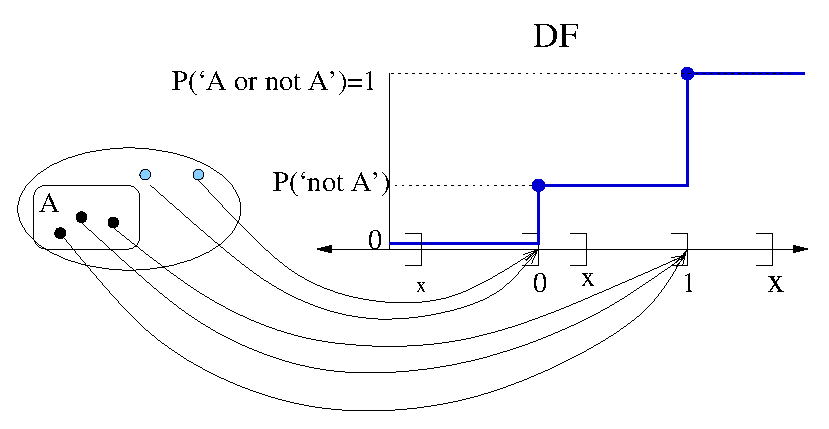
\includegraphics{figures/RVIndic}}
\end{figure}

\begin{Exercise}[title={Drawing discontinuous functions},label={drawDiscontFuncs}]
Identify the mistakes in how the  $\BB{1}_A$ is drawn as a discontinous function in Figure~\ref{F:RVIndic}.
%\ExePart
%\Question
%\subQuestion Show that...
%\subQuestion In this question...
%\subsubQuestion Show that...
%\subsubQuestion Conclude...
%\subQuestion Conclude.
%\Question Show that if $b > 1$...
%\ExePart
%\Question What happens to if $b=1$?
\end{Exercise}
\begin{Answer}
The first mistake is the solid vertical lines (blue) from $0$ in the domain or $x$-axis to $\p( \text{`not A'})$ in the range or $y$-axis and from $1$ in the domain to $1$ in the range. 
This is ill-defined for any function if we are to interpret that the elements in the domain, namely $0$ and $1$, are to be associated with the uncountably many image values in the range of the function, namely $[0,\p( \text{`not A'})]$ and $[\p( \text{`not A'}),1]$, respectively. 
So we should first replace them by dotted lines which merely help us track where the function jumped to at $0$ and $1$.

The second mistake is failing to emphasise that the value taken by the function at $0$ and $1$ is not $0$ and $\p( \text{`not A'})$, respectively. So it is best to introduce an empty circle like $\circ$ at $(0,0)$ and $(1,\p( \text{`not A'}))$ to indicate the points of discontinuity. The same mistakes should be fixed in the next Figure~\ref{F:RVABC}.
\end{Answer}

\begin{classwork}[A random variable with three values and eight sample points]\label{CW:ARVwith3Values}
Consider the RV $X$ of \hyperref[F:RVABC]{Figure \ref*{F:RVABC}}.  First draw this properly as done in Ex.~\ref{drawDiscontFuncs}. Let the events $A = \{\omega_1, \omega_2\}$, $B = \{\omega_3, \omega_4, \omega_5\}$ and $C = \{\omega_6, \omega_7,\omega_8 \}$.  Define the RV $X$ formally.  What sets should $\C{F}$ minimally include?  What do you need to do to make sure that $\C{F}$ is a sigma algebra?
\end{classwork}
\begin{figure}[htpb]
\caption{A RV $X$ from a sample space $\Omega$ with $8$ elements to $\Rz$ and its DF $F$.\label{F:RVABC}}
\centering   \makebox{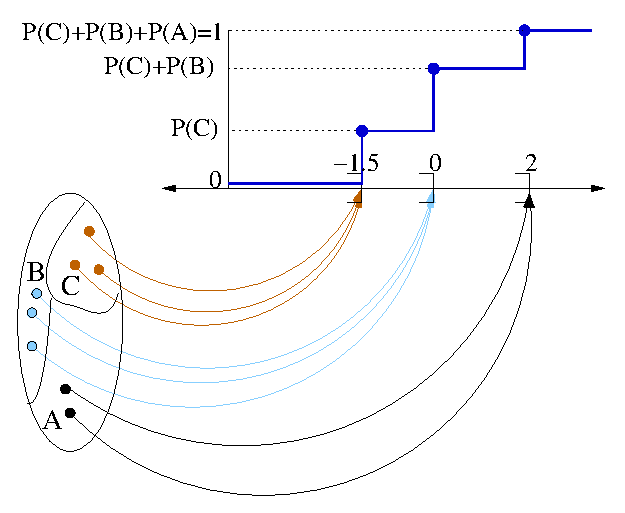
\includegraphics{figures/RV}}
\end{figure}

\begin{Exercise}[title={Fair coin toss RV},label={xFairCoinRV}]
Consider the {\em fair coin toss experiment}  with $\Omega= \{ \mathsf{H},\mathsf{T} \}$ and $P(\mathsf{H}) = P(\mathsf{T})=1/2$. \\[6pt] We can associate a $\bernoulli$ random variable $X$ (in Model~\ref{M:IndicatorIsaRV}) for the event that the coin lands as $\mathsf{H}$, with this experiment as follows:
\[X(\omega)=
\begin{cases}
1, & \text{if } \ \omega = \mathsf{H}\\
0, & \text{if } \ \omega = \mathsf{T}
\end{cases}
\]
Find the distribution function for $X$.
%\ExePart
%\Question
%\subQuestion Show that...
%\subQuestion In this question...
%\subsubQuestion Show that...
%\subsubQuestion Conclude...
%\subQuestion Conclude.
%\Question Show that if $b > 1$...
%\ExePart
%\Question What happens to if $b=1$?
\end{Exercise}
\begin{Answer}
The probability that $X$ takes on a specific value $x$ is:
$$
P(X = x) = P(\{\omega: X(\omega) = x \}) =
\begin{cases}
P(\emptyset) = 0, & \text{ if } \  x \notin \{0,1\} \\
P(\{\mathsf{T} \}) =  \frac{1}{2}, & \text{ if } \  x = 0\\
P(\{ \mathsf{H}\}) = \frac{1}{2}, & \text{ if } \  x = 1
\end{cases}
$$
or more simply,
\[
P(X=x)=
\begin{cases}
\frac{1}{2} & \text{if } x=0\\
\frac{1}{2} & \text{if } x=1\\
0 & \text{otherwise}
\end{cases}
\]
The distribution function for $X$ is:
$$
F(x) \;=\; P(X \leq x) \;=\; P(\{\omega: X(\omega) \leq x \})\; =\;
\begin{cases}
P(\emptyset) = 0, & \text{ if } \ -\infty < x < 0\\
P(\{\mathsf{T} \}) =  \frac{1}{2}, & \text{ if } \ 0 \leq x < 1\\
P(\{ \mathsf{H} , \mathsf{T} \}) = P(\Omega)  = 1,
& \text{ if } \ 1 \leq x < \infty
\end{cases}
$$
or more simply, $$
F(x)\; = \;P(X \leq x) \;=\;
\begin{cases}
 0, & \text{ if } \ -\infty < x < 0\\
 \frac{1}{2}, & \text{ if } \ 0 \leq x < 1\\
 1,
& \text{ if } \ 1 \leq x < \infty
\end{cases}
$$
\end{Answer}

\section{Discrete Random Variables}

When a RV takes at most countably many values from a discrete set $\Xz$, we call it a {\bf discrete} RV.  
Recall that a set $\Xz$ is said to be discrete if we can enumerate its elements, i.e., find an enumerating or counting function $\Xz \ni x \mapsto i \in\Nz$ that associates each element $x \in \Xz$ to a natural number $i \in \Nz$. 
So, $\Xz$ is either finite with $k$ elements in $\Xz = \{x_1,x_2,\ldots,x_k\}$ or countably infinite with the same cardinality as $\Nz$ with $\Xz = \{x_1,x_2,\ldots\}$. 
When $\Xz \subset \Rz$, we have a real-valued or $\Rz$-valued discrete random variable.

\begin{definition}[probability mass function (PMF)]
Let $X$ be a $\Rz$-valued discrete RV over a probability triple $(\Omega, \C{F},\p)$.  
We define the {\bf probability mass function} (PMF) $f$ of $X$ to be the function 
$f : \Rz \rightarrow [0,1]$ defined as follows:
\begin{framed}
\begin{equation}\label{Eq:DiscretePMF}
f(x) := \p(X=x) = \p( \ \{\omega: X(\omega) = x\} \ ) = 
\begin{cases}
\theta_i \quad \text{if $x=x_i \in \Xz$.}\\
0 \quad \text{otherwise}. 
\end{cases}
\end{equation}
\end{framed}
\end{definition}

The DF $F$ and PMF $f$ for a discrete RV $X$ satisfy the following:
\begin{enumerate}
\item  For any $x \in \Rz$, 
\begin{equation}\label{Eq:DiscreteDF}
\boxed{\p(X \leq x) = F(x)  = \sum_{x_i \leq x} f(x_i) = \sum_{x_i \leq x} \theta_i \ .}
\end{equation}
\item For any $a,b \in \Rz$ with $a<b$,
\begin{equation}\label{E:DRVFab}
\boxed{\p(a < X \leq b) = F(b) - F(a) = \sum_{a < x_i \leq b} \theta_i \ .}
\end{equation}
This is just the sum of all probabilities $\theta_i$ for which $x_i$ satisfies $a<x_i \leq b$. 
\item
From the fact that $\p(\Omega)=1$, we get that the sum of all the probabilties is $1$:
\begin{equation}\label{E:DRVsumofP}
\boxed{\sum_i \theta_i = 1 \ .}
\end{equation}
\item
When $X$ only has finitely many possibilities, say $k$ with $\Xz = \{x_1,x_2,\ldots,x_k\}$, then we may think of the probability $\p$ specified by $(\theta_1,\theta_2,\ldots,\theta_k)$ as a point in the \textbf{unit $(k-1)$ simplex}:
\begin{equation}\label{E:unitk-1simplex}
\Delta^{k-1} := \{ (\theta_1,\theta_2,\ldots,\theta_k) \in \Rz^{k} : \sum_i \theta_i = 1 \text{ and } \theta_i \geq 0, \text{ for all } i\}
\end{equation}
In particular when $X$ has only two possible values with $\Xz = \{x_1,x_2\}$ then $\theta_2=1-\theta_1$, so we can avoid subscripts and take $\theta := \theta_1$ and realize that the probability $\p$ is now specified by the point $(\theta,1-\theta)$ in the \textbf{unit $1$ simplex}:
\begin{equation}\label{E:unit1simplex}
\Delta^{1} := \{ (\theta,1-\theta) \in \Rz^2 : 0 \leq \theta \leq 1 \} \enspace .
\end{equation}
See \url{https://en.wikipedia.org/wiki/Simplex} for the images scribed on the board.
\end{enumerate}

\begin{framed}
DISCRETE RANDOM VARIABLES - SIMPLIFIED NOTATION\\

Notice that in equations \eqref{Eq:DiscretePMF}, \eqref{Eq:DiscreteDF} and \eqref{E:DRVFab} the use of the ``$\omega \in \Omega$'' notation, where random variables are defined as functions, is
much reduced. The reason is that in straightforward examples it is
convenient to associate the possible values $x_1,x_2,\dots$ with the
outcomes $\omega_1,\omega_2,\dots$ Hence, we can describe a discrete
random variable by the table:


$$\begin{array}{|c||c|c|c|c|}\hline
\textrm{Possible values: $x_i$} & x_1 & x_2 & x_3 & \ldots \\ \hline
&&&&\\
\textrm{Probability: $\p(X=x_i)=\theta_i$}& \theta_1 & \theta_2 & \theta_3 & \ldots \\ \hline
\end{array}
$$
It is customary to use $p_i$ instead of $\theta_i$ for the probabilities. But we try to avoid it as it will hurt us when we start doing Inference Theory soon!
\quad \\
Note that this table hides the more complex notation but it is still
there, under the surface. 
In Probability Theory I, you should be able to  work with and manipulate discrete random variables using the simplified notation given above. 
The same comment applies to the continuous random variables discussed later. But you are students of mathematics and should know more about what is ``under the hood''.

\end{framed}


Out of the class of discrete random variables we will define specific kinds as they arise often in applications.  We classify discrete random variables into three types for convenience as follows:
\begin{itemize}
\item {Discrete uniform random variables with finitely many possibilities}
\item {Discrete non-uniform random variables with finitely many possibilities}
\item {Discrete non-uniform random variables with (countably) infinitely many possibilities}
\end{itemize}

\begin{framed}
\begin{model}[Discrete Uniform]{\label{Df:DiscreteUniformRV}
We say that a discrete random variable $X$ is uniformly distributed over $k$ possible values in $\Xz=\{x_1,x_2,\ldots,x_k\}$ if its probability mass function is:
\begin{equation}\label{E:DiscreteUniformPMF}
f(x) =
\begin{cases}
\theta_i = \frac{1}{k} &  \quad\textrm{if } x=x_i, \quad\textrm{where } i=1,2, \ldots ,k \enspace, \\
0 & \quad\textrm{otherwise}\enspace.
\end{cases}
\end{equation}
The distribution function for the discrete uniform random variable $X$ is:
\begin{equation}\label{E:DiscreteUniformDF}
F(x) = \sum_{x_i\leq x} f(x_i) = \sum_{x_i\leq x} \theta_i =
\begin{cases}
0 &\quad \textrm{if }-\infty < x < x_1\enspace ,\\
\frac{1}{k}  & \quad \textrm{if }x_1 \leq x < x_2\enspace , \\
\frac{2}{k}  & \quad \textrm{if }x_2 \leq x < x_3\enspace , \\
\vdots & \\
\frac{k-1}{k}  & \quad \textrm{if }x_{k-1} \leq x < x_k\enspace , \\
1 & \quad \textrm{if }x_k \leq x < \infty\enspace .
\end{cases}
\end{equation}
}
The discrete uniform RV with values in $\Xz = \{1,2,\ldots,k\}$ is called the equi-probable $\demoivre(k)$ RV as we will see in the sequel. 
\end{model}
\end{framed}

\begin{example}\label{ExFairCoinRV}
The {\em fair coin toss experiment} of Exercise~\ref{xFairCoinRV} is an example of a discrete uniform random variable with finitely many possibilities. 
Its probability mass function is given by 
\[f(x)\;=\;\p(X=x)\;=\;
\begin{cases}
\frac{1}{2} & \text{if } x=0\\
\frac{1}{2} & \text{if } x=1\\
0 & \text{otherwise}
\end{cases}\] 
and its distribution function is given by
\[F(x)\; = \;\p(X \leq x) \;=\;
\begin{cases}
 0, & \text{ if } \ -\infty < x < 0\\
 \frac{1}{2}, & \text{ if } \ 0 \leq x < 1\\
 1,
& \text{ if } \ 1 \leq x < \infty
\end{cases}
\]
Let us sketch the probability mass function and distribution function for $X$ below. 
\begin{figure}[htbp]
\begin{center}
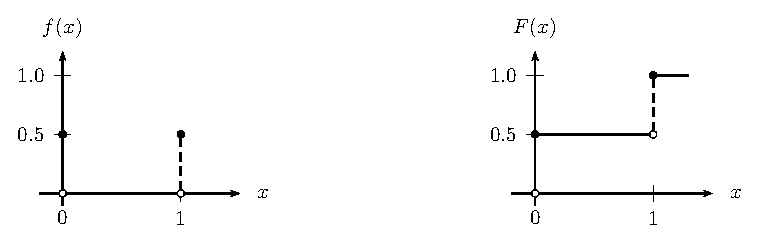
\includegraphics{pstricks/faircoinfF}
\caption{$f(x)$ and $F(x)$ of {\em the fair coin toss} random variable $X$, a discrete uniform RV on $\{0,1\}$.}
\end{center}
\end{figure}
\end{example}

\begin{example}[Fair dice RV]\label{Eg:FairDicerandomVariable}
Now consider the {\em toss a fair die} experiment and define $X$ to be the number that shows up on the top face. 
Note that here $\Omega$ is the set of numerical symbols $\{\mathsf{1}, \mathsf{2}, \mathsf{3}, \mathsf{4}, \mathsf{5}, \mathsf{6}\}$ 
that label each face while each of these symbols are associated with the real number 
$x \in \{1,2,3,4,5,6\}$. 
We can describe this random variable by the table 
$$\begin{array}{|c|cccccc|}\hline
\textrm{Possible values, $x_i$}&1&2&3&4&5&6 \\ \hline
&&&&&&\\
\textrm{Probability, $\theta_i$} &\frac{1}{6}&\frac{1}{6}&\frac{1}{6}&\frac{1}{6}&\frac{1}{6}&\frac{1}{6}\\ \hline
\end{array}
$$
Find the probability mass function and distribution function for this random variable, and sketch their graphs.

Solution:\\[4pt]
The probability mass function of this random variable is:
\[f(x)\;=\;\p(X=x)\;=\;
\begin{cases}
\frac{1}{6} & \text{if } x=1\\
\frac{1}{6} & \text{if } x=2\\
\frac{1}{6} & \text{if } x=3\\
\frac{1}{6} & \text{if } x=4\\
\frac{1}{6} & \text{if } x=5\\
\frac{1}{6} & \text{if } x=6\\
0 & \text{otherwise}
\end{cases}\] and the  distribution function is:
\[F(x)\; = \;\p(X \leq x) \;=\;
\begin{cases}
 0, & \text{ if } \ -\infty < x < 1\\
 \frac{1}{6}, & \text{ if } \ 1 \leq x < 2\\
\frac{1}{3}, & \text{ if } \ 2 \leq x < 3\\
\frac{1}{2}, & \text{ if } \ 3 \leq x < 4\\
\frac{2}{3}, & \text{ if } \ 4 \leq x < 5\\
\frac{5}{6}, & \text{ if } \ 5 \leq x < 6\\
 1,& \text{ if } \ 6 \leq x < \infty
\end{cases}
\]
\begin{figure}[htbp]
\begin{center}
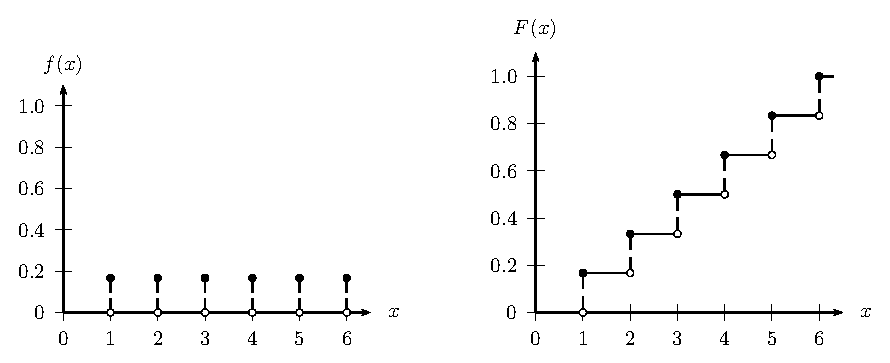
\includegraphics{pstricks/fairdiefF}
\caption{$f(x)$ and $F(x)$ of {\em the fair die toss} random variable $X$, a discrete uniform RV on $\{1,2,3,4,5,6\}$.}
\end{center}
\end{figure}
\end{example}

\begin{example}[Astragali with a Kiwi sheep ankle bone]\label{Eg:Astragali}
{\bf Astragali.} Board games involving chance
  were known in Egypt, 3000 years before Christ. The element of chance
  needed for these games was at first provided by tossing astragali, the
  ankle bones of sheep. These bones could come to rest on only four
  sides, the other two sides being rounded. The upper side of the bone,
  broad and slightly convex counted four; the opposite side broad and
  slightly concave counted three; the lateral side flat and narrow, one,
  and the opposite narrow lateral side, which is slightly hollow, six.
  You may examine an astragali of a kiwi sheep. \\[6pt] This is an example of a discrete
  non-uniform random variable with finitely many possibilities.  A surmised probability mass function with $f(4)=\frac{4}{10}$,
  $f(3)=\frac{3}{10}$, $f(1)=\frac{2}{10}$, $f(6)=\frac{1}{10}$ and
  distribution function are shown below.

\begin{figure}[htbp]
\begin{center}
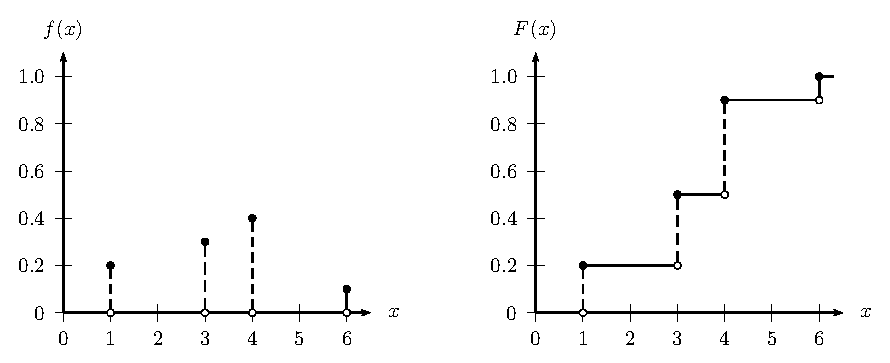
\includegraphics{pstricks/astragalifF}
\caption{$f(x)$ and $F(x)$ of surmised {\em astragali toss} random variable $X$, a discrete (non-uniform) RV on $\{1,2,3,4\}$.}
\end{center}
\end{figure}
\end{example}

\subsection{An Elementary Family of Bernoulli Random Variables}\label{S:ElemDiscRV}
In many experiments there are only two outcomes. For instance:

\bit
\item Flip a coin to see whether it is defective.
\item  Roll a die and determine whether it is a 6 or not.
\item  Determine whether it will be below $0$ degrees Celsius at 0600 hours in Uppsala tomorrow or not.
\eit

Performing such an experiment $\E{E}$ once to see if an event of interest $A$ occurs is called a {\bf Bernoulli trial} and its probability model over a triple $(\Omega,\C{F},\p)$, with $A \in \C{F}$, given by  the Indicator Function $\BB{1}_A$ in Model~\ref{M:IndicatorIsaRV} is called the $\bernoulli$ RV. 

If we do not know the probability $\theta$ that `$A$ occurs', i.e., the $\bernoulli$ RV will equal $1$, then we can define a whole family of $\bernoulli$ RVs for each 
$\theta \in [0,1]$ or more precisely for each $(\theta, 1-\theta) \in \Delta^1$, the unit $1$-Simplex.
Note that this family includes the fair Bernoulli trial of Example~\ref{ExFairCoinRV} when $\theta=0.5$. Let us formalise this as the $\bernoulli(\theta)$ RV for each $\theta \in [0,1]$ next.

\begin{model}[$\bernoulli(\theta)$ RV]
Given a parameter $\theta \in [0,1]$, the probability mass function (PMF) for the $\bernoulli(\theta)$ RV $X$ is:
\begin{equation}\label{E:Bernoullipdf}
f(x;\theta)= \theta^x (1-\theta)^{1-x} \BB{1}_{\{0,1\}}(x) =
\begin{cases}
\theta & \text{if $x=1$,}\\
1-\theta & \text{if $x=0$,}\\
0 & \text{otherwise}
\end{cases}
\end{equation}
and its DF is:
\begin{equation}
F(x;\theta) =
\begin{cases}
1 & \text{if $1 \leq x$,}\\
1-\theta & \text{if $0 \leq x < 1$,}\\
0 & \text{otherwise}
\end{cases}
\end{equation}
We emphasise the dependence of the probabilities on the parameter $\theta$ by specifying it following the semicolon in the argument for $f$ and $F$ and by subscripting the probabilities, i.e.~$\p_{\theta}(X=1)=\theta$ and $\p_{\theta}(X=0)=1-\theta$.
\end{model}
\begin{figure}[htpb]
\centering   \makebox{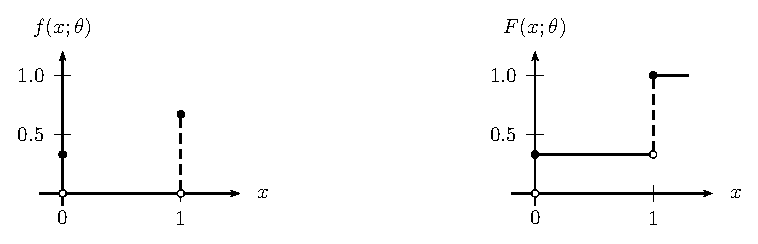
\includegraphics{pstricks/bernouliThetafF}}
\caption{PMF $f(x;\theta)$ and DF $f(x;\theta)$ with $\theta = 0.33$. You should see how PMF and DF change as $\theta$ goes from $0$ to $1$}
\end{figure}

\subsection{Independent $\bernoulli$ Trials}

Random variables make sense for a series of trials as well as just a single trial of an experiment.  
We now look at  what happens when we perform a sequence of independent Bernoulli trials.  
For instance:
\bit
\item Flip a coin 10 times; count the  number of heads 
\bit
\item by possibly allowing for the coin's $\p(\mathsf{H})$ to change each time because each of them are manufactured in a terrible mint.
\eit
\item Test 50 randomly selected circuits from an assembly line; count
  the  number of defective circuits.
\item  Roll a die 100 times; count the  number of sixes you throw.
\item Provide a property near a particular bridge in our archipelago with flood insurance
  for 20 years; count the number of years, during the 20-year period,
  during which the property is flooded. Note: we assume that flooding is
  independent from year to year, and that the probability of flooding is the same
  each year.
\eit

Since the $\bernoulli(\theta)$ RV has only two outcomes, i.e., simple events, we know how to obtain the probability of each of the two outcomes in a given $\bernoulli$ trial with the probability given by the deterministic variable or parameter $\theta$. 
Now consider doing more than one trial so we have sequence of $\bernoulli(\theta_i)$ trials, say,
\[
X_i \sim \bernoulli(\theta_i) \text{ with } i \in \mathbb{N} \enspace ,
\] 
with each $\theta_i \in [0,1]$ being possibly unkown but fixed as a parameter. 
Now, if we assume independence across trials, so one trial's outcome does not affect the outcome of any of the other trials, in the sense of Definition~\ref{D:IndOfSeqOfEvents} 
about \emph{independence of a sequence of events}, then we can obtain the probability of the entire sequence of outcomes for this sequence of \textbf{independently distributed} $\bernoulli(\theta_i)$ \textbf{trails} which can be any infinite sequence of $0$'s and $1$'s, i.e., any element of $\{0,1\}^{\infty}$, by simply multiplying the corresponding probabilities given by $\theta_i$'s in $(\theta_1,\theta_2,\ldots) \in [0,1]^{\infty}$, an infinite dimensional parameter space, as follows:
\begin{eqnarray}\label{Eq:probofindependentBernoullithetaiTrials}
\p(x; (\theta_1,\theta_2,\ldots)) &=& \prod_i f(x_i;\theta_i)= \prod_i \theta_i^{x_i} (1-\theta_i)^{1-x_i} \BB{1}_{\{0,1\}}(x_i), \\
&~& \qquad \qquad \text{ where } x:= (x_1,x_2,\ldots) \in \mathbb{X}_{\infty} = \{0,1\}^{\infty} := \{0,1\} \times \{0,1\} \times \cdots \notag
\end{eqnarray}
By further assuming that all the $\theta_i$'s are identical, say $\theta = \theta_1 = \theta_2 = \cdots$, with $\theta \in [0,1]$, a one-dimensional parameter space, we get the much simpler expression for the \textbf{independent and identically distributed (IID)} $\bernoulli(\theta)$ \textbf{trails} as follows:
\begin{eqnarray}\label{Eq:probofindependentIdenticalBernoullithetaTrials}
\p(x; \theta) &=& \prod_i f(x_i;\theta)= \prod_i \theta^{x_i} (1-\theta)^{1-x_i} \BB{1}_{\{0,1\}}(x_i) =  \BB{1}_{\{0,1\}^{\infty}}(x) \, \theta^{\sum_i x_i} (1-\theta)^{\sum_i(1-x_i)} \notag\\
&=&  
\begin{cases}
\theta^{\sum_i x_i} (1-\theta)^{n-\sum_i x_i} & \text{if $x:= (x_1,x_2,\ldots) \in \mathbb{X}_{\infty} = \{0,1\}^{\infty}$}\\ 
0 & \text{otherwise}\enspace .
\end{cases}
\end{eqnarray}

Remembering that all other RVs can be derived from such IID $\bernoulli(\theta)$ trials using $\theta=1/2$, as we will see in the sequel, 
we are ready to take a tour through some common discrete and continuous random variables that are useful in many applications.
 
\subsection{Some Common Discrete Random Variables}\label{S:SomeCommonDiscreteRVs}

Let us start with the simplest example to fix ideas carefully.
\begin{example}[Waiting For the First Heads]\label{Ex:WaitinfFor1stHeads}
Suppose our experiment is to toss a fair coin independently and
  identically (that is, the same coin is tossed in essentially the same
  manner independent of the other tosses in each trial) as often as
  necessary until we have a head, $\mathsf{H}$.  Let the random
  variable
  $X$ denote the \emph{Number of trials until the first $\mathsf{H}$ appears}.\\[4pt]
Let's first find the probability mass function of $X$.

Now $X$ can take on the values
$\{1,\,2,\,3,\,\ldots\}$, so we  have a  non-uniform random
variable with infinitely many possibilities.  Since
\ba{
&f(1)\; =\; \p(X=1)\;=\;P(\mathsf{H})\;=\;\frac{1}{2}\enspace , & \\
&f(2)\; =\; \p(X=2)\;=\;P(\mathsf{TH})\;=\;\frac{1}{2}\cdot \frac{1}{2}\;= \;\left(\frac{1}{2}\right)^2 \enspace , \\
&f(3)\; = \; \p(X=3)\;=\;P(\mathsf{TTH})\;=\;\frac{1}{2}\cdot \frac{1}{2}\cdot \frac{1}{2}\;= \;\left(\frac{1}{2}\right)^3 \enspace, \qquad \textrm{etc.}
}the  probability mass function of $X$ is:
$$f(x)\; =\; \p(X=x)\;=\;\left(\frac{1}{2}\right)^x, \quad x=1,2,\dots \enspace.$$
\end{example}

\bigskip

In the previous Example, % \ref{Ex:WaitinfFor1stHeads},  %%cross-referencing needs fixing as the counters are clashing need change in new_base macro file
noting that we have independent trials, we get:

\[f(x)\; = \;\p(X=x)\;=\;\p(\mathsf{\underbrace{\mathsf{TT}\ldots\mathsf{T}}_{n-1}\mathsf{H}})\;=\; \p(\mathsf{T})^{x-1}\,\p(\mathsf{H})\;=\;
\left(\frac{1}{2}\right)^{x-1}\,\frac{1}{2}\,.\]
More generally, let there be two possibilities, success ($\mathsf{S}$) or failure
($\mathsf{F}$), with  $\p(\mathsf{S})=  \theta$  and \newline $\p(\mathsf{F})=1-\theta$ so that:
\[\p(X=x)\;=\;\p(\underbrace{\mathsf{F F} \ldots \mathsf{F}}_{x-1}\mathsf{S})\;=\; (1 - \theta)^{x-1}\, \theta\,.\]

 This is called a {\bf geometric random variable} with ``success
 probability'' parameter $\theta$. We can spot a geometric distribution
 because there will be  {\em a sequence of independent  trials with a constant
   probability  of success. We are counting the number of trials until
   the first success appears.} Let us define this random variable formally next.

\begin{model}[$\geometric(\theta)$ RV]\label{M:GeomRV}
Given a parameter $\theta \in (0,1)$, the PMF of the $\geometric(\theta)$ RV $X$ is
\begin{equation}\label{E:Geometricpdf}
f(x;\theta) =
\begin{cases}
\theta(1-\theta)^{x} & \text{if $x \in \Zz_+ := \{0,1,2,\ldots \}$} \\
0 & \text{otherwise}
\end{cases}
\end{equation}
It is straightforward to verify that $f(x;\theta)$ is indeed a PMF :
\[
\sum_{x=0}^{\infty} f(x;\theta) = \sum_{x=0}^{\infty} \theta(1-\theta)^{x}
= \theta \left( \frac{1}{1-(1-\theta)} \right) =  \theta \left( \frac{1}{\theta} \right) = 1
\]

{\scriptsize
The above equality is a consequence of the geometric series identity \eqref{E:GeomSeries} with $a=\theta$ and $\vartheta:=1-\theta$:
\begin{equation}\label{E:GeomSeries}
 \sum_{ x =0}^{\infty} a \vartheta^x = a \left( \frac{1}{1-\vartheta} \right) , \ \text{provided, } 0 < \vartheta < 1 \ .
\end{equation}
\begin{proof}
\[
a+a\vartheta+a\vartheta^2+\cdots+a\vartheta^n
= \sum_{0 \leq x \leq n} a \vartheta^x
= a+ \sum_{1 \leq x \leq n} a \vartheta^x
= a +  \vartheta  \sum_{1 \leq x \leq n} a \vartheta^{x-1}
= a +  \vartheta  \sum_{0 \leq x \leq n-1} a \vartheta^{x}
= a +  \vartheta  \sum_{0 \leq x \leq n} a \vartheta^{x} - a \vartheta^{n+1}
\]
Therefore,
\begin{eqnarray}
\sum_{0 \leq x \leq n} a \vartheta^x
&=&  a +  \vartheta  \sum_{0 \leq x \leq n} a \vartheta^{x} - a \vartheta^{n+1} \notag \\
\left( \sum_{0 \leq x \leq n} a \vartheta^x \right) - \left( \vartheta  \sum_{0 \leq x \leq n} a \vartheta^{x} \right)
&=&  a  - a \vartheta^{n+1} \notag \\
\left( \sum_{0 \leq x \leq n} a \vartheta^x \right) (1-\vartheta)
&=&  a (1 -  \vartheta^{n+1}) \notag \\
\sum_{0 \leq x \leq n} a \vartheta^x
&=&  a \left( \frac{1 -  \vartheta^{n+1}}{1-\vartheta} \right) \notag\\
 \sum_{ x =0}^{\infty} a \vartheta^x  := \lim_{n \rightarrow \infty} \sum_{0 \leq x \leq n} a \vartheta^x
&=&  a \left( \frac{1}{1-\vartheta} \right) , \ \text{provided, } 0 < \vartheta < 1 \notag
\end{eqnarray}
\end{proof}
}
The outcome of a $\geometric(\theta)$ RV can be thought of as ``the number of tosses needed before the appearance of the first `Head' when tossing a coin with probability of `Heads' equal to $\theta$ in a independent and identical manner.''
\end{model}

\begin{figure}[htpb]
\caption{PMF of $X \sim \geometric(\theta=0.5)$ and the relative frequency histogram based on $100$ and $1000$ samples from $X$ according to Simulation~\ref{SIM:Geometric} and Labwork~\ref{LW:RelFreqHistForGeomSims} you will see in the sequel.\label{F:PlotPdfSimHistGeomthetaHalf}}
\centering   \makebox{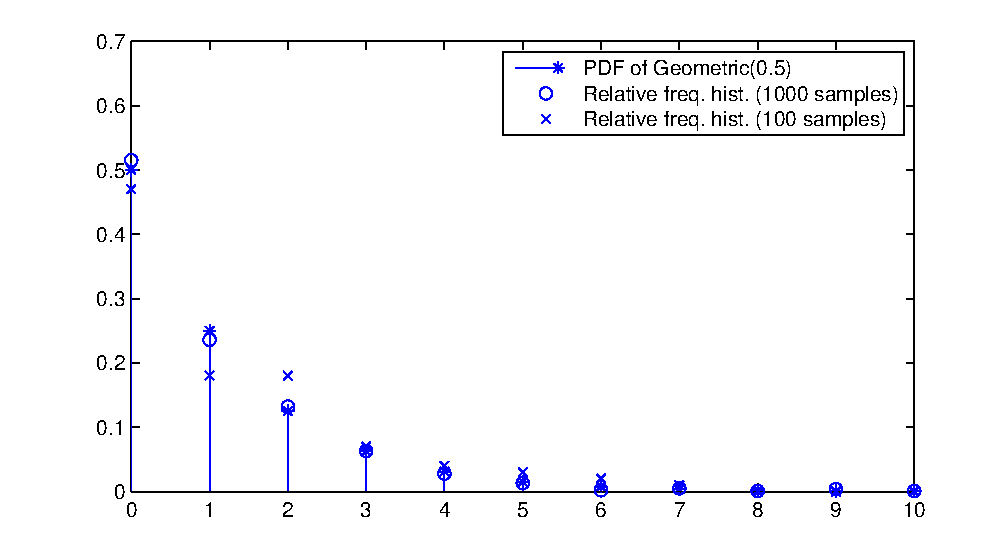
\includegraphics[width=6.50in]{figures/PlotPdfSimHistGeomthetaHalf}}
\end{figure}

\begin{Exercise}[title={Coupon Collector's Probem},label={xCouponCollPr}]
Recall the Coupon Collector's Problem from lectures.%TODO
\end{Exercise}
\begin{Answer}
This was done in week 1. Get notes from your mates or wait until Raaz scribes for virtual convenience.
\end{Answer}

\begin{example}\label{Exmp:Flip10times}
Suppose we flip a coin 10 times and count the number of heads.  Let's consider the probability of getting three  heads, say. 
The probability that the first three flips are heads and the last  seven  flips are tails, \emph{in order},  is \[ \underbrace{\frac{1}{2} \frac{1}{2}
    \frac{1}{2}}_{3 \text{ successes}}
  \,\underbrace{\frac{1}{2} \frac{1}{2} \dots \frac{1}{2}}_{7
    \text{ failures}} \, .\]
But there are \[\binom{10}{3} \;=\; \frac{10!}{7!\, 3!}\;=\;120 \] ways
of ordering three heads and seven tails,  so the
  probability  of getting three  heads and seven  tails \emph{in any order},  is\[\p( \text{`} 3 \text{ heads'}) \;=\; \binom{10}{3}  \left(\frac{1}{2}\right)^3
  \;\left(\frac{1}{2}\right)^7 \;\approx\; 0.117\]
\end{example}

We can describe  this sort of situation by considering a random variable $X$ which counts the number of successes, as follows:

\remove{
The RV $Y$ in \hyperref[T:T3XRVs]{Table \ref*{T:T3XRVs}} may be generalized to an experiment $\E{E}_{\theta}^{n}$ with $n$ coin tosses.  
%}% end remove
Let $X_i$ be the Indicator function of the event `Heads on the $i$-th toss' as before.  Then $Y$ defined by,
 \[
 Y := \sum_{i=1}^n X_i := X_1 + X_2 + \cdots + X_n  \ ,
 \]
is the number of `Heads' in $n$ tosses.  
%\remove{
Akin to the second row of \hyperref[T:T3XRVs]{Table \ref*{T:T3XRVs}}, for the `Toss $n$ times' experiment $\E{E}_{\theta}^{n}$ the
%} 
RV $Y$ as defined above will take values in $\{0,1,2,\ldots,n\}$ and is therefore a discrete RV.  This is called the Binomial RV as defined next.  
%\remove{
But, first we remind ourselves of some elementary definitions involving arrangements of objects from a collection (recall \hyperref[S:PermsFactsCombs]{Section~\ref*{S:PermsFactsCombs}}).
%}%end remove
}

\begin{model}[$\binomial(n,\theta)$ RV]\label{M:binomial}
Let the RV $X=\sum_{i=1}^n X_i$ be the sum of $n$ independent and identically distributed $\bernoulli(\theta)$ RVs, i.e.:
\[
X=\sum_{i=1}^n X_i, \qquad X_1,X_2,\ldots,X_n \overset{\IID}{\sim} \bernoulli(\theta) \ .
\]
Given two parameters $n$ and $\theta$, the PMF of the $\binomial(n,\theta)$ RV $X$ is:
\begin{equation}
 f(x; n,\theta) =
 \begin{cases}
 \displaystyle\binom{n}{x} \theta^x (1-\theta)^{n-x} & \text{if $x \in \{0,1,2,3,\ldots,n\}$} \ ,\\
 0 & \text{otherwise}
 \end{cases}
 \end{equation}
where, $\binom{n}{x}$ is:
\[
\binom{n}{x} = \frac{n(n-1)(n-2)\ldots(n-x+1)}{x(x-1)(x-2)\cdots (2)(1)} =  \frac{n !}{x! (n-x)!} \ .
 \]
$\binom{n}{x}$ is read as ``$n$ choose $x$.''
 \end{model}
{\bf A Quick Justification:}  The argument from Example~\ref{Exmp:Flip10times} generalises as follows.  
Since the trials are independent and identical, the probability of $x$ successes followed by $n-x$ failures,
\emph{in order},  is
given by
\[\underbrace{\mathsf{SS} \dots \mathsf{S}}_{x}\underbrace{\mathsf{FF} \dots \mathsf{F}}_{n-x}\;=\;\theta^x (1-\theta)^{n-x} \,.\]


Since the $n$ symbols $\mathsf{S S} \dots \mathsf{S} \,\mathsf{F F} \dots \mathsf{F}$ may be arranged in
\[\displaystyle\binom{n}{x} \;=\; \frac{n!}{(n-x)! x!}\]
ways, the probability of  $x$ successes and  $n-x$ failures,
\emph{in any order},  is
given by
\[\displaystyle\binom{n}{x}\;\theta^x (1-\theta)^{n-x}\,.\]

{\scriptsize
\begin{proof} This is only a sketch. A formal proof should start with the mathematical induction for the very formula for the binomial coefficient.

Observe that for the $\binomial(n,\theta)$ RV $X$, $\p(X=x) = f(x;n,\theta)$ is the probability that $x$ of the $n$ $\bernoulli(\theta)$ trials result in an outcome of $1$'s.  Next note that if all $n$ $X_i$'s are $0$'s, then $X=0$, and if all $n$ $X_i$'s are $1$'s, then $X=n$.  In general, if some of the $n$ $X_i$'s are $1$'s and the others are $0$, then $X$ can only take values in $\{0,1,2,\ldots,n\}$ and therefore $f(x;n,\theta)=0$ if $x \notin \{0,1,2,\ldots,n\}$.

Now, let us compute $f(x;n,\theta)$ when $x\in\{0,1,2,\ldots,n\}$.  Consider the set of indices $\{1,2,3,\ldots,n\}$ for the $n$ IID $\bernoulli(\theta)$ RVs $\{X_1,X_2,\ldots,X_n\}$.  Now choose $x$ indices from $\{1,2,\ldots,n\}$ to mark those trials in a particular realization of $\{x_1,x_2,\ldots,x_n\}$ with the Bernoulli outcome of $1$.  The probability of each such event is $\theta^x (1-\theta)^{n-x}$ due to the IID assumption.  For each realization $\{x_1,x_2,\ldots,x_n\} \in \{0,1\}^{n} := \{ \text{all binary $(0-1)$ strings of length $n$}\}$, specified by a choice of $x$ trial indices with Bernoulli outcome $1$, the binomial RV $X=\sum_{i=1}^n X_i$ takes the value $x$.  Since there are exactly $\binom{n}{x}$ many ways in which we can choose $x$ trial indices (with outcome $1$) from the set of $n$ trial indices $\{1,2,\ldots,n\}$, we get the desired product for $f(x; n,\theta) = \binom{n}{x} \theta^x (1-\theta)^{n-x}$ when $x \in \{0,1,\ldots,n\}$.
\end{proof}
}
\begin{figure}[htpb]
\caption{PDF of $X \sim \binomial(n=10,\theta=0.5)$ and the relative frequency histogram based on $100,000$ samples from $X$ obtained according to Simulation~\ref{SIM:BinomialFromGeoms}.\label{F:PlotPdfSim10000HistBinomByGeomsn10thetaHalf}} % TODO check which of two simulation algs is coming from
\centering   \makebox{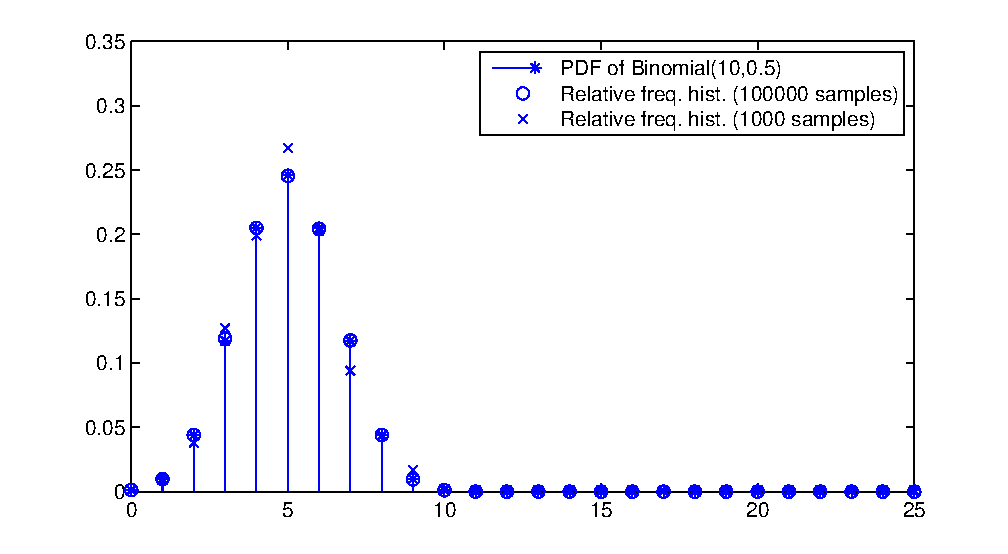
\includegraphics[width=6.50in]{figures/PlotPdfSim10000HistBinomByGeomsn10thetaHalf}}
\end{figure}

\begin{example}\label{Eg:70f10recover}
Find the probability that seven of ten persons will recover from a
  tropical disease where the probability is
  identically $0.80$ that any one of them will recover from the
  disease.

{Solution:}\\[4pt]
We can assume independence here, so we have a binomial
situation with  $x=7$, $n=10$, and $\theta=0.8$. Substituting these into the formula for the probability mass function for $\binomial(10,0.8)$ random variable, we get:
\ba{f(7;10,0.8)&\;=\;\binom{10}{7} \times (0.8)^7 \times
  (1-0.8)^{10-7}\\[6pt]
& \;= \frac{10!}{(10-7)! 7!} \times (0.8)^7 \times (1-0.8)^{10-7}\\[6pt]
&=\; 120 \times (0.8)^7 \times (1-0.8)^{10-7} \qquad ^*\text{{\scriptsize In the exam you can give your answer as such an expression.}}\\[6pt]
& \approx \; 0.20
}
\end{example}

\begin{example}\label{Eg:alteast2_6s}
{Compute the probability of obtaining {\em at least two
    $\mathsf{6}$'s} in rolling a fair die independently and identically
  four times.}

{Solution:}\\[4pt]
{In any given toss let $\theta=\p(\{\mathsf{6}\})=1/6$,
$1-\theta=5/6$, $n=4$.

The event {\em at least two $\mathsf{6}$'s} occurs if we obtain two or
three or four $\mathsf{6}$'s.  Hence the answer is:
\ba{
\p(\text{{\em at least two $\mathsf{6}$'s}})&\;=\; f\left(2;4,\frac{1}{6}\right)\;+\;f\left(3;4,\frac{1}{6}\right)\;+\;f\left(4;4,\frac{1}{6}\right) \\[6pt]
&=\; \binom{4}{2}\left(\frac{1}{6}\right)^2\left(\frac{5}{6}\right)^{4-2}\;+\;
\binom{4}{3}\left(\frac{1}{6}\right)^3\left(\frac{5}{6}\right)^{4-3}\;+\;
\binom{4}{4}\left(\frac{1}{6}\right)^{4}\left(\frac{5}{6}\right)^{4-4}\\[6pt]
&=\;\frac{1}{6^4}\,\left(6\cdot25+4\cdot5+1\right)\\[6pt]
&\approx \;0.132
}
}
\end{example}

To make concrete sense of the $\binomial(n,\theta)$ and other more sophisticated concepts in the sequel, let us take a historical detour into some origins of statistical thinking in 19th century England.

\subsubsection{Sir Francis Galton's Quincunx}\label{S:Quincunx}
This section is introduced to provide some forms for a kinesthetic (hands-on) and visual understanding of some elementary statistical distributions and laws.  The following words are from Sir Francis Galton, F.R.S., {\em Natural Inheritance}, pp.~62-65, Macmillan, 1889.  In here you will already find the kernels behind the construction of $\binomial(\theta)$ RV as sum of IID $\bernoulli(\theta)$ RVs, Weak Law of Large Numbers, Central Limit Theorem, and more.  We will mathematically present these concepts in the sequel as a way of giving precise meanings to Galton's observations with his Quincunx.
{\it ``{\em The Charms of Statistics}.--It is difficult to understand why statisticians commonly limit their inquiries to Averages, and do not revel in more comprehensive views.  Their souls seem as dull to the charm of variety as that of the native of one of our flat English counties, whose retrospect of Switzerland was that, it its mountains could be thrown into its lakes, two nuances would be got rid of at once.  An Average is but a solitary fact, whereas if a single other fact be added to it, an entire Normal Scheme, which nearly corresponds to the observed one, starts potentially into existence.

Some people hate the very name of statistics, but I find them full of beauty and interest.  Whenever they are not brutalised, but delicately handled by the higher methods, and are warily interpreted, their power of dealing with complicated phenomenon is extraordinary.  They are the only tools by which an opening can be cut through the formidable thicket of difficulties that bars the path of those who pursue the Science of man.}

\begin{figure}[htpb]
\caption{Figures from Sir Francis Galton, F.R.S., {\em Natural Inheritance}, , Macmillan, 1889.\label{F:GaltonFigure78923}}
\mbox{\subfigure[FIG.~7, FIG.~8, and FIG.~ 9 (p.~63)]{\hspace{-0.15cm} 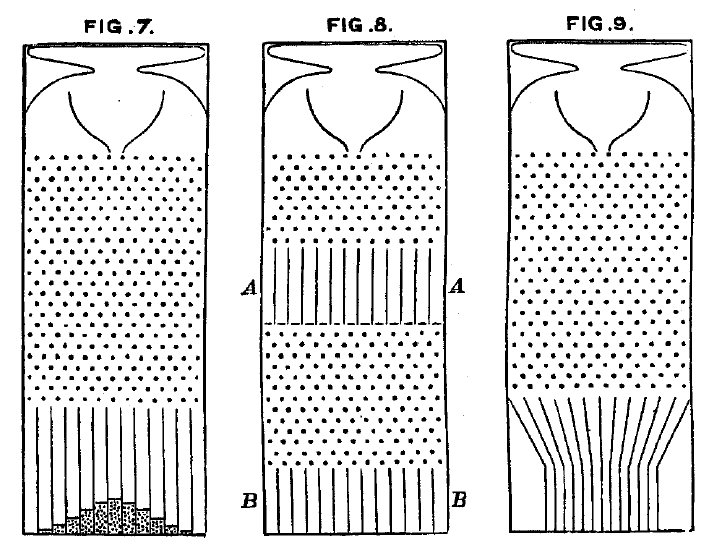
\includegraphics[width=3.250in,clip=,angle=0]{figures/GaltonsFigs789}} \hspace{-0.5cm} \subfigure[FIG.~2 and FIG.~3 (p.~38)]{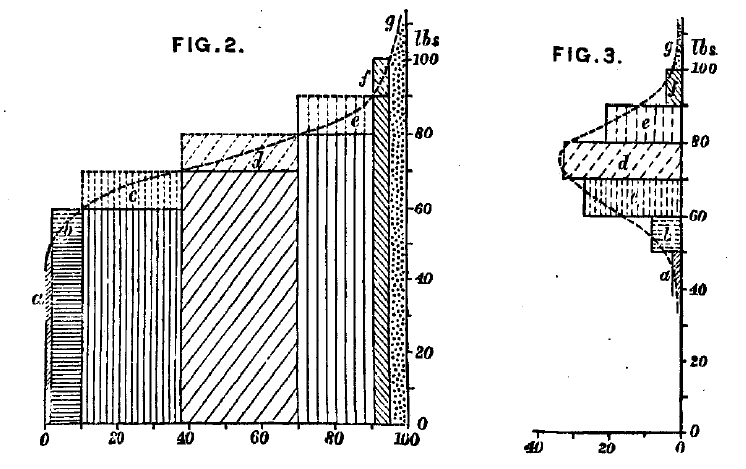
\includegraphics[width=3.40in,clip=,angle=0]{figures/GaltonsFigs23}} }
\end{figure}

{\it {\em Mechanical Illustration of the Cause of the Curve of Frequency}.--The Curve of Frequency, and that of Distribution, are convertible : therefore if the genesis of either of them can be made clear, that of the other also becomes intelligible.  I shall now illustrate the origin of the Curve of Frequency, by means of an apparatus shown in Fig.~7, that mimics in a very pretty way the conditions
on which Deviation depends.  It is a frame glazed in front, leaving a depth of about a quarter of an inch behind the glass.  Strips are placed in the upper part to act as a funnel.  Below the outlet of the funnel stand a succession of rows of pins stuck squarely into the backboard, and below these again are a series of vertical compartments.  A charge of small shot is inclosed.  When the frame is held topsy-turvy, all the shot runs to the upper end; then, when it is turned back into its working position, the desired action commences.  Lateral strips, shown in the diagram, have the effect of directing all the shot that had collected at the upper end of the frame to run into the wide moutn of the funnel.  The shot passes through the funnel and issuing from its narrow end, scampers deviously down through the pins in a curious and interesting way; each of them darting a step to the right or left, as the case may be, every time it strikes a pin.  The pins are disposed in a quincunx fashion, so that every descending shot strikes against a pin in each successive row.  The cascade issuing from the funnel broadens as it descends, and, at length, every shot finds itself caught in a compartment immediately after freeing itself from the last row of pins.  The outline of the columns of shot that accumulate in the successive compartments approximates to the Curve of Frequency (Fig.~3, p.~38), and is closely of the same shape however often the experiment is repeated.  The outline of the columns would become more nearly identical with the Normal Curve of Frequency, if the rows of pins were much more numerous, the shot smaller, and the compartments narrower; also if a larger quantity of shot was used.}

{\it The principle on which the action of the apparatus depends is, that a number of small and independent accidents befall each shot in its career.  In rare cases, a long run of luck continues to favour the course of a particular shot towards either outside place, but in the large majority of instances the number of accidents that cause Deviation to the right, balance in a greater or less degree those that cause Deviation to the left.  Therefore most of the shot finds its way into the compartments that are situated near to a perpendicular line drawn from the outlet of the funnel, and the Frequency with which shots stray to different distances to the right or left of that line diminishes in a much faster ratio than those distances increase.  This illustrates and explains the reason why mediocrity is so common.'' }


We now consider the last of our common discrete random variables for now, the {\bf Poisson} case.  
A Poisson random variable counts the number of times an event occurs.

We might, for example, ask:
\bit
\item How many customers visit Cafe Angstrom each day?
\item How many sixes  are scored  in a cricket season? {\scriptsize Cricket is a game played in the English-speaking worlds.}
\item How many bombs hit a city block in south London during World War II?
\eit

A Poisson experiment has the following characteristics:

\bit
\item The average  rate of an event occurring is known. This rate is constant.
\item  The probability that an event  will occur during a short continuum is proportional to the size of the continuum.
\item  Events occur independently.
\eit

The number of events occurring  in a Poisson experiment is referred to as a
{\bf Poisson random variable}.

\begin{model}[$\poisson(\lambda)$ RV]\label{M:Poisson}
Given a real parameter $\lambda>0$, the discrete RV $X$ is said to be $\poisson(\lambda)$ distributed if $X$ has PDF:
\begin{equation}\label{E:Poissonpdf}
f(x;\lambda) =
\begin{cases}
 \frac{ e^{-\lambda} \lambda^x}{x!} & \text{if $x \in \Zz_+ := \{0,1,2,\ldots\}$} \ , \\
0 & \text{otherwise} \ .
\end{cases}
\end{equation}

Note that the PDF integrates to $1$:
\[
\sum_{x=0}^{\infty} f(x;\lambda)
= \sum_{x=0}^{\infty}  \frac{ e^{-\lambda} \lambda^x}{x!}
=  e^{-\lambda} \sum_{x=0}^{\infty}  \frac{\lambda^x}{x!}
=  e^{-\lambda} e^{\lambda}
= 1 \ ,
\]
where we exploit the Taylor series of $e^{\lambda}$ to obtain the second-last equality above.

We interpret $X$ as the number of times an event occurs during a
specified continuum given that the average value in the continuum is
$\lambda$. 
\end{model}


\begin{example}{\label{eqn:poi_cars}}
If on the average, 2 cars enter a certain parking lot per minute,
  what is the probability that during any given minute three cars or
  fewer
  will enter the lot?

Think: Why are the assumptions for a Poisson random variable likely to
be correct here?

Note: Use calculators, or Excel or Maple, etc. In an exam you may be given needed values from Poisson tables.


Let the random variable $X$ denote the number of cars
  arriving per minute. Note that the continuum is 1 minute here. Then  $X$ can be considered to have  a Poisson distribution
  with $\lambda=2$ because 2 cars enter on
average.

\medskip

The probability that three cars or fewer enter the lot is:
\ba{\p(X\leq 3)&\;=\;
f(0;2)+f(1;2)+f(2;2)+f(3;2)\\
&\;=\;e^{-2}\left(\frac{2^0}{0!}+\frac{2^1}{1!}+\frac{2^2}{2!}+\frac{2^3}{3!}\right) \qquad ^*\text{\scriptsize{This is a perfectly fine answer in the exam.}}\\
&\;=\;0.857 \quad 
\quad (\text{3 sig. fig.})
}
\end{example}


\begin{example}[Arrivals at a Service Station]\label{Eg:serviceStation}
The proprietor of a service station finds that, on average, $8$
  cars arrive \emph{per hour} on Saturdays. What is the probability
  that during a randomly chosen $15$ \emph{minute period} on a Saturday:
\be
\item[(a)] No cars arrive?
\item[(b)]  At least three cars arrive?
\ee

Solution:\\[4pt]
Let the random variable $X$ denote the number of cars
  arriving in a 15 minute interval. The continuum is 15 minutes here so
  we need the average number of cars that arrive in a 15 minute
  period, or $\frac{1}{4}$ of an hour.  We know that 8 cars arrive per
  hour, so  $X$ has a Poisson distribution
  with
\[\lambda \;=\; \frac{8}{4}\;=\; 2\,.\]

\be
\item[(a)]

\[\p(X=0)\;=\;  f(0; 2)\;=\;  \frac{ e^{-2} 2^0}{0!}\;=\; 0.135 \quad (\text{3 sig. fig})\]

\item[(b)]
 \ba{\p(X\geq  3 )&\;=\;  1\,-\, \p(X <  3)\\
&\;=\;  1\,-\, \p(X = 0)\,-\, \p(X = 1)\,-\, \p(X = 2)\\
&\;=\;  1\,-\, f(0; 2) \,-\, f(1; 2) \,-\, f(2; 2) \\
&\;=\;1-  0.1353 \,-\, 0.2707\,-\, 0.2707\\
&\;=\; 0.323 \quad (\text{3 sig. fig.})}
\ee
\end{example}

\begin{rem}
In the binomial case where $\theta$ is small and $n$ is large, it can be shown that the
binomial distribution with parameters $n$ and $\theta$ is closely
approximated by the Poisson distribution having $\lambda = n \theta$. The
smaller the value of $\theta$ and larger the value of $n$, the better the approximation.

In the sequel we will see more formally, after understanding notions of convergence of RVs, that the sum of a sequence of $n$ IID $\bernoulli(\theta)$ RVs with $\lambda = n \theta$ converges to the $\poisson(\lambda)$ RV as $n \to \infty$ and $\theta \to 0$ in a specific sense.
\end{rem}

\begin{example}[Still-born Babies]\label{Eg:still-born}
{ About 0.01\% of babies are stillborn in a certain hospital. We find the probability that of
  the next 5000 babies born, there will be no more than 1 stillborn baby.

  Let the random variable $X$ denote the number of
stillborn babies. Then $X$ has a binomial distribution with parameters
$n=5000$ and $\theta = 0.0001$.  Since $\theta$ is so small and $n$ is
large, this
binomial distribution may be approximated by a Poisson distribution
  with parameter
\[\lambda\;=\; n\,\theta\;=\; 5000 \times 0.0001 \;=\; 0.5\,. \]
Hence
 \[\p(X\leq 1)\;=\; \p(X=0)\,+\, \p(X=1)\,=\, f(0;0.5) \,+\, f(1;0.5)\;=\; 0.910 \quad (\text{3 sig. fig.})\]
}
\end{example}

\begin{Exercise}[title={Nazi Bombs on London},label={xbombsOnLondon}]
Feller discusses the probability and statistics of flying bomb hits in an area of southern London during II world war.  
The area in question was partitioned into $24 \times 24 = 576$ small squares.  
The total number of hits was $537$.  
There were $229$ squares with $0$ hits, $211$ with $1$ hit, $93$ with $2$ hits, $35$ with $3$ hits, $7$ with $4$ hits and $1$ with $5$ or more hits.  
Assuming the hits were purely random, use the Poisson approximation to find the probability that a particular square would have exactly $k$ hits.  Compute the expected number of squares that would have $0$, $1$, $2$, $3$, $4$, and $5$ or more hits and compare this with the observed results (Snell 9.2.14).  
\end{Exercise}

\begin{Answer}
We are given that $537$ flying bombs hit an area $A$ of south London made up of $24 \times 24=576$ small equal-sized areas, say $A_1,A_2,\ldots,A_{576}$.  
Assuming the hits were purely random over $A$ the probability that a particular bomb will hit a given small area, say $A_i$, is $\frac{1}{576}$.  
Let $X$ denote the number of hits that a small area $A_i$ receives in this German raid.  
Since $537$ bombs fell over $A$, we can model $X$ as $\binomial(n=537,\theta=\frac{1}{576})$ that is counting the number of `successes' (for German bombers) with probability $\theta$ in a sequence of $n=537$ independent $\bernoulli(\theta)$ trials.  
Finally, we can approximate this $\binomial(n=537,\theta=\frac{1}{576})$ random variable by $\poisson(\lambda)$ random variable with $\lambda=n\theta=\frac{537}{576} \approxeq 0.933$.
Using the probability mass function formula for $\poisson(\lambda=0.933)$ random variable $X$ we can obtain the probabilities and compare them with the relative frequencies from the data as follows:

\begin{center}
{\small
\begin{tabular}{|c|c|c|c|}
\hline
$x$ & observed frequency & observed relative frequency & Prob of $x$ hits\\\hline
$0$ & $229$ & $229/576=0.398$ & $f(0;0.933) = 0.394$\\
$1$ & $211$ & $211/576=0.366$ & $f(1;0.933) = 0.367$\\
$2$ & $93$ & $93/576=0.161$ & $f(2;0.933) = 0.171$\\
$3$ & $35$ & $35/576=0.0608$ & $f(3;0.933) = 0.0532$\\
$4$ & $7$ & $7/576=0.0122$ & $f(4;0.933) = 0.0124$\\
$\geq 5$ & $1$ & $1/576=0.00174$ & $1-\sum_{x=0}^4f(x;0.933) = 0.00275$\\\hline
\end{tabular}
}
\end{center}
\end{Answer}

\bigskip

\begin{framed}
THINKING POISSON\\

The Poisson distribution has been described as a limiting version of the
Binomial. In particular, Exercise~\ref{eqn:poi_cars} thinks of a Poisson distribution as a model for the number of events (cars) that occur in a period of time (1 minute) when in each little chunk of time one car arrives with constant probability, independently of the other time intervals. This leads to the general view of the Poisson distribution as a good model when:


\cen{{\emph{You count the number of events in a continuum when the events occur at constant rate, one at a time and independent of each other.}}}

\end{framed}


DISCRETE RANDOM VARIABLE SUMMARY\\

Probability mass function $$f(x)=\p(X=x_i)$$
Distribution function $$F(x)=\sum_{x_i\leq x}f(x_i)$$

\begin{center}
{\renewcommand{\arraystretch}{1.5}
\begin{tabular}{|c|c|p{3.2cm}|p{6.2cm}|}
\multicolumn{1}{c}{\bf Random  Variable} & \multicolumn{1}{c}{\bf Possible  Values}
&\multicolumn{1}{c}{\bf Probabilities} &\multicolumn{1}{c}{\bf Modelled situations} \\\hline
Discrete  uniform&$\{x_1,x_2,\dots,x_k\}$&$\p(X=x_i)=\displaystyle\frac{1}{k}$&Situations with $k$ equally likely values.  Parameter: $k$.\\\hline
$\bernoulli(\theta)$&$\{0,1\}$&$\p(X=0)=1-\theta$\newline$\p(X=1)=\theta$&Situations with only 2 outcomes, coded 1 for success and 0 for failure.\newline Parameter: $\theta=\p(\textrm{success}) \in (0, 1)$.\\\hline
Geometric($\theta$)&$\{1,2,3,\dots\}$&$\p(X=x)\newline=(1-\theta)^{x-1}\theta$& Situations where you count the number of trials until the first success in a sequence of independent trails with a constant probability of success. \newline Parameter: $\theta=\p(\textrm{success}) \in (0, 1)$.\\\hline
Binomial($n,\theta$)&$\{0,1,2,\dots,n\}$&$\p(X=x)$\newline $=\displaystyle\binom{n}{x}\theta^x(1-\theta)^{n-x}$&Situations where you count the number of success in $n$ trials where each trial is independent and there is a constant probability of success.\newline Parameters: $n \in \{1,2,\ldots\}$; $\theta=\p(\textrm{success}) \in (0, 1)$.\\\hline
Poisson($\lambda$)&$\{0,1,2,\dots\}$&$\p(X=x)\newline=\displaystyle \frac{\lambda^xe^{-\lambda}}{x!}$&Situations where you count the number of events in a continuum where the events occur one at a time and are independent of one another.\newline Parameter: $\lambda$= rate $\in (0,\infty)$.\\\hline
\end{tabular}}
\end{center}

\section{Exercises in Discrete Random Variables}\label{S:xsDiscreteRVs}
\begin{ExerciseList}
\Exercise[label={xRV1}]
One number in the following table for the probability function of a random variable $X$ is incorrect.  
Which is it, and what should the correct value be?
$$
\begin{array}{c|ccccc}
x&1&2&3&4&5\\\hline
\P(X=x)&0.07&0.10&1.10&0.32&0.40
\end{array}
$$
\Answer
$\P(X=3)$ does not satisfy the condition that $0\leq \P(A)\leq1$ for any event $A$.  
If $\Omega$ is the sample space, then $\P(\Omega)=1$ and so  the correct probability is 
\[
\P(X=3)\;=\;1-0.07-0.10-0.32-0.40\;=\;0.11 \enspace .
\]

\Exercise
Let $X$ be the number of years before a particular type of machine will need replacement.  
Assume that $X$ has the probability function $f(1)=0.1$, $f(2)=0.2$, $f(3)=0.2$, $f(4)=0.2$, $f(5)=0.3$.
\be
\item Find the distribution
  function, $F$,  for $X$, and graph both $f$ and $F$.

\item  Find the probability that the machine needs to be
  replaced during the first 3 years.

\item  Find the probability that the machine needs no
  replacement during the first 3 years.
\ee
\Answer
\be
\item  Tabulate the values for the probability mass function  as follows: $$
\begin{array}{c|ccccc}
x&1&2&3&4&5\\\hline
\P(X=x)&0.1&0.2&0.2&0.2&0.3
\end{array}
$$so the  distribution function is:
\[F(x)\; = \;\P(X \leq x) \;=\;
\begin{cases}
 0 & \text{ if }  0 \leq   x < 1\\
 0.1 & \text{ if } 1 \leq  x < 2\\
0.3 & \text{ if } 2 \leq x < 3\\
 0.5 & \text{ if } 3 \leq x < 4\\
0.7 & \text{ if }  4 \leq x < 5\\
 1& \text{ if }    x \geq 5
\end{cases}
\]

%The graphs of $f(x)$ and $F(x)$ for random variable $X$ are shown below:

%TODO\centering   \makebox{\includegraphics[width=6.5in]{figures/fandFfor5YearMachine.png}}



\item The probability that the machine needs to be replaced during the
  first 3 years is:
$$\P(X \leq  3)\;=\;\P(X=1)+\P(X=2)+\P(X=3)\;=\;0.1+0.2+0.2\;=\;0.5\,.$$
(This answer is easily seen  from the distribution function of $X$.)
\item The probability that the machine needs no replacement during the
first three years is
\[ \P(X >  3)\;=\;\, 1-\P(X \leq  3)\,=\, 0.5 \,.\]
\ee

\Exercise
Of 200 adults, 176 own one TV set, 22 own two TV sets, and 2 own three TV sets.  
A person is chosen at random. What is the probability mass function of $X$,  the number of TV sets owned by that person?
\Answer
Assuming that the probability model is being built from the observed relative frequencies, the probability mass function is:
$$
f(x)\;=\;\begin{cases}\frac{176}{200}&x=1\\\frac{22}{200}&x=2\\\frac{2}{200}&x=3\end{cases}$$

\Exercise
Suppose a discrete random variable $X$ has probability function give by
$$\begin{array}{c|cccccccccccc}
x&3&4&5&6&7&8&9&10&11&12&13\\\hline
 \P(X=x)&0.07&0.01&0.09&0.01&0.16&0.25&0.20&0.03&0.02&0.11&0.05
\end{array}
$$
\be
\item[(a)] Construct a row of cumulative probabilities for this table, that
  is, find the distribution function of $X$.
\item[(b)] Find  the following  probabilities.
\bcols{3}
\be
\item[(i)]$\P(X\leq 5)$
\item[(ii)] $\P(X<12)$
\item[(iii)] $\P(X>9)$
\item[(iv)] $\P(X\geq 9)$
\item[(v)] $\P(4 <  X\leq 9)$
\item[(vi)] $\P(4<X<11)$
\ee
\ecols
\ee

\Answer
\begin{itemize}
\item[(a)]  $$\begin{array}{c|cccccccccccc}
x&3&4&5&6&7&8&9&10&11&12&13\\\hline
F(x) =\P(X\leq x)&0.07&0.08&0.17&0.18&0.34&0.59&0.79&0.82&0.84&0.95&1.00
\end{array}
$$

\medskip
\item[(b)]
\be
\item[(i)]$\P(X\leq 5)= F(5) = 0.17$ \\[3pt]
\item[(ii)]$\P(X<12)=\P(X\leq11) = F(11) =0.84$\\[3pt]
\item[(iii)] $\P(X>9)= 1 - \P(X\leq 9) = 1- F(9) =1-0.79=0.21$ \\[3pt]
\item[(iv)] $\P(X\geq 9)=1-\P(X <  9)=1-\P(X\leq 8)=1-0.59=0.41$ \\[3pt]
\item[(v)] $\P(4 <  X\leq 9)= F(9) - F(4) =0.79-0.08=0.71$ \\[3pt]
\item[(vi)] $\P(4<X<11)=\P(4 <  X\leq 10)= F(10) -F(4) =0.82- 0.08=0.74$ \\[3pt]
\ee
\end{itemize}


\Exercise
A box contains 4 right-handed and 6 left-handed screws.  
Two screws are drawn at random without replacement. Let $X$ be the number of left-handed screws drawn.  
Find the probability mass function for $X$, and then calculate  the following probabilities:
\be
\item $\P(X\leq 1)$
\item $\P(X\geq 1)$
\item $\P(X>1)$
\ee
\Answer
Since  we are sampling without replacement,
\begin{eqnarray*}
\P(X=0) &=& \frac{4}{10}\cdot\frac{3}{9} = \frac{2}{15}\quad (\text{one way of drawing two right screws}), \\
\P(X=1) &=& \frac{6}{10}\cdot\frac{4}{9}+\frac{4}{10}\cdot\frac{6}{9} = \frac{8}{15}\quad(\text{two ways of drawing one left and one  right screw}),\\
\P(X=2) &=& \frac{6}{10}\cdot\frac{5}{9} = \frac{1}{3}\quad(\text{one way of drawing two left screws}).
\end{eqnarray*}
So the probability mass function of $X$ is:
\[f(x)\;=\;\P(X=x)\;=\;
\begin{cases}
\frac{2}{15}  & \text{if } x=0\\[3pt]
\frac{8}{15} & \text{if } x=1\\[3pt]
\frac{1}{3}  & \text{if } x=2
\end{cases}\]

The required probabilities are:
\be
\item
$$\P(X\leq1)\;=\;\P(X=0)+\P(X=1)\;=\;\frac{2}{15}+\frac{8}{15}\;=\;\frac{2}{3}$$
\item
$$\P(X\geq 1)\;=\;\P(X=1)+\P(X=2)\;=\;\frac{8}{15}+\frac{1}{3}\;=\;\frac{13}{15}$$
\item
$$\P(X>1)\;=\;\P(X=2)\;=\;\frac{1}{3}$$
\ee


\Exercise
Suppose that  a random variable $X$ has geometric  probability mass function,
  \[f(x)\;=\;\frac{k}{2^x}\quad (x=0,1,2,\dots)\,.\]
\be
\item Find the value of  $k$.
\item  What is  $\P(X\geq 4)$?
\ee
\Answer
\be
\item
Since $f$ is a probability mass function,  $$\sum_{x=0}^\infty\frac{k}{2^x}\;=\;1\,, 
\qquad \text{that is,}\qquad k\,\sum_{x=0}^\infty\frac{1}{2^x}\;=\;1\ \enspace.$$
Now $\displaystyle \sum_{x=0}^\infty\frac{1}{2^x}$ is a geometric series with common ratio $r= \frac{1}{2}$ and first term $a=1$,
and so has  sum
\[ S\;=\; \frac{a}{1-r} \;=\;\frac{1}{1-\frac{1}{2} } \;=\; 2\]
Therefore, \[  2 k\;=\; 1 \,, \quad \text{that
  is,}\quad k\;=\; \frac{1}{2}\,.\]

\item From (a), the probability mass function of $f$ is
  $$f(x)\;=\;\frac{\frac{1}{2}}{2^{x}}\;=\;\frac{1}{2^{x+1}}\,.\quad
  (x=0,1,2,\dots)$$ Now
\[\P(X\geq 4)\;=\;1-\P(X<4)\;=\;1-\P(X\leq3)\] where
\ba{\P(X\leq3)&=\;\sum^3_{x=0}\frac{1}{2^{x+1}}\\[3pt]
&=\;\frac{1}{2}+\frac{1}{4}+\frac{1}{8}+\frac{1}{16}\\[3pt]
&=\;\frac{8}{16}+\frac{4}{16}+\frac{2}{16}+\frac{1}{16}\\[3pt]
&=\;\frac{15}{16}\enspace.
}
That is,  $\P(X\geq4)\,=\,\displaystyle \frac{1}{16}$.
\ee

\Exercise
Four fair coins are tossed simultaneously.  
If we count the number of heads that appear then we have a  binomial random variable,  $X=$ {\it the number of heads}.
\be
\item Find the probability mass
  function of  $X$.
\item  Compute the probabilities of obtaining no heads, precisely 1
  head, at least 1 head, not more than 3 heads.
\ee
\Answer
Note that  $\theta=\frac{1}{2}$ here.
\be
\item $X$ has probability mass function
\[f(x)\;=\;\begin{cases}
\displaystyle\displaystyle \binom{4}{0}\frac{1}{2}^0\frac{1}{2}^4=\frac{1}{16}&x=0\\[16pt]
\displaystyle\displaystyle\binom{4}{1}\frac{1}{2}^1\frac{1}{2}^3=\frac{4}{16}&x=1\\[16pt]
\displaystyle\displaystyle\binom{4}{2}\frac{1}{2}^2\frac{1}{2}^2=\frac{6}{16}&x=2\\[16pt]
\displaystyle\binom{4}{3}\frac{1}{2}^3\frac{1}{2}^1=\frac{4}{16}&x=3\\[16pt]
\displaystyle\binom{4}{4}\frac{1}{2}^4\frac{1}{2}^0=\frac{1}{16}&x=4
\displaystyle\end{cases}
\]

\item The required probabilities are:

$\displaystyle \P(X=0)=f(0)=\frac{1}{16}$\\[3pt]
$\displaystyle \P(X=1)=f(1)=\frac{4}{16}$\\[3pt]
$\displaystyle \P(X\geq1)=1-\P(X=0)=1-f(0)=\frac{15}{16}$\\[3pt]
$\displaystyle \P(X\leq3)=f(0)+f(1)+f(2)+f(3)=\frac{15}{16}$
\ee

\Exercise
The distribution of blood types in a certain  population is as follows:
$$
\begin{array}{c|cccc}
\text{Blood type}&\text{Type } O&\text{Type } A&\text{Type } B& \text{Type }AB\\\hline
\text{Proportion}&0.45&0.40&0.10&0.05
\end{array}
$$
A random sample of 15 blood donors is observed from this
population. Find the probabilities of the following events.

\be
\item Only one type $AB$ donor is included.
\item At least three of the donors are type $B$.
\item More than ten of the donors are \emph{either} type $O$ \emph{or} type $A$.
\item Fewer that five of the donors are \emph{not} type $A$.
\ee
\Answer
\be
\item  If the random variable $X$ denotes the number of type $AB$ blood donors
  in the sample of 15, then $X$ has a binomial distribution with $n=15$
  and $\theta=0.05$.  Therefore
\[\P(X=1) \;=\;\binom{15}{1} (0.05)^1  (0.95)^{14}\;=\;0.366 \quad (\text{3 sig. fig.}) \,.\]

\medskip
\item  If the random variable $X$ denotes the number of type $B$  blood donors
  in the sample of 15, then $X$ has a binomial distribution with $n=15$
  and $\theta=0.10$.  Therefore
\ba{\P(X\geq 3) &\;=\;  1\, - \,\P(X=0)\, -\, \P(X=1)\, -\, \P(X=2) \\[3pt]
 &\;=\;  1\; - \; \binom{15}{0} (0.1)^0  (0.9)^{15}\;-\; \binom{15}{1}
 (0.1)^1  (0.9)^{14}\;-\; \binom{15}{2} (0.1)^2  (0.9)^{13}\\[3pt]
&\;=\;  1\,-\, 0.2059 \,-\, 0.3432 \,-\, 0.2669\\[3pt]
&\;=  \;0.184 \quad (\text{to 3 sig. fig.})
}

\medskip
\item If the random variable $X$ denotes the number of type  $O$ or type $A$ blood donors
  in the sample of 15, then $X$ has a binomial distribution with $n=15$
  and $\theta=0.85$.  Therefore
\ba{\P(X > 10 ) &\;=\;  \P(X=11)\, + \, \P(X=12)\, +\,  \P(X=13) \, + \, \P(X=14)\, + \, \P(X=15)  \\[3pt]
 &\;=\;   \binom{15}{11} (0.85)^{11}  (0.15)^{4}\;+\; \binom{15}{12}
 (0.85)^{12}  (0.15)^{3}\\[3pt]
&\;+\; \binom{15}{13} (0.85)^{13}  (0.15)^{2}\;+\; \binom{15}{14} (0.85)^{14}  (0.15)^{1}\;+\; \binom{15}{15} (0.85)^{15}  (0.15)^{0}\\[3pt]
&\;=\;  0.1156 \,+\,0.2184 \,+\,0.2856 \,+\, 0.2312\,+\,0.0874\\[3pt]
&\;=\;0.938 \quad (\text{to 3 sig. fig.})
}

\medskip
\item If the random variable $X$ denotes the number of blood donors that
  are \emph{not} of type $A$ blood donors
  in the sample of 15, then $X$ has a binomial distribution with $n=15$
  and $\theta=0.6$.  Therefore
\ba{\P(X <  5) &\;=\;  \P(X=0)\, +\, \P(X=1)\, + \, \P(X=2)\, + \, \P(X=3)\, + \, \P(X=4) \\[3pt]
 &\;=\;   \binom{15}{0} (0.6)^0  (0.4)^{15}\;+\; \binom{15}{1}
 (0.6)^1  (0.4)^{14}\;+\; \binom{15}{2} (0.6)^2  (0.4)^{13}\\[3pt]
&\;+\; \binom{15}{3} (0.6)^3  (0.4)^{12}\;+\; \binom{15}{4} (0.6)^4  (0.4)^{11}\\[3pt]
&\;=\;  0.0000 \,+\,  0.0000\,+\, 0.0003\,+\, 0.0016\,+\,0.0074\\[3pt]
&\;=\;0.009 \quad (\text{to 3 DP.})
}
\ee



\Exercise
If the probability of hitting a target in a single shot is $10\%$ and 10 shots are fired independently, what is the probability that the target will be hit at least once?
\Answer
This is a Binomial experiment with parameters $\theta=0.1$ and $n=10$, and so 
\[\P(X\geq 1) = 1-\P(X<1) = 1-\P(X=0) \enspace ,\] 
where
\[\P(X=0) = \binom{10}{0}0.1^0 0.9^{10} \approxeq 0.3487 \enspace .\]

 Therefore, the probability that the target will be hit at least once is
 \[1- 0.3487 \approxeq 0.6513 \enspace .\]

%question  (poisson)
\Exercise 
Suppose that a certain type of magnetic tape contains, on the average, 2 defects per 100 meters.  
What is the probability that a roll of tape 300 meters long will contain  no defects?
\Answer
Since 2 defects exist on every 100 meters, we would expect 6 defects on a 300 meter tape.  
If $X$ is the number of defects on a 300 meter tape, then $X$ is Poisson with $\lambda = 6$ and so the probability of zero defects is
$$\P(X=0;6)\;=\;\frac{6^0}{0!}e^{-6}\;=\;0.0025\enspace.$$

%question  (poisson)
\Exercise
In 1910, E.~Rutherford and H.~Geiger showed experimentally that the number of alpha particles emitted per second in a radioactive process is a random variable $X$ having a Poisson distribution. If the average number of particles emitted per second is  0.5, what is the probability of observing two or more particles during any given second?
\Answer
Since $X$ is $\poisson(\lambda)$ random variable with $\lambda=0.5$, $\P(X\geq2)$ 
is the probability of observing two or more particles during any
given second. $$\P(X\geq 2)\;=\;1-\P(X<2)\;=\;1-\P(X=1)-\P(X=0)\enspace,$$
where $\P(X=1)$ and $\P(X=0)$ can be carried out by the Poisson
probability mass function $$\P(X=x)\;=\; f(x)\;=\;\frac{\lambda^x}{x!}e^{-\lambda}\enspace.$$
Now \[\P(X=0)\;=\;\frac{0.5^0}{0!}\,\times \,e^{-0.5} \;=\; 0.6065\] and
\[ \P(X=1)\;=\;\frac{0.5^1}{1!}\,\times \, e^{-0.5}\;=\; 0.3033\] and so
$$\P(X\geq 2)\;=\; 1- 0.9098\;= \;0.0902\enspace.$$

%question  (poisson)
\Exercise 
The number of lacunae (surface pits) on specimens of steel, polished and examined in a metallurgical laboratory, is thought to have a Poisson distribution.
\be
\item Write down the formula for the probability that a specimen has $x$
  defects, explaining the meanings of the symbols you use.
\item Simplify the formula in the case $x=0$.
\item In a large homogeneous collection of specimens, 10\% have one or more lacunae. Find (approximately) the percentage having exactly two.
\item Why might the Poisson distribution not apply in this situation?\\[4pt]
[{\scriptsize HINT: Recall the {\em emphasised sentence} in THINKING POISSON and what the continuum on which the number of events occur is for the problem, and what could possibly go wrong in your imagination of the manufacturing process of the steel specimens (normally you need to melt and manipulate iron with other elements and cast them in moulds and this needs energy and raw materials of possibly varying quality and the machines used in the process could break down, etc.) to violate the Poisson assumption about the occurrence of pits on the surface of the specimens.}]
\ee
\Answer
\be
\item The Probability mass function for $\poisson(\lambda)$ random variable $X$ is 
\[\P(X=x)\;=\;f(x;\lambda)\;=\; \frac{e^{-\lambda}\lambda^x}{x!}\]
where $\lambda$ is the mean number of lacunae per specimen and $X$ is
the random variable ``number of lacunae on a specimen''.

\item If $x=0$ then $x!=0!=1$ and $\lambda^x=\lambda^0=1$, and the formula becomes  
$\displaystyle \P(X=0) \,=\, e^{-\lambda}$.

\item Since $\P(X \geq 1) = 0.1$, \[\P( X=0)\;=\; 1 -  \P(X \geq 1)\;=\; 0.9\,.\]

Using (b) and solving for $\lambda$ gives:
\[ e^{-\lambda}\;=\; 0.9 \quad \text{that is,}\quad \lambda \;=\; -\ln(0.9) \;=\; 0.1\;
(\text{approximately}\,.)\]

Hence \[\P( X=2 )\;=\;   \frac{e^{-0.1} (0.1)^2}{2!}  \;=\;0.45\% \;
(\text{approximately}\,.) \]

\item Occurrence of lacunae may not always be independent. For example, a machine malfunction may cause them to be clumped.
\ee


\end{ExerciseList}


\section{Continuous Random Variables}\label{S:ContRVs}

If $X$ is a measurement of a continuous quantity, such as,
\begin{itemize}
\item the maximum diameter in millimeters of a venus shell I picked up at New Brighton beach, 
\item the distance you transported yourself to lectures today in meters, 
\item the volume of rain that fell on the roof of this building over the past 365 days in litres,
\item the vertical position (in micro meters above sea-level) since the release of a pollen grain at a location in Lake Rogen in H\"arjedalen, as it traces through G\"ota~\"alv—Klar\"alven, the longest river of Sweden before discharging in a delta into V\"anern at Karlstad. 
\item the volume of water (in cubic meters) that fell on the southern Alps of the South Island of New Zealand throughout last year.  
\item etc.,
\end{itemize}
then $X$ is a continuous random variable. Continuous random variables are based on measurements in a continuous scale of a given precision as opposed to discrete random variables that are based on counting.

\begin{example}\label{EgTimeStudentLeaves}
Suppose that  $X$ is  the time, in minutes, before the next student
  leaves the lecture room. This is an example of a  continuous random
  variable that takes one of (uncountably)  infinitely many values.
  When a student leaves, $X$ will take on the value $x$ and this $x$
  could be $2.1$ minutes, or $2.1000000001$ minutes,  or $2.9999999$
  minutes, etc., depending the measurement precision of the clock being used to measure time.  

Finding $\p(X=2)$, for example,  doesn't make sense because
  how can it ever be {\em exactly} $2.00000 \cdots$ minutes? It is more
  sensible to consider  probabilities like  $\p(X>x)$ or $\p(X<x)$ or $\p(a < X < b)$ with $a < b$, up to measurement precision of the time-measuring clock rather
  than the discrete approach of trying to compute $\p(X=x)$.
\end{example}

 The characteristics of continuous random variables are:
\bit
\item  The outcomes are measured, not counted.
\item  Geometrically, {\em the probability of an outcome is equal to an area}
  under a mathematical curve.
\item  Each individual value has zero probability of occurring. So we find the probability
      that the value is between two endpoints of an interval, or a set of intervals, including half-lines in $\Rz$.
\eit

\begin{definition}[probability density function (PDF)]\label{D:PDF}
A RV $X$ with distribution function (DF) given by $F$ is said to be {\bf continuous} if there exists a piecewise-continuous function $f$, called the {\bf probability density function (PDF)} of $X$, such that 
\begin{equation}\label{eqn:cdf_integral}
F(x)\;=\; \p(X\leq x)\;=\;\int_{-\infty}^x f(v) \;dv
\end{equation}
where $f: \Rz \to \Rz$ is a non-negative function, i.e., $f(x)\geq 0$. 
We write $v$ because $x$ is needed as the upper limit of the integral.
Piecewise-continuity of $f$ means $f$ is continuous, perhaps possibly at the $x$-values where $f$ is discontinuous between the continuous pieces (see \url{https://en.wikipedia.org/wiki/Piecewise}). 
\end{definition}

The following hold for a continuous RV $X$ with PDF $f$:
\begin{enumerate}
\item For any $x \in \Rz$, $\p(X=x)=\p(X \in [x,x]) = \int_x^x f(v)dv = 0$.
\item By the fundamental theorem of calculus:
\begin{equation}\label{eqn:density_dev_cdf}
f(x) = \frac{d}{dx} F(x) =: F'(x), 
\end{equation}
for every $x$ at which $f(x)$ is continuous.
\item Consequentially, for any $a,b \in \Rz$ with $a<b$,
\begin{eqnarray}\label{eqn:con_intval_prob}
\p(a < X < b ) &=& \p(a < X \leq b) = \p(a \leq X \leq b) = \p(a \leq X < b)\\
               &=& F(b)-F(a)\;=\;\int^b_a f(v)dv\enspace.
\end{eqnarray}
\item And $P(\Omega)=1$ implies that:
\[
\int_{-\infty}^{\infty} f(x) \ dx = \p(-\infty < X < \infty) = 1 \ .
\] 
\end{enumerate}


The next set of examples illustrate notation and typical applications of the formulae above.

\begin{example}\label{EgPdf3xsqon01}
{Consider the continuous random variable, $X$, whose  probability density function is:
$$f(x)\;=\;\begin{cases}3x^2&0<x<1\\0&\textrm{otherwise}\end{cases}$$
 \be
\item[(a)]Find the distribution function, $F(x)$.
\item[(b)] Find $P(\frac{1}{3}\leq X\leq \frac{2}{3})$.
\ee
}

%{\scriptsize
{\em Solution}\\[4pt]
\be

\item[(a)]First note that if $x\leq 0$, then  $$F(x)\;=\;\int^x_{-\infty}0dv\;=\;0\,.$$
If $0<x<1$, then
\begin{align*}F(x)&=\;\int^0_{-\infty}0dv\;+\;\int^x_03v^2dv\\[3pt]
&=\;0\;+\;\left[v^3\right]^x_0\\[3pt]
&=\;x^3\end{align*}
If $x\geq 1$, then
\begin{align*}F(x)&=\int^0_{-\infty}0dv\;+\;\int^1_03v^2dv+\int^x_10dv\\[3pt]
&=0\;+\;\left[v^3\right]^1_0\;+\;0\\[3pt]
&=\;1\end{align*}
Hence  $$F(x)\;=\;\begin{cases}0&x\leq 0\\x^3&0<x<1\\1&x\geq 1\end{cases}$$

\item[(b)]
\begin{align*}
P\left(\frac{1}{3} \leq X\leq\frac{2}{3}\right )
&=\; F\left(\frac{2}{3}\right) \,-\, F\left(\frac{1}{3}\right) \\[3pt]
&=\; \left(\frac{2}{3}\right)^3\,-\, \left(\frac{1}{3}\right)^3\\[3pt]
&=\;\frac{7}{27}
\end{align*}
\ee
%}
\end{example}

\begin{example}\label{EgPdfSinxon0piover2}
{Consider the continuous random variable, $X$, whose distribution function is:
$$F(x)\;=\;\begin{cases}0&x\leq0\\\sin(x)& 0<x<\frac{\pi}{2}\\1&x\geq
  \frac{\pi}{2}\end{cases}\,.$$
\begin{enumerate}
\item[(a)] Find the probability density function, $f(x)$.
\item[(b)] Find $P\left(X>\frac{\pi}{4}\right)$
\end{enumerate}

%{\scriptsize
{\em Solution}

\begin{enumerate}
\item[(a)] The probability density function, $f(x)$ is given by
$$f(x)\;=\;F^\prime(x)\;=\;\begin{cases}0&x < 0\\\cos x&
  0<x<\frac{\pi}{2}\\0&x\geq \frac{\pi}{2}\end{cases}$$
\item[(b)]
$$P\left(X>\frac{\pi}{4}\right)\;=\;1-P\left(X\leq
  \frac{\pi}{4}\right)\;=\;1\,-\,F\left(\frac{\pi}{4}\right)\;=\;1-\sin\left(\frac{\pi}{4}\right)\;=  \; 0.293 \;(\text{3 sig. fig.})$$
\end{enumerate}

$^*$ You may stop at $1-\sin\left(\frac{\pi}{4}\right)$ for full credit in the exam.

Note: $f(x)$  is not defined at $x=0$ as $F(x)$ is not
differentiable at $x=0$. There is a ``kink'' in the distribution
function at $x=0$ causing this problem. It is standard to define
$f(0)=0$ in such situations,  as $f(x)=0$ for $x<0$. This choice is arbitrary but it simplifies things
and makes no difference to the calculated probability.
%}
}
\end{example}

Now that we have warmed-up with two examples of continuous RVs, let us define the most elementary continuous RV next.

\subsection{An Elementary Continuous Random Variable}\label{S:ElemContRV}

An elementary and fundamental example of a continuous RV is the $\uniform(0,1)$ RV of \hyperref[M:Uniform01]{Model \ref*{M:Uniform01}}.  It forms the foundation for all non-uniform random variate generation and simulation as we will see in Chapter~\ref{S:RNG}.  
In fact, it is appropriate to call this the fundamental model since every other probability model can be obtained from this one!

\begin{model}[The Fundamental Model]\label{M:Uniform01}
The probability density function (PDF) of the fundamental model or the $\uniform(0,1)$ RV is
\begin{equation}\label{E:Uniform01pdf}
f(x) = \BB{1}_{[0,1]}(x) = 
\begin{cases}
1 & \text{if $0 \leq x \leq 1$,}\\
0 & \text{otherwise}
\end{cases}
\end{equation}
and its distribution function (DF) or cumulative distribution function (CDF) is:
\begin{equation}\label{E:Uniform01DF}
F(x) := \int_{- \infty}^x f(y) \ dy =
\begin{cases}
0 & \text{if $x < 0$,} \\
x & \text{if $0 \leq x \leq 1$,}\\
1 & \text{if $x > 1$} 
\end{cases}
\end{equation}
Note that the DF is the identity map in $[0,1]$.  The PDF and DF are depicted in \hyperref[F:unif01]{Figure~\ref*{F:unif01}}.
\end{model}

Let us draw the PDF and DF for $\uniform(0,1)$ RV next by hand.

\begin{figure}[htbp]
\begin{center}
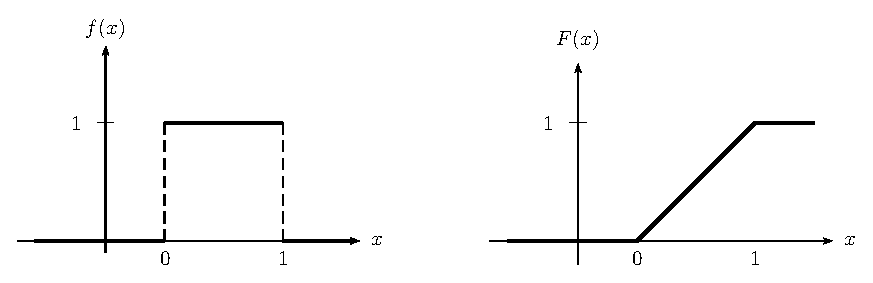
\includegraphics{pstricks/unif01fF}
\caption{$f(x)$ and $F(x)$ of the $\uniform(0,1)$ random variable $X$.}
\end{center}
\end{figure}

\begin{figure}[htpb]
\caption{A convenient but mathematically imprecise Matlab plot from a polyline interpolation for the PDF and DF or CDF of the $\uniform(0,1)$ continuous RV $X$.\label{F:unif01}}
\centering   \makebox{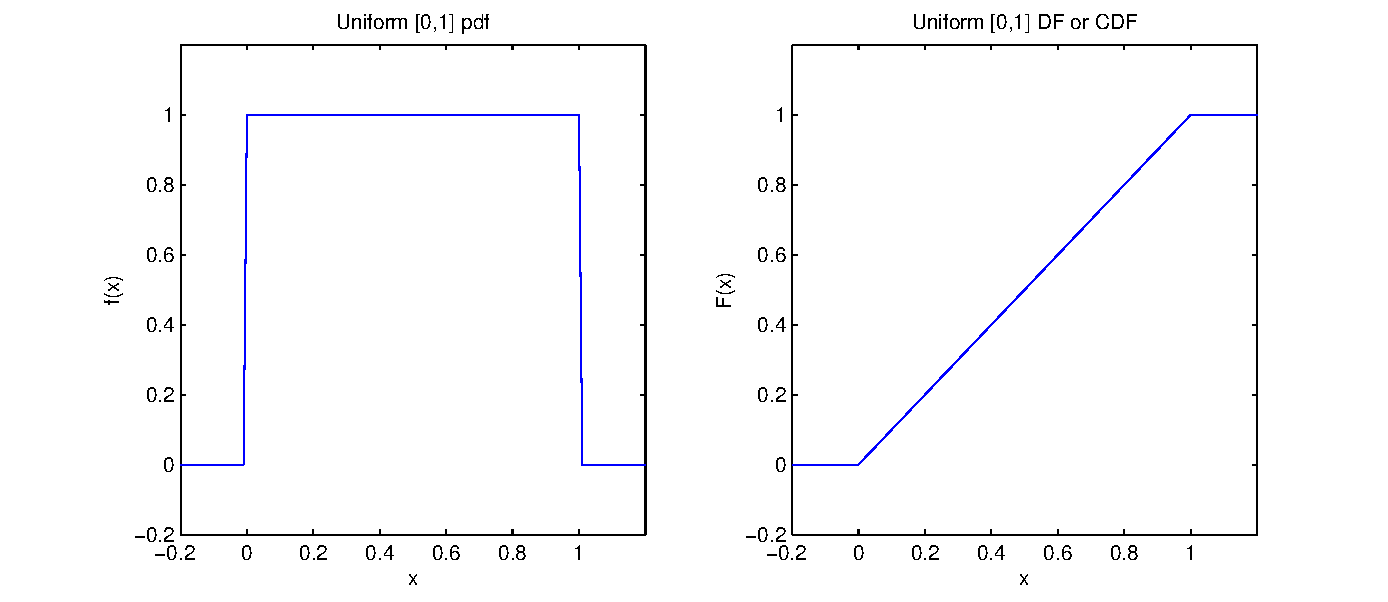
\includegraphics[width=4.5in]{figures/Unif01pdfcdf}}
\end{figure}

\remove{
\begin{labwork}[PDF of $\uniform(0,1)$ RV]\label{LW:Unif01Pdf}
Let us encode the PDF of $\uniform(0,1)$ as an M-file in {\sc Matlab}.  Notice that the PDF function assigns $1$ to every value of $x \in [0,1]$ and $0$ to every value of $x \notin [0,1]$.  So, the problem mostly boils down to finding the entries inside and outside the range.  We can use {\sc Matlab}'s built-in {\tt find} function for this purpose.  We give an example to illustrate the syntax of {\tt find}.
\begin{VrbM}
>> Xs=[0.2511    1.6160    0.4733    -5.3517    0.8308    0.5853    2.5497] % an array Xs with real values 
Xs =    0.2511    1.6160    0.4733   -5.3517    0.8308    0.5853    2.5497
\end{VrbM}
We can obtain the indices of {\tt Xs} whose values are $\geq 0$, i.e.~$\{i: {\tt Xs}(i) \geq 0 \}$ and the indices of {\tt Xs} whose values are $\leq 1$, i.e.~$\{i: {\tt Xs}(i) \leq 1 \}$ as follows:
\begin{VrbM}
>> find(Xs >= 0)
ans =     1     2     3     5     6     7
>> find(Xs <= 1)
ans =     1     3     4     5     6
\end{VrbM}
The intersection of the two sets of indices, i.e.~$\{i: {\tt Xs}(i) \geq 0 \ \text{ and } \  {\tt Xs}(i) \leq 1 \} = \{i: 0 \leq {\tt Xs}(i) \leq 1 \}$ can be obtained by {\tt \&}, the Boolean and, as follows:
\begin{VrbM}
>> find(Xs >= 0 & Xs <= 1)
ans =     1     3     5     6
\end{VrbM}
Finally, we know which indices of the {\tt Xs} array should have the PDF value of $1$.  The remaining indices of {\tt Xs} should therefore have the PDF value of $0$.  Let us declare an array called {\tt Pdf} for the PDF values corresponding to the {\tt Xs}.  We can initialise this array with zeros using the {\tt zeros} function and make it of the same size as {\tt Xs} as follows:
\begin{VrbM}
>> size(Xs)
ans =     1     7
>> Pdf = zeros(1,7)
Pdf =     0     0     0     0     0     0     0
\end{VrbM}
Now, we can set the indices $1,3,5,6$ (returned by {\tt find(Xs >= 0 \& Xs <= 1)}) of {\tt Pdf} array to 1.
\begin{VrbM}
>> Pdf([1     3     5     6])=1
Pdf =     1     0     1     0     1     1     0
\end{VrbM}
We can modularise this process for an arbitrary input array {\tt x} via a function in the following M-file.
\VrbMf[label=Unif01Pdf.m]{scripts/Unif01Pdf.m} 
Let us call the function we wrote called {\tt Unif01Pdf} next.
\begin{VrbM}
>> help Unif01Pdf
  Unif01Pdf(x) returns the PDF of Uniform(0,1) RV X
  the input x can be an array
>> Xs
Xs =    0.2511    1.6160    0.4733   -5.3517    0.8308    0.5853    2.5497
>> Unif01Pdf(Xs)
ans =     1     0     1     0     1     1     0
\end{VrbM}
\end{labwork}

\begin{labwork}[CDF of $\uniform(0,1)$ RV]\label{LW:Unif01Cdf}
Understand each step in the function {\tt Unif01Cdf}:
\VrbMf[label=Unif01Cdf.m]{scripts/Unif01Cdf.m} 
When we type in {\tt help Unif01Cdf}, {\tt Xs} and {\tt Unif01Cdf(Xs)} we can confirm that the {\tt Unif01Cdf} function is correctly reporting the CDF values of the input array {\tt Xs}.
\begin{VrbM}
>> help Unif01Cdf
  Unif01Cdf(x) returns the CDF of Uniform(0,1) RV X
  the input x can be an array 
>> Xs
Xs =    0.2511    1.6160    0.4733   -5.3517    0.8308    0.5853    2.5497
>> Unif01Cdf(Xs)
ans =    0.2511    1.0000    0.4733         0    0.8308    0.5853    1.0000
\end{VrbM}
\end{labwork}

\begin{labwork}[Plot of the PDF and the CDF for the $\uniform(0,1)$ RV]\label{LW:PlotUnif01PdfCdf}
Generate the plot of the PDF and the CDF for the $\uniform(0,1)$ RV $X$ by following the commands below.  Go through every step and understand each command when you reproduce the plot.
\VrbMf[label=plotunif.m]{scripts/plotunif.m} 
The plot was saved as an encapsulated postscript file from the File menu of the Figure window and is displayed in \hyperref[F:unif01]{Figure~\ref*{F:unif01}}.
 \end{labwork}
}

{\bf **tossing a fair coin infinitely often, i.e., IID sequence of $\bernoulli(1/2)$ trials, and the fundamental model}

%TODO\input{figures/UnifsInUnif.tex}

--- The fundamental model is equivalent to infinite tosses of a fair coin (see using binary expansion of any $x \in (0,1)$ if you want as suggested in optional Exercise~\ref{underMPSA} on intuiting a most primitive sigma-algebra)

--- The fundamental model has infinitely many copies of itself within it! You can see this since its DF $F$ is the identity function on $[0,1]$ or equivalently how the dyadic binary tree is identical below a given node in the tree no matter which node in the tree you choose.


{\bf **universality of the fundamental model}

--- one can obtain any other random variable from the fundamental model whose unique DF is its own inverse, i.e., $F(x)=F^{[-1]}(x)$, as you will See from von Neumann's Fundamental Theorem of Simulation in Chapter~\ref{S:RNG}.

\subsection{Some Common Continuous Random Variables}\label{S:CommonContRV}

Let us warm-up with an example.


\begin{example}\label{EgPdfeToTheminusx}
{Let $X$ have  density function $f(x)\,=\,e^{-x}$, if $x\geq0$,  and
  zero otherwise.
  \be
\item[(a)]Find the distribution function.
\item[(b)] Find the probabilities, $P(\frac{1}{4}\leq X \leq 2)$ and
  $P\left(-\frac{1}{2}\leq X\leq \frac{1}{2}\right)$.
\item[(c)]Find $x$ such that $P(X\leq x) =0.95$.
\ee
}

Solution:\\[4pt]
{\be
\item[(a)] 
$$
F(x)\;=\;\int_0^{x}e^{-v}dv
\;=\;\left.-e^{-v}\right]^x_0 
\;=\;-e^{-x}+1\;=\;1-e^{-x}\qquad \textrm{if }x \geq 0
$$
Therefore, 
$$
F(x)\;=\;
\begin{cases}
1-e^{-x}& \textrm{if }x \geq 0\enspace , \\
0&\textrm{otherwise}\enspace.
\end{cases}
$$
\item[(b)]
$$
P\left(\frac{1}{4}\leq X\leq 2\right) 
\;=\;F(2)-\,F\left(\frac{1}{4}\right)
\;=\;0.634\;\;(\text{3 sig. fig.})
$$
$$
P\left(-\frac{1}{2}\leq X\leq \frac{1}{2}\right) 
\;=\;
F\left(\frac{1}{2}\right)\,-\,F\left(-\frac{1}{2}\right)
\;=\;0.394 \;\;(\text{3 sig. fig.})
$$
\item[(c)] $$P(X\leq x)\;=\;F(x)\;=\;1-e^{-x}\;=\;0.95$$
Therefore, $$x\;=\;-\log(1-0.95)\;=\;3.00\;\;(\text{3 sig. fig.})\enspace.$$
\ee
}
\end{example}

\begin{figure}[htbp]
\begin{center}
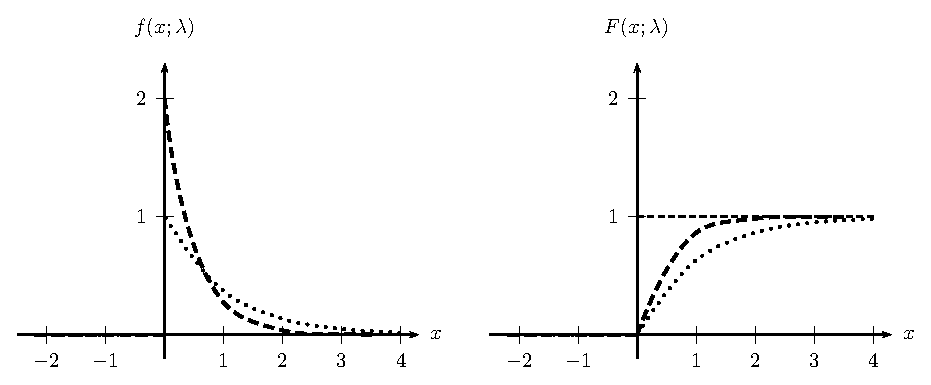
\includegraphics[width=5.0in]{pstricks/exponentialLambdafF}
\caption{$f(x;\lambda)$ and $F(x;\lambda)$ of an exponential random variable where $\lambda=1$ (dotted) and $\lambda=2$ (dashed).}
\end{center}
\end{figure}


The previous example is a special case of the following parametric
family of random variables.

\begin{model}[$\exponential(\lambda)$]\label{M:exponential}
For a given $\lambda > 0$, an $\exponential(\lambda)$ RV has the following PDF $f$ and DF $F$ and its complementary distribution function denoted by $\overline{F}(x; \lambda) := \p(X > x) = 1-F(x;\lambda)$:
\begin{eqnarray}\label{E:Exponentialpdfcdf}
f(x; \lambda) &=& \BB{1}_{(0,\infty)} \lambda e^{-\lambda x} =
\begin{cases}
\lambda \exp(-\lambda x) & x>0 \enspace ,\\
0&\textrm{otherwise} \enspace ,
\end{cases}\\
F(x; \lambda) &=& 1-e^{-\lambda x} \enspace ,\\ 
\overline{F}(x; \lambda) = e^{-\lambda x} \enspace .
\end{eqnarray}

The last two equations are derived from definitions as follows:
\begin{multline*}
F(x; \lambda) = \int_{-\infty}^{x} \BB{1}_{(0,\infty)} \lambda e^{-\lambda v} dv = \lambda \int_0^x e^{-\lambda v} dv = \lambda \left( -\frac{1}{\lambda} e^{-\lambda v} \right]_0^x =  \left( - e^{-\lambda v} \right]_0^x \\ \notag
= -e^{-\lambda x} - (-e^{-0}) = -e^{-\lambda x} - (-1/e^0) = -e^{-\lambda x} - (-1/1) = -e^{-\lambda x} - (-1) = -e^{-\lambda x} + 1 \\ \notag
\end{multline*}
\[\p(X > x) = 1- \p(X \leq x) = 1- F(x; \lambda) = 1 - \left( 1-e^{-\lambda x}\right) = e^{-\lambda x}\].

This distribution is unique because of its property of {\bf memorylessness}, i.e., $\p(X>x+y | X > y) = e^{-\lambda x}$, and plays a fundamental role in modeling continuous time processes, such as time between occurrence of events of interest, as we will see in the sequel.
\end{model}

\remove{%%%%%%%%%%%%%%% SIMUL
We encode the PDF and DF of the $\exponential(\lambda)$ RV as \Matlab functions {\tt ExponentialPdf} and {\tt ExponentialCdf} and use them to produce \hyperref[F:plotPdfCdfExponentials]{Figure~\ref*{F:plotPdfCdfExponentials}} in \hyperref[Mf:ExponentialPdfCdf]{Labwork~\ref*{Mf:ExponentialPdfCdf}}.
}%end remove%%%%%%%%%%%%%%%% SIMUL?

\begin{figure}[htpb]
\caption{Density and distribution functions of $\exponential(\lambda)$ RVs, for $\lambda=1, 10, 10^{-1}$, in four different axes scales.\label{F:plotPdfCdfExponentials}}
\centering   \makebox{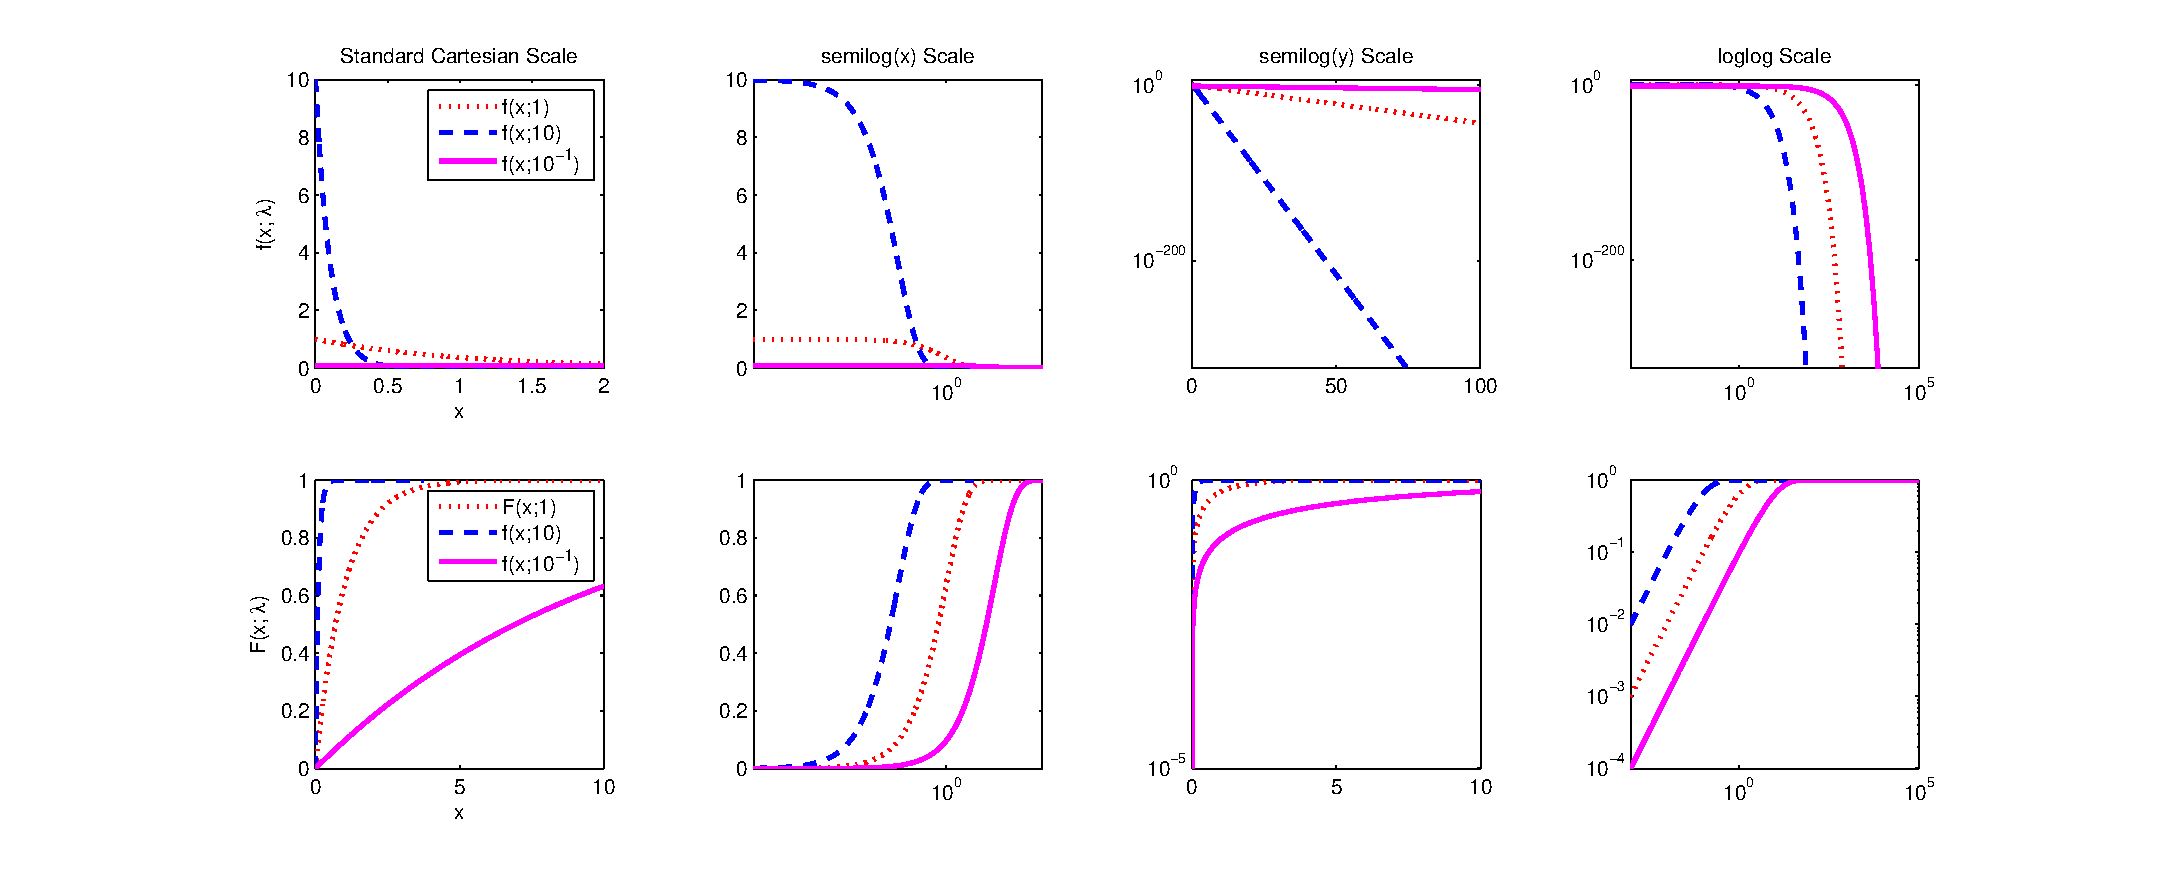
\includegraphics[width=6.5in]{figures/plotPdfCdfExponentials}}
\end{figure}

\begin{example}[On a dark desert highway]\label{darkDesHWWaitingTime}
{At a certain location on a dark desert highway, the time in minutes between arrival of cars that exceed the speed limit is an $\exponential(\lambda=1/60)$ random variable. 
If you just saw a car that exceeded the speed limit then what is the probability of waiting less than 5 minutes before seeing another car that will exceed the speed limit?}

{\em Solution:}\\[4pt]
{
The waiting time in minutes is simply given by the $\exponential(\lambda=1/60)$ random variable.  
Thus, the desired probability is 
\[
P(0 \leq X < 5)
\;=\;\int_0^5\frac{1}{60}e^{-\frac{1}{60}x}dx
\;=\;\left.-e^{-\frac{1}{60}x}\right]_0^5
\;=\;-e^{-\frac{1}{12}}\,+\,1\;\approx\; 0.07996.
\]
In exam you can stop at the expression $-e^{-\frac{1}{12}}+1$ for full credit.  
You may need a calculator for the last step (with answer $0.07996$).

Note: We could use the distribution function directly:
\[P(0 \leq X < 5)\;=\;  F\left(5; \frac{1}{60}\right) \,-\, F\left(0;\frac{1}{60}\right) \;=\;
F\left(5;\frac{1}{60}\right) \;=\; 1-e^{-\frac{1}{60}5} \;=\; 1--e^{-\frac{1}{12}} \;\approx\; 0.07996\]
}
\end{example}

\begin{prop}[Memorylessness of $\exponential(\lambda)$ RV]\label{P:memorylessnessOfExponentialLambdaRV}
If $X \sim \exponential(\lambda)$, then $X$ has the property of {\bf memorylessness}, i.e., 
\begin{equation}
\boxed
{
\p(X>x+y  | X > y) = \p (X > x) \enspace .
} 
\end{equation}
\end{prop}
\begin{proof}
By the definition of conditional probability,
\[
\p(X > x+y | X > y) =\p( \{X>x+y\} |  \{X > y \}) = \frac{\p( \{X>x+y\} \cap \{X > y \})}{\p( \{X>y\} )}
\]
Due to redundancy, i.e., $\{X>x+y\} \subset \{X > y \} \implies \{X>x+y\} \cap \{X > y \}=\{X>x+y\}$, so
\begin{align*}
\p(X > x+y | X > y) 
&=  \frac{\p( \{X>x+y\}}{\p( \{X>y\} )} = \frac{\overline{F}(x+y; \lambda)}{\overline{F}(y; \lambda)} = \frac{e^{-\lambda(x+y)}}{e^{-\lambda y}} 
= \frac{e^{-\lambda x} e^{-\lambda y}}{e^{-\lambda y}}
= e^{-\lambda x} = \overline{F}(x; \lambda) \\
&= \p(X > x)
\end{align*}
\end{proof}

\begin{Exercise}[title={Memoryless Server Times},label={xmemorylessnessOfExponentialLambdaRV}]
Suppose customers in a Queue are served one at a time by a server whose service time is an independent and identical $\exponential(\lambda)$ RV, with $\lambda=1/10$. The server is immediately free to serve the next customer once the current customer being served is done.
Suppose you just arrive and are the first in the queue and know that the server is busy serving another customer. You do not know how long the customer has already been in service. 
What is the probability that the server will be free after $2$ units of time?
\end{Exercise}
\begin{Answer}
Let $X \sim \exponential(\lambda=0.1)$ denote the time taken to serve any given customer in an IID manner.
Let $y$ denote the unknown time that the current customer being served has already been served before your arrival.
By memorylessness of $\exponential(\lambda=0.1)$ RV $X$, we know $\p(X > 2 + y | X > y) = \p(X > 2) = e^{-\lambda 2} = e^{-2/10}$.
\end{Answer}

\bigskip

Let us introduce parameters for the lower and upper bounds of the interval upon which a continuous RV is uniformly distributed using the following probability model.
 
\begin{model}[$\uniform(\theta_1,\theta_2)$]\label{M:Uniformab}
Given two real parameters $\theta_1,\theta_2 \in \Rz$, such that $\theta_1 < \theta_2$, the PDF of the $Uniform(\theta_1,\theta_2)$ RV $X$ is:
\begin{equation}\label{E:Uniformabpdf}
f(x;\theta_1,\theta_2) =
\begin{cases}
\frac{1}{\theta_2 - \theta_1} & \text{if $\theta_1 \leq x \leq \theta_2$,}\\
0 & \text{otherwise}
\end{cases}
\end{equation}
and its DF given by $F(x;\theta_1,\theta_2) = \int_{- \infty}^x f(y; \theta_1,\theta_2) \, dy$ is:
\begin{equation}\label{E:Uniformabcdf}
F(x; \theta_1,\theta_2) =
\begin{cases}
0 & \text{if $x < \theta_1$} \\
\frac{x-\theta_1}{\theta_2-\theta_1} & if~\theta_1 \leq x \leq \theta_2,\\
1 & \text{if $x > \theta_2$}
\end{cases}
\end{equation}
Recall that we emphasise the dependence of the probabilities on the two parameters $\theta_1$ and $\theta_2$ by specifying them following the semicolon in the argument for $f$ and $F$.
\end{model}

\begin{figure}[htbp]
\begin{center}
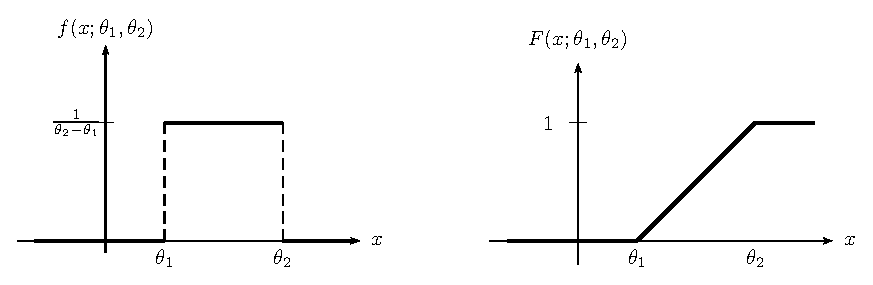
\includegraphics{pstricks/uniftheta1theta2fF}
\caption{$f(x)$ and $F(x)$ of the $\uniform(\theta_1,\theta_2)$ random variable $X$.}
\end{center}
\end{figure}


\begin{Exercise}\label{xPDFHeightOfUniformOn2_6}
{Consider  a random variable with a probability density function
\[f(x)\;=\;\begin{cases}\displaystyle k & \textrm{if} \qquad  2\leq
  x\leq 6 \enspace,\\0& \text{otherwise}
\end{cases}
\]
\be
\item[(a)] Find the value of $k$.
\item[(b)] Sketch the graphs of $f(x)$ and $F(x)$.
\ee
}
\end{Exercise}

\begin{Answer}
{\be
\item[(a)] Since $f(x)$ is a density function which integrates to one,
\ba{\int^6_2  f(x) \,dx &\;=\; \int^6_2  k \, dx\\[3pt]
1  &\;=\;\left.  kx \right]^6_2\\[3pt]
1  &\;=\;6k \,-\, 2k\\[3pt]
1  &\;=\;4k\\[3pt]
k&\;=\; \frac{1}{4}
}
as expected!

\medskip

\item[(b)] Now $$F(x)\;=\;\begin{cases}0& x< 2 \\
\frac{1}{4} \,( x-2)  & 2\leq x<6\\
1& x\geq 6\enspace.
\end{cases}
$$
so the graphs are:

\cen{Graphs of $f(x)$ and $F(x)$.}
\begin{center}
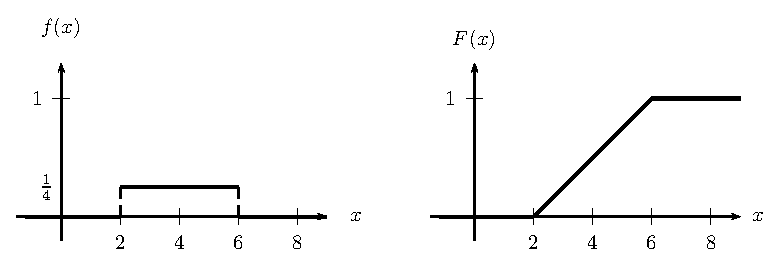
\includegraphics{pstricks/unif26fF}
\end{center}

\ee
}
\end{Answer}
%\remove{%%%%%%%%%%%%%%%% drawn by hand
%\begin{figure}[htpb]
%\caption{A plot of the PDF, DF and inverse DF of the $\uniform(-1,1)$ RV $X$.\label{F:unifpm1}}
%\centering   \makebox{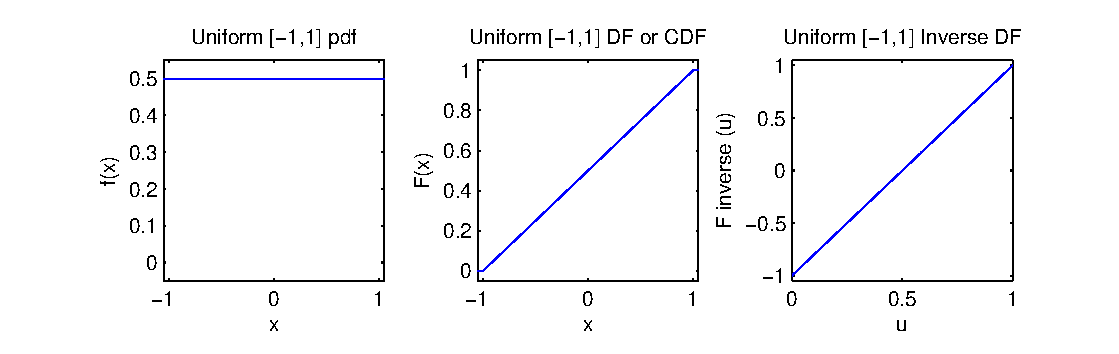
\includegraphics[width=6.5in]{figures/Unifpm1pdfcdf}}
%\end{figure}
%}%%%%%%%%%%%%% SHOULD go with Simulation?

The standard normal distribution is the most important continuous
probability distribution. It was first described by De Moivre in 1733
and subsequently by C.~F.~Gauss (1777 - 1885).
Many  random variables  have a normal distribution, or they are
approximately normal, or can be transformed into normal random variables
in a relatively simple fashion. Furthermore, the normal distribution is
a useful approximation of more complicated distributions.
%%%%Location-scale Gaussian family as a linear transformation of the standard Gaussian RV

\begin{framed}
\begin{model}[$\normal(0,1)$ or standard normal or Gaussian RV]\label{Df:StandardNormal} 
A continuous random variable $Z$ is called \textbf{standard normal} or {\bf standard Gaussian} 
if its probability density function is
\begin{equation}\label{E:StandardNormalPdf}
\phi(z) = \frac{1}{\sqrt{2\pi}} \exp{\left( -\frac{z^2}{2}\right)} \enspace.
\end{equation}
\end{model}
\end{framed}

An exercise in calculus yields the first two derivatives of $\phi$ as follows:
\[
\frac{d \phi}{dz} = - \frac{1}{\sqrt{2\pi}}z \exp{\left( -\frac{z^2}{2}\right)}=-z\phi(z), \quad
\frac{d^2 \phi}{dz^2} = \frac{1}{\sqrt{2\pi}}(z^2-1) \exp{\left(-\frac{z^2}{2} \right)}=(z^2-1)\phi(z) \enspace .
\]
Thus, $\phi$ has a global maximum at $0$, it is concave down if $z \in (-1,1)$ and concave up if $z \in (-\infty,-1) \cup (1,\infty)$.  
This shows that the graph of $\phi$ is shaped like a smooth symmetric bell centred at the origin over the real line.


\begin{classwork}\label{xDrawPDFOfStdNormal}
From the above exercise in calculus let us draw the graph of $\phi$ by hand now!

Do it step by step: $z^2$, $-z^2$, $-z^2/2$, $\exp(-z^2/2)$, $\phi(z) = \frac{1}{\sqrt{2\pi}} \exp(-z^2/2)$ now! 
\vspace*{20mm}
\end{classwork}

The distribution function of $Z$ is given by
\begin{equation}\label{E:StandardNormalDF}
\Phi(z) \;=\;\frac{1}{\sqrt{2\pi}}\int^z_{-\infty}e^{-v^2/2}\;dv \enspace .
\end{equation}

\begin{rem}
{The integral for $\Phi(z)$ has no closed form expression and cannot be evaluated exactly by standard methods of calculus, but its values can be
obtained numerically and tabulated.  Values of $\Phi(z)$ are tabulated in the ``Standard Normal Distribution Function Table'' in Sec.~\ref{S:NormalDFTable}.}

We can express $\Phi(z)$ %$F(x;\mu,\sigma^2)$ 
in terms of the error function ($\erf$) as follows:
\begin{equation}\label{E:DFStandardNormalviaErf}
%F(x;\mu,\sigma^2) = \frac{1}{2} \ \erf \left(  \frac{x-\mu}{\sqrt{2 \sigma^2}} \right)+ \frac{1}{2}
\Phi(z) = \frac{1}{2} \ \erf \left(  \frac{z}{\sqrt{2}} \right)+ \frac{1}{2}
\end{equation}
And use \Matlab's \texttt{erf} function to get $\Phi(z)$ numerically instead of looking up the Table.
\end{rem}

\begin{classwork}\label{xDrawDFOfStdNormal}
{Note that the curve of $\Phi(z)$ is $S$-shaped, increasing in a strictly monotone way from $0$ at $-\infty$ to $1$ at $\infty$, and intersects the vertical axis at $1/2$. Draw this by hand too.}\\[4pt]
just do it! \vspace*{20mm}
\end{classwork}

\begin{example}\label{Eg:UsingNormalTables}
Find the probabilities, using  normal tables,  that a random variable having the standard
  normal distribution will take on a value:
\bcols{2}\begin{itemize}
\item [(a)] less that 1.72
\item [(b)]less than -0.88
\item [(c)]between 1.30 and 1.75
\item [(d)] between -0.25 and 0.45
\end{itemize}\ecols
\begin{itemize}
 \item [(a)]
$$P(Z<1.72)\;=\;\Phi(1.72) \;=\; 0.9573$$
 \item [(b)] First note that $P(Z<0.88)\;=\;0.8106$, so that
   \ba{P(Z<-0.88) & \;=\;P(Z>0.88) \\
     &\;=\;1-P(Z<0.88)\\&\;=\;1-\Phi(0.88)\\ &\;=\;1-0.8106\;=\;0.1894}
 \item [(c)]
$P(1.30<Z<1.75)\;=\;\Phi(1.75)-\Phi(1.30)\;=\;0.9599-0.9032\;=\;0.0567$
 \item [(d)]
\ba{P(-0.25<Z<0.45)&\;=\;P(Z<0.45)-P(Z<-0.25)\\&\;=\;P(Z<0.45)-(1-P(Z<0.25))\\&\;=\;\Phi(0.45)-(1-\Phi(0.25)) \\&=\;(0.6736)-(1-0.5987)\\&\;=\;0.2723}
\end{itemize}
\end{example}
%%%%%%%%%%%%%%%%%%%%%%%%%%%%%%%%%%%%%%%%%%%%%%%%%%%%%%%%%%%%%%%%
\bigskip
{
\begin{framed}
CONTINUOUS RANDOM VARIABLES: NOTATION\\

$f(x)$: Probability density function (PDF)
\begin{itemize}
\item$f(x)\;\geq\;0$
\item Areas underneath $f(x)$ measure probabilities.
\end{itemize}

$F(x)$: Distribution function (DF)
\begin{itemize}
\item $0\;\leq\;\ F(x)\;\leq \;1$
\item $F(x)\;= \;P(X\leq x)$ is a probability
\item $F^{\prime}(x)\;=\;f(x)$ for every $x$ where $f(x)$ is continuous
\item $F(x)\;=\;\displaystyle\int^x_{-\infty}f(v)dv$
\item $P(a<X\leq b)\;=\;F(b)-F(a)\;=\;\displaystyle \int^b_af(v)dv$
\end{itemize}
\end{framed}
}


\remove{
%The $\exponential(\lambda)$ random variable gives  the waiting times\emph{ between} successive events of a process where the number of events in unit time is a $\poisson(\lambda)$  random variable.
%Ben wants this justified - will do in MATH103 next year...
\Exmp
}

\section{Exercises in Continuous Random Variables}\label{S:xsContinuousRVs}
\begin{ExerciseList}
\Exercise
Consider the probability density function
$$f(x)\;=\;\begin{cases} k &-4 \leq x\leq4\\0&\textrm{otherwise}\end{cases}\,.$$

\be
\item Find  the value of $k$.
\item Find the distribution function, $F$.
\item   Graph $f$ and  $F$.
\ee
\Answer
\be
\item Since $f(x)$ is a (continuous) probability density function which integrates to one,
$$\int_{-4}^4kdx\;=\;1\,.$$
That is, 
\ba{k \,x\bigg]^4_{-4}&=\;1\\[3pt]k(4-(-4))&=\;1\\[3pt]8k&=\;1\\[3pt]k&=\;\frac{1}{8}}

\item First note that if $x <  -4$, then  $$F(x)\;=\;\int^x_{-\infty}0\,dv\;=\;0\,.$$
If $-4 \leq x \leq 4$, then
\begin{align*}F(x)&=\;\int^{-4}_{-\infty}0\,dv\;+\;\int^x_{-4} \frac{1}{8}\,dv\\[3pt]
&=\;0\;+\;\left[ \frac{1}{8}\, v \right]^x_{-4}\\[3pt]
&=\;  \frac{1}{8} (x +4)\end{align*}
If $x\geq 4$, then
\begin{align*}F(x)&=\int^{-4}_{-\infty}0\,dv\;+\;\int^{4}_{-4}
  \frac{1}{8} \,dv\;+\;\int^x_{4} 0 \,dv\\[3pt]
&=0\;+\;\left[\frac{1}{8} v \right]^4_{-4}\;+\;0\\[3pt]
&=\; 1\end{align*}
Hence  $$F(x)\;=\;\begin{cases}0&x <  -4\\ \frac{1}{8} (x+4) &-4 \leq
  x\leq 4\\1&x\geq 4\end{cases}$$

\item  The graphs of $f(x)$ and $F(x)$ for  random variable $X$ are as follows:
%TODO\centering   \makebox{\includegraphics[width=6.5in]{figures/fandFforConstantDensity.png}}

\ee

\Exercise
Assume that a new light bulb will burn out at time $t$ hours according to the probability density function given by 
$$
f(t)\;=\;
\begin{cases}
\lambda e^{-\lambda t} & \text{ if } t >0 \enspace,\\
0 & \text{ otherwise} \enspace .
\end{cases}
$$
In this context, $\lambda$ is often called the failure rate of the bulb.

\be
\item[(a)]Assume that $\lambda=0.01$, and find the probability that the
  bulb will not burn out before $\tau$ hours. This $\tau$-specific probability is often
  called the reliability of the bulb.

Hint: Use the distribution function for an $\exponential(\lambda)$ random variable (recall, $F(\tau;\lambda)=\int_{-\infty}^{\tau} f(t) dt$)!

\item[(b)]For what  value of $\tau$ is the reliability of the bulb exactly $\frac{1}{2}$?
\ee
\Answer
\be
\item Since the distribution function is $F(t; \lambda) \,=\,
  1 - \exp( - \lambda t)$,
 \[\P(t>\tau)\;=\;1-\P(t<\tau)\;=\; 1 - F(\tau;\lambda=0.01) \;=\;1-(1-e^{-0.01\tau})\;=\;e^{-0.01\tau}\,.\]

\item Set  \[\P(t>\tau)\;=\;e^{-0.01\tau}\;=\;\frac{1}{2}\]
and solve for $\tau$ to get  then $\tau\,=\,-100\times \log(0.5)\,=\,69.3\quad (\text{3 sig. fig.})$\,.
\ee

\Exercise 
Let the random variable $X$ be the time  after which certain ball bearings wear out, with density
$$f(x)\;=\;\begin{cases} ke^{-x}&0\leq x\leq 2\\0&\textrm{otherwise}\end{cases}\enspace.$$
Note: $X$ is measured in  years.
\be
\item Find $k$.
\item Find the probability that a bearing will last at least 1 year.
\ee
\Answer
\be
\item

\ba{\int^2_0 k\,e^{-x}\,dx &=\;1\\[3pt]
\left[ -k\,e^{-x}\right]^2_0&=\;1\\[3pt]
k\,(-e^{-2}+1)&=\;1\\[3pt]
k&=\;\frac{1}{1-e^{-2}} \quad (\approx 1.1565)
}

\item
\ba{\P(X\geq1)&=1\,-\,\P(X<1)\\[3pt]
&=\;1\;-\;\int^1_0 k e^{-x}\,dx\\[3pt]
&=\;1\;+\;k\left(e^{-x}\right]^1_0\\[3pt]
&=\;1\;+\;\frac{e^{-1}-1}{1-e^{-2}}\\[3pt]
&\approx\;0.2689}

\ee


\end{ExerciseList}



\section{Transformations of random variables}\label{S:TransformationsOFRvs}

Suppose we know the distribution of a random variable $X$.  How do we find the distribution of a transformation of $X$, say $g(X)$?
Before we answer this question let us ask a motivational question.  Why are we interested in functions of random variables?

\begin{example}\label{EgProfitOn5With500cost}
Consider a simple financial example where an individual sells $X$ items per day, the profit per item is $\$ 5$ and the overhead costs are $\$ 500$ per day.  The original random variable is $X$, but the random variable $Y$ which gives the daily profit is of more interest, where
\[
Y = 5X - 500 \enspace . 
\]
\end{example}


\begin{example}\label{EgSignal2NoiseInDecibels10TimeslogBase10OfX}
In a cell-phone system a mobile signal may have a signal-to-noise-ratio of $X$, but engineers prefer to express such ratios in decibels, i.e.,
\[
Y = 10 \log_{10}(X) \enspace .
\]
\end{example}

\subsection{A Review of Inverse Images}\label{S:RWInverseImages}
Hence in a great many situations we are more interested in functions of random variables. 
Let us return to our original question of determining the distribution of a transformation or function of $X$.  
First note that this transformation of $X$ is itself another random variable, say $Y = g(X)$, 
where $g$ is a function from a subset $\mathbb{X}$ of $\mathbb{R}$ to a subset $\mathbb{Y}$ of $\mathbb{R}$, 
i.e., $g: \mathbb{X} \to \mathbb{Y}$, $\mathbb{X} \subset \mathbb{R}$ and $\mathbb{Y} \subset \mathbb{R}$.

The {\bf inverse image} of a set $A$ is the set of all real numbers in $\mathbb{X}$ whose image is in $A$, i.e.,
\[
g^{[-1]}(A) = \{x \in \mathbb{X} : g(x) \in A \} \enspace .
\] 
In other words,
\[
x \in g^{[-1]}(A) \ \text{if and only if} \ g(x) \in A \enspace .
\]
For example,
\begin{itemize}
\item if $g(x)=2x$ then $g^{[-1]}([4,6])=[2,3]$
\item if $g(x)=2x+1$ then $g^{[-1]}([5,7])=[2,3]$
\item if $g(x)=x^3$ then $g^{[-1]}([1,8])=[1,2]$
\item if $g(x)=x^2$ then $g^{[-1]}([1,4])=[-2,-1] \cup [1,2]$
\item if $g(x)=\sin(x)$ then $g^{[-1]}([-1,1])=\mathbb{R}$
\item if ... %Raaz add other examples of the transformations done in the sequel here
\end{itemize}
For the singleton set $A = \{y\}$, we write $g^{[-1]}(y)$ instead of $g^{[-1]}(\{y\})$.  
For example,
\begin{itemize}
\item if $g(x)=2x$ then $g^{[-1]}(4)=\{2\}$
\item if $g(x)=2x+1$ then $g^{[-1]}(7)=\{3\}$
\item if $g(x)=x^3$ then $g^{[-1]}(8)=\{2\}$
\item if $g(x)=x^2$ then $g^{[-1]}(4)=\{-2,2\}$
\item if $g(x)=\sin(x)$ then $g^{[-1]}(0)=\{k \pi: k \in \mathbb{Z}\} = \{\ldots, -3 \pi, -2 \pi, -\pi,0,\pi, 2\pi,3\pi, \ldots\}$
\item if ... %Raaz add other examples of the transformations done in the sequel here
\end{itemize}
If $g:\mathbb{X}\to\mathbb{Y}$ is one-to-one (injective) and onto (surjective), then the inverse image of a singleton set is itself a singleton set.  
Thus, the inverse image of such a function $g$ becomes itself a function and is called the {\bf inverse function}.
One can find the inverse function, if it exists by the following steps:
\begin{itemize}
\item[{\sf Step 1;}] write $y=g(x)$
\item[{\sf Step 2;}] solve for $x$ in terms of $y$
\item[{\sf Step 3;}] set $g^{-1}(y)$ to be this solution
\end{itemize}
We write $g^{-1}$ whenever the inverse image $g^{[-1]}$ exists as an inverse function of $g$.  
Thus, the inverse function $g^{-1}$ is a specific type of inverse image $g^{[-1]}$.  
For example,
\begin{itemize}
\item if $g(x)=2x$ then $g:\mathbb{R} \to \mathbb{R}$ is injective and surjective and therefore its inverse function is:\\
{\sf Step 1;} $y=2x$, {\sf Step 2;} $x=\frac{y}{2}$, {\sf Step 3;} $g^{-1}(y)=\frac{y}{2}$
\item if $g(x)=2x+1$ then $g:\mathbb{R} \to \mathbb{R}$ is injective and surjective and therefore its inverse function is:\\
{\sf Step 1;} $y=2x+1$, {\sf Step 2;} $x=\frac{y-1}{2}$, {\sf Step 3;} $g^{-1}(y)=\frac{y-1}{2}$
\item if $g(x)=x^3$ then $g:\mathbb{R} \to \mathbb{R}$ is injective and surjective and therefore its inverse function is:\\
{\sf Step 1;} $y=x^3$, {\sf Step 2;} $x={y}^{\frac{1}{3}}$, {\sf Step 3;} $g^{-1}(y)={y}^{\frac{1}{3}}$
\end{itemize}
However, you need to be careful by limiting the domain to obtain the inverse function for the following examples:
\begin{itemize}
\item if $g(x)=x^2$ and domain of $g$ is $[0,+\infty)$ then its inverse function is $g^{-1}(y)=\sqrt{y}$, 
i.e., if $g(x)=x^2 : [0,+\infty) \to [0,+\infty)$ then the inverse image $g^{[-1]}(y)$ for $y \in [0,+\infty)$ is given by the inverse function $g^{-1}(y)=\sqrt{y} : [0,+\infty) \to [0,+\infty)$.
\item if $g(x)=x^2$ and domain of $g$ is $(-\infty,0]$ then its inverse function is $g^{-1}(y)=-\sqrt{y}$, 
i.e., if $g(x)=x^2 : (-\infty,0] \to [0,+\infty)$ then the inverse image $g^{[-1]}(y)$ for $y \in [0,+\infty)$ is given by the inverse function $g^{-1}(y)=-\sqrt{y} : [0,+\infty) \to (-\infty,0]$.
\item if $g(x)=\sin(x)$ and domain of $g$ is $[0,\frac{\pi}{2}]$ then its inverse function $g^{-1}(y)=\arcsin(y)$, i.e., if $g(x)=\sin(x) : [0,\frac{\pi}{2}] \to [0,1]$ then the inverse image $g^{[-1]}(y)$ for $y \in [0,1]$ is given by the inverse function $g^{-1}(y)=\arcsin(y) : [0,1] \to [0, \frac{\pi}{2}]$.
\item if $g(x)=\sin(x)$ and domain of $g$ is $[-\frac{\pi}{2},\frac{\pi}{2}]$ then its inverse function $g^{-1}(y)=\arcsin(y)$, i.e., if $g(x)=\sin(x) : [-\frac{\pi}{2},\frac{\pi}{2}] \to [-1,1]$ then the inverse image $g^{[-1]}(y)$ for $y \in [-1,1]$ is given by the inverse function $g^{-1}(y)=\arcsin(y) : [-1,1] \to [-\frac{\pi}{2},\frac{\pi}{2}]$.
\item if ... %Raaz add other examples of the transformations done in the sequel here
\end{itemize}
  
Now, let us return to our question of determining the distribution of the transformation $g(X)$.  To answer this question we must first observe that the inverse image $g^{[-1]}$ satisfies the following properties:
\begin{itemize}
\item $g^{[-1]}(\mathbb{Y}) = \mathbb{X}$
\item For any set $A$, $g^{[-1]}(A^c) = \left(g^{[-1]}(A)\right)^c$
\item For any collection of sets $\{A_1,A_2,\ldots\}$,
\[
g^{[-1]}\left( A_1 \cup A_2 \cup \cdots \right) = g^{[-1]}(A_1) \cup g^{[-1]}(A_2) \cup \cdots \enspace.
\]
\end{itemize}
Consequentially, 
\begin{equation}\label{E:ProbOfgOfX}
\boxed{P \left( g(X) \in A \right) = P \left(X \in g^{[-1]}(A) \right)}
\end{equation} 
satisfies the axioms of probability and gives the desired probability of the event $A$ from the transformation $Y=g(X)$ in terms of the probability of the event given by the inverse image of $A$ underpinned by the random variable $X$.  
It is crucial to understand this from the sample space $\Omega$ of the underlying experiment in the sense that Equation~\eqref{E:ProbOfgOfX} is just short-hand for its actual meaning:
\[
P \left( \{\omega \in \Omega: g(X(\omega)) \in A\} \right) 
= P \left( \left\{ \omega \in \Omega: X(\omega) \in g^{[-1]}(A) \right\} \right) \enspace .
\]
Because we have more than one random variable to consider, namely, $X$ and its transformation $Y=g(X)$ we will subscript the probability density or mass function and the distribution function by the random varaible itself.  For example we denote the distribution function of $X$ by $F_X(x)$ and that of $Y$ by $F_Y(y)$.

\subsection{Transformations of discrete random variables}\label{TransformationsOFDiscreteRvs}
For a discrete random variable $X$ with probability mass function $f_X$ we can obtain the probability mass function $f_Y$ of $Y=g(X)$ using Equation~\eqref{E:ProbOfgOfX} as follows:
\begin{eqnarray*}
f_Y(y) 
&=& \p(Y =y) = \p(Y \in \{y\}) \\
&=& P \left( g(X) \in \{y\} \right) = P \left(X \in g^{[-1]}(\{y\}) \right)\\
&=& P \left(X \in g^{[-1]}(y) \right) = \sum_{x \in g^{[-1]}(y)} f_X(x) = \sum_{x \in \{x: g(x)=y\}} f_X(x) \enspace .
\end{eqnarray*}
This gives the formula:
\begin{equation}\label{E:PMFOfgOfX}
\boxed{
f_Y(y) = \p(Y =y) = \sum_{x \in g^{[-1]}(y)} f_X(x) = \sum_{x \in \{x: g(x)=y\}} f_X(x) \enspace .
}
\end{equation}

\begin{example}\label{EXMP:Discrete1to1TransYis2X}
Let $X$ be the discrete random variable with probability mass function $f_X$ as tabulated below:\\
\begin{center}
\begin{tabular}{r|rrr}
$x$ & -1 & 0 & 1\\ \hline
 &  &  & \\ 
$f_X(x)=\p(X=x)$ & $\frac{1}{4}$ & $\frac{1}{2}$ & $\frac{1}{4}$
\end{tabular}
\end{center}
If $Y=2X$ then the transformation $g(X)=2X$ has inverse image $g^{[-1]}(y)=\{y/2\}$.  
Then, by Equation~\eqref{E:PMFOfgOfX} the probability mass function of $Y$ is expressed in terms of the known probabilities of $X$ as:\\ 
$$f_Y(y)=\p(Y=y)= \sum_{x \in g^{[-1]}(y)} f_X(x)  = \sum_{x \in \{y/2\}} f_X(x) = f_X(y/2) \enspace ,$$
and tabulated below:\\
\begin{center}
\begin{tabular}{r|rrr}
$y$ & -2 & 0 & 2\\ \hline
 &  &  & \\ 
$f_Y(y)$ & $\frac{1}{4}$ & $\frac{1}{2}$ & $\frac{1}{4}$
\end{tabular}
\end{center}
\end{example}

\begin{example}\label{EXMP:Discrete1to1TransYis2Xplus1}
If $X$ is the random variable in the previous Example then what is the probability mass function of $Y=2X+1$?
Once again,
$$f_Y(y)=\p(Y=y)= \sum_{x \in g^{[-1]}(y)} f_X(x)  = \sum_{x \in \{(y-1)/2\}} f_X(x) = f_X((y-1)/2) \enspace ,$$
and tabulated below:\\
\begin{center}
\begin{tabular}{r|rrr}
$y$ & -1 & 1 & 3\\ \hline
 &  &  & \\ 
$f_Y(y)$ & $\frac{1}{4}$ & $\frac{1}{2}$ & $\frac{1}{4}$
\end{tabular}
\end{center}
\end{example}

In fact, obtaining the probability of a one-to-one transformation of a discrete random variable as in Examples~\ref{EXMP:Discrete1to1TransYis2X} and \ref{EXMP:Discrete1to1TransYis2Xplus1} is merely a matter of looking up the probability at the image of the inverse function.  This is because there is only one term in the sum that appears in Equation~\eqref{E:PMFOfgOfX}.  When the transformation is not one-to-one the number of terms in the sum can be more than one as shown in the next Example.

\begin{example}\label{Eg:DiscreteManyTo1TransYisXSquared}
Reconsider the random variable $X$ of the last two Examples and let $Y=X^2$.  
Recall that $g(x)=x^2$ does not have an inverse function unless the domain is restricted to the positive or the negative parts of the real line.  
Since our random variable $X$ takes values on both sides of the real line, namely $\{-1,0,1\}$, let us note that the transformation $g(X)=X^2$ is no longer a one-to-one function.  
Then, by Equation~\eqref{E:PMFOfgOfX} the probability mass function of $Y$ is expressed in terms of the known probabilities of $X$ as:\\ 
\[
f_Y(y)=\p(Y=y)= \sum_{x \in g^{[-1]}(y)} f_X(x)  = \sum_{\{x:g(x)=y\}} f_X(x) = \sum_{\{x:x^2=y\}} f_X(x) \enspace ,
\]
computed for each $y \in \{0,1\}$ as follows:
\begin{eqnarray*}
f_Y(0) &=& \sum_{\{x:x^2=0\}} f_X(x) = f_X(0)=\frac{1}{2} \enspace ,\\
f_Y(1) &=& \sum_{\{x:x^2=1\}} f_X(x) = f_X(-1)+f_X(1)=\frac{1}{4}+\frac{1}{4}=\frac{1}{2} \enspace ,
\end{eqnarray*}
and finally tabulated below:\\
\begin{center}
\begin{tabular}{r|ccc}
$y$ & 0 & & 1\\ \hline
 &  &  & \\ 
$f_Y(y)$ & $\frac{1}{2}$ & \quad & $\frac{1}{2}$
\end{tabular}\enspace .
\end{center}
\end{example}

\subsection{Transformations of continuous random variables}\label{S:TransformationsOFContinuousRvs}
Suppose we know $F_X$ and/or $f_X$ of a continuous random variable $X$.  
Let $Y=g(X)$ be a transformation of $X$.  
Our objective is to obtain $F_Y$ and/or $f_Y$ of $Y$ from $F_X$ and/or $f_X$.  
%We will look at two techniques in Sections~\ref{S:DirectMethod} and \ref{S:f_YDirectlyFromf_X} to achieve our objective.

\subsubsection{One-to-one transformations}\label{S:f_YDirectlyFromf_X}
The easiest case for transformations of continuous random variables is when $g$ is {\bf one-to-one and monotone}.  
\begin{itemize}
\item{
First, let us consider the case when $g$ is {\bf monotone and increasing} on the range of the random variable $X$.  
In this case $g^{-1}$ is also an increasing function and we can obtain the distribution function of $Y=g(X)$ in terms of the distribution function of $X$ as   
\[
F_Y(y) =P \left(Y \leq y \right)=P \left(g(X) \leq y \right) = P \left(X \leq g^{-1}(y) \right) = F_X(g^{-1}(y)) \enspace .
\]
Now, let us use a form of chainrule to compute the density of $Y$ as follows:
\[
f_Y(y) 
= \frac{d}{dy} F_Y(y)
= \frac{d}{dy} F_X \left(g^{-1}(y) \right)
= f_X \left( g^{-1}(y) \right) \frac{d}{dy} \left(g^{-1}(y) \right) \enspace . 
\]
}
\item{
Second, let us consider the case when $g$ is {\bf monotone and decreasing} on the range of the random variable $X$.  
In this case $g^{-1}$ is also a decreasing function and we can obtain the distribution function of $Y=g(X)$ in terms of the distribution function of $X$ as   
\[
F_Y(y) =P \left(Y \leq y \right)=P \left(g(X) \leq y \right) = P \left(X \geq g^{-1}(y) \right) = 1- F_X(g^{-1}(y)) \enspace ,
\]
and the density of $Y$ as 
\[
f_Y(y) 
= \frac{d}{dy} F_Y(y)
= \frac{d}{dy} \left(1-F_X \left(g^{-1}(y) \right) \right)
= -f_X \left( g^{-1}(y) \right) \frac{d}{dy} \left(g^{-1}(y) \right) \enspace . 
\]
For a monotonic and decreasing $g$, its inverse function $g^{-1}$ is also decreasing and consequently the density $f_Y$ is indeed positive because $\frac{d}{dy} \left(g^{-1}(y) \right)$ is negative.  
}
\end{itemize}
We can combine the above two cases and obtain the following 
{\bf change of variable formula} for the probability density of $Y=g(X)$ when $g$ is one-to-one and monotone on the range of $X$.
\begin{equation}\label{E:f_YFromf_X_Under_one-to-one-g}
\boxed{
f_Y(y) = f_X \left( g^{-1}(y) \right) \left\vert \frac{d}{dy} g^{-1}(y) \right\vert \enspace .}
\end{equation}

The steps involved in finding the density of $Y=g(X)$ for a one-to-one and monotone $g$ are:
\begin{enumerate}
\item Write $y=g(x)$ for $x$ in range of $x$ and check that $g(x)$ is monotone over the required range to apply the change of variable formula. 
\item Write $x=g^{-1}(y)$ for $y$ in range of $y$.
\item Obtain $\left\vert \frac{d}{dy} g^{-1}(y) \right\vert$ for $y$ in range of $y$.
\item Finally, from Equation~\eqref{E:f_YFromf_X_Under_one-to-one-g} get $f_Y(y) = f_X \left( g^{-1}(y) \right) \left\vert \frac{d}{dy} g^{-1}(y) \right\vert$ for $y$ in range of $y$. 
\end{enumerate}

Let us use these four steps to obtain the density of monotone transformations of continuous random variables.

\begin{example}\label{Ex:1-UisU}
Let $X$ be $\uniform(0,1)$ random variable and let $Y=g(X)=1-X$.  
We are interested in the density of the tranformed random variable $Y$. Let us follow the four steps and use the change of variable formula to obtain $f_Y$ from $f_X$ and $g$.
\begin{enumerate}
\item $y=g(x)=1-x$ is a monotone decreasing function over $0 \leq x \leq 1$, the range of $X$.  
So, we can apply the change of variable formula. 
\item $x=g^{-1}(y)=1-y$ is a monotone decreasing function over $1-0 \geq 1-x \geq 1-1$, i.e., $0 \leq y \leq 1$.  
\item For $0 \leq y \leq 1$,
\[
 \left\vert \frac{d}{dy} g^{-1}(y) \right\vert 
= \left\vert \frac{d}{dy} \left( 1-y \right) \right\vert 
= \left\vert -1 \right\vert = 1 \enspace .
\]
\item we can use Equation~\eqref{E:f_YFromf_X_Under_one-to-one-g} to find the density of $Y$ as follows:
\[
f_Y(y) = f_X \left( g^{-1}(y) \right) \left\vert \frac{d}{dy} g^{-1}(y) \right\vert 
= f_X \left( 1-y \right)  \, 1
= 1 \enspace ,
\]
for $0 \leq y \leq 1$
\end{enumerate}
Thus, we have shown that if $X$ is a $\uniform(0,1)$ random variable then $Y=1-X$ is also a $\uniform(0,1)$ random variable.
\end{example}

\begin{example}\label{Eg:Expontial1IsMinusLogOfUniform01}
Let $X$ be a $\uniform(0,1)$ random variable and let $Y=g(X)=-\log(X)$.  
We are interested in the density of the tranformed random variable $Y$.  
Once again, since $g$ is a one-to-one monotone function let us follow the four steps and use the change of variable formula to obtain $f_Y$ from $f_X$ and $g$.
\begin{enumerate}
\item $y=g(x)=-\log(x)$ is a monotone decreasing function over $0 < x < 1$, the range of $X$.  
So, we can apply the change of variable formula. 
\item $x=g^{-1}(y)=\exp(-y)$ is a monotone decreasing function over %$-\log(0) > -\log(x) > -\log(1)$, i.e., %Ben does not like -\log(0)=-\infty because -\log(0) is said to be undefined to these students -- raaz expected -\log(0) = \lim_{x \to 0^+} \log(x) = -\infty is reasonable to assume here.
$0 < y < \infty$.  
\item For $0 < y < \infty$,
\[
 \left\vert \frac{d}{dy} g^{-1}(y) \right\vert 
= \left\vert \frac{d}{dy} \left( \exp(-y) \right) \right\vert 
= \left\vert -\exp(-y) \right\vert = \exp(-y) \enspace .
\]
\item We can use Equation~\eqref{E:f_YFromf_X_Under_one-to-one-g} to find the density of $Y$ as follows:
\[
f_Y(y) = f_X \left( g^{-1}(y) \right) \left\vert \frac{d}{dy} g^{-1}(y) \right\vert 
= f_X \left( \exp(-y) \right)  \, \exp(-y)
= 1 \, \exp(-y) = \exp(-y) \enspace .
\]
Note that $0 < \exp(-y) < 1$ for $0 < y < \infty$.
\end{enumerate}
Thus, we have shown that if $X$ is a $\uniform(0,1)$ random variable then $Y=-\log(X)$ is an random variable with PDF $f_Y(y)=\BB{1}_{(0,\infty)}(y)\exp(-y)$. 
We can similarly show that for a parameter $\lambda>0$, if $X \sim \uniform(0,1)$ then $Y=-\lambda^{-1} \log(X)$ yields a probability model of RVs that are parameterized by $\lambda$ and extremely useful in applications. This is noting but our $\exponential(\lambda)$ RV.
\end{example}

The next example yields the {\emph location-scale family} of normal random variables via a family of linear transformations of the standard normal random variable.
\begin{example}\label{Eg:LinearTransfStdGaussianGaussian}
Let $Z$ be the standard Gaussian or standard normal random variable with probability density function $\phi(z)$ given by Equation~\eqref{E:StandardNormalPdf}.  
For real numbers $\sigma > 0$ and $\mu$ consider the linear transformation of $Z$ given by 
$$Y = g(Z) = \sigma Z +\mu \enspace .$$
Some graphs of such linear transformations of $Z$ are shown in Figures~(a) and (b).
\begin{figure}[htbp]
\centering\subfigure[{\scriptsize $g(z)=z$, $g(z)=\frac{1}{2}z+5$ and $g(z)=\frac{1}{2}z-5$.}]{
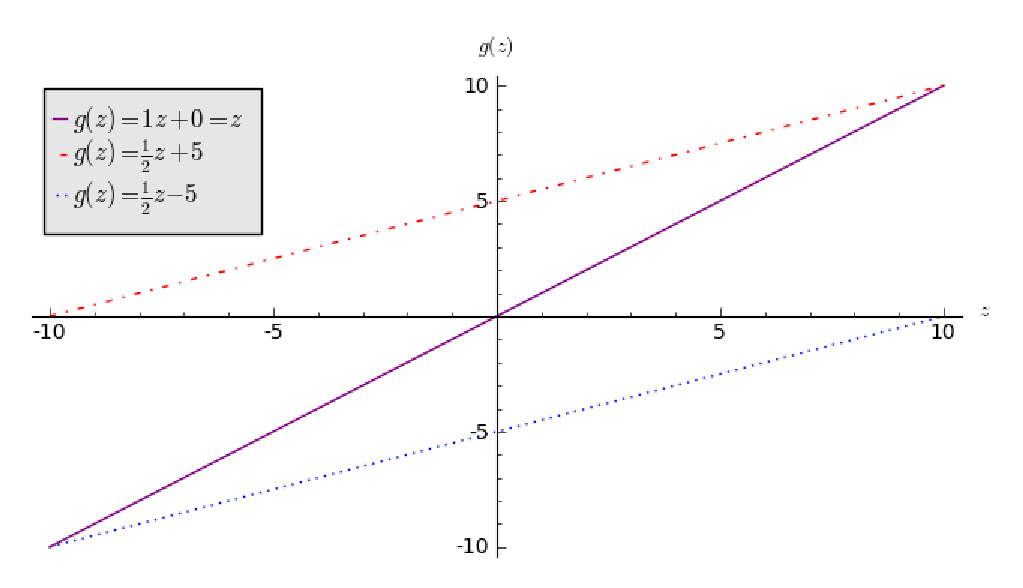
\includegraphics[width=8cm]{figures/LinearTransOfStdGaussianA.eps}}
\subfigure[{\scriptsize $g(z)=z$, $g(z)=(z+5)/0.5$ and $g(z)=(z-5)/0.5$.}]{
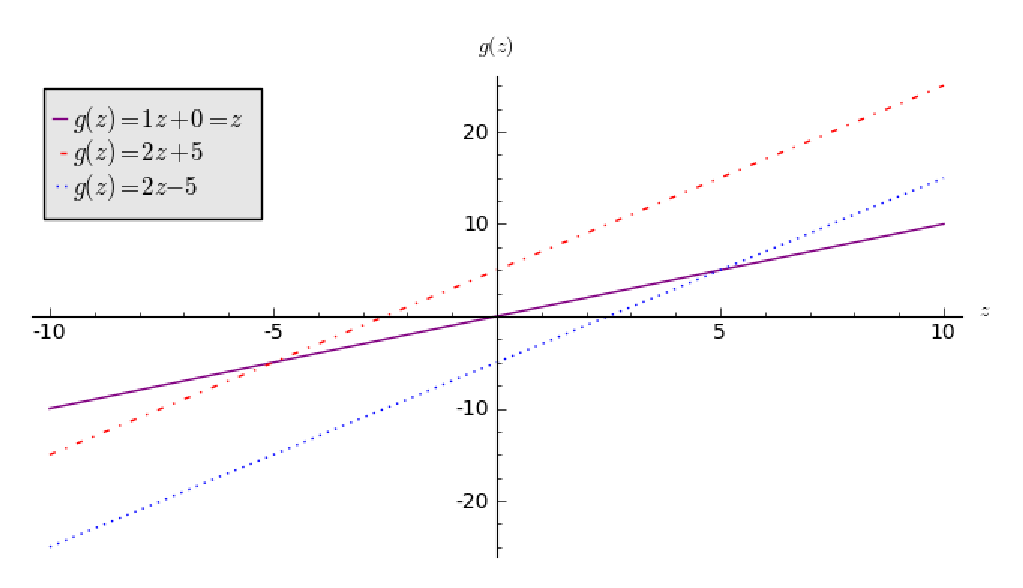
\includegraphics[width=8cm]{figures/LinearTransOfStdGaussianB.eps}}
\end{figure}

We are interested in the density of the tranformed random variable $Y=g(Z)=\sigma Z + \mu$.  
Once again, since $g$ is a one-to-one monotone function let us follow the four steps and use the change of variable formula to obtain $f_Y$ from $f_Z=\phi$ and $g$.
\begin{enumerate}
\item $y=g(z)=\sigma z + \mu$ is a monotone increasing function over $-\infty < z < \infty$, the range of $Z$.  
So, we can apply the change of variable formula. 
\item $z=g^{-1}(y)=(y - \mu) / \sigma$ is a monotone increasing function over the range of $y$ given by, %$(\sigma \times -\infty) + \mu < \sigma z + \mu < (\sigma \times \infty) + \mu$, i.e.,% Ben did not like these manipulaitons with infinities - raaz was doing arithmetic with diverging sequences with limits at infinity only. 
$-\infty < y < \infty$.  
\item For $-\infty < y < \infty$,
\[
 \left\vert \frac{d}{dy} g^{-1}(y) \right\vert 
= \left\vert \frac{d}{dy} \left( \frac{y - \mu}{\sigma} \right) \right\vert 
= \left\vert \frac{1}{\sigma} \right\vert = \frac{1}{\sigma} \enspace .
\]
\item we can use Equation~\eqref{E:f_YFromf_X_Under_one-to-one-g} and Equation~\eqref{E:StandardNormalPdf} which gives
$$f_Z(z) = \phi(z) = \frac{1}{\sqrt{2\pi}} \exp{\left( -\frac{z^2}{2}\right)} \enspace,$$
to find the density of $Y$ as follows:
\[
f_Y(y) = f_Z \left( g^{-1}(y) \right) \left\vert \frac{d}{dy} g^{-1}(y) \right\vert 
= \phi \left( \frac{y - \mu}{\sigma} \right) \frac{1}{\sigma}
= \frac{1}{\sigma \sqrt{2 \pi}} \exp \left[-\frac{1}{2} \left( \frac{y-\mu}{\sigma} \right)^2 \right] \enspace ,
\]
for $-\infty < y < \infty$. 
\end{enumerate}
Thus, we have obtained the expression for the probability density function of the linear transformation $\sigma Z + \mu$ of the standard normal random variable $Z$.  This analysis leads to the following definition.
\end{example}

%%%%%%%%%%%%%%%%%%%%%%%%%%%%%%%%%%%%%%%%%%%%%%%%%%%%%%%%%%%%%%%%
%%%%Location-scale Gaussian family as a linear transformation of the standard Gaussian RV

\begin{framed}

\begin{model}[$\normal(\mu,\sigma^2)$ RV]
Given a location parameter $\mu \in (-\infty, +\infty)$ and a scale parameter $\sigma^2 > 0$, the $\normal(\mu,\sigma^2)$ or Gaussian$(\mu,\sigma^2)$ random variable $X$ has probability density function:
\begin{equation}\label{eqn:norm_pdf}
f(x; \mu,
  \sigma^2)=\frac{1}{\sigma\sqrt{2\pi}}\exp\left[-\frac{1}{2}\left(\frac{x-\mu}{\sigma}\right)^2\right]\qquad(\sigma >0) \enspace .
\end{equation}
\end{model}
\end{framed}

This is simpler than it may at first look. $f(x;\mu, \sigma^2)$ has the following features.
\bit
\item $\mu$ is the expected value or mean parameter and $\sigma^2$ is the variance parameter. These concepts, mean and variance, are described in more detail in the next section on expectations.
\item $1/(\sigma\sqrt{2\pi})$ is a constant factor that makes the area under the curve of $f(x)$ from $-\infty$ to $\infty$ equal to 1, as it must be.
\item The curve of $f(x)$ is symmetric with respect to $x=\mu$ because the exponent is quadratic. Hence for $\mu=0$ it is symmetric with respect to the $y$-axis $x=0$.
\item The exponential function decays to zero very fast --- the faster the decay, the smaller the value of $\sigma$.
\eit

%\newpage

\begin{framed}
The normal distribution has the {\bf distribution function}
\begin{equation}\label{eqn:norm_int_cdf}F(x; \mu, \sigma^2)=\frac{1}{\sigma\sqrt{2\pi}}\int_{-\infty}^x\exp\left[-\frac{1}{2}\left(\frac{v-\mu}{\sigma}\right)^2\right]\;dv\enspace.\end{equation}
Here we need $x$ as the upper limit of integration and so we write $v$ in the integrand.
\end{framed}


\begin{figure}[ht]
\cen{
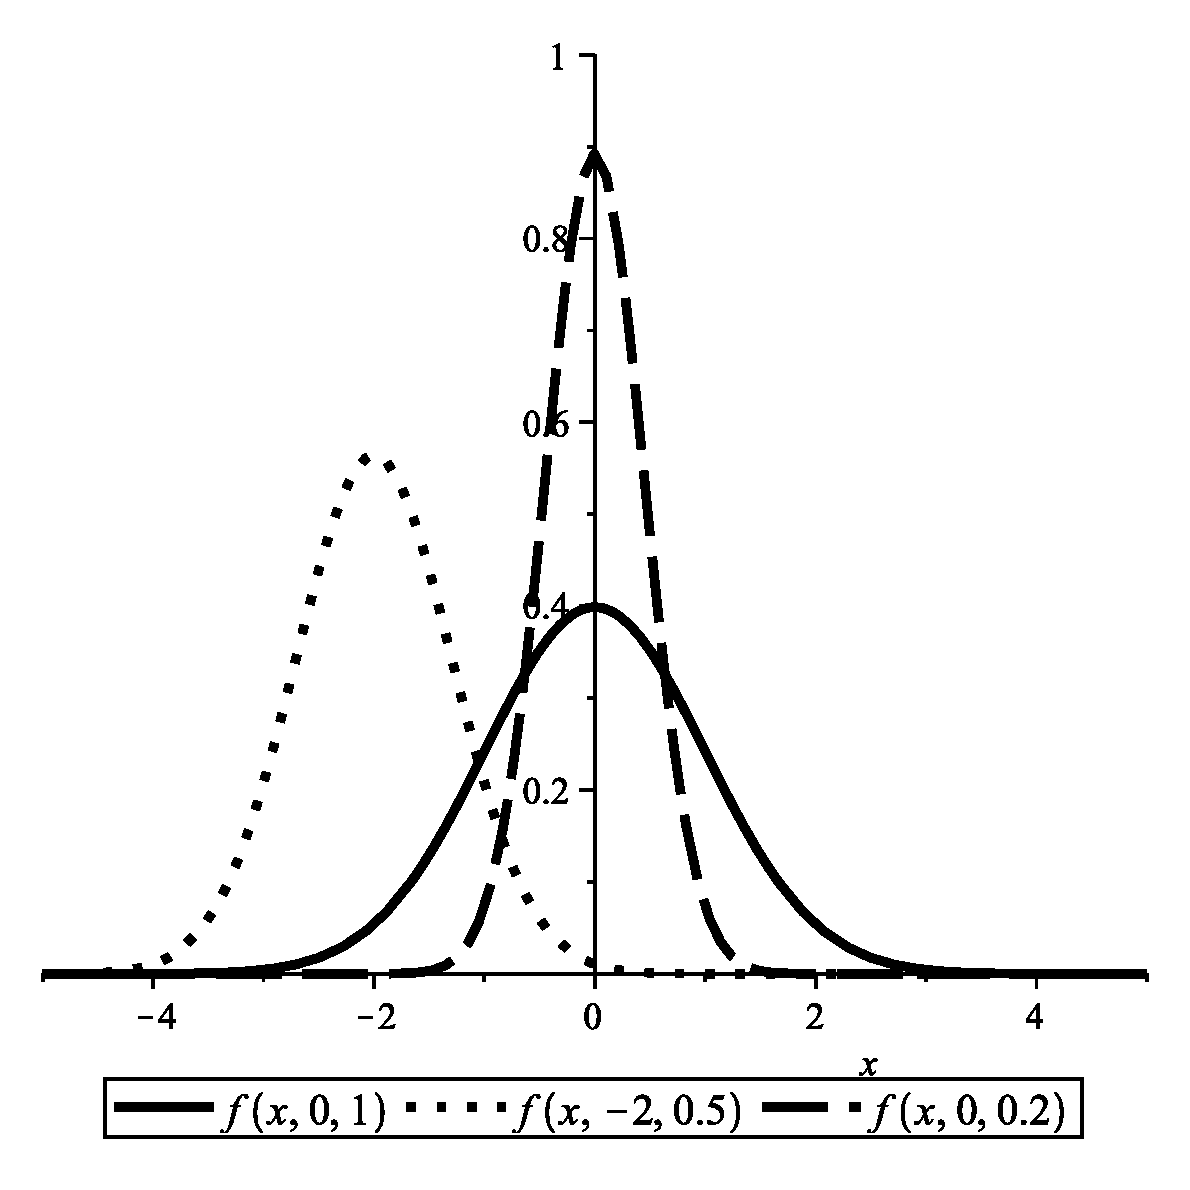
\includegraphics[scale=.3]{figures/normalpdf.eps}
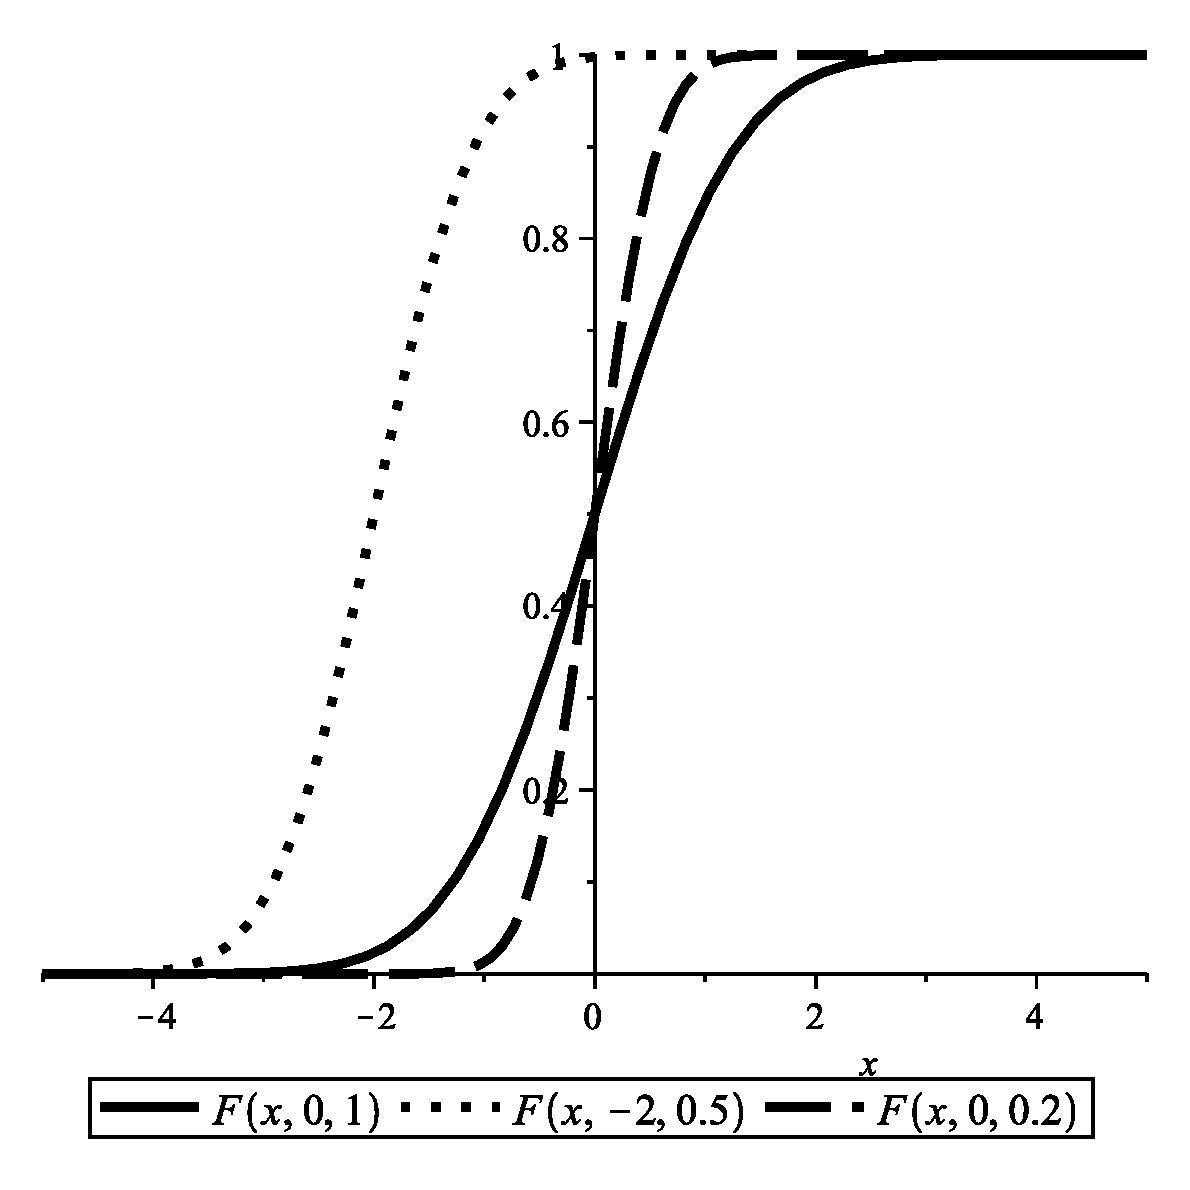
\includegraphics[scale=.3]{figures/normaldis.eps}
\caption{PDF and DF of a $\normal(\mu,\sigma^2)$ RV for different values of $\mu$ and $\sigma^2$}
}
\end{figure}

Using the direct method's \hyperref[Eqn:DirectMethod]{Equation~\ref*{Eqn:DirectMethod}}, we can obtain the distribution function of the $\normal(\mu,\sigma^2)$ random variable from that of the 
tabulated distribution function of the $\normal(0,1)$ in the  \hyperref[S:NormalDFTable]{Standard normal distribution function table in Sec.~\ref*{S:NormalDFTable}}. 
  
\begin{prop}[One Table to Rule Them All Gaussians]
The distribution function $F_X(x;\mu,\sigma^2)$ of the $\normal(\mu,\sigma^2)$ random variable $X$ 
and the distribution function $F_Z(z)=\Phi(z)$  of the standard normal random variable $Z$ are related by:
$$F_X(x;\mu,\sigma^2)\;=\; F_Z\left(\frac{x -\mu}{\sigma}\right) \;=\; \Phi\left(\frac{x-\mu}{\sigma}\right)\enspace .$$

\begin{proof}
Let $Z$ be a $\normal(0,1)$ random variable with distribution function $\Phi(z) = P (Z \leq z)$.  
We know that if $X=g(Z)=\sigma Z+\mu$ then $X$ is the $\normal(\mu,\sigma^2)$ random variable.  
Therefore, 
\begin{eqnarray*}
F_X(x;\mu,\sigma^2) 
&=& P(X \leq x) = P\left( g(Z) \leq x \right) =  P (\sigma Z+\mu \leq x) = P\left(Z \leq \frac{x -\mu}{\sigma} \right)\\ 
&=& F_Z \left(\frac{x -\mu}{\sigma}\right) = \Phi \left(\frac{x -\mu}{\sigma}\right) \enspace .
\end{eqnarray*}
\end{proof}
\end{prop}

Hence we often transform a general $\normal(\mu,\sigma^2)$ random
variable, $X$, to a standardised $\normal(0,1)$ random variable, $Z$, by
the substitution:
$$Z\;=\;\frac{X-\mu}{\sigma}\,.$$

\begin{example}\label{EgGaussianProbLocScaleFromTableMremsInFlight}
Suppose that the amount of cosmic radiation to which a person is exposed 
when flying by jet across the United States is a random
variable, $X$, having a normal distribution with a mean of $4.35$ mrem and a
standard deviation of $0.59$ mrem. What is the probability that a person
will be exposed to more than $5.20$ mrem of cosmic radiation on such a
flight?

{\em Solution:}
\begin{align*}
P(X> 5.20)\;&=\;1-P(X\leq
5.20)\\[3pt]&\;=\;1-F(5.20)\\[3pt]&\;=\;1-\Phi\left(\frac{5.20-4.35}{0.59}\right)\\[3pt]&\;=\;1-\Phi(1.44)\\[3pt]&\;=\;1-
0.9251\\[3pt]&\;=\;0.0749
\end{align*}
\end{example}

After some more notions you will see that $\normal(0,1)$ RV can actually be obtained from an IID process of $\bernoulli(\theta)$ RVs. This is an instance of the central limit theorem. To appreciate this we first need to understand what we mean by statistics and then familiarise ourselves with notions of convergence of random variables.


\subsubsection{Direct method}\label{S:DirectMethod}
If the transformation $g$ in $Y=g(X)$ is not necessarily one-to-one then special care is needed to obtain the distribution function or density of $Y$.  
For a continuous random variable $X$ with a known distribution function $F_X$ we can obtain the distribution function $F_Y$ of $Y=g(X)$ using Equation~\eqref{E:ProbOfgOfX} as follows:
\begin{eqnarray}\label{Eqn:DirectMethod}
F_Y(y)
&=& P \left(Y \leq y \right) = P \left(Y \in (-\infty, y] \right) \notag \\
&=& P \left( g(X) \in (-\infty, y] \right) = P \left( X \in g^{[-1]}((-\infty, y]) \right) = P \left(X \in \{x: g(x) \in (-\infty,y]\}  \right) \enspace . 
\end{eqnarray}
In words, the above equalities just mean that the probability that $Y \leq y$ is the probability that $X$ takes a value $x$ that satisfies $g(x) \leq y$.  
We can use this approach if it is reasonably easy to find the set $g^{[-1]}((-\infty,y]) = \{x: g(x) = (-\infty,y]\}$.% as done in Section~\ref{S:DirectMethod}.

\begin{example}\label{Exm:DirectMethodforYisXSquared}
Let $X$ be any random variable with distribution function $F_X$.  Let $Y=g(X)=X^2$.  
Then we can find $F_Y$, the distribution function of $Y$ from $F_X$ as follows:
\begin{itemize}
\item {Since $Y=X^2 \geq 0$, if $y < 0$ then $F_Y(y) = P\left( X \in \{ x : x^2 < y\} \right) = \p(X \in \emptyset) = 0$.}
\item {If $y \geq 0$ then
\begin{eqnarray*}
F_Y(y) = P \left(Y \leq y \right) 
&=& P \left( X^2 \leq y \right) \\
&=& P \left( -\sqrt{y} \leq X \leq \sqrt{y} \right) \\
&=& F_X(\sqrt{y}) - F_X(-\sqrt{y}) \enspace .
\end{eqnarray*}
}
\end{itemize}
By differentiation we get:
\begin{itemize}
\item {If $y<0$ then $f_Y(y)=\frac{d}{dy}(F_Y(y)) = \frac{d}{dy} 0 = 0$.}
\item {If $y \geq 0$ then
\begin{eqnarray*}
f_Y(y) 
= \frac{d}{dy}\left( F_Y(y) \right) 
&=& \frac{d}{dy}\left( F_X(\sqrt{y}) - F_X( - \sqrt{y}) \right)\\
&=& \frac{d}{dy}\left( F_X(\sqrt{y}) \right) - \frac{d}{dy}\left( F_X( - \sqrt{y}) \right)\\
&=& \frac{1}{2}y^{-\frac{1}{2}} f_X(\sqrt{y}) - \left( -\frac{1}{2}y^{-\frac{1}{2}} f_X( - \sqrt{y}) \right)\\
&=& \frac{1}{2 \sqrt{y}} \left( f_X(\sqrt{y}) + f_X( - \sqrt{y}) \right) \enspace .
\end{eqnarray*}
}
\end{itemize}
Therefore, the distribution function of $Y=X^2$ is:
\begin{equation}\label{E:F_YofX^2}
F_Y(y) = 
\begin{cases}
0 & \text{ if } y < 0 \\
F_X(\sqrt{y}) - F_X(-\sqrt{y}) & \text{ if } y \geq 0 \enspace .
\end{cases}
\end{equation}
and the probability density function of $Y=X^2$ is:
\begin{equation}\label{E:f_YofX^2}
f_Y(y) = 
\begin{cases}
0 & \text{ if } y < 0 \\
\frac{1}{2 \sqrt{y}} \left( f_X(\sqrt{y}) + f_X( - \sqrt{y}) \right) & \text{ if } y \geq 0 \enspace .
\end{cases}
\end{equation}
\end{example} 

\begin{example}\label{Eg:SquaredStdNormalIsChiSquared}
{If $X$ is the standard normal random variable with density 
$$f_X(x) = \phi(x) = \frac{1}{\sqrt{2 \pi}} \exp{(-x^2/2)}$$ 
then by Equation~\eqref{E:f_YofX^2} the density of $Y=X^2$ is:
\[
f_Y(y) = 
\begin{cases}
0 
& \text{ if } y < 0 \\
\frac{1}{2 \sqrt{y}} \left( f_X(\sqrt{y}) + f_X( - \sqrt{y}) \right)
=
\frac{1}{\sqrt{2 \pi y}} \exp\left(-\frac{y}{2}\right) 
& \text{ if } y \geq 0 \enspace .
\end{cases}
\]
$Y$ is called the {\bf chi-square} random variable with one degree of freedom. This distribution plays a fundamental role in hypothesis testing as we will see in Inference Theory and was derived at the beginning of last century to settle ``supposedly evidence-based disputes'' among scientists using mathematics.
}
\end{example}
\newpage

\section{Exercises in Transformations of Random Variables}\label{S:xsTransformationsOfRVs}
\begin{ExerciseList}
%transformation of RVs
\Exercise
Let $X$ be the outcome of a fair die roll with probability mass function given by
\[
f_X(x) = 
\begin{cases}
\frac{1}{6} & \text{ if } x \in \{1,2,3,4,5,6\}\\
0 & \text{ otherwise} \, .
\end{cases}
\]
If $Y = (X-3)^2$ then find the probability mass function of $Y$,  $f_Y (y)$.
\Answer
Using Equation~\eqref{E:PMFOfgOfX}, we can tabulate as follows:

\begin{tabular}{|c|c|c|c|c|}
\hline
$y$ & $0$ & $1$ & $4$ & $9$\\\hline
$f_Y(y)$ & $f_X(3)=\frac{1}{6}$ & $f_X(2)+f_X(4)=\frac{2}{6}$ & $f_X(1)+f_X(5)=\frac{2}{6}$ & $f_X(6)=\frac{1}{6}$\\\hline
\end{tabular}

\Exercise
Given a natural number $n$ as a parameter, i.e., given a parameter $n \in \{1,2,3,\ldots\}$, let $X$ be a discrete uniform random variable on the finite set
$$\mathbb{X}=\{-n,-n+1,\ldots,-1,0,1,\ldots,n-1,n\}$$
i.e.~the probability mass function of $X$ is:
\[
f_X(x;n) = 
\begin{cases}
\frac{1}{2n+1} & \text{ if } x \in \mathbb{X} \\
0 & \text{ otherwise}\, .
\end{cases}
\]
Find the probability mass function $f_Y(y;n)$ for $Y=|X|$, the absolute value of $X$.
\Answer
The probability mass function $f_Y(y;n)$ for $Y=|X|$, the absolute value of $X$, comes from applying the formula:
\[
f_Y(y;n) = \sum_{x \in \{ x: g(x)=y\}} f_X(x;n) \enspace ,
\]
as follows:
\[
f_Y(y) = 
\begin{cases}
\sum_{x \in \{ x: |x|=0\}} f_X(x;n) = f_X(0;n) = \frac{1}{2n+1} & \text{ if } y =0 \\
 \sum_{x \in \{ x: |x|=y\}} f_X(x;n) = \left( f_X(y;n)+f_X(-y;n) \right) = \frac{2}{2n+1} & \text{ if } y \in \{1,2,\ldots,n\} \\
0 & \text{otherwise}
\end{cases}
\]

\Exercise
If $X$ is a $\geometric(\theta)$ random variable and $Y=\left(\frac{1}{2}\right)^X$ then find an expression for $f_Y(y)$.
\Answer
We are given that $Y=2^{-X}$. Define the function
$$g: \{1,2,3,\ldots\} \to \{2^{-1},2^{-2},2^{-3},\ldots\}$$
by $y=g(x)=2^{-x}$.  Then $g$ is one-to-one and onto and so by Equation~\eqref{E:PMFOfgOfX},
\[
f_Y(y) = \sum_{x \in g^{[-1]}(y)} f_X(x) = \sum_{x \in g^{-1}(y)} f_X(x) = \sum_{x \in \{ -\log_2(y) \} } f_X(x) = f_X(-\log_2(y))\, .
\]
Note that the second equality above is emphasizing that the inverse image $g{[-1]}(y)$ is indeed the inverse function $g^{-1}(y)$ for this $g:\{1,2,3,\ldots\} \to \{2^{-1},2^{-2},2^{-3},\ldots\}$.  Therefore,
\[
f_Y(y) = 
\begin{cases}
f_X(-\log_2(y)) = \theta (1-\theta)^{-\log_2(y)-1} & \text{ if } y \in \{2^{-1},2^{-2},2^{-3},\ldots\}\\
0 & \text{ otherwise} \, .
\end{cases}
\]


\Exercise
If $X$ is a $\poisson(\lambda)$ random variable find the probability mass function,  $f_Y (y)$, of
\[
Y\,=\,\frac{1}{(X+1)^{2}} \enspace .
\]
\Answer
Since $X$ is a $\poisson(\lambda)$ random variable (by suppressing the `$;\lambda$' in the argument to $f_X(\cdot)$ for notational ease), we get
\[ f_X(x) \,=\, \P(X=x)\,=\, 
\begin{cases}
\frac{\lambda^x \, e^{-\lambda} }{ x!} & \text{ for }  x= 0, 1, 2, \dots \\
0 & \text{ otherwise} \,.
\end{cases}
\]

If $Y=(X+1)^{-2}=1/(X+1)^2$ then  \[ \{\ldots,2,1,0\} \ni x \xmapsto{(x+1)^{-2}} y \,\in\, \left\{1, \frac{1}{4}, \frac{1}{9}, \dots \right\} \]
and since $y=g(x)=(x+1)^{-2}$ {\scriptsize as it maps or associates each $y \in \left\{1, \frac{1}{4}, \frac{1}{9}, \dots \right\}$ to exactly one $x \in \{0,1,2,\ldots\}$ given by $g^{-1}(y)=y^{-1/2}-1 = \frac{1}{\sqrt{y}}-1= x$, its inverse function, this is because $g$ is {\em injective} or {\em one-to-one} as explained here if you want to recall quickly \url{https://en.wikipedia.org/wiki/Injective_function} again}, so we get:
\[
f_Y(y)\;=\; \P(Y=y)\;=\; \sum_{\{ x: g(x)=y\}}f_X(x)  \;=\; f_X\left( \frac{1}{\sqrt y}-1\right) \;=\; \frac{\lambda^{(\frac{1}{\sqrt y} -1)} \, e^{-\lambda}}{(\frac{1}{\sqrt y} -1)!}
\]
for $y = 1, \frac{1}{4}, \frac{1}{9}, \dots $, and $0$ otherwise.\\[4pt]
{\scriptsize CAUTION: This is a discrete RV and so don't just blindly apply the change of variable formula that only applies to continuous RV with a monotone and one-to-one function 
$g$ with inverse $g^{-1}$; it's just that in this discrete RV setting the inverse image also happens to satisfy these properties. But Poisson is discrete and `change of variable formula'' is hence inapplicable.}

\Exercise
If $X$ is a continuous random variable with probability density function
\[
f_X(x)\;=\;\begin{cases} x e^{- x} &  x\geqslant 0\\ 0 & x< 0\end{cases},
\]
find the probability density function of $Y\,=\, e^X$.
\Answer
Since  $y=g(x) = e^x$ is a monotone increasing function for $x \geqslant 0$,  we can apply the change of variable formula.

Now $x= g^{-1}(y) = \log_e(y)$ is a monotone increasing function for $y$ in $[1,\infty)$
\[\left|  \frac{d}{dy}\left(g^{-1}(y)\right)\right|\;=\; \left|  \frac{d}{dy}\left(\log_e(y)\right)\right|\;=\; \frac{1}{y}\,.\]

Therefore
\[
  f_Y(y) \;=\; f_X\left( \log_e(y)\right) \times  \left| \frac{1}{y} \right|\;=\;  \log_e(y) \,e^{-\log_e(y)} \times  \frac{1}{y} \;=\; \log_e(y) \, \frac{1}{y^2}
\]
since $e^{-\log_e(y)} = e^{\log_e(y^{-1})}  = y^{-1}$.

So the  probability density
  function  of $Y$ is given by
\[f_Y(y)\;=\;\begin{cases} \displaystyle  \frac{\log_e(y)}{y^2} &   \text{ if } x \geqslant 1 \\ 0 &
  \text{otherwise}
\end{cases} \,.
\]

\Exercise
If $X$, the received power at an antenna is an $\exponential(\lambda)$ random variable then find the probability density function of the amplitude $Y\,=\, \sqrt X$.
\Answer
Since $y=g(x) = \sqrt{x}$ is a monotone increasing function for $x \geqslant 0$,  we can apply the change of variable formula.

Now $x= g^{-1}(y) = y^2$ is a monotone increasing function for $y\geqslant 0$ so on this interval
\[
\left|  \frac{d}{dy}\left(g^{-1}(y)\right)\right|\;=\; \left|  \frac{d}{dy}\left( y^2\right)\right|\;=\; 2y\,.\]
Therefore
\[
f_Y(y) 
\;=\; f_X\left(  y^2\right) \times  \left| 2y \right|
\;=\;  \lambda e ^{-\lambda y^2} \times  2y  \;=\;   2 \lambda y e ^{-\lambda y^2}\,.
\]
So the  probability density function  of $Y$ is given by
\[
f_Y(y)\;=\;\begin{cases} \displaystyle  2 \lambda y e ^{-\lambda y^2}   &    y\geqslant 0 \\ 0 & y <0
\end{cases} \,.
\]


\Exercise
If $X$ is a $\uniform(a,b)$ random variable where $0 < a < b$, find  the probability density function, $f_Y (y)$, of \[ Y\,=\, \log_e(X) \, .\]
\Answer
First note that $y=g(x) = \log_e(x)$ is a monotone increasing function over  $a \leqslant x \leqslant b$, so we can apply the change of variable formula.

 $x= g^{-1}(y) = e^y$ is a monotone increasing function over $\log_e(a) \leqslant   \log_e(x) \leqslant \log_e(b)$, that is, over $\log_e(a) \leqslant   y \leqslant   \log_e(b)$.

For $\log_e(a) \leqslant   y \leqslant   \log_e(b)$,

\[\left|  \frac{d}{dy}\left(g^{-1}(y)\right)\right|\;=\; \left|  \frac{d}{dy}\left(e^y)\right)\right|\;=\; e^y\,.\]

Therefore 
\[
  f_Y(y) \;=\; f_X\left(g^{-1}(y)\right) \times  \left|  \frac{d}{dy} \left(g^{-1}(y)\right)\right|\;=\; \frac{1}{b-a} \times e^y\,.
\]
So the  probability density
  function  of $Y$ is given by  
\[f_Y(y)\;=\;\begin{cases} \displaystyle  \frac{e^y}{b-a}  &   \log_e(a)\leqslant x \leqslant \log_e(b)\\ 0 &
  \text{otherwise}
\end{cases} \,.
\]


\end{ExerciseList}



\section{Expectations}\label{S:Expectations}

Expectation is perhaps the most fundamental concept in probability theory. In fact, probability is itself an expectation as you will soon see!

Expectation is one of the fundamental concepts in probability.  The
expected value of a real-valued random variable gives the population mean, a measure of the
centre of the distribution of the variable in some sense.  
Its variance measures its spread and so on.

\begin{definition}[Expectation of a RV]
The {\bf expectation}, or {\bf expected value}, or {\bf mean}, or {\bf first moment}, of a random variable $X$, with distribution function $F$ and density $f$, is defined to be
\begin{equation}\label{E:Mean}
\e(X) := \int x\,dF(x) = 
\begin{cases}
\sum_x x f(x) & \qquad \text{if $X$ is discrete} \\
\int x f(x)\,dx  & \qquad \text{if $X$ is continuous} \  ,
\end{cases}
\end{equation}
provided the sum or integral is well-defined.  We say the expectation exists if
\begin{equation}\label{E:ExpectationExists}
\int \left|x\right|\,dF(x) < \infty \ .
\end{equation}
Sometimes, we denote $\e(X)$ by $\e X$ for brevity.  Thus, the expectation is a single-number summary of the RV $X$ and may be thought of  as the average.
We subscript $E$ to specify the parameter $\theta \in \BB{\Theta}$ with respect to which the integration is undertaken. 
\[
\e_{\theta} X := \int x\,dF(x;\theta)
\]
\end{definition}

\begin{definition}[Variance of a RV]\label{D:VarianceofX}
Let $X$ be a RV with mean or expectation $\e(X)$.  Variance of $X$ denoted by $\V(X)$ or $VX$ is
\[
\V(X) := \e \left((X-\e(X))^2\right) = \int (x-\e(X))^2 \,d F(x) \ ,
\]
provided this expectation exists.  The {\bf standard deviation} denoted by $\sd(X) := \sqrt{\V(X)}$.
Thus variance is a measure of ``spread'' of a distribution.
\end{definition}

\begin{definition}[$k$-th moment of a RV]
We call 
\[
\e(X^k) = \int x^k\,dF(x)
\]
as the $k$-th moment of the RV $X$ and say that the $k$-th moment exists when $\e(|X|^k) < \infty$.  We call the following expectation as the $k$-th central moment:
\[
\e \left((X- \e(X))^k\right) \ .
\]
\end{definition}

%%%%%%%%%%%%%%%%%%%%%%%%% fromPrsStEng

\subsection{Expectations of functions of random variables}\label{S:ExpectationsOfFunsOfRVs}

More generally, by taking the expected value of various functions of a random variable, we can measure many interesting features of its distribution, including spread and correlation.

\begin{definition}[Expectation of a function of a RV]\label{Df:expectation}
The \textbf{Expectation} of a function $g(X)$ of a random variable $X$ is defined as:
\[
\e(g(X))\; :=\; \int g(x) dF(x) = 
\begin{cases}
\displaystyle \sum_x g(x) f(x) & \text{if $X$ is a discrete RV}\\[12pt]
\displaystyle \int_{-\infty}^{\infty} g(x) f(x) dx & \text{if $X$ is a continuous RV}
\end{cases}
\]
provided $\e(g(X))$ exists, i.e., $\int |g(x)| dF(x) < \infty$.
\end{definition}

The {\bf mean} which characterises the central location of the random variable $X$ is merely the expectation of the identity function $g(x)=x$:
\[
\e(X)\; =\;
\begin{cases}
\displaystyle \sum_x x f(x) & \text{if $X$ is a discrete RV}\\[12pt]
\displaystyle\int_{-\infty}^{\infty} x f(x) dx & \text{if $X$ is a
  continuous RV}
\end{cases}
\]
Often, mean is denoted by $\mu$.

The \textbf{variance} which characterises the spread or the
  variability of the random variable $X$ is also the expectation of the
  function $g(x)=(x-\e(X))^2$:
\[
\V(X)\; =\; \e \left( (X-\e(X))^2 \right)\; =\;
\begin{cases}
\displaystyle\sum_x (x-\e(X))^2 f(x) & \text{if $X$ is a discrete RV}\\[12pt]
\displaystyle\int_{-\infty}^{\infty} (x-\e(X))^2 f(x) dx & \text{if $X$ is a continuous RV}
\end{cases}
\] 
Often, variance is denoted by $\sigma^2$. 

%\begin{framed}
INTUITIVELY, WHAT IS EXPECTATION?\\

Definition \ref{Df:expectation} gives expectation as a ``weighted average'' of the possible values. This is true but some intuitive idea of expectation is also helpful.
\begin{itemize}
\item Expectation is what you expect. \\[6pt]
Consider tossing a fair coin. If it is heads you lose \$10. If it is tails you win \$10. 
What do you expect to win? Nothing. 
If $X$ is the amount you win then $$\e(X)\;=\;-10\times \frac{1}{2}+10\times \frac{1}{2}\;=\;0\,.$$

So what you expect (nothing) and the weighted average ($\e(X)=0$) agree.


\item Expectation is a long run average.\\[6pt]
Suppose you are able to repeat an experiment independently, over and over again. 
Each experiment produces one value $x$ of a random variable $X$.  
If you take the average of the $x$ values for a large number of trials, then this average converges to $\e(X)$ as the number of trials grows.  In fact, this is called the {\bf law of large numbers}.
\end{itemize}
%\end{framed}

We can concretize the above two intuitive insights by the following two examples.

\begin{example}[Winnings on Average]\label{EgWinningsOnAverage}
Let $Y = r(X)$.  Then
\[
\e(Y) = \e(r(X)) = \int r(x)\, d F(x) \ .
\]
Think of playing a game where we draw $x \sim X$ and then I pay you $y=r(x)$.  Then your average income is $r(x)$ times the chance that $X=x$, summed (or integrated) over all values of $x$.
\end{example}

\begin{example}[Probability is an Expectation]\label{EgProbIsAnExpectation}
Let $A$ be an event and let $r(X)=\BB{1}_{A}(x)$.  Recall $\BB{1}_A(x)$ is $1$ if $x \in A$ and $\BB{1}_A(x)=0$ if $x \notin A$.  Then
\begin{equation}\label{E:ExpectationofIndicator}
\e(\BB{1}_A(X)) = \int \BB{1}_A(x)\, dF(x) = \int_A dF(x) = \p(X \in A) = \p(A)
\end{equation}
Thus, probability is a special case of expectation.  Recall our LTRF motivation for the definition of probability and make the connection.
\end{example}

\subsection*{Expectations of functions of $\Rz^2$-valued random variables}\label{S:ExpectationsOfFunsOf2RVs}

In the case of a single random variable we saw that its expectation gives the population mean, 
a measure of the center of the distribution of the variable in some sense.  
Similarly, by taking the expected value of various functions of a $\Rz^2$-valued random variable, we can measure many interesting features of its joint distribution.

\begin{definition}\label{Df:2expectation}
The \textbf{Expectation} of a function $g(X,Y)$ of the $\Rz^2$-valued RV $(X,Y)$ is defined as:
\[
\e(g(X,Y))\; =\;
\begin{cases}
\displaystyle \sum_{(x,y)} g(x,y) f_{X,Y}(x,y) & \text{if $(X,Y)$ is a discrete \rv}\\[12pt]
\displaystyle \int_{-\infty}^{\infty} \int_{-\infty}^{\infty} g(x,y) f_{X,Y}(x,y) dx dy & \text{if $(X,Y)$ is a continuous \rv}
\end{cases}
\]
\end{definition}

Some typical expectations for $\Rz^2$-valued random variables are:

\be
\item Joint Moments
\[
\e(X^r Y^s)
\]
When $r=s=1$, we have $\e(XY)$, the expectation of the product of two RVs.
\item 
We need a new notion for the variance of two RVs.

If $\e(X^2) < \infty$ and $\e(Y^2) < \infty$ then $\e(|X Y|) < \infty$ and $\e(|(X-\e(X))(Y-\e(Y))|) < \infty$.  This allows the definition of {\bf covariance} of $X$ and $Y$ as
\[
\cv(X,Y) := \e \left((X-\e(X))(Y-\e(Y))\right) = \e(X Y) - \e(X) \e(Y)
\]
\ee

The same ideas naturally extend, via multiple sums and integrals, to define the expectation of functions of $\Rz^k$-valued random variables with $k>2$.


\subsection*{Viewing a deterministic real variable as a random variable}

Consider the class of discrete RVs with distributions that place all probability mass on a single real number.  
This is the probability model for the deterministic real variable, which is often thought of as an unknown constant $\theta \in \Rz$.
\begin{model}[$\pointmass(\theta)$]
Given a specific point $\theta \in \Rz$, we say an RV $X$ has point mass at $\theta$ or is $\pointmass(\theta)$ distributed if the DF is:
\begin{equation}\label{E:PointMasscdf}
F(x;\theta) =
\begin{cases}
0 & \text{if $x < \theta$} \\
1 & \text{if $x \geq \theta$}
\end{cases}
\end{equation}
and the PMF is:
\begin{equation}
f(x;\theta) =
\begin{cases}
0 & \text{if  $x \neq \theta$} \\
1 & \text{if $x = \theta$}
\end{cases}
\end{equation}
\end{model}
Thus, $\pointmass(\theta)$ RV $X$ is deterministic in the sense that every realisation of $X$ is exactly equal to $\theta \in \Rz$.  We will see that this distribution plays a central limiting role in asymptotic statistics.

\begin{example}[Mean and variance of $\pointmass(\theta)$ RV]
Let $X \sim \pointmass(\theta)$.  Then:
\[
\e(X) = \sum_{x} x f(x) = \theta \times 1 = \theta \ , \qquad
\V(X) = \e(X^2) - (\e(X))^2 = \theta^2 - \theta^2 = 0 \ .
\]
\end{example}

\subsection{Properties of expectations}\label{S:PropOfEs}
The following results, where $a$ is a  constant, may easily be
proved using the properties of summations and integrals:

\bit
\item[] $\boxed{\e(a ) \,=\, a}$

\item[] $\boxed{\e(a \,g(X)) \,=\, a\, \e(g(X))}$

\item[] $\boxed{\e(g(X)+h(X))  \,=\, \e(g(X)) \,+\, \e(h(X))}$
\eit
Note that here  $g(X)$ and $h(X)$ are functions of the random variable
$X$: e.g.  $g(X)=X^2$.

Using these results we can obtain the following useful formula for variance:
\begin{eqnarray*}
V(X)
&=& E\left((X-\e(X))^2\right)\\[3pt]
& =& E \left( X^2 - 2 X \e(X) + (\e(X))^2 \right) \\[3pt]
&=& E ( X^2) - E \left( 2 X \e(X) \right) + E \left( (\e(X))^2
\right)\\[3pt]
& =& E ( X^2) - 2 \e(X) E \left( X \right) + (\e(X))^2 \\[3pt]
&=& E ( X^2) - 2 (\e(X))^2 + (\e(X))^2\\[3pt]
&=& \e(X^2) - (\e(X))^2 \enspace .
\end{eqnarray*}
That is, \[
\boxed{
V(X) \;=\; \e(X^2) \,- \,(\e(X))^2
}.
\]

The above properties of expectations imply that for constants $a$ and $b$,
%V(aX+b) = a^2 V(X) \enspace .
\begin{equation}\label{E:VofAffineofRVs}
\boxed{
\V(aX+b) = a^2\V(X) \ . 
}
\end{equation}

More generally, for random variables $X_1,X_2,\ldots,X_n$ and constants $a_1,a_2,\ldots,a_n$
\begin{itemize}
\item
\begin{equation}\label{E:EofLinCombofRVs}
\e \left( \sum_{i=1}^n a_i X_i \right) = \sum_{i=1}^n a_i \e(X_i) \ .
\end{equation}
%E \left( \sum_{i=1}^n a_i X_i \right) = \sum_{i=1}^n a_i \e(X_i)}$
%\smallskip
\item
%$\boxed{V \left(  \sum_{i=1}^n a_i X_i \right) = \sum_{i=1}^n a_i^2 V(X_i)}$, provided $X_1,X_2,\ldots,X_n$ are independent
\begin{equation}\label{E:VofLinCombofRVs}
\V \left(  \sum_{i=1}^n a_i X_i \right) = \sum_{i=1}^n a_i^2 \V(X_i) , \text{ provided $X_1,X_2,\ldots,X_n$ are independent}\ .
\end{equation}
\item Let $X_1,X_2,\ldots,X_n$ be independent RVs, then
\begin{equation}\label{E:EofProdIndRVs}
\e \left(  \prod_{i=1}^n X_i \right) = \prod_{i=1}^{n} \e(X_i) , \text{ provided $X_1,X_2,\ldots,X_n$ are independent}\ .
\end{equation}
\end{itemize}

%\item If the $k$-th moment exists and if $j<k$ then the $j$-th moment exists.

%\item $\V(X) = \e(X^2) - (\e(X))^2$ \ . [prove by completing the square and applying \eqref{E:EofLinCombofRVs}]
%\item If $a$ and $b$ are constants then:
%\item If $X_1,X_2,\ldots,X_n$ are independent and $a_1,a_2,\ldots,a_n$ are constants, then:
%\end{enumerate}

\subsection{Expectation of Common Random Variables}

Let us compute the mean and variance of our familiar RVs.

\begin{example}[Mean and variance of $\bernoulli(\theta)$ RV]\label{EgMeanAndVarOfBernoulli}
Let $X \sim \bernoulli(\theta)$.  Then, 
\[
\e(X) = \sum_{x=0}^1 x f(x) = (0 \times (1-\theta)) + (1 \times \theta) = 0+\theta=\theta \ ,
\]
\[
\e(X^2) =  \sum_{x=0}^1 x^2 f(x) =  (0^2 \times (1-\theta) ) + (1^2 \times \theta) = 0+\theta= \theta \ ,
\]
\[
\V(X) = \e(X^2) - (\e(X))^2 = \theta - \theta^2 = \theta(1-\theta) \ .
\]
Parameter specifically,
\[
\e_{\theta}(X)=\theta \qquad \text{and} \qquad \V_{\theta}(X)=\theta(1-\theta) \ .
\]
\begin{figure}[htpb]
\caption{Mean ($\e_{\theta}(X)$), variance ($\V_{\theta}(X)$) and the rate of change of variance ($\frac{d}{d \theta} \V_{\theta}(X)$) of a $\bernoulli(\theta)$ RV $X$ as a function of the parameter $\theta$.\label{F:MeanVarBernoulli}}
\centering   \makebox{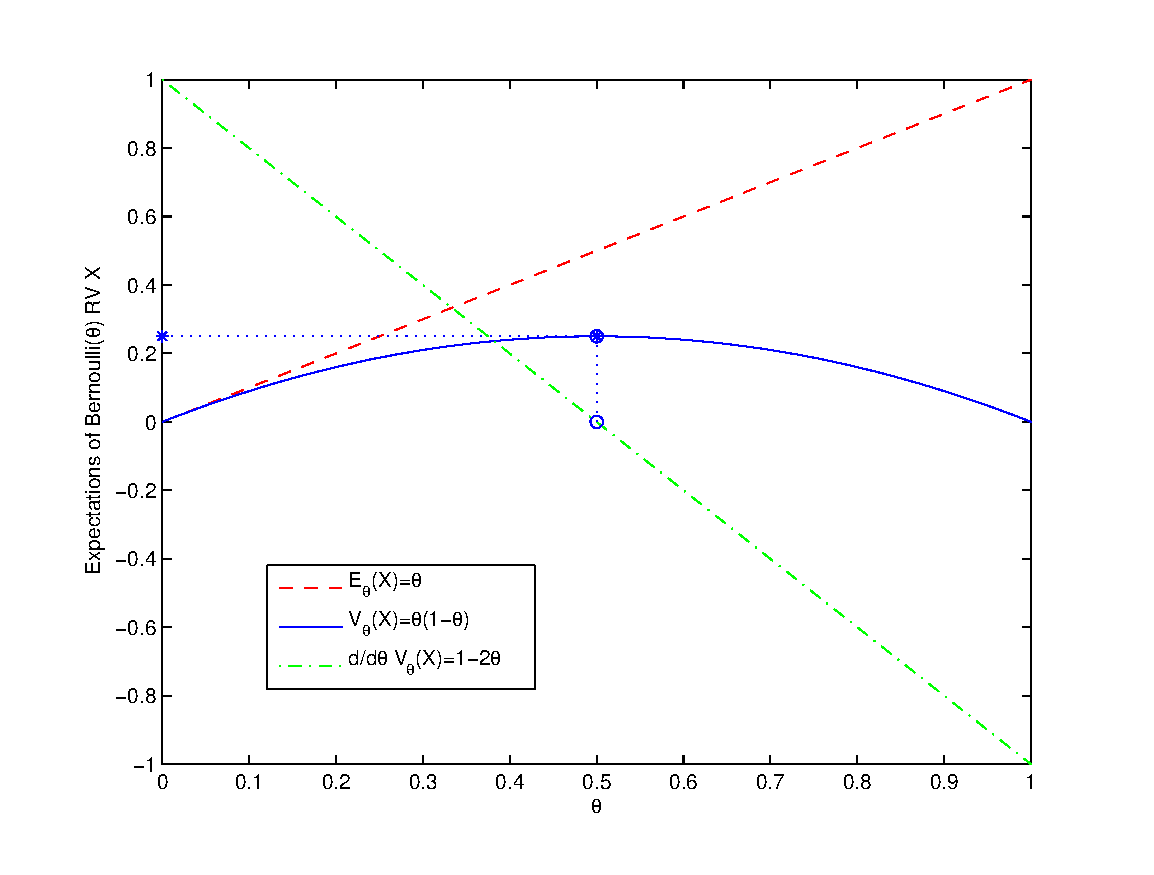
\includegraphics[width=5.0in]{figures/PlotMeanVarBernoulli}}
\end{figure}

Maximum of the variance $\V_{\theta}(X)$ is found by setting the derivative to zero, solving for $\theta$ and showing the second derivative is locally negative, i.e.~$\V_{\theta}(X)$ is concave down:
\[
\V_{\theta}'(X) := \frac{d}{d \theta} \V_{\theta}(X) = 1-2 \theta = 0  \iff \theta = \frac{1}{2} \ , 
\qquad \V_{\theta}''(X) := \frac{d}{d \theta} \left( \frac{d}{d \theta} \V_{\theta}(X) \right) = -2 < 0 \ ,
\]
\[
\max_{\theta \in [0,1]} \V_{\theta}(X) = \frac{1}{2} \left(1-\frac{1}{2} \right) = \frac{1}{4} \ , 
\text{since $\V_{\theta}(X)$ is maximized at $\theta = \frac{1}{2}$}
\]
The plot depicting these expectations as well as the rate of change of the variance are depicted in \hyperref[F:MeanVarBernoulli]{Figure \ref*{F:MeanVarBernoulli}}.  Note from this Figure that $\V_{\theta}(X)$ attains its maximum  value of $1/4$ at $\theta=0.5$ where $\frac{d}{d\theta}\V_{\theta}(X)=0$.  Furthermore, we know that we don't have a minimum at $\theta=0.5$ since the second derivative $\V_{\theta}''(X) = -2$ is negative for any $\theta \in [0,1]$.  This confirms that $\V_{\theta}(X)$ is concave down and therefore we have a maximum of $\V_{\theta}(X)$ at $\theta=0.5$.  We will revisit this example when we employ a numerical approach called Newton-Raphson method to solve for the maximum of a differentiable function by setting its derivative equal to zero.
\end{example}

\begin{example}[Mean and variance of $\uniform(0,1)$ RV]\label{EgMeanAndVarOfUnif01}
Let $X \sim \uniform(0,1)$.  Then, 
\[
\e(X) = \int_{x=0}^1 x f(x)\, dx = \int_{x=0}^1 x \ 1 \, dx = \frac{1}{2} \left( x^2 \right]_{x=0}^{x=1} = \frac{1}{2} \left( 1-0 \right) = \frac{1}{2} \ ,
\]
\[
\e(X^2) = \int_{x=0}^1 x^2 f(x)\, dx = \int_{x=0}^1 x^2 \ 1 \, dx =  \frac{1}{3} \left( x^3 \right]_{x=0}^{x=1} = \frac{1}{3} \left( 1-0 \right) = \frac{1}{3} \ ,
\]
\[
\V(X) = \e(X^2) - (\e(X))^2 = \frac{1}{3}  - \left( \frac{1}{2} \right)^2  = \frac{1}{3}  - \frac{1}{4} = \frac{1}{12} \ .
\]
\end{example}

\begin{Exercise}[title={Mean and variance of $\uniform(\theta_1,\theta_2)$ RV},label={xMeanAndVarOfUniformab}]
Let $X \sim \uniform(\theta_1,\theta_2)$ of Model~\ref{M:Uniformab}. Derive expressions for $\e(X)$ and $\V(X)$ in terms of the parameters $\theta_1$ and $\theta_2$. Make sure that when $\theta_2=1$ and $\theta_1=0$ you recover the expectation and variance of the $\uniform(0,1)$ RV in Example~\ref{EgMeanAndVarOfUnif01}.
\end{Exercise}
\begin{Answer}
Derive the answers from the definition of $\e(X)$ and $\V(X) = \e(X^2) - (\e(X))^2$ when $X \sim \uniform(\theta_1,\theta_2)$ with PDF given in Model~\ref{M:Uniformab}.
\[\e(X) = \frac{\theta_1+\theta_2}{2} \quad \V(\X) = \frac{(\theta_2-\theta_1)^2}{12}\]
\end{Answer}

\begin{example}[Expected Exponential of the $\uniform(0,1)$ RV]\label{EgExpectedExponentialOfUniform01}
Let $X \sim \uniform(0,1)$ and $Y=r(X)=e^X$.  Compute $\e(Y)$. 

We can simply apply the definition of $\e(r(X))$, since $Y=r(X)$, is just a function of $X$, as follows: 
\[
\e(Y) = \int_0^1 e^x f(x) dx = \int_0^1 e^x 1 \ dx = e-1 \ .
\]
%You could have also found out that the density $f(y)=1/y$ for the RV $Y$, provided $1<y<e$, and $0$ otherwise.  Again,
%\[
%\e(Y) = \int_1^e y f(y) dy = \int_1^e y \frac{1}{y} dy = \int_1^e 1 \ dy = e-1 \ .
%\]
\end{example}

\begin{example}[Mean and variance of $\exponential(\lambda)$]\label{EgmeanAndVarOfExponential}
Show that the mean of an $\exponential(\lambda)$ RV $X$ is:
\[
\e_{\lambda}(X) = \int_{0}^{\infty} x f(x;\lambda)\,dx
=   \int_{0}^{\infty} x \lambda e^{-\lambda x}\,dx
= \frac{1}{\lambda} \ ,
\]
and the variance is:
\[
\V_{\lambda}(X) = \left(  \frac{1}{\lambda} \right)^2 \ .
\]
\end{example}

\begin{example}[Mean and variance of $\geometric(\theta)$ RV]\label{EgmeanAndVarOfGeometric}
Let $X \sim \geometric(\theta)$ RV.  Then,
\[
\e(X) = \sum_{x=0}^{\infty} x \theta(1-\theta)^x =  \theta \sum_{x=0}^{\infty} x (1-\theta)^x
\]
In order to simplify the RHS above, let us employ differentiation with respect to $\theta$:
\[
\frac{-1}{\theta^2}= \frac{d}{d\theta} \left( \frac{1}{\theta} \right)= \frac{d}{d\theta} \sum_{x=0}^{\infty} (1-\theta)^x  =  \sum_{x=0}^{\infty} -x (1-\theta)^{x-1}
\]
Multiplying the LHS and RHS above by $-(1-\theta)$ and substituting in $\e(X)=  \theta \sum_{x=0}^{\infty} x (1-\theta)^x$, we get a much simpler expression for $\e(X)$ :
\[
\frac{1-\theta}{\theta^2}= \sum_{x=0}^{\infty} x (1-\theta)^{x} \implies \e(X) = \theta \left( \frac{1-\theta}{\theta^2} \right) = \frac{1-\theta}{\theta} \ .
\]
Similarly, it can be shown that
\[
\V(X) = \frac{1-\theta}{\theta^2} \ .
\]

\begin{figure}[htpb]
\caption{Mean and variance of a $\geometric(\theta)$ RV $X$ as a function of the parameter $\theta$.\label{F:MeanVarGeom}}
\centering   \makebox{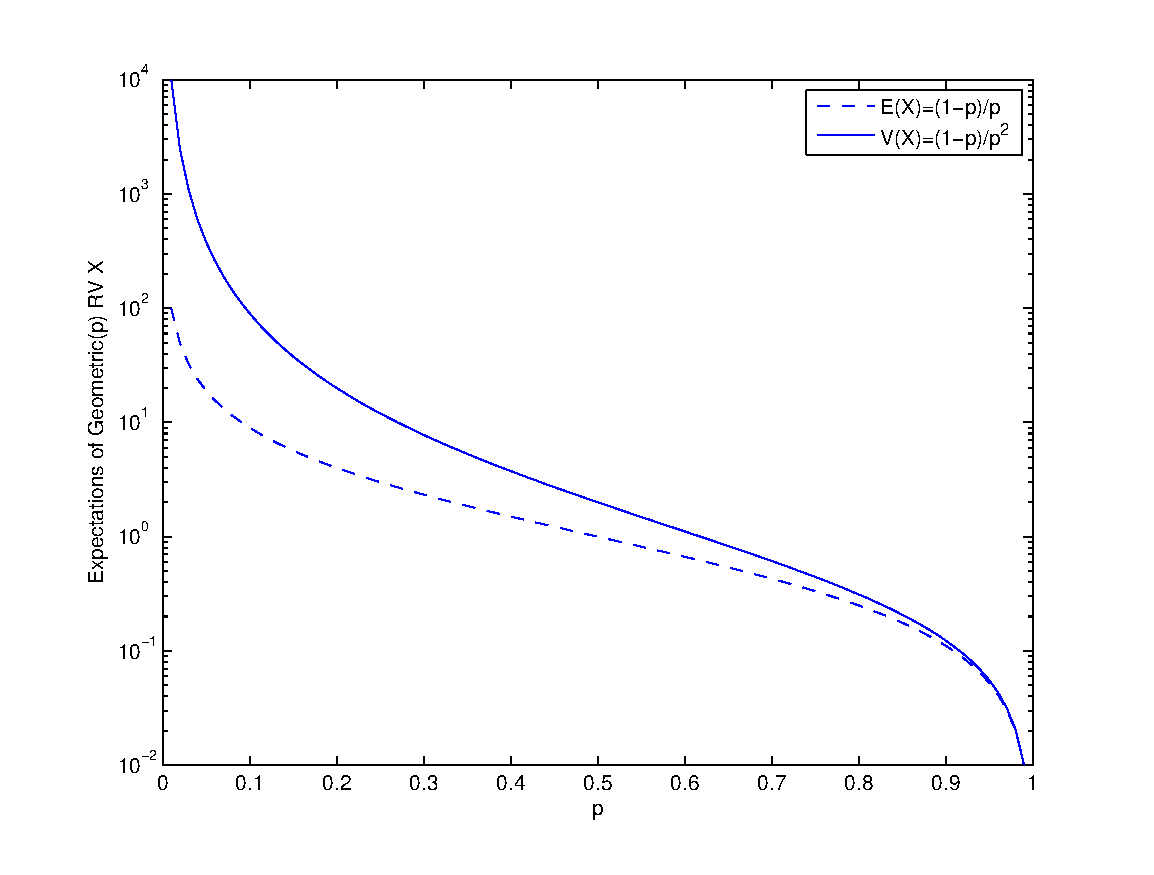
\includegraphics[width=5.0in]{figures/PlotMeanVarGeom}}
\end{figure}
\end{example}

% binomial model above
\begin{example}[Mean and variance of $\binomial(n,\theta)$ RV]\label{EgMeanAndVarOfBinomial}
Let $X \sim \binomial(n,\theta)$.  Based on the definition of expectation:
\[
\e(X) = \int x \, dF(x; n,\theta) = \sum_x x f(x;n,\theta) = \sum_{x =0}^n x \binom{n}{x} \theta^x (1-\theta)^{n-x} \ .
\]
However, this is a nontrivial sum to evaluate.  Instead, we may use \eqref{E:EofLinCombofRVs} and \eqref{E:VofLinCombofRVs} by noting that $X = \sum_{i=1}^n X_i$, where the $\{X_1,X_2,\ldots,X_n \} \overset{\IID}{\sim} \bernoulli(\theta)$, $\e(X_i) = \theta$ and $\V(X_i)=\theta(1-\theta)$:
\[
\e(X) = \e(X_1+X_2, \cdots ,X_n) = \e \left( \sum_{i=1}^n X_i \right) = \sum_{i=1}^n \e(X_i) = n \theta \ ,
\]
\[
\V(X) = \V \left( \sum_{i=1}^n X_i \right) = \sum_{i=1}^n \V(X_i) = \sum_{i=1}^n{\theta(1-\theta)} = n\theta(1-\theta) \ .
\]
\end{example}

\begin{example}[Mean and variance of $\poisson(\lambda)$ RV]\label{EgMeanAndVarOfPoisson}
Let $X \sim \poisson(\lambda)$.  Then:
\[
\e(X) = \sum_{x=0}^{\infty} x f(x;\lambda)
= \sum_{x =0}^{\infty} x \frac{ e^{-\lambda} \lambda^x}{x!}
= e^{-\lambda} \sum_{x =0}^{\infty} x \frac{  \lambda^x}{x!}
= e^{-\lambda} \sum_{x -1 =0}^{\infty} \frac{ \lambda \lambda^{x-1}}{(x-1)!}
= e^{-\lambda} \lambda e^{\lambda}
= \lambda
\ .
\]
Similarly,
\[
\V(X) = \e(X^2)-(\e(X))^2 = \lambda + \lambda^2 - \lambda^2 = \lambda \ .
\]
since
\begin{align*}
\e(X^2)& = \sum_{x=0}^{\infty} x^2 \frac{e^{-\lambda} \lambda^x}{x!} = \lambda \, e^{-\lambda} \sum_{x=1}^{\infty} \frac{x \, \lambda^{x-1}}{(x-1)!}
= \lambda \, e^{-\lambda} \left( 1 + \frac{2 \lambda}{1} + \frac{3 \lambda^2}{2!} + \frac{4 \lambda^3}{3!} + ... \right)\\
&= \lambda \, e^{-\lambda} \left( \left( 1 + \frac{\lambda}{1} + \frac{\lambda^2}{2!} + \frac{\lambda^3}{3!} + ... \right) + \left[ \frac{\lambda}{1} + \frac{2 \lambda^2}{2!} + \frac{3 \lambda^3}{3!} + ... \right] \right)\\
&= \lambda \, e^{-\lambda} \left( \left( e^{\lambda} \right) + \lambda \left( 1 + \frac{2 \lambda}{2!} + \frac{3 \lambda^2}{3!} + ... \right) \right)
= \lambda \, e^{-\lambda} \left( e^{\lambda} + \lambda \left( 1 + \lambda + \frac{\lambda^2}{2!} + ... \right) \right)\\
&= \lambda \, e^{-\lambda} \left( e^{\lambda} + \lambda \left( e^{\lambda} \right) \right)
= \lambda \, e^{-\lambda} \left( e^{\lambda} + \lambda\, e^{\lambda}\right) = \lambda (1 + \lambda) = \lambda + \lambda^2
\end{align*}

Note that $\poisson(\lambda)$ distribution is one whose mean and variance are the same, namely $\lambda$.
\end{example}

%\remove{
\begin{figure}[htpb]
\caption{PDF of $X \sim \poisson(\lambda=10)$ and the relative frequency histogram based on 1000 samples from $X$ according to Simulation~\ref{SIM:Poisson}.\label{F:PlotPdfSim1000HistPoiss10}}
\centering   \makebox{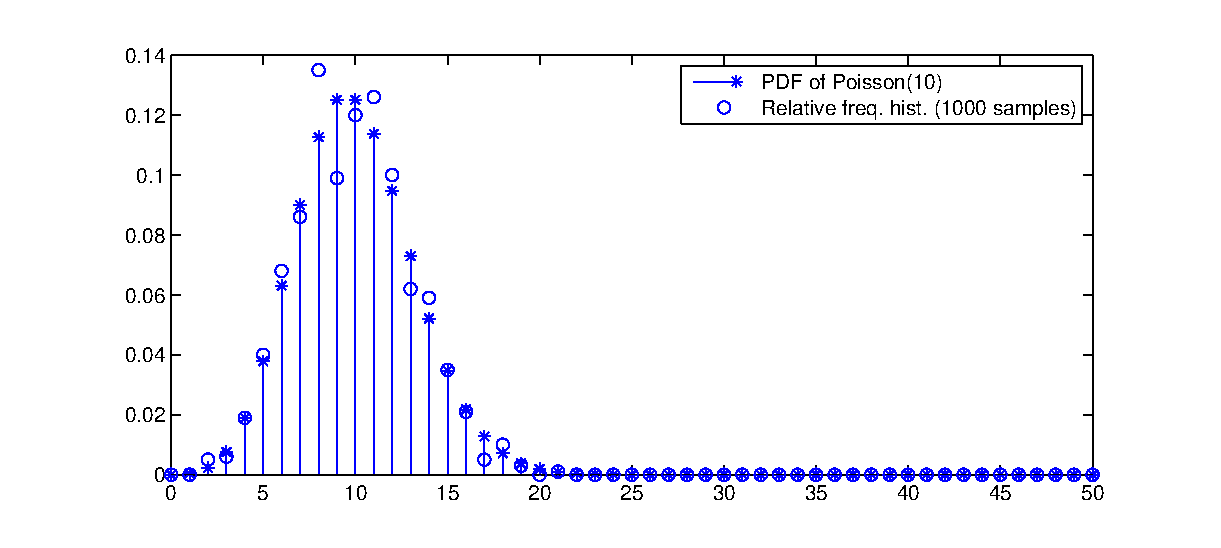
\includegraphics[width=6.50in]{figures/PlotPdfSim1000HistPoiss10}}
\end{figure}
%}%end remove

The $\poisson(\lambda)$ RV $X$ is also related to the IID $\exponential(\lambda)$ RV $Y_1,Y_2,\ldots$: $X$ is the number of occurrences, per unit time, of an instantaneous event whose inter-occurrence time is the IID $\exponential(\lambda)$ RV.  For example, the number of buses arriving at our bus-stop in the next minute, with exponentially distributed inter-arrival times, has a Poisson distribution.

\begin{example}[Mean and variance of $\normal(\mu,\sigma^2)$ RV]\label{EgMeanAndVarOfNormalMuSigmaSquareRV}
The location-scale family of RVs is indeed parameterised by its mean and variance, i.e., if  $X \sim \normal(\mu,\sigma^2)$ where $X=g(Z)= \sigma Z+\mu$ and $Z \sim \normal(0,1)$ then $\e(X) = \mu$ and $\V(X) = \sigma^2$ follows directly from the properties of Expectations, provided $\e(Z)=0$ and $\V(Z)=\e(Z^2)-\left(\e(Z)\right)^2=\e(Z^2)=1$.

The mean of a $\normal(0,1)$ RV $Z$ is:
\[
\e(Z) = \frac{1}{\sqrt{2 \pi}} \int_{-\infty}^{\infty} z \exp{\left( - \frac{1}{2} z^2 \right)}\,dz
 = \frac{1}{\sqrt{2 \pi}} \left(  -\exp{\left( - \frac{1}{2} z^2 \right)} \right]_{-\infty}^{\infty} 
= 0 \ ,
\]
and the variance is:
\[
\V(Z) =\e(Z^2)-\left(\e(Z)\right)^2=\e(Z^2)-0=\e(Z^2) = \frac{1}{\sqrt{2 \pi}} \int_{-\infty}^{\infty} z^2 e^{-z^2/2} dz .
\]
Using integration by parts with $u = z, dv=ze^{-z^2/2} \implies du=1, v=-e^{-z^2/2}, \, \int u dv = uv - \int v du$
\[
\frac{1}{\sqrt{2 \pi}} \int_{-\infty}^{\infty} z^2 e^{-z^2/2} dz =  \frac{1}{\sqrt{2 \pi}} \left( -z e^{-z^2/2} \right]_{-\infty}^{\infty} + \frac{1}{\sqrt{2 \pi}} \int_{-\infty}^{\infty} e^{-z^2/2} dz = 0 + 1 = 1
\]
The first term after the first equality above equals $0$ because the exponential goes to $0$ much faster than $z$ grows to $\pm \infty$. 
The second term equals $1$ because it is exactly the total probability integral of the PDF of the $\normal(0,1)$ RV.
\end{example}

Next, let us become familiar with an RV for which the expectation does not exist.  %This will help us appreciate the phrase ``none of which is dominant'' in the informal statement of the CLT later.
\begin{model}[$\cauchy$]\label{M:Cauchy}
The density of the $\cauchy$ RV $Y$ is:
\begin{equation}\label{E:StandardCauchypdf}
f(y) = \frac{1}{\pi (1+y^2)}, \qquad -\infty < y < \infty \enspace ,
\end{equation}
and its DF is:
\begin{equation}\label{E:StandardCauchycdf}
F(y) = \frac{1}{\pi} \tan^{-1} (y) + \frac{1}{2} \ .
\end{equation}
Randomly spinning a LASER emitting improvisation of ``Darth Maul's double edged lightsaber'' that is centered at $(1,0)$ in the plane $\Rz^2$ and recording its intersection with the $y$-axis, in terms of the $y$ coordinates of the point $(0,y)$, gives rise to the $Standard~Cauchy$ RV.

The Cauchy RV $Y$ can be derived from a RV $X \sim \uniform(-\pi/2,\pi/2)$ by the simple transformation $Y = \tan(X)$ for the above construction. 
Since $\tan(x)$ is one-to-one and monotone on the range of $X$ given by $(-\pi/2,\pi/2)$, 
we can use the change of variable formula in \hyperref[E:f_YFromf_X_Under_one-to-one-g]{Equation \ref*{E:f_YFromf_X_Under_one-to-one-g}} to obtain the PDF $f_Y(y)$ from the PDF $f_X(x)=\frac{1}{\pi}\BB{1}_{(-\pi/2,\pi/2)}(x)$ as follows:
\[
f_Y(y) = f_X(g^{-1}(y)) \left| \frac{d}{dy} g^{-1}(y) \right| = f_X(\tan^{-1}(y)) \left| \frac{d}{dy} \tan^{-1}(y) \right| = \frac{1}{\pi} \left| \frac{1}{1+y^2} \right|
\]
Note that the construction is valid even if we sample $X$ uniformly from $(0,\pi)$ and take its $\tan(X)$.
\end{model}

\begin{example}[Mean of $\cauchy$ RV]
The expectation of the $\cauchy$ RV $X$, obtained via integration by parts (set $u=x$ and $v=\tan^{-1}(x)$) does not exist  %\eqref{E:ExpectationExists}
, since:
\begin{equation}\label{E:CauchyMeanDoesNotExist}
\int \left|x\right|\,dF(x) = \frac{2}{\pi} \int_0^{\infty} \frac{x}{1+x^2}\,dx = \left(x \tan^{-1}(x) \right]_0^{\infty} - \int_0^{\infty} \tan^{-1}(x)\, dx = \infty \ .
\end{equation}
Note that we consider symmetry of integral about the origin and take twice the integral over $(0,\infty)$ above. 
Variance and higher moments cannot be defined when the expectation itself is undefined.
\end{example}

Next let us consider a natural generalization of the $\bernoulli(\theta)$ RV with more than two outcomes but in the set $\{1,2,\ldots,k\}$.
\begin{model}[{$\demoivre(\theta_1,\theta_2,\ldots,\theta_k)$}]\label{M:demoivre}
Given a specific point $(\theta_1,\theta_2,\ldots,\theta_k)$ in the unit $k-1$-Simplex:
\[
\bigtriangleup^{k-1} :=  \{ \,  ( \theta_1,\theta_2,\ldots,\theta_k) :  \theta_1 \geq 0, \theta_2 \geq 0, \ldots, \theta_k \geq 0, \sum_{i=1}^k \theta_i = 1 \, \}  \ ,
\]
we say that an RV $X$ is $\demoivre(\theta_1,\theta_2,\ldots,\theta_k)$ distributed if its PMF is:
\[
f(x;\theta_1,\theta_2,\ldots,\theta_k) =
\begin{cases}
0 & \quad \text{if $x \notin [k] := \{1,2,\ldots,k\}$,} \\
\theta_x & \quad \text{if $x \in [k]$}   .
\end{cases}
\]
The DF for $\demoivre(\theta_1,\theta_2,\ldots,\theta_k)$ RV $X$ is:
\begin{equation}\label{E:deMoivreDF}
F(x;\theta_1,\theta_2,\ldots,\theta_k) =
\begin{cases}
0 & \quad  \text{if $-\infty < x < 1$}\\
\theta_1 & \quad \text{if $1 \leq x < 2$} \\
\theta_1+\theta_2 & \quad \text{if $2 \leq x < 3$} \\
\vdots & \\
\theta_1+\theta_2+\cdots+\theta_{k-1} & \quad \text{if $k-1 \leq x < k$} \\
\theta_1+\theta_2+\cdots+\theta_{k-1}+\theta_k=1 & \quad \text{if $k \leq x < \infty$} \\
\end{cases}
\end{equation}
The $\demoivre(\theta_1,\theta_2,\ldots,\theta_k)$ RV can be thought of as a probability model for ``the outcome  of rolling a polygonal cylindrical die with $k$ rectangular faces that are marked with $1, 2, \ldots, k$''.  The parameters $\theta_1,\theta_2,\ldots,\theta_k$ specify how the die is loaded and may be idealised as specifying the cylinder's centre of mass with respect to the respective faces.  Thus, when $\theta_1=\theta_2=\cdots=\theta_k=1/k$, we have a probability model for the outcomes of a fair die.
\end{model}

\paragraph{Mean and variance of $\demoivre (\theta_1,\theta_2,\ldots,\theta_k)$ RV:}
The not too useful expressions for the first two moments of $X \sim \demoivre (\theta_1,\theta_2,\ldots,\theta_k)$ are,
\[
\e(X) = \sum_{x=1}^k x \theta(x) =  \theta_1 + 2 \theta_2 + \cdots + k \theta_k \ , \text{ and }
\]
\[
\V(X) = \e(X^2) - (\e(X))^2 =   \left(\theta_1 + 2^2 \theta_2 + \cdots + k^2 \theta_k \right) - \left( \theta_1 + 2 \theta_2 + \cdots + k \theta_k \right)^2 \ .
\]
However, if $X\sim \demoivre(1/k,1/k,\ldots,1/k)$, then the mean and variance for the fair $k$-faced die based on Faulhaber's formula for $\sum_{i=1}^k i^m$, with $m\in\{1,2\}$, are,
\[
\e(X) = \frac{1}{k} \left( 1+2+\cdots+k \right)= \frac{1}{k} \frac{k(k+1)}{2} = \frac{k+1}{2}  \ ,
\]
\[
\e(X^2) = \frac{1}{k} \left( 1^2+2^2+\cdots+k^2 \right)  = \frac{1}{k} \frac{k(k+1)(2k+1)}{6} =  \frac{2k^2+3k+1}{6} \ ,
\]
\begin{align}
\V(X) = \e(X^2) - (\e(X))^2
&= \frac{2k^2+3k+1}{6} -  \left( \frac{k+1}{2} \right)^2 = \frac{2k^2+3k+1}{6} -  \left( \frac{k^2+2k+1}{4} \right) \notag \\
&=  \frac{8k^2+12k+4 - 6k^2-12k-6}{24} =  \frac{2k^2-2}{24} = \frac{k^2-1}{12} \notag \ .
\end{align}


\section{Exercises in Expectations of Random Variables}\label{S:xsExpectationsOfRVs} %S:xsMultivariateRVs
\begin{ExerciseList}
\Exercise
Let $X$ be the number of air
  conditioners a  store  sells each day, and assume that $X$ has
  probability mass function $f(10)=0.1$, $f(11)=0.3$,
  $f(12)=0.4$, $f(13)=0.2$.
\be
\item  Find the expected number of conditioners that the store sells
  each day.
\item If the profit per conditioner is $\$55$, what is the expected daily profit?
\ee
\Answer
\be
\item
The expected number of conditioners that the store sells daily  is
\ba{\e(X)&=\;\sum_{i=1}^{n}x_ip_{x_i}\\[6pt]
&=(10\times0.1+11\times0.3+12\times0.4+13\times0.2)\\[6pt]
&=1+3.3+4.8+2.6\\[6pt]
&=11.7\enspace . }
\item
The profit per conditioner is $\$55$, and so the expected daily profit given by
\[E( 55 \,X)\;=\; 55 E(X) \;=\; 55 \times 11.7 \;=\; 643.50\, ,\]
is $\$643.50$.
\ee

\Exercise
A small petrol station is supplied with fuel  every Saturday
  afternoon. Assume that its volume of sales $X$, in ten thousands of
  litres, has density
$$f(x)\;=\;\begin{cases}6x(1-x)&0\leq x \leq
  1\\0&\textrm{otherwise}\end{cases}\,.$$
Determine the mean and  variance of $X$.
\Answer
The expected value $\e(X)$ is
\ba{\e(X)&=\int^1_0 6x(1-x)x\,dx\\
&=\;\int^1_0 (6x^2-6x^3)\,dx\\[3pt]
&=\;\left. 2x^3-\frac{6}{4}x^4\right]^1_0\\
&=\;2(1^3-0)-\frac{6}{4}(1^4-0)\\
&=\;0.5}

\ba{\e(X^2)&=\int^1_0 6x(1-x)x^2\,dx\\[3pt]
&=\;\int^1_0 6x^3-6x^4\,dx\\[3pt]
&=\;\left.\frac{6}{4}x^4-\frac{6}{5}x^5\right]^1_0\\
&=\;\frac{6}{4}(1^4-0)-\frac{6}{5}(1^5-0)\\
&=0.3  
}
the variance is $\V(X)\;=\;\e(X^2)-(\e(X))^2\;=\;0.3-0.5^2\;=\;0.05$

\Exercise
Starting from the definition of the variance of a random variable (Definition~\ref{D:VarianceofX}) show that
\[\V(X) = \e(X^2) - \left(\e(X)\right)^2 \enspace .\]
\Answer
This was already done in Sec.~\ref{S:PropOfEs} on Properties of Expectation. Make sure you understand each step.

\Exercise
Show that $V(aX+b) = a^2 V(X)$ for constants $a$ and $b$ and a random variable $X$.
\Answer
Using the definition of variance, expectations and by completing the square, we get:
\begin{multline*}
V(aX+b) = E ((aX+b)^2) - (E(aX+b))^2 = E \left( (aX)^2 + 2aXb + b^2 \right) - \left( aE(X)+b\right)^2 \\
= a^2 E \left(X^2\right) + 2ab E(X) + b^2 - a^2(E(X))^2 - 2abE(X) - b^2
= a^2 \left( E \left(X^2\right) - (E(X))^2 \right) = a^2 V(X) \, .
\end{multline*}

\Exercise
{**}Let $X$ be a discrete random variable with PMF given by
\[
f(x) = 
\begin{cases}
\frac{x}{10} & \text{ if } x \in \{1,2,3,4\} ,\\
0 & \text{ otherwise.}
\end{cases}
\]
\begin{itemize}
\item[(a)] Find:
\begin{itemize}
\item[(i)] $\p(X=0)$
\item[(ii)] $\p(2.5 < X < 5)$
\item[(iii)] $\e(X)$
\item[(iv)] $\V(X)$
\end{itemize}
\item[(b)] Write down the DF (or CDF) of $X$.
\item[(c)] Plot the PMF and CDF of $X$.
\end{itemize}

\Exercise
Find the mean and the variance of the following  random variables.
\be
\item $X$ a discrete uniform random variable on $\{1,2,3,4,5,6\}$, i.e., \textit{the number a fair die turns up}.
 \item $X$ is a $\uniform(0,8)$ random variable, i.e., \textit{a continuous uniform random variable from the interval} $[0,8]$.

\item $X$ has a density function
$$
f(x)\,=\, 
\begin{cases} 
2e^{-2x} & \text{ if }  x \geq 0\\ 
0 & \text{ otherwise} \, . 
\end{cases}
$$
\ee
\Answer
\be
\item
The probability mass function of $X$ is
$$f(x)=\begin{cases}\frac{1}{6}&x=1\\
\frac{1}{6}&x=2\\
\frac{1}{6}&x=3\\
\frac{1}{6}&x=4\\
\frac{1}{6}&x=5\\
\frac{1}{6}&x=6
\end{cases}$$
and so
$$\e(X)\;=\;\sum_{i=1}^6
x_if(x_i)\;=\;\frac{1}{6}+\frac{2}{6}+\frac{3}{6}+\frac{4}{6}+\frac{5}{6}+\frac{6}{6}\;=\;3.5\,.$$
Now,
$$\e(X^2)\;=\;\sum_{i=1}^6 x^2_if(x_i)\;=\;\frac{1}{6}+\frac{4}{6}+\frac{9}{6}+\frac{16}{6}+\frac{25}{6}+\frac{36}{6}\;=\;\frac{91}{6}\;=\;15.1667$$
and so  the variance is
\[V(X)\; =\; \e(X^2) - (\e(X))^2 \;=\; 15.1667-3.5^2\;=\;2.9167\,.\] 
  
\item The density function of the uniform distribution, $X$,  on $[0,8]$ is  $$f(x)=\begin{cases}\frac{1}{8}&0<x<8\\0&\textrm{otherwise}\end{cases}$$
Therefore, $$\e(X)\;=\;\frac{8+0}{2}\;=\;4\enspace,$$
and $$\V(X)\;=\;\frac{(8-0)^2}{12}\;=\;\frac{16}{3}$$

\item Since $f(x)$ is the density function of an $\exponential(\lambda)$ random variable with parameter $\lambda=2$, we can use earlier results to get
$$\e(X)\;=\;\frac{1}{2}\quad \text{and}\quad
\V(X)\;=\;\frac{1}{4}\enspace.$$

(You should also be able to do this by integration!)
\ee

\end{ExerciseList}



\section{Multivariate Random Variables}\label{S:RVecs}

Often, in experiments we are measuring two or more aspects simultaneously.  
For example, we may be measuring the diameters and lengths of cylindrical shafts manufactured in a plant or heights, weights and blood-sugar levels of individuals in a clinical trial.  
Thus, the underlying outcome $\omega \in \Omega$ needs to be mapped to measurements as realizations of random vectors in the real plane $\Rz^2 = (-\infty, \infty) \times (-\infty, \infty)$ or the real space $\Rz^3 = (-\infty, \infty) \times (-\infty, \infty) \times (-\infty, \infty)$:
\[
\omega \mapsto \left( X(\omega),Y(\omega) \right) : \Omega \to \Rz^2  \qquad \qquad \qquad \omega \mapsto \left( X(\omega),Y(\omega), Z(\omega) \right) : \Omega \to \Rz^3
\]
%\vspace{2cm}

More generally, we may be interested in heights, weights, blood-sugar levels, family medical history, known allergies, etc. of individuals in the clinical trial and thus need to make $m$ measurements of the outcome in $\Rz^m$ using a ``measurable mapping'' from $\Omega \to \Rz^m$.  
To deal with such multivariate measurements we need the notion of {\bf random vectors} ({\rv}s), i.e.~ordered pairs of random variables $(X,Y)$, ordered triples of random variables $(X,Y,Z)$, or more generally ordered $m$-tuples of random variables $(X_1,X_2,\ldots,X_m)$.  

\subsection{$\Rz^2$-valued Random Variables}

We first focus on understanding $(X,Y)$, a bivariate \rv~or $\Rz^2$-valued RV that is obtained from a pair of discrete or continuous RVs.  
We then generalize to $\Rz^m$-valued RVs with $m>2$ in the next section.

\begin{definition}[JDF]\label{Df:JDF}
The {\bf joint distribution function (JDF)} or {\bf joint cumulative distribution function (JCDF)}, $F_{X,Y}(x,y):\mathbb{R}^2\to [0,1]$, of the bivariate random vector $(X,Y)$ is
\begin{eqnarray}\label{E:j2DF}
F_{X,Y}(x,y)\; 
&=& \p(X\leq x \cap Y \leq y) \;= \;\p(X\leq x , Y \leq y)\notag\\
&=& P\left( \{ \omega: X(\omega) \le x, Y(\omega) \le y \} \right) \mbox{, for any } (x,y) \in \mathbb{R}^2 \enspace ,
\end{eqnarray}
where the right-hand side represents the probability that the random vector $(X,Y)$ takes on a value in 
$\{(x',y'): x' \leq x, y' \leq y\}$, the set of points in the plane that are south-west of the point $(x,y)$.
\end{definition}

The JDF $F_{X,Y}(x,y):\Rz^2\to\Rz$ satisfies the following conditions to remain a probability: 
\begin{enumerate}
\item $0 \leq F_{X,Y}(x,y) \leq 1$
\item $F_{X,Y}(x,y)$ is an non-decreasing function of both $x$ and $y$
\item $F_{X,Y}(x,y) \to 1$ as $x\to \infty$ and $y\to \infty$
\item $F_{X,Y}(x,y) \to 0$ as $x\to -\infty$ and $y\to -\infty$
\end{enumerate}

\begin{definition}[JPMF]
If $(X,Y)$ is a {\bf discrete random vector} that takes values in a discrete support set $\mathcal{S}_{X,Y} = \{(x_i,y_j): i=1,2,\ldots, \, j=1,2,\ldots\} \subset \Rz^2$ with probabilities $p_{i,j}=\p(X=x_i,Y=y_j)>0$, then its \textbf{joint probability mass function} (or JPMF) is:
\begin{equation}\label{Eq:j2DPMF}
f_{X,Y}(x_i,y_j) = \p(X=x_i,Y=y_j) %P\left(\{\omega: X(\omega) = x_i, Y(\omega)=y_j \}\right) 
=\begin{cases}
p_{i,j}&\quad \textrm{if } (x_i,y_j) \in \mathcal{S}_{X,Y}\\
0&\quad \textrm{otherwise}
\end{cases}  \enspace .
\end{equation}

Since $\p(\Omega)=1$, $\sum_{{\substack{(x_i,y_j) \in \mathcal{S}_{X,Y}}}}f_{X,Y}(x_i,y_j)=1$.
\end{definition}

From JPMF $f_{X,Y}$ we can get the values of the JDF $F_{X,Y}(x,y)$ and the probability of any event $B$ by simply taking sums,
\begin{equation}\label{Eq:2DiscretejDFFromjPMF}
\boxed{F_{X,Y}(x,y)\;=\;\sum_{x_i\leq x, y_j \leq y}f_{X,Y}(x_i,y_j) }\enspace ,
\qquad \boxed{\p(B)\;=\;\sum_{\substack{(x_i, y_j) \in B \cap \mathcal{S}_{X,Y}}}f_{X,Y}(x_i,y_j) }\enspace ,
\end{equation}

\begin{example}\label{Eg:Discrete2DPMF}
Let $(X,Y)$ be a discrete bivariate \rv with the following joint probability mass function (JPMF):
\[
f_{X,Y}(x,y) := P (X=x,Y=y)  = 
\begin{cases}
0.1 & \text{ if } (x,y)=(0,0)\\
0.3 & \text{ if } (x,y)=(0,1)\\
0.2 & \text{ if } (x,y)=(1,0)\\
0.4 & \text{ if } (x,y)=(1,1)\\
0.0 & \text{ otherwise.}
\end{cases} 
\]
\begin{center}
\makebox{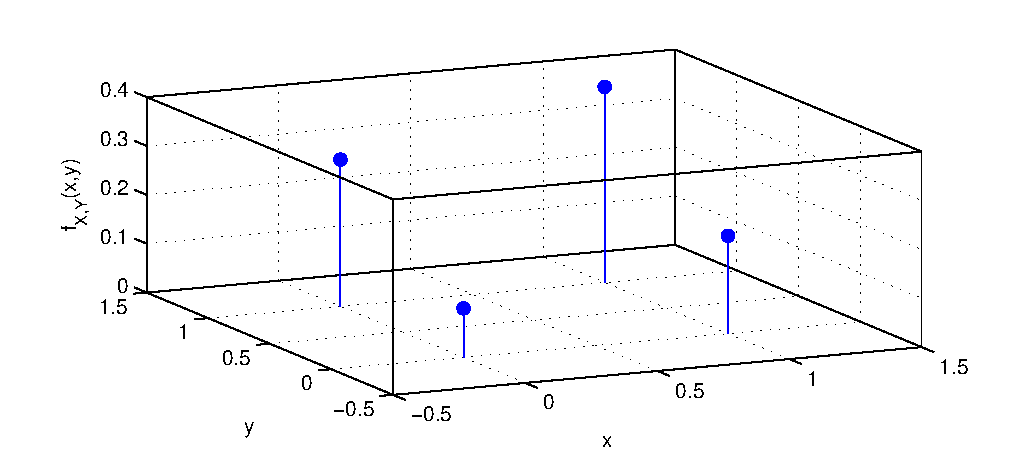
\includegraphics[width=5.0in]{figures/Discrete2DPMF}}
\end{center}
It is helpful to write down the JPMF $f_{X,Y}(x,y)$ in a tabular form:
\begin{center}
\begin{tabular}{|c|c c|}
\hline
& $Y=0$ & $Y=1$ \\ \hline
$X=0$& $0.1$ & $0.3$  \\
$X=1$& $0.2$ & $0.4$  \\ \hline
\end{tabular}
\end{center}
From the above Table we can read for instance that the joint probability $f_{X,Y}(0,0)=0.1$.

Find $\p(B)$ for the event $B=\{(0,0),(1,1)\}$, $F_{X,Y}(1/2,1/2)$, $F_{X,Y}(3/2,1/2)$, $F_{X,Y}(4,5)$ and $F_{X,Y}(-4,-1)$.

\begin{enumerate}
\item $\p(B) = \sum_{(x,y) \in \{(0,0),(1,1)\}}f_{X,Y}(x,y) = f_{X,Y}(0,0)+f_{X,Y}(1,1)=0.1+0.4$
\item $F_{X,Y}(1/2,1/2) = \sum_{\{(x,y): x\leq 1/2, y \leq 1/2\}} f_{X,Y}(x,y)=f_{X,Y}(0,0)=0.1$
\item $F_{X,Y}(3/2,1/2) = \sum_{\{(x,y): x\leq 3/2, y \leq 1/2\}} f_{X,Y}(x,y)=f_{X,Y}(0,0)+f_{X,Y}(1,0)=0.1+0.2=0.3$
\item $F_{X,Y}(4,5) = \sum_{\{(x,y): x\leq 4, y \leq 5\}} f_{X,Y}(x,y)=f_{X,Y}(0,0)+f_{X,Y}(0,1)+f_{X,Y}(1,0)+f_{X,Y}(1,1)=1$
\item $F_{X,Y}(-4,-1) = \sum_{\{(x,y): x\leq -4, y \leq -1\}} f_{X,Y}(x,y)=0$
\end{enumerate}
%\vspace{2cm}
\end{example}

\begin{definition}[JPDF] We say $(X,Y)$ is a {\bf continuous $\R^2$-valued random variable} if its JDF $F_{X,Y}(x,y)$ is differentiable and its {\bf joint probability density function (JPDF)} is given by:
\[
f_{X,Y}(x,y) = \frac{\partial^2}{\partial x \partial y} F_{X,Y}(x,y) \enspace .
\]
\end{definition}

For notational convenience, we sometimes suppress the subscripting when the random variables are clear from the context and write $f(x,y)$ and $F(x,y)$ instead of $f_{X,Y}(x,y)$ and $F_{X,Y}(x,y)$, respectively.

From JPDF $f_{X,Y}$ we can compute the JDF $F_{X,Y}$ at any point $(x,y) \in \Rz^2$ and more generally we can compute the probability of any event $B$, that can be cast as a region in $\Rz^2$, by simply taking two-dimensional integrals:
\begin{equation}\label{Eq:2ContjDFFromjPDF}
\boxed{F_{X,Y}(x,y) = \int_{-\infty}^{y} \int_{-\infty}^{x} f_{X,Y}(u,v) du dv}\enspace ,
\end{equation}
and
\begin{equation}\label{Eq:2ContProbEventFromjPDF}
\boxed{\p(B)\;=\; \int\int_{B} f_{X,Y}(x,y) dx dy}\enspace .
\end{equation}
In particular, if $\Bz_{\delta}(x,y)$ denotes a square of a small area $\delta>0$ that is centered at $(x,y)$, then the following approximate equality holds and improves as $\delta \to 0$:
\begin{equation}\label{Eq:2ContProbEventFromjPDFInSmallBall}
\p\left( (X,Y) \in \Bz_{\delta}(x,y) \right) \approxeq \delta f_{X,Y}(x,y) \enspace .
\end{equation}
The JPDF satisfies the following two properties:
\be
\item integrates to $1$, i.e., $\int_{-\infty}^{\infty} \int_{-\infty}^{\infty} f_{X,Y}(x,y) dx dy=1$
\item is a non-negative function, i.e., $f_{X,Y}(x,y) \geq 0$ for every $(x,y) \in \mathbb{R}^2$.
\ee

\begin{example}\label{Eg:Unif2DPDFandCDF}
Let $(X,Y)$ be a continuous \rv~that is uniformly distributed on the unit square $[0,1]^2 := [0,1] \times [0,1]$ with following JPDF:
\[
f(x,y) =  \BB{1}_{[0,1]^2}(x) 
\begin{cases}
1 & \text{ if } (x,y) \in [0,1]^2 \\
0 & \text{ otherwise}.
\end{cases}
\]
Find explicit expressions for the following: (1) DF $F(x,y)$ for any $(x,y) \in [0,1]^2$, (2) $\p(X \leq 1/3, Y \leq 1/2)$, (3) $P\left( (X,Y) \in [1/4,1/2]\times[1/3,2/3] \right)$.

\begin{center}
\makebox{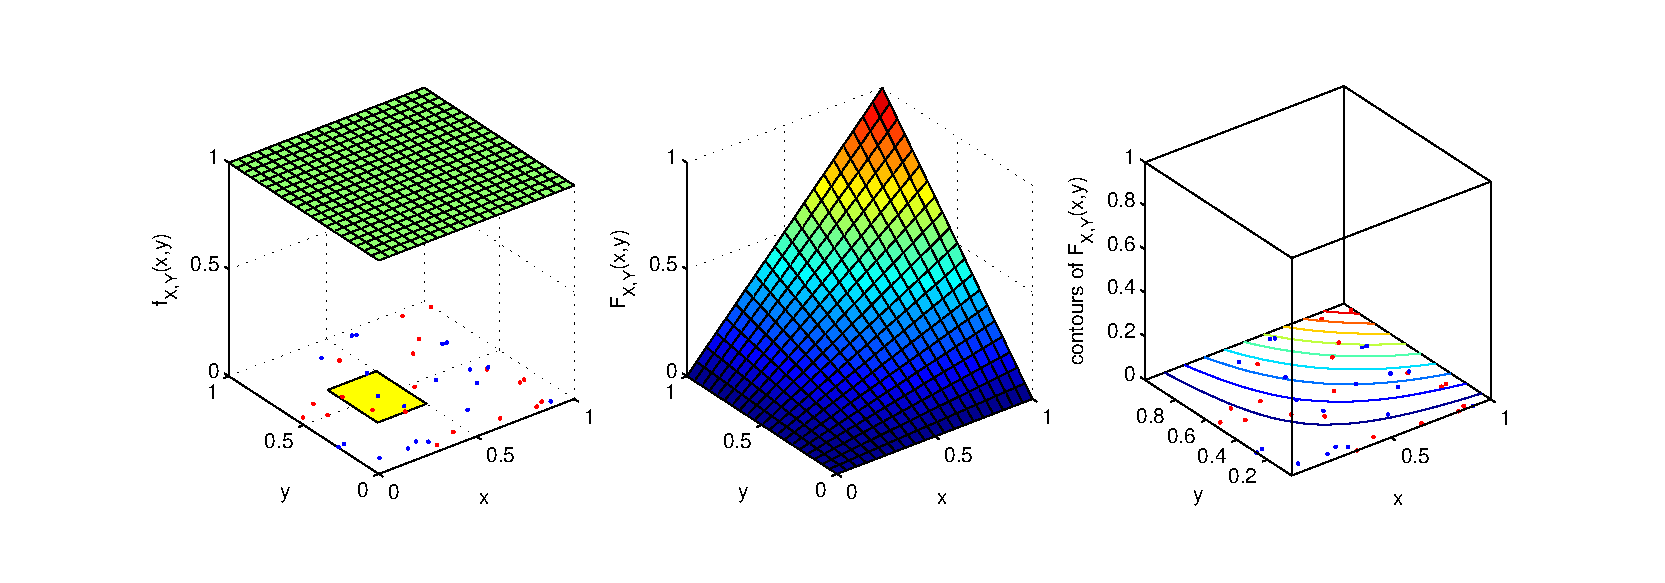
\includegraphics[width=6.5in]{figures/Unif2DPDFandCDF}}
\end{center}

Let us begin to find the needed expressions.
\be
\item
Let $(x,y) \in [0,1]^2$ then by Equation~\eqref{Eq:2ContjDFFromjPDF}:
{\small
\begin{align*}
F_{X,Y}(x,y) 
&= \int_{-\infty}^{y} \int_{-\infty}^{x} f_{X,Y}(u,v) dudv
= \int_{0}^{y} \int_{0}^{{x}} 1 dudv
= \int_{0}^{y} \left[ u \right]_{u=0}^{x}  dv
= \int_{0}^{y} x  dv
&= \left[ x v \right]_{v=0}^{y}
= {x}{y}
\end{align*}
}
\item We can obtain $\p(X \leq 1/3, Y \leq 1/2)$ by evaluating $F_{X,Y}$ at $(1/3,1/2)$:
{\small
\begin{align*}
\p(X \leq 1/3, Y \leq 1/2)
&= F_{X,Y}(1/3,1/2)
= \frac{1}{3}\frac{1}{2}
= \frac{1}{6}
\end{align*}
}
We can also find $\p(X \leq 1/3, Y \leq 1/2)$ by integrating the JPDF over the rectangular event $A=\{X < 1/3, Y < 1/2 \} \subset [0,1]^2$ according to Equation~\eqref{Eq:2ContProbEventFromjPDF}.  
This amounts here to finding the area of $A$, we compute $\p(A) = (1/3) (1/2) = 1/6$.  

\item We can find $P\left( (X,Y) \in [1/4,1/2]\times[1/3,2/3] \right)$ by integrating the JPDF over the rectangular event $B=[1/4,1/2]\times[1/3,2/3]$ according to Equation~\eqref{Eq:2ContProbEventFromjPDF}:
{\small
\begin{align*}
P\left( (X,Y) \in [1/4,1/2]\times[1/3,2/3] \right)
&=\int\int_B f_{X,Y}(x,y)dxdy
=\int_{1/3}^{2/3}\int_{1/4}^{1/2} 1 dx dy\\
&=\int_{1/3}^{2/3} \left[ x \right]_{1/4}^{1/2}  dy
=\int_{1/3}^{2/3} \left[ \frac{1}{2}-\frac{1}{4} \right]  dy
=\left(\frac{1}{2}-\frac{1}{4}\right)\left[ y \right]_{1/3}^{2/3}\\ 
&=\left(\frac{1}{2}-\frac{1}{4}\right)\left( \frac{2}{3}-\frac{1}{3} \right) 
=\frac{1}{4} \left( \frac{1}{3} \right) =\frac{1}{12}
\end{align*}
}
\ee

In general, for a bivariate uniform \rv~on the unit square the $\p([a,b]\times[c,d]) = (b-a)(d-c)$ for any event given by the rectangular region $[a,b]\times[c,d]$ inside the unit square $[0,1]\times[0,1]$.  
Thus any two events with the same rectangular area have the same probability (imagine sliding a small rectangle inside the unit square... no matter where you slide this rectangle to while remaining in the unit square, the probability of $\omega \mapsto (X(\omega),Y(\omega))=(x,y)$ falling inside this ``slidable'' rectangle is the same...).
\end{example}
 
\begin{example}\label{Eg:PlotPDF2ServerTimes}
Let the RV $X$ denote the time until a web server connects to your computer, and let the RV $Y$ denote the time until the server authorizes you as a valid user.  
Each of these RVs measures the waiting time from a common starting time (in milliseconds) and $X < Y$.  
From past response times of the web server we know that a good approximation for the JPDF of the \rv~$(X,Y)$ is
\[
f_{X,Y}(x,y) = 
\begin{cases}
\frac{6}{10^6} \exp \left( -\frac{1}{1000}x-\frac{2}{1000}y \right)
& \text{ if } x>0,y>0,x <y\\
0 & \text{ otherwise}.
\end{cases}
\]
Answer the following:
\be
\item identify the support of $(X,Y)$, i.e., the region in the plane where $f_{X,Y}$ takes positive values
\item check that $f_{X,Y}$ indeed integrates to $1$ as it should
\item Find $\p(X \leq 400, Y \leq 800)$
\item It is known that humans prefer a response time of under $1/10$ seconds ($10^2$ milliseconds) from the web server before they get impatient.  What is $\p(X+Y < 10^2)$? 
\ee
\begin{center}
\makebox{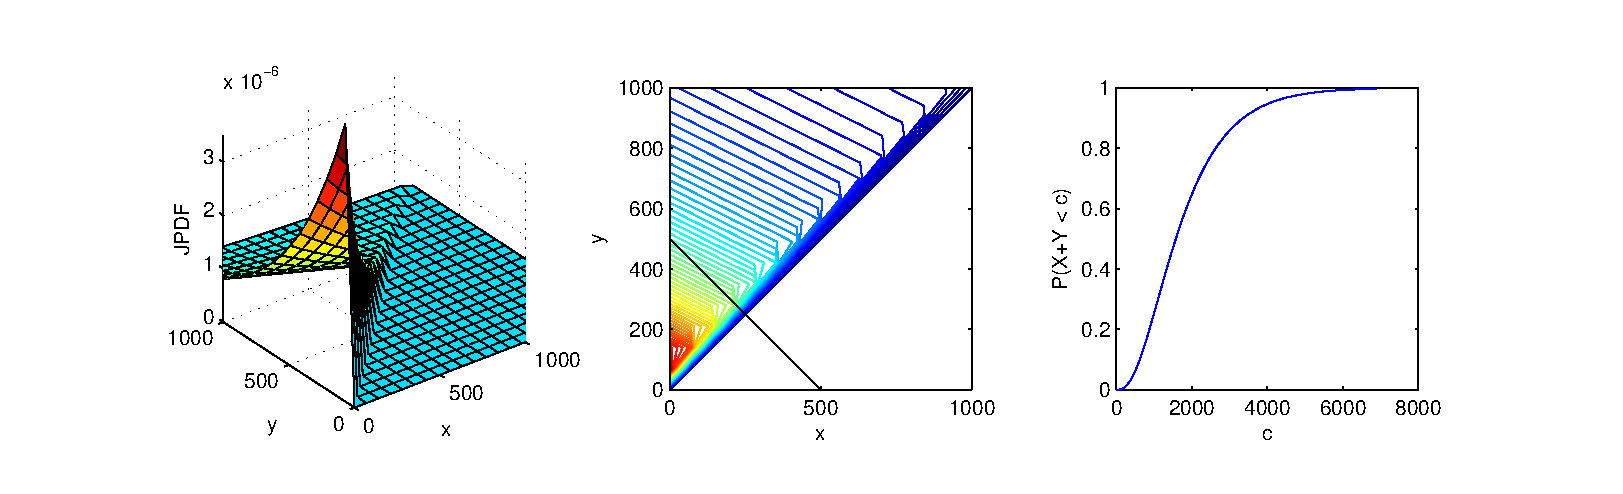
\includegraphics[width=6.0in]{figures/PlotPDF2ServerTimes}}
\end{center}
Let us answer the questions.
\be
\item
The support is the intersection of the positive quadrant with the $y>x$ half-plane.
\item
{\scriptsize
\begin{align*}
\int_{y=-\infty}^{\infty}\int_{x=-\infty}^{\infty} f_{X,Y}(x,y) dx dy 
&= \int_{x=0}^{\infty}\int_{y=x}^{\infty} f_{X,Y}(x,y) dy dx\\
&= \int_{x=0}^{\infty}\int_{y=x}^{\infty} \frac{6}{10^6} \exp \left( -\frac{1}{1000}x-\frac{2}{1000}y \right) dy dx\\
&= \frac{6}{10^6} \int_{x=0}^{\infty} \left(\int_{y=x}^{\infty} \exp \left( -\frac{2}{1000}y \right) dy \right) \exp \left(-\frac{1}{1000}x\right) dx\\
&= \frac{6}{10^6} \int_{x=0}^{\infty} \left[ -\frac{1000}{2} \exp \left( -\frac{2}{1000}y \right) \right]_{y=x}^{\infty}  \exp \left(-\frac{1}{1000}x\right) dx\\
&= \frac{6}{10^6} \int_{x=0}^{\infty} \left[0 +\frac{1000}{2}\exp \left( -\frac{2}{1000}x \right) \right]  \exp \left(-\frac{1}{1000}x\right) dx\\
&= \frac{6}{10^6} \int_{x=0}^{\infty} \frac{1000}{2}\exp \left( -\frac{2}{1000}x -\frac{1}{1000}x\right) dx\\
&= \frac{6}{10^6} \frac{1000}{2} \left[ -\frac{1000}{3} \exp \left(-\frac{3}{1000}x\right)\right]_{x=0}^{\infty} \\
&= \frac{6}{10^6} \frac{1000}{2} \left[0 +\frac{1000}{3} \right] \\
&=1
\end{align*}
}
\item
First, identify the region with positive JPDF for the event $(X \leq 400, Y \leq 800)$
{\scriptsize
\begin{align*}
&\p(X \leq 400, Y \leq 800)\\
&= \int_{x=0}^{400} \int_{y=x}^{800} f_{X,Y}(x,y) dy dx \\
&= \int_{x=0}^{400} \int_{y=x}^{800} \frac{6}{10^6} \exp \left( -\frac{1}{1000}x-\frac{2}{1000}y \right) dy dx \\
&= \frac{6}{10^6}  \int_{x=0}^{400} \left[ -\frac{1000}{2} \exp \left( -\frac{2}{1000}y \right) \right]_{y=x}^{800}  \exp \left(-\frac{1}{1000}x\right) dx\\
&= \frac{6}{10^6} \frac{1000}{2} \int_{x=0}^{400} \left( - \exp \left( -\frac{1600}{1000} \right) + \exp \left( -\frac{2}{1000}x \right) \right)  \exp \left(-\frac{1}{1000}x\right) dx\\
&= \frac{6}{10^6} \frac{1000}{2} \int_{x=0}^{400} \left( \exp \left( -\frac{3}{1000}x \right) - e^{-8/5} \exp \left(-\frac{1}{1000}x\right)\right) dx\\
&= \frac{6}{10^6} \frac{1000}{2} \left( \left( -\frac{1000}{3} \exp \left( -\frac{3}{1000}x \right) \right)_{x=0}^{400} - e^{-8/5} \left(-1000 \exp \left(-\frac{1}{1000}x\right)\right)_{x=0}^{400} \right) \\
&= \frac{6}{10^6} \frac{1000}{2} 1000 \left( \frac{1}{3}\left(1- e^{-6/5} \right) - e^{-8/5} \left( 1-e^{-2/5}\right) \right) \\
&= 3 \left( \frac{1}{3}\left(1- e^{-6/5} \right) - e^{-8/5} \left( 1-e^{-2/5}\right) \right) \\
&\approxeq 0.499 \enspace .
\end{align*}
}
\item
First, identify the region with positive JPDF for the event $(X+Y \leq c)$, say $c=500$ (but generally $c$ can be any positive number).
This is the triangular region at the intersection of the four half-planes: $x>0$, $x < c$, $y>x$ and $y<c-x$. ({\em Draw picture here})
%\vspace{2cm}\\
Let's integrate the JPDF over our triangular event as follows:
{\scriptsize
\begin{align*}
\p(X+Y \leq c) 
&= \int_{x=0}^{c/2}\int_{y=x}^{c-x} f_{X,Y}(x,y) dy dx \\
&= \int_{x=0}^{c/2}\int_{y=x}^{c-x} \frac{6}{10^6} \exp \left( -\frac{1}{1000}x-\frac{2}{1000}y \right) dy dx \\
&= \frac{6}{10^6} \int_{x=0}^{c/2}\int_{y=x}^{c-x}  \exp \left( -\frac{1}{1000}x-\frac{2}{1000}y \right) dy dx \\
&= \frac{6}{10^6} \frac{1000}{2} \int_{x=0}^{c/2} \left[ - \exp \left( -\frac{2}{1000}y \right) \right]_{y=x}^{c-x}  \exp \left(-\frac{1}{1000}x\right) dx\\
&= \frac{3}{10^3} \int_{x=0}^{c/2} \left[ - \exp \left( -\frac{2c-2x}{1000} \right) + \exp \left( -\frac{2x}{1000} \right) \right]  \exp \left(-\frac{x}{1000}\right) dx\\
&= \frac{3}{10^3} \int_{x=0}^{c/2} \left(  \exp \left( -\frac{3x}{1000} \right) - \exp \left( \frac{x-2c}{1000} \right) \right)  dx\\
&= 3 \left( \left[-\frac{1}{3} \exp \left( -\frac{3x}{1000} \right) \right]_{x=0}^{c/2} - \left[ e^{-2c/1000} \exp \left( \frac{x}{1000} \right)\right]_{x=0}^{c/2} \right)  \\
&= 3  \left(\frac{1}{3} (1-e^{-3c/2000}) - e^{-2c/1000} (e^{c/2000}-1) \right)\\
&= 1 - e^{-3c/2000} + 3 e^{-2c/1000} - 3 e^{-3c/2000}\\
&= 1 - 4 e^{-3c/2000} + 3 e^{-c/500}
\end{align*}
}
%\vspace{1cm}\\
\item $\p(X+Y<100) = 1 - 4 e^{-300/2000} + 3 e^{-100/500} \approxeq 0.134$.  This means only about one in one hundred requests to this server will be processed within 100 milliseconds.
\ee
We can obtain $\p(X+Y<c)$ for several values of $c$ using \Matlab and note that about 96\% of requests are processed in less than 3000 milliseconds or 3 seconds.
\begin{VrbM}
>> c = [100 1000 2000 3000 4000]
c =  100        1000        2000        3000        4000

>> p = 1 - 4 * exp(-3*c/2000) + 3 * exp(-c/500)

p =  0.0134     0.5135      0.8558      0.9630      0.9911
\end{VrbM}
\end{example}

\begin{definition}[Marginal PDF or PMF]
If the \rv~$(X,Y)$ has $f_{X,Y}(x,y)$ as its joint PDF or joint PMF, then the 
{\bf marginal PDF or PMF} of a random vector $(X,Y)$ is defined by :
\[
f_{X}(x) =
\begin{cases}
\int_{-\infty}^{\infty} f_{X,Y}(x,y) dy & \text{if $(X,Y)$ is a continuous \rv}  \\
\sum_{y} f_{X,Y}(x,y) & \text{if $(X,Y)$ is a discrete \rv} \\
\end{cases}
\]
and the  {\bf marginal PDF or PMF} of $Y$ is defined by:
\[
f_{Y}(y) = 
\begin{cases}
\int_{-\infty}^{\infty} f_{X,Y}(x,y) dx & \text{if $(X,Y)$ is a continuous \rv}  \\
\sum_{x} f_{X,Y}(x,y) & \text{if $(X,Y)$ is a discrete \rv} \\
\end{cases}
\]
\end{definition}

\begin{example}\label{EgGetMarginalFromJointDiscrete}
Obtain the marginal PMFs $f_Y(y)$ and $f_X(x)$ from the joint PMF $f_{X,Y}(x,y)$ of the discrete \rv~in \hyperref[Eg:Discrete2DPMF]{Example~\ref*{Eg:Discrete2DPMF}}.
Just sum $f_{X,Y}(x,y)$ over $x$'s and $y$'s (reported in a tabular form):
\begin{center}
\begin{tabular}{|c|c c|}
\hline
& $Y=0$ & $Y=1$ \\ \hline
$X=0$& $0.1$ & $0.3$  \\
$X=1$& $0.2$ & $0.4$  \\ \hline
\end{tabular}
\end{center}
From the above Table we can find:
\begin{align*}
f_X(x) = \p(X=x) 
&= \sum_{y} f_{X,Y}(x,y) \\
&= 
f_{X,Y}(x,0) + f_{X,Y}(x,1) = 
\begin{cases}
f_{X,Y}(0,0) + f_{X,Y}(0,1) = 0.1+0.3=0.4 & \text{ if } x=0\\
f_{X,Y}(1,0) + f_{X,Y}(1,1) = 0.2+0.4=0.6 & \text{ if } x=1\\
\end{cases}
\end{align*}
Similarly,
\begin{align*}
f_Y(y) = \p(Y=y) 
&= \sum_{x} f_{X,Y}(x,y) \\
&= 
f_{X,Y}(0,y) + f_{X,Y}(1,y) 
= 
\begin{cases}
f_{X,Y}(0,0) + f_{X,Y}(1,0) = 0.1+0.2=0.3 & \text{ if } y=0\\
f_{X,Y}(0,1) + f_{X,Y}(1,1) = 0.3+0.4=0.7 & \text{ if } y=1\\
\end{cases}
\end{align*}
Just report the marginal probabilities as row and column sums of the JPDF table.

Thus marginal PMF gives us the probability of a specific RV, within a \rv, taking a value irrespective of the value taken by the other RV in this \rv. 
\end{example}

\begin{example}\label{EgGetMarginalFromJointContUnif2DPDFandCDF}
Obtain the marginal PDFs $f_Y(y)$ and $f_X(x)$ from the joint PDF $f_{X,Y}(x,y)$ of the continuous \rv~in \hyperref[Eg:Unif2DPDFandCDF]{Example~\ref*{Eg:Unif2DPDFandCDF}} (the bivariate uniform \rv~on $[0,1]^2$).

\begin{center}
\makebox{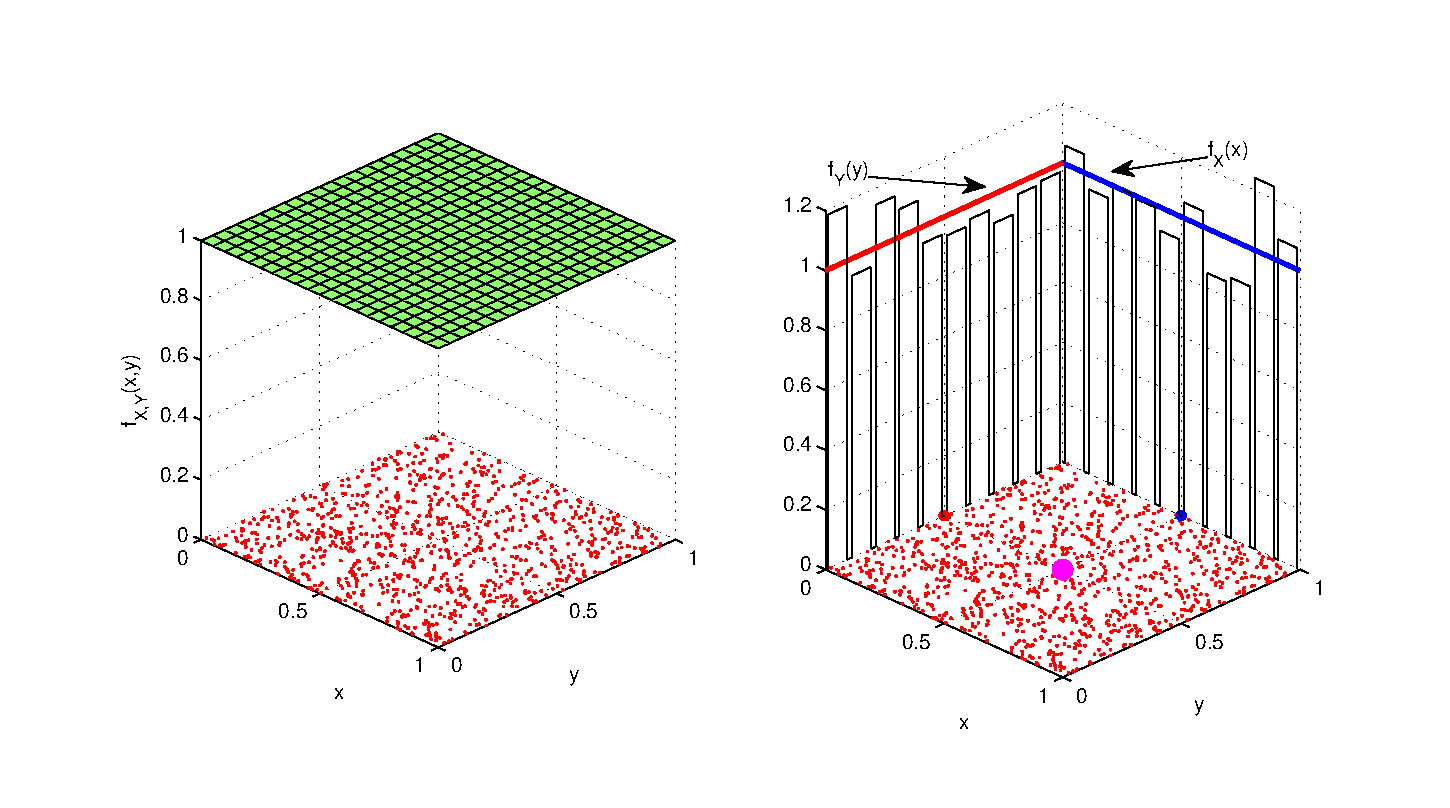
\includegraphics[width=6.0in]{figures/PlotPDFSamplesMarginalsUnif2D}}
\end{center}

Let us suppose $(x,y) \in [0,1]^2$ and note that $f_{X,Y}=0$ if $(x,y) \notin [0,1]^2$.  
We can obtain marginal PMFs $f_X(x)$ and $f_Y(y)$ by integrating the JPDF $f_{X,Y}=1$ along $y$ and $x$, respectively.
\[
f_X(x) = \int_{-\infty}^{\infty} f_{X,Y}(x,y) dy = \int_{0}^{1} f_{X,Y}(x,y) dy 
= \int_{0}^{1} 1 dy = \left[ y \right]_0^1 = 1-0 = 1
\]
Similarly,
\[
f_Y(y) = \int_{-\infty}^{\infty} f_{X,Y}(x,y) dx = \int_{0}^{1} f_{X,Y}(x,y) dx 
= \int_{0}^{1} 1 dx = \left[ x \right]_0^1 = 1-0 = 1
\]
We are seeing a histogram of the {\bf marginal samples} and their marginal PDFs in the Figure.
\end{example}

Thus marginal PDF gives us the probability density of a specific RV in a \rv, irrespective of the value taken by the other RV in this \rv. 

\begin{example}\label{EgGetMarginalFromJointContServerTimes}
Obtain the marginal PDF $f_Y(y)$ from the joint PDF $f_{X,Y}(x,y)$ of the continuous \rv~in \hyperref[Eg:PlotPDF2ServerTimes]{Example~\ref*{Eg:PlotPDF2ServerTimes}} that gave the response times of a web server.
\[
f_{X,Y}(x,y) = 
\begin{cases}
\frac{6}{10^6} \exp \left( -\frac{1}{1000}x-\frac{2}{1000}y \right)
& \text{ if } x>0,y>0,x <y\\
0 & \text{ otherwise}.
\end{cases}
\]
Use $f_Y(y)$ to compute the probability that $Y$ exceeds 2000 milliseconds.

%\vspace{5in}
First we need to obtain an expression for $f_Y(y)$. For $y > 0$,
{\scriptsize
\begin{align*}
f_Y(y) 
&= \int_{x=-\infty}^{\infty} f_{X,Y}(x,y) dx\\
&= \int_{x=-\infty}^{\infty} 6 \times 10^{-6} e^{-0.001 x - 0.002y} dx\\
&= 6 \times 10^{-6} \int_{x=0}^{y} e^{-0.001 x - 0.002y} dx\\ 
&= 6 \times 10^{-6} e^{-0.002y} \int_{x=0}^{y}  e^{-0.001 x} dx\\ 
&= 6 \times 10^{-6} e^{-0.002y} \left[ \frac{e^{-0.001 x}}{-0.001}\right]_{x=0}^{x=y}\\ 
&= 6 \times 10^{-6} e^{-0.002y} \left( \frac{e^{-0.001 y}}{-0.001} - \frac{e^{-0.001 \times 0}}{-0.001} \right)\\ 
&= 6 \times 10^{-6} e^{-0.002y} \left( \frac{1- e^{-0.001 y}}{0.001} \right)\\ 
&= 6 \times 10^{-3} e^{-0.002y} \left({1- e^{-0.001 y}} \right)\\ 
\end{align*}
}
We have the marginal PDF of $Y$ and from this we can obtain 
{\scriptsize
\begin{align*}
\p(Y>2000)
&= \int_{2000}^{\infty} f_Y(y) dy \\
&= \int_{2000}^{\infty} 6 \times 10^{-3} e^{-0.002y} \left({1- e^{-0.001 y}} \right) dy\\
&= 6 \times 10^{-3} \int_{2000}^{\infty}  e^{-0.002y} dy - \int_{2000}^{\infty} e^{-0.003 y} dy\\
&= 6 \times 10^{-3} \left( \left[ \frac{e^{-0.002y}}{-0.002} \right]_{2000}^{\infty} 
- \left( \left[ \frac{e^{-0.003y}}{-0.003} \right]_{2000}^{\infty} \right) \right)\\
&= 6 \times 10^{-3} \left( \frac{e^{-4}}{0.002} - \frac{e^{-6}}{0.003} \right)\\
&= 0.05
\end{align*}
}

{\scriptsize
Alternatively, you can obtain $\p(Y>2000)$ by directly integrating the joint PDF $f_{X,Y}(x,y)$ over the appropriate region (but you may now have to integrate two pieces: rectangular infinite strip ${(x,y): 0<x<2000, y>2000}$ and a triangular infinite piece $\{(x,y): y>x, y>2000, x> 2000\}$)... more involved but we get the same answer.
\begin{multline*}
\p(Y>2000) = \int_{x=0}^{2000} \left( \int_{y=2000}^{\infty} 6 \times 10^{-6} e^{-0.001 x - 0.002y} dy \right) dx + \\
\int_{x=2000}^{\infty} \left( \int_{y=x}^{\infty} 6 \times 10^{-6} e^{-0.001 x - 0.002y} dy \right) dx 
\\
\vdots \text{(try as a tutorial problem)} \\
\p(Y>2000) = 0.0475 + 0.0025 = 0.05
\end{multline*}
}
\end{example}

We have seen the notion of independnece of two events in \hyperref[D:IndOf2Events]{Definition~\ref*{D:IndOf2Events}} or of a sequence of events in \hyperref[D:IndOfSeqOfEvents]{Definition~\ref*{D:IndOfSeqOfEvents}}. 
Recall that independence amounts to having the probability of the joint occurrence of the events to be given by the product of the probabilities of each of the events.

We can use the definition of independence of two events to define the independence of two random variables using their distribution functions.

\begin{definition}[Independence of Two RVs]\label{D:Ind2RVs}
Consider an $\Rz^2$-valued RV $X:=(X_1,X_2)$. Then the $\Rz$-valued RVs $X_1$ and $X_2$ are said to be independent or independently distributed if and only if
\[
\p(X_{1} \leq x_{1}, X_{2} \leq x_{2} ) = \p(X_{1} \leq x_{1}) \p(X_{2} \leq x_{2})
\]
or equivalently,
\[
F_{X_{1},X_{2}}(x_{1},x_{2}) = F_{X_{1}}(x_{1}) F_{X_{2}}(x_{2}) \enspace ,
\]
for any pair of real numbers $(x_{1},x_{2}) \in \Rz^2$.

By the above definition, for {\bf discrete} RVs $X_1,X_2$ that are independent, the following equality is satisfied between the joint and marginal PMFs:
\[
f_{X_1,X_2}(x_1,x_2) = \p(X_{1}= x_{1}, X_{2} = x_{2}) = \p(X_{1} = x_{1}) \p(X_{2} = x_{2}) = f_{X_1}(x_1) f_{X_2}(x_2) \text{ for any} (x_{1},x_{2}) \in \Rz^2 \enspace ,
\]
and for {\bf continuous} RVs $X_1,X_2$ that are independent, the following equality is satisfied between the joint and marginal PDFs:
\[
f_{X_1,X_2}(x_1,x_2) = f_{X_1}(x_1) f_{X_2}(x_2)  \text{ for any} (x_{1},x_{2}) \in \Rz^2 \enspace .
\] 
\end{definition}

In summary, two RVs $X$ and $Y$ are said to be {\bf independent} if and only if for every $(x,y)$
\[
\boxed{
F_{X,Y}(x,y) = F_X(x) \times F_Y(y) \qquad \text{ or } f_{X,Y}(x,y) = f_X(x) \times f_Y(y)
}
\]

Let us confirm that our familiar experiment of tossing a fair coin twice independently when encoded by a pair of independent $\bernoulli(1/2)$ RVs satisfies the above definition.

\begin{example}[Pair of independent $\bernoulli(1/2)$ RVs]\label{EgIndepPairOfBernoulis}
Let $X_1$ and $X_2$ be a pair of independent $\bernoulli(1/2)$ RVs each taking values in the set $\{0,1\}$ with the following tabulated probabilities. Verify that the JPMF $f_{X_1,X_2}(x_1,x_2)=1/4$ for each $(x_1,x_2) \in \{0,1\}^2$ is indeed given by the marginal PMF $f_{X_i}(x_i)=1/2$ for each $i \in \{1,2\}$ and each $x_i \in \{0,1\}$.

\begin{center}
\begin{tabular}{|c|c c|c|}
\hline
& $X_2=0$ & $X_2=1$ & \\ \hline
$X_1=0$& $1/4$ & $1/4$ & $1/2$ \\
$X_1=1$& $1/4$ & $1/4$ & $1/2$ \\ \hline
& $1/2$ & $1/2$ & $1$\\ \hline
\end{tabular}
\end{center}
From the above Table we can read for instance that the {\em joint probability} that $\Rz^2$-valued RV $(X_1,X_2)$ takes the value or realization $(0,0)$ is $1/4$ from the first entry of the inner-most tabulated rectangle, 
i.e., $\p((X_1,X_2)=(0,0))=1/4$, 
and that the {\em marginal probability} that the RV $X_1$ takes the value or relaization $0$ is $1/2$, 
i.e., $\p(X_1=0)=1/2$. 
Clearly, $1/4=1/2 \times 1/2$, and so our familiar experiment when seen as an $\Rz^2$-valued RV is indeed composed of two independent$\Rz$-valued $\bernoulli(1/2)$ RVs. 
\end{example}

\begin{example}\label{EgShowIndepUnifDensityOnUnitSquare}
Recall the $\Rz^2$-valued continuous RV $(X,Y)$ of \hyperref[Eg:Unif2DPDFandCDF]{Example~\ref*{Eg:Unif2DPDFandCDF}} 
that is uniformly distributed on the unit square $[0,1]^2$. 
First show that $X$ and $Y$ independent. 
Then show that both $X$ and $Y$ are identically distributed according to the $\uniform(0,1)$ RV. 

{\em Solution:}\\[4pt]
This can be shown by checking that the joint PDF is indeed equal to the product of the marginal PDFs of $\uniform(0,1)$ RVs as follows:
\[
\begin{cases}
1= f_{X,Y}(x,y) =  f_X(x) \times f_Y(y) = 1 \times 1 = 1 & \text{ if } (x,y) \in [0,1]^2\\
0= f_{X,Y}(x,y) =  f_X(x) \times f_Y(y) = 0 \times 0 = 0 & \text{ if } (x,y) \notin [0,1]^2
\end{cases}
\]
\end{example}

Are $X$ and $Y$ independent in the server times \rv~from \hyperref[Eg:PlotPDF2ServerTimes]{Example~\ref*{Eg:PlotPDF2ServerTimes}}?

We can compute $f_X(x)$ and use the already computed $f_Y(y)$ to mechanically check if the JPDF is the product of the marginal PDFs.  But intuitively, we know that these RVs (connection time and authentication time) are dependent -- one is strictly greater than the other.  
Also the JPDF has zero density when $x>y$, but the product of the marginal densities won't.

Now, let us take advantage of independent random variables and solve some problems.

\begin{example}[distance between random faults in a manufactured line]\label{EgDistBetweenFaultsOnLine}
Suppose two points are tossed independently and uniformly at random onto a line segment of unit length.  
What is the probability that the distance between the two points does not exceed a given length $l$? 

\vspace{5cm}
done in lectures...

\end{example}

\begin{example}[Buffon's Needle Experiment to Physically Estimate $\pi$]\label{EgBuffonsNeedle}
Suppose a needle is tossed at random onto a plane ruled with parallel lines a distance $L$ apart. 
By a ``needle'' we mean a line segment of length $ l \leq L$.

What is the probability that the needle intersects one of the parallel lines? Can you use repeated trials of this experiment to find an approximation to $\pi$?

{\em Solution:}\\[4pt]
Let $X_1$ be the angle between the needle and the direction of the rulings, and let $X_2$ be the distance between the bottom point of the needle and the nearest line above this point (see left sub-figure of Figure~\ref{F:BuffonsNeedle}). 
Then the conditions of the ``needle tossing at random'' experiment are such that the RV $X_1$ is uniformly distributed in the interval $[0,\pi]$, while the RV $X_2$ is uniformly distributed in the interval $[0,L]$. 
Hence {\em assuming that the RVs $X_1$ and $X_2$ are independent}, we find that their joint probability density function (JPDF) is:
\[
f_{X_1,X_2}(x_1,x_2) = \frac{1}{\pi}\BB{1}_{[0,\pi]}(x_1) \times \frac{1}{L}\BB{1}_{[0,L]}(x_2) = \frac{1}{\pi L} \BB{1}_{[0,\pi]}(x_1) \BB{1}_{[0,L]}(x_2) = \frac{1}{\pi L} \BB{1}_{[0,\pi] \times [0,L] }(x_1,x_2) \enspace . 
\]
The event $A$ that the needle intersects one of the parallel ruled lines occurs if and only if
\[
X_2 \leq l \sin(X_1) \enspace,
\]
i.e., if and only if the corresponding point $X := (X_1,X_2)$ falls in the region $B$, where $B$ is part of the rectangle $[0,\pi] \times [0,L]$ lying between the $x_1$-axis and the curve $x_2=\sin(x_1)$ (area under the curve in right-subfigure of Figure~\ref{F:BuffonsNeedle}). 
Hence, we can integrate the JPDF to get the probability of the event $A$ of interest:
\[
\p(A) = \p \left( (X_1,X_2) \in B \right) = \underset{B}{\int \int} \frac{dx_1 dx_2}{\pi L} = \frac{2l}{\pi L}
\]
where,
\[
l \int_0{\pi} \sin(x_1) dx_1 = l \left( - \cos(x_1)\right]_0^{\pi} = l(1-(-1))=l(1+1)=2l \enspace,
\]
is the area of $B$. 

Thus, if the needle is repeatedly tossed onto the ruled plane and $n(A)$ is the number of times $A$ occurs out of $n$ trials, then the relative frequency of the event $A$ should approach $\p(A)$ as $n \to \infty$ (we will see this as the Law of Large Numbers in the sequel, but recall that this is also how we motivated the LTRF or long-term relative frequency idea of probability):
\[
\frac{n(A)}{n} \to \frac{2l}{\pi L}
\]
Hence, for large $n$,
\[
\frac{2 l}{L}\frac{n}{n(A)}
\]
should be a good approximation to $\pi=3.14\ldots$. This is indeed the case.
\end{example}
\begin{figure}
\vspace{3cm}
\caption{Diagrams done on the board! \label{F:BuffonsNeedle}}
\end{figure}

\subsection{Conditional Random Variables}\label{S:CondRVs}

Often we will have a condition where one of the two random variables that make up a random vector $(X_1,X_2)$ already occurs and takes a value. 
And we might want to compute the probability of the occurrence of the other random variable given this conditional information.
For this all we need to do is extend the idea of conditional probabiliies to $\Rz^2$-valued random variables as defined below.

\begin{definition}[Conditional PDF or PMF]
Let $(X_1,X_2)$ be a discrete bivariate \rv.  The conditional PMF of $X_1|X_2=x_2$, where $f_{X_2}(x_2) := \p(X_2=x_2) > 0$ is:
\[
f_{X_1|X_2}(x_1 | x_2) := \p(X_1=x_1 | X_2=x_2) = \frac{\p(X_1=x_1,X_2=x_2)}{\p(X_2=x_2)} = \frac{f_{X_1,X_2}(x_1,x_2)}{f_{X_2}(x_2)} \ .
\]
Similarly, if $f_{X_1}(x_1) := \p(X_1=x_1) >0$, then the conditional PMF of $X_2|X_1=x_1$ is:
\[
f_{X_2|X_1}(x_2|x_1) := \p(X_2=x_2 | X_1=x_1) = \frac{\p(X_1=x_1,X_2=x_2)}{\p(X_1=x_1)} = \frac{f_{X_1,X_2}(x_1,x_2)}{f_{X_1}(x_1)} \ .
\]
If $(X_1,X_2)$ are continuous RVs such that the marginal PDF $f_{X_2}(x_2)>0$, then the conditional PDF of $X_1|X_2=x_2$ is:
\[
f_{X_1|X_2}(x_1|x_2) = \frac{f_{X_1,X_2}(x_1,x_2)}{f_{X_2}(x_2)}, \qquad \p(X_1 \in A| X_2=x_2) = \int_A f_{X_1|X_2}(x_1|x_2) dx_1 \ .
\]
Similarly, if $f_{X_1}(x_1)>0$, then the conditional PDF of $X_2|X_1=x_1$ is:
\[
f_{X_2|X_1}(x_2|x_1) = \frac{f_{X_1,X_2}(x_1,x_2)}{f_{X_1}(x_1)}, \qquad \p(X_2 \in A| X_1=x_1) = \int_A f_{X_2|X_1}(x_2|x_1) dx_2 \ .
\]
\end{definition}

Let us consider a few discrete RVs for the simple coin tossing experiment $\E{E}_{\theta}^{3}$ that build on the $\bernoulli(\theta)$ RV $X_i$ for the $i$-th toss in an {\bf independent and identically distibuted (IID.)} manner.
\begin{table}[htpb]
\caption{The $8$ $\omega$'s in the sample space $\Omega$ of the experiment $\E{E}_{\theta}^{3}$ are given in the first row above.  The RV $Y$ is the number of `Heads' in the $3$ tosses and the RV $Z$ is the number of `Tails' in the $3$ tosses.  Finally, the RVs $Y'$ and $Z'$ are the indicator functions of the event that `all three tosses were Heads' and the event that `all three tosses were Tails', respectively.\label{T:T3XRVs}}
 \begin{tabular}{r c c c c c c c c l}
 \hline
$\omega$:    & {\tt HHH} & {\tt HHT} & {\tt HTH} & {\tt HTT} & {\tt THH} & {\tt THT} & {\tt TTH} & {\tt TTT} & RV Definitions / Model \\ \hline
 \\
$\p(\omega)$: & $\frac{1}{8}$ & $\frac{1}{8}$ & $\frac{1}{8}$ & $\frac{1}{8}$ &  $\frac{1}{8}$ & $\frac{1}{8}$ & $\frac{1}{8}$ & $\frac{1}{8}$  & $X_i \overset{\IID}{\sim} \bernoulli(\frac{1}{2})$ \\
 \\
$Y(\omega)$: & 3         & 2         & 2         & 1         & 2         & 1         & 1         & 0        & $Y := X_1+X_2+X_3$ \\
 \\
$Z(\omega)$: & 0         & 1         & 1         & 2         & 1         & 2         & 2         & 3        & $Z := (1-X_1)+(1-X_2)+(1-X_3)$ \\
 \\
$Y'(\omega)$: & 1         & 0         & 0         & 0         & 0         & 0         & 0         & 0       & $Y' :=  X_1 X_2 X_3$ \\
\\
$Z'(\omega)$: & 0         & 0         & 0         & 0         & 0         & 0         & 0         & 1       & $Y' :=  (1-X_1)(1-X_2)(1-X_3)$ \\ \hline
 \end{tabular}
 \end{table}
 \begin{classwork}[Two random variables of `toss a coin thrice' experiment]
Describe the probability of the RV $Y$ and $Y'$ of \hyperref[T:T3XRVs]{Table \ref*{T:T3XRVs}} in terms of its PMF.  Repeat the process for the RV $Z$ in your spare time.
 \begin{eqnarray}
 \p(Y=y) =%:= \p(\{\omega: Y(\omega)=y\}) = 
 \begin{cases}
 \qquad & \qquad \notag \\
 \qquad & \qquad \notag \\
 \qquad & \qquad \notag \\
 \qquad & \qquad \notag
 \end{cases} 
 & \qquad \qquad \qquad \qquad \qquad
\p(Y'=y') =%:= \p(\{\omega: Y'(\omega)=y'\}) = 
 \begin{cases}
 \qquad & \qquad \notag \\
 \qquad & \qquad \notag 
 \end{cases}
 \end{eqnarray}
 \end{classwork}
 
 \begin{classwork}[The number of `Heads' given there is at least one `Tails']
 Consider the following two questions.
 \begin{enumerate}
\item What is conditional probability $\p(Y|Y'=0)$ ?
%{\color{Gray}{
 \[
 \begin{array}{c c c c}
 \hline \\
 \p(Y=y | Y'=0) & =\frac{\p(Y=y,Y'=0)}{\p(Y'=0)} & =\frac{\p(\{\omega: Y(\omega)=y \  \cap \ Y'(\omega)=0\})}{\p(\{\omega: Y'(\omega)=0\})} & = ? \\ \hline \\
 \\
 \p(Y=0 | Y'=0) & \frac{\p(Y=0,Y'=0)}{\p(Y'=0)} & \frac{\frac{1}{8}}{\frac{1}{8}+\frac{1}{8}+\frac{1}{8}+\frac{1}{8}+\frac{1}{8}+\frac{1}{8}+\frac{1}{8}} & \frac{1}{7} \\
\\
\p(Y=1 | Y'=0) & \frac{\p(Y=1,Y'=0)}{\p(Y'=0)} & \frac{\frac{1}{8}+\frac{1}{8}+\frac{1}{8}}{\frac{1}{8}+\frac{1}{8}+\frac{1}{8}+\frac{1}{8}+\frac{1}{8}+\frac{1}{8}+\frac{1}{8}} & \frac{3}{7} \\
\\
\p(Y=2 | Y'=0) & \frac{\p(Y=2,Y'=0)}{\p(Y'=0)} & \frac{\frac{1}{8}+\frac{1}{8}+\frac{1}{8}}{\frac{1}{8}+\frac{1}{8}+\frac{1}{8}+\frac{1}{8}+\frac{1}{8}+\frac{1}{8}+\frac{1}{8}} & \frac{3}{7} \\
\\
\p(Y=3 | Y'=0) & \frac{\p(Y=3,Y'=0)}{\p(Y'=0)} & \frac{\p(\emptyset)}{\frac{1}{8}+\frac{1}{8}+\frac{1}{8}+\frac{1}{8}+\frac{1}{8}+\frac{1}{8}+\frac{1}{8}} & 0 \\
\\ \hline
\p(Y \in \{0,1,2,3\} | Y'=0) & \frac{\sum_{y=0}^3{\p(Y=y,Y'=0)}}{\p(Y'=0)} & \frac {\frac{1}{8}+\frac{1}{8}+\frac{1}{8}+\frac{1}{8}+\frac{1}{8}+\frac{1}{8}+\frac{1}{8}}{\frac{1}{8}+\frac{1}{8}+\frac{1}{8}+\frac{1}{8}+\frac{1}{8}+\frac{1}{8}+\frac{1}{8}} & 1 \\ \hline
 \end{array}
 \]
% }}
\item What is $\p(Y|Y'=1)$ ?
%{\color{Gray}{
 \[
\p(Y=y | Y'=1) = 
\begin{cases}
1 & \text{if $y=3$} \\
0 & \text{otherwise}
 \end{cases}
 \]
 %}}
 \end{enumerate}
 \end{classwork}

\subsection{$\Rz^m$-valued Random Variables}\label{S:Rm-valuedRVs}

%Extension to multivariate random vectors that are made of more than two RVs is straightforward.  
Consider the \rv~ $X$ whose components are the RVs $X_1,X_2,\ldots,X_m$, i.e., $X := (X_1,X_2,\ldots,X_m)$, where $m \geq 2$.  
A particular realization of this RV is a point $(x_1,x_2,\ldots,x_m)$ in $\Rz^m$.  
Now, let us extend the notions of JCDF, JPMF and JPDF to $\Rz^m$.  

\begin{definition}[multivariate JDF]\label{Df:JmDF}
The {\bf joint distribution function (JDF)} or {\bf joint cumulative distribution function (JCDF)}, $F_{X_1,X_2,\ldots,X_m}(x_1,x_2,\ldots,x_m):\mathbb{R}^m\to [0,1]$, of the multivariate random vector $(X_1,X_2,\ldots,X_m)$ is
\begin{eqnarray}\label{E:jmDF}
F_{X_1,X_2,\ldots,X_m}(x_1,x_2,\ldots,x_m)\; 
&=& \p(X\leq x_1 \cap X_2 \leq x_2 \cap \cdots \cap X_m \leq x_m)\notag\\ 
&=& \p(X_1\leq x_1 , X_2 \leq x_2, \ldots, X_m \leq x_m)\\
&=& P\left( \{ \omega: X_1(\omega) \leq x_1, X_2(\omega) \leq x_2, \ldots, X_m(\omega) \leq x_m \} \right), \notag
\end{eqnarray}
for any $(x_1,x_2,\ldots,x_m) \in \mathbb{R}^m$, 
where the right-hand side represents the probability that the random vector $(X_1,X_2,\ldots,X_m)$ takes on a value in 
$\{(x'_1,x'_2,\ldots,x'_m): x'_1 \leq x_1, x'_2 \leq x_2, \ldots, x'_m \leq x_m\}$, the set of points in $\Rz^m$ that are less than the point $(x_1,x_2,\ldots,x_m)$ in each coordinate $1,2,\ldots,m$.
\end{definition}

The JDF $F_{X_1,X_2,\ldots,X_m}(x_1,x_2,\ldots,x_m):\Rz^m\to\Rz$ satisfies the following conditions to remain a probability: 
\begin{enumerate}
\item $0 \leq F_{X_1,X_2,\ldots,X_m}(x_1,x_2,\ldots,x_m) \leq 1$
\item $F_{X_1,X_2,\ldots,X_m}(x_1,x_2,\ldots,x_m)$ is an increasing function of $x_1$, $x_2$, $\ldots$ and $x_m$
\item $F_{X_1,X_2,\ldots,X_m}(x_1,x_2,\ldots,x_m) \to 1$ as $x_1\to \infty$, $x_2\to \infty$, $\ldots$ and $x_m\to \infty$
\item $F_{X_1,X_2,\ldots,X_m}(x_1,x_2,\ldots,x_m) \to 0$ as $x_1\to -\infty$, $x_2\to -\infty$, $\ldots$ and $x_m\to -\infty$
\end{enumerate}

\begin{definition}[Multivariate JPMF]
If $(X_1,X_2,\ldots,X_m)$ is a {\bf discrete random vector} that takes values in a discrete support set $\mathcal{S}_{X_1,X_2,\ldots,X_m}$, then its \textbf{joint probability mass function} (or JPMF) is:
\begin{equation}\label{Eq:jmDPMF}
f_{X_1,X_2,\ldots,X_m}(x_1,x_2,\ldots,x_m) = \p(X_1=x_1,X_2=x_2,\ldots,X_m=x_m) \enspace . 
\end{equation}
\end{definition}
Since $\p(\Omega)=1$, $\sum_{{\substack{(x_1,x_2,\ldots,x_m) \in \mathcal{S}_{X_1,X_2,\ldots,X_m}}}}f_{X_1,X_2,\ldots,X_m}(x_1,x_2,\ldots,x_m)=1$.

From JPMF $f_{X_1,X_2,\ldots,X_m}$ we can get the JCDF $F_{X_1,X_2,\ldots,X_m}(x_1,x_2,\ldots,x_m)$ and the probability of any event $B$ by simply taking sums as in Equation~\eqref{Eq:2DiscretejDFFromjPMF} but now over all $m$ coordinates.
%\begin{equation}\label{Eq:2DiscretejDFFromjPMF}
%\boxed{F_{X_1,X_2,\ldots,X_m}(x,y)\;=\;\sum_{x_i\leq x, y_j \leq y}f_{X_1,X_2,\ldots,X_m}(x_i,y_j) }\enspace ,
%\qquad \boxed{\p(B)\;=\;\sum_{\substack{(x_i, y_j) \in B \cap \mathcal{S}_{X_1,X_2,\ldots,X_m}}}f_{X_1,X_2,\ldots,X_m}(x_i,y_j) }\enspace ,
%\end{equation}

\begin{definition}[Multivariate JPDF]
$(X_1,X_2,\ldots,X_m)$ is a {\bf continuous random vector} if its JDF $F_{X_1,X_2,\ldots,X_m}(x_1,x_2,\ldots,x_m)$ is differentiable and the {\bf joint probability density function (JPDF)} is given by:
\[
f_{X_1,X_2,\ldots,X_m}(x_1,x_2,\ldots,x_m) = \frac{\partial^m}{\partial x_1 \partial x_2 \cdots \partial x_m} F_{X_1,X_2,\ldots,X_m}(x_1,x_2,\ldots,x_m) \enspace ,
\]
\end{definition}

From JPDF $f_{X_1,X_2,\ldots,X_m}$ we can compute the JDF $F_{X_1,X_2,\ldots,X_m}$ at any point $(x_1,x_2,\ldots,x_m) \in \Rz^m$ and more generally we can compute the probability of any event $B$, that can be cast as a region in $\Rz^m$, by ``simply'' taking $m$-dimensional integrals (you have done such iterated integrals when $m=3$):
\begin{equation}\label{Eq:mContjDFFromjPDF}
\boxed{F_{X_1,X_2,\ldots,X_m}(x_1,x_2,\ldots,x_m) = \int_{-\infty}^{x_m} \cdots \int_{-\infty}^{x_2} \int_{-\infty}^{x_1} f_{X_1,X_2,\ldots,X_m}(x_1,x_2,\ldots,x_m) dx_1 dx_2\ldots d x_m}\enspace ,
\end{equation}
and
\begin{equation}\label{Eq:mContProbEventFromjPDF}
\boxed{\p(B)\;=\; \int\cdots\int\int_{B} f_{X_1,X_2,\ldots,X_m}(x_1,x_2,\ldots,x_m) dx_1 dx_2\ldots d x_m}\enspace .
\end{equation}
The JPDF satisfies the following two properties:
\be
\item integrates to $1$, i.e., $\int_{-\infty}^{\infty} \cdots \int_{-\infty}^{\infty}\int_{-\infty}^{\infty} f_{X_1,X_2,\ldots,X_m}(x_1,x_2,\ldots,x_m) dx_1 dx_2\ldots d x_m=1$
\item is a non-negative function, i.e., $f_{X_1,X_2,\ldots,X_m}(x_1,x_2,\ldots,x_m) \geq 0$.
\ee

The marginal PDF (marginal PMF) is obtained by integrating (summing) the JPDF (JPMF) over all other random variables.  
For example, the marginal PDF of $X_1$ is
\[
f_{X_1}(x_1) =
\int_{x_2=-\infty}^{\infty}\cdots \int_{x_m=-\infty}^{\infty} f_{X_1,X_2,\ldots,X_m}(x_1,x_2,\ldots,x_m) dx_2\ldots d x_m 
\]

\begin{definition}[Independence of Sequence of RVs]\label{D:IndRVs}
A finite or infinite sequence of RVs $X_1,X_2,\ldots$ is said to be independent or independently distributed if and only if
\[
\p(X_{i_1} \leq x_{i_1}, X_{i_2} \leq x_{i_2}, \ldots,  X_{i_k} \leq x_{i_k} ) = \p(X_{i_1} \leq x_{i_1}) \p(X_{i_2} \leq x_{i_2}) \cdots,  \p(X_{i_k} \leq x_{i_k} )
\]
or equivalently,
\[
F_{X_{i_1},X_{i_2},\ldots,X_{i_m}}(x_{i_1},x_{i_2},\ldots,x_{i_m}) = F_{X_{i_1}}(x_{i_1}) F_{X_{i_2}}(x_{i_2}) \cdots F_{X_{i_m}}(x_{i_m}) \enspace ,
\]
for any distinct subset of indices $\{i_1,i_2,\ldots,i_m\}$ of $\{1,2,\ldots\}$, the index set of the sequence of RVs and any sequence of real numbers $x_{i_1},x_{i_2},\ldots,x_{i_m}$.

By the above definition, the sequence of {\bf discrete} RVs $X_1,X_2,\ldots$ taking values in an at most countable set $\Dz$ are said to be independently distributed if for any distinct subset of indices $\{i_1,i_2,\ldots,i_k\}$ such that the corresponding RVs $X_{i_1},X_{i_2},\ldots,X_{i_k}$ exists as a distinct subset of our original sequence of RVs $X_1,X_2,\ldots$ and for any elements $x_{i_1}, x_{i_2},\ldots,x_{i_k}$ in $\Dz$, the following equality is satisfied:
\[
\p(X_{i_1}= x_{i_1}, X_{i_2} = x_{i_2}, \ldots,  X_{i_k} = x_{i_k} ) = \p(X_{i_1} = x_{i_1}) \p(X_{i_2} = x_{i_2}) \cdots  \p(X_{i_k} = x_{i_k}) \enspace ,
\]
or equivalently,
\[
f_{X_{i_1}, X_{i_2},\ldots,X_{i_k}} (x_{i_1}, x_{i_2}, \ldots,  x_{i_k} ) = f_{X_{i_1}} (x_{i_1}) f_{X_{i_2}}(x_{i_2}) \cdots  f_{X_{i_k}} (x_{i_k}) \enspace .
\]
\end{definition}

From Definition~\ref{D:IndRVs}, we say $m$ random variables $X_1,X_2,\ldots,X_m$ are jointly independent or mutually independent if and only if for every $(x_1,x_2,\ldots,x_m) \in \Rz^m$
\begin{eqnarray}
F_{X_{1},X_{2},\ldots,X_{m}}(x_{1},x_{2},\ldots,x_{m}) &=& F_{X_{1}}(x_{1}) F_{X_{2}}(x_{2}) \cdots F_{X_{m}}(x_{m}) \enspace ,\\
f_{X_{1},X_{2},\ldots,X_{m}}(x_{1},x_{2},\ldots,x_{m}) &=& f_{X_{1}}(x_{1}) f_{X_{2}}(x_{2}) \cdots f_{X_{m}}(x_{m}) \enspace .
\end{eqnarray}

\begin{prop}[Conditional probability of independent sequence of RVs]
For an independent sequence of RVs $\{X_1,X_2,\ldots\}$, we have
\begin{equation}\label{Eqn:CndProbOfIndepSeqOfRVs}
\p(X_{i+1} \leq x_{i+1} | X_{i} \leq x_{i}, X_{i-1} \leq x_{i-1}, \ldots, X_1 \leq x_1) =  \p(X_{i+1} \leq x_{i+1}) 
\end{equation}
\end{prop}
\begin{proof}
\begin{eqnarray}
&&\p(X_{i+1} \leq x_{i+1} | X_{i} \leq x_{i}, X_{i-1} \leq x_{i-1}, \ldots, X_1 \leq x_1) \notag\\
\notag \\
&=& \frac{\p(X_{i+1} \leq x_{i+1}, X_{i} \leq x_{i}, X_{i-1} \leq x_{i-1}, \ldots, X_1 \leq x_1)}{\p(X_{i} \leq x_{i}, X_{i-1} \leq x_{i-1}, \ldots, X_1 \leq x_1)} \notag \\
\notag \\
&=& \frac{\p(X_{i+1} \leq x_{i+1}) \p(X_{i} \leq x_{i}) \p(X_{i-1} \leq x_{i-1}) \cdots \p(X_1 \leq x_1)}{\p(X_{i} \leq x_{i}) \p(X_{i-1} \leq x_{i-1}) \cdots \p(X_1 \leq x_1)} \notag \\
\notag \\
&=& \p(X_{i+1} \leq x_{i+1}) \notag 
\end{eqnarray}
\end{proof}
Equation~\eqref{Eqn:CndProbOfIndepSeqOfRVs} simply says that the conditional distribution of the RV $X_{i+1}$ given all previous RVs $X_i,X_{i-1},\ldots,X_1$ is simply determined by the distribution of $X_{i+1}$.

\begin{example}\label{EgCovOf2IndepRVs}
If $X_1$ and $X_2$ are independent random variables then what is their covariance $\cv(X_1,X_2)$?

{\em Solution:}\\[4pt]
We know for independent RVs from the properties of expectations that
\[
E(X_1X_2) = E(X_1)E(X_2)
\]
From the formula for covariance
\begin{align*}
\cv (X_1,X_2) 
&= E(X_1 X_2)-E(X_1)E(X_2)\\
&= E(X_1) E(X_2)-E(X_1)E(X_2) \qquad \text{due to independence}\\
&= 0
\end{align*}
\end{example}

\begin{rem}
The converse is not true: two random variables that have zero covariance are not necessarily independent.
\end{rem}

\subsubsection{Linear Combination of Independent Normal RVs is a Normal RV}

We can get the following special property of normal RVs using Eqn.~\eqref{E:LinCombCF}. 
If $X_1,X_2,\ldots,X_m$ be jointly independent RVs, where $X_i$ is $\normal(\mu_i,\sigma_i^2)$, for $i=1,2,\ldots,m$ 
then $Y=c+\sum_{i=1}^m a_i X_i$ for some constants $c,a_1,a_2,\ldots,a_m$ 
is the $\normal\left( c+\sum_{i=1}^m a_i \mu_i, \sum_{i=1}^m a_i^2 \sigma_i^2 \right)$ RV.

\begin{example}\label{EgLinCombOfNormals}
Let $X$ be $\normal(2,4)$, $Y$ be $\normal(-1,2)$ and $Z$ be $\normal(0,1)$ RVs that are jointly independent.  
Obtain the following:
\be
\item $E(3X-2Y+4Z)$
\item $V(2Y-3Z)$
\item the distribution of $6-2Z+X-Y$
\item the probability that $6-2Z+X-Y>0$
\item $\cv(X,W)$, where $W=X-Y$.
\ee

{\em Solution}\\[4pt]
\be
\item
\[
E(3X-2Y+4Z) = 3E(X)-2E(Y)+4(Z) = (3 \times 2) + (-2 \times (-1)) + 4 \times 0 = 6 +2 +0 = 8
\]
\item
\[
V(2Y-3Z) = 2^2V(Y) + (-3)^2V(Z) = (4 \times 2) + (9 \times 1) = 8 + 9 = 17 
\]
\item
From the special property of normal RVs, the distribution of $6-2Z+X-Y$ is
\begin{align*}
&~ \normal\left( 6+(-2 \times 0)+(1 \times 2)+(-1 \times -1), ((-2)^2 \times 1) + (1^2 \times 4) + ((-1)^2 \times 2)  \right)\\
&= \normal\left( 6+0+2+1, 4 + 4 +  2  \right)\\
&= \normal(9,10)
\end{align*}
\item 
Let $U=6-2Z+X-Y$ and we know $U$ is $\normal(9,10)$ RV.
\begin{align*}
P(6-2Z+X-Y>0) 
&= P(U>0) = P(U-9>0-9) = P\left( \frac{U-9}{\sqrt{10}} > \frac{-9}{\sqrt{10}} \right)\\
&= P\left( Z > \frac{-9}{\sqrt{10}} \right)\\ 
&= P\left( Z < \frac{9}{\sqrt{10}} \right) \\
&\approxeq P(Z < 2.85) = 0.9978
\end{align*}
\item
\begin{align*}
\cv(X,W) 
&= E(XW)-E(X)E(W) = E(X(X-Y))-E(X)E(X-Y)\\
&= E(X^2-XY)-E(X)(E(X)-E(Y)) = E(X^2)-E(XY)-2\times(2-(-1)) \\
&= E(X^2)-E(X)E(Y)-6 = E(X^2)-(2 \times (-1))-6\\
&= (V(X)+(E(X))^2) +2-6 = (4+2^2)-4=4
\end{align*}
\ee
\end{example}


\subsection{Some Common $\Rz^m$-valued RVs}\label{S:SomeCommonRmValuedRVs} 


So far, we have treated our random vectors as random points in $\Rz^m$ and not been explicit about whether they are row or column vectors.  
We need to be more explicit now in order to perform arithmetic operations and transformations with them.

Let $X=(X_1,X_2,\ldots,X_{m_X})$ be a \rv~in $\Rz^{1 \times m_X}$, i.e., $X$ is a random row vector with $1$ row and $m_X$ columns, with JCDF $F_{X_1,X_2,\ldots,X_{m_X}}$ and JPDF $f_{X_1,X_2,\ldots,X_{m_X}}$.  
Similarly, let $Y=(Y_1,Y_2,\ldots,Y_{m_Y})$ be a \rv~in $\Rz^{1 \times m_Y}$, i.e., $Y$ is a random row vector with $1$ row and $m_Y$ columns, with JCDF $F_{Y_1,Y_2,\ldots,Y_{m_Y}}$ and JPDF $f_{Y_1,Y_2,\ldots,Y_{m_Y}}$.
Let the JCDF of the random vectors $X$ and $Y$ together be $F_{X_1,X_2,\ldots,X_{m_X},Y_1,Y_2,\ldots,Y_{m_Y}}$ and JPDF be $f_{X_1,X_2,\ldots,X_{m_X},Y_1,Y_2,\ldots,Y_{m_Y}}$.  

\subsubsection{Independent Random Vectors and their sums}
The notion of mutual independence or joint independence of $n$ random vectors is obtained similarly from ensuring the independence of any subset of the $n$ vectors in terms of their JCDFs (JPMFs or JPDFs) being equal to the product of their marginal CDFs (PMFs or PDFs). 

Thus, for a given $m_X <\infty$ and $m_Y < \infty$, two {\bf random vectors are independent} if and only if for any $(x_1,x_2,\ldots,x_{m_X}) \in \Rz^{1 \times m_X}$ and any $(y_1,y_2,\ldots,y_{m_Y}) \in \Rz^{1 \times m_Y}$
\begin{multline*}
F_{X_1,X_2,\ldots,X_{m_X},Y_1,Y_2,\ldots,Y_{m_Y}}(x_1,x_2,\ldots,x_{m_X},y_1,y_2,\ldots,y_{m_Y})\\
= F_{X_1,X_2,\ldots,X_{m_X}}(x_1,x_2,\ldots,x_{m_X}) \times F_{Y_1,Y_2,\ldots,Y_{m_Y}}(y_1,y_2,\ldots,y_{m_Y})
\end{multline*}
or, equivalently
\begin{multline*}
f_{X_1,X_2,\ldots,X_{m_X},Y_1,Y_2,\ldots,Y_{m_Y}}(x_1,x_2,\ldots,x_{m_X},y_1,y_2,\ldots,y_{m_Y})\\
= f_{X_1,X_2,\ldots,X_{m_X}}(x_1,x_2,\ldots,x_{m_X}) \times f_{Y_1,Y_2,\ldots,Y_{m_Y}}(y_1,y_2,\ldots,y_{m_Y})
\end{multline*}

Let us consider the natural two-dimensional analogue of the $\bernoulli(\theta)$ RV in the real plane $\Rz^2 := (-\infty,\infty)^2 := (-\infty,\infty) \times (-\infty,\infty)$.  A natural possibility is to use the {\bf ortho-normal basis vectors} in $\Rz^2$:
$$ \boxed{
e_1 := (1,0), \qquad e_2 := (0,1)
} \ .$$
Recall that vector addition and subtraction are done component-wise, i.e.~$(x_1,x_2) \pm (y_1,y_2) = (x_1 \pm y_1,x_2 \pm y_2)$.
We introduce a useful function called the indicator function of a set, say $A$.
\[
\BB{1}_A(x) = 
\begin{cases}
1 & \text{ if } x \in A\\
0 & \text{ otherwise}.
\end{cases}
\]
$\BB{1}_A(x)$ returns $1$ if $x$ belongs to $A$ and $0$ otherwise.

\begin{example}\label{EgVectorArithmetic}
Let us recall the geometry and arithmetic of vector addition in the plane.  
\be
\item What is $(1,0)+(1,0)$, $(1,0)+(0,1)$, $(0,1)+(0,1)$?  
\item What is the relationship between $(1,0)$, $(0,1)$ and $(1,1)$ geometrically? 
\item How does the diagonal of the parallelogram relate the its two sides in the geometry of addition in the plane?  
\item What is  $(1,0)+(0,1)+(1,0)$?
\ee

{\em Solution:}\\[4pt]
\be
\item addition is component-wise
\begin{align*}
(1,0)+(1,0) &= (1+1,0+0) = (2,0)\\
(1,0)+(0,1) &= (1+0,0+1) = (1,1)\\
(0,1)+(0,1) &= (0+0,1+1)=(0,2)
\end{align*}
\item $(1,0)$ and $(0,1)$ are vectors for the two sides of unit square and $(1,1)$ is its diagonal.
\vspace{3cm}
\item Generally, the diagonal of the parallelogram is the resultant or sum of the vectors representing its two sides
\vspace{3cm}
\item
\[
(1,0)+(0,1)+(1,0)=(1+0+1,0+1+0) = (2,1)
\] 
\ee
\end{example}


\begin{model}[$\bernoulli(\theta)$ \rv]\label{M:BernoulliTheraRandomVector}
Given a parameter $(\theta, 1-\theta) \in \Delta^1$, the unit 1-Simplex, we say that $X := (X_1,X_2)$ is a $\bernoulli(\theta)$ random vector (\rv) if it has only two possible outcomes in the set $\{e_1,e_2\} \subset \Rz^2$, i.e.~$x:=(x_1,x_2) \in \{(1,0),(0,1)\}$.  The PMF of the \rv~$X:= (X_1,X_2)$ with realization $x:=(x_1,x_2)$ is:
\[
f(x;\theta) := P(X=x) = \theta \, \BB{1}_{\{e_1\}}(x) + (1-\theta) \, \BB{1}_{\{e_2\}}(x) =
\begin{cases}
\theta & \text{if } \quad x=e_1:=(1,0) \\
1- \theta & \text{if } \quad x=e_2:=(0,1) \\
0 & \text{otherwise}
\end{cases}
\]
\end{model}


\begin{example}\label{EgExpectationOfBernoulliRVector}
Let us find the Expectation of $\bernoulli(\theta)$ \rv in Model~\ref{M:BernoulliTheraRandomVector}.
\[
\e_{\theta}(X) = \e_{\theta}((X_1,X_2)) = \sum_{(x_1,x_2) \in \{e_1,e_2\}} (x_1,x_2) f((x_1,x_2);\theta) = (1,0) \theta + (0,1) (1-\theta) = (\theta,1-\theta) \ .
\]
\end{example}
%How about the variance ? [Hint: Use the definitions of $\e(X)$ and $\V(X)$ for the \rv~$X$.  $\e(X^2)$ is not a single number and you may need new words such as covariance to deal with terms like $\e(X_1 X_2)$.]


\begin{rem}
We can write the $\binomial(n,\theta)$ RV $Y$ as a $\binomial(n,\theta)$ \rv~$X:=(Y,n-Y)$.  In fact, this is the underlying model and the {\bf bi} in the $\binomial(n,\theta)$ does refer to two in Latin.  In the coin-tossing context this can be thought of keeping track of the number of Heads and Tails out of an IID sequence of $n$ tosses of a coin with probability $\theta$ of observing Heads.  In the Quincunx context, this amounts to keeping track of the number of right and left turns made by the ball as it drops through $n$ levels of pegs where the probability of a right turn at each peg is independently and identically $\theta$.  In other words, the $\binomial(n,\theta)$ \rv~$(Y,n-Y)$ is the sum of $n$ IID $\bernoulli(\theta)$ {\rv}s $X_1:=(X_{1,1},X_{1,2}), X_2:=(X_{2,1},X_{2,2}), \ldots, X_n:=(X_{n,1},X_{n,2})$:
\[
(Y,n-Y) = X_1+X_2+\cdots + X_n = (X_{1,1},X_{1,2}) + (X_{2,1},X_{2,2}) + \cdots + (X_{n,1},X_{n,2})
\]
\end{rem}

\begin{Exercise}[title={Random walk in the first Quadrant},label={xRWsinIQ}]
Consider an independent and identical random walk starting from $(0,0)$ in the first quadrant where you go east, 
i.e., add $(1,0)$ to your current position with probability $\theta$, and go north, i.e., add $(0,1)$ to your current position with probability $1-\theta$. 
Suppose you take $n$ such IID steps according to the $\bernoulli(\theta)$ \rv.  
Answer the following questions:
\begin{enumerate}
\item How does the number of paths that lead to a $(x_1,x_2)$ with $x_1+x_2=n$ relate to the binomial coefficient $\binom{n}{x_1}$? 
\item What is the probability of taking $x_1$ steps east and $x_2$ steps north?
\end{enumerate}
\end{Exercise}

\begin{Answer}
\bit
\item The number of paths that lead to a $(x_1,x_2)$ with $x_1+x_2=n$ is equal to $\binom{n}{x_1}$. We have already seen this as random walks in Manhatta. 
\item $\binom{n}{x_1} \theta^{x_1}(1-\theta)^{x_2}$
\eit
\end{Answer}

\begin{Exercise}[title={Random walks in  the first Quadrant and Galton's Quincunx},label={xRWsinIQAndQunicux}]
Compare the probability models for the Random walk in the first quadrant and Galton's Quincunx and explain how they are related.
\end{Exercise}
\begin{Answer}
The probability of going east or north in the first quadrant (idealized Manhattan with streets and avenues) is the same as a ball falling left or right in the Galton's Quincunx. 
The buckets that collect the balls after dropping through $n$ levels of nails are labelled by the number of right turns as $0, 1, \ldots, n$ when modelled by a $\binomial(n,\theta)$, and this is analogous to the number of steps taken north in the random walk case.
\end{Answer}

\begin{labwork}[Quincunx Sampler Demo -- Sum of $n$ IID $\bernoulli(1/2)$ \rv{s}]\label{LW:QuincunxSampler}
{\rm Let us understand the Quincunx construction of the $\binomial(n,1/2)$ \rv $X$ as the sum of $n$ independent and identical $\bernoulli(1/2)$ \rv{s} by calling the interactive visual cognitive tool as follows:
\begin{VrbM}
>> guiMultinomial
\end{VrbM}
}
\end{labwork}

\begin{figure}[htpb]
\caption{Visual Cognitive Tool GUI: Quincunx \& Septcunx.\label{F:guiMultinomialQuincunx}}
\centering   \makebox{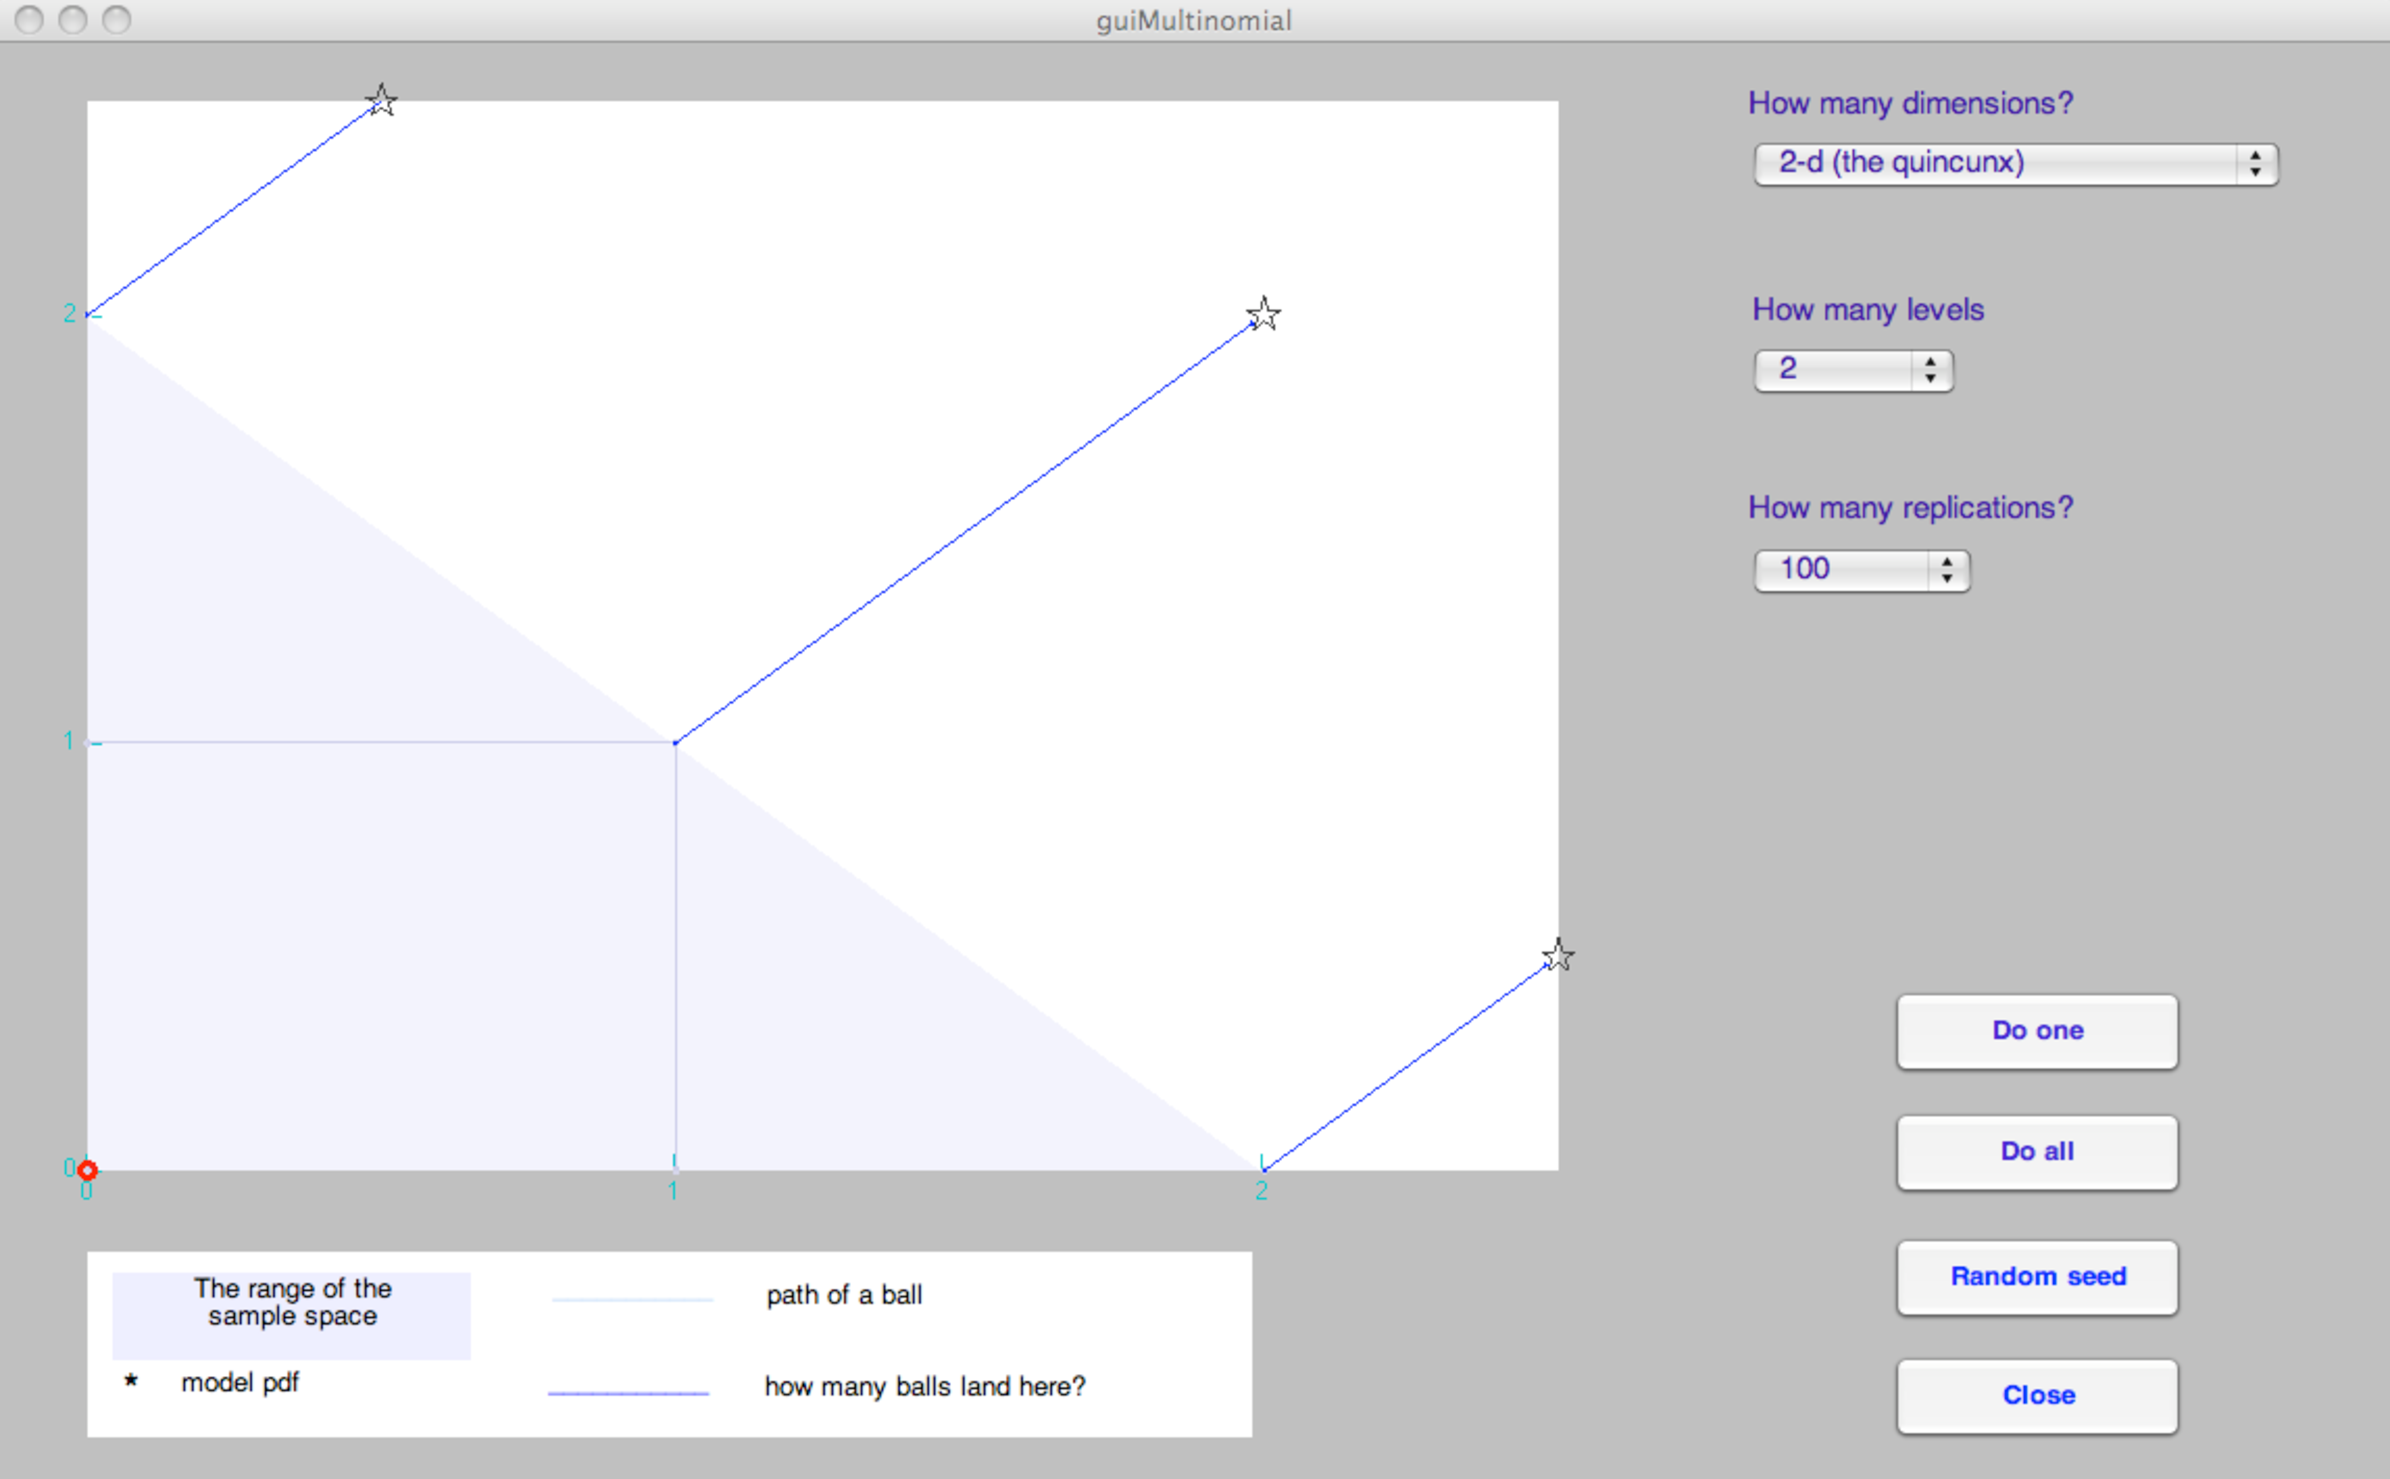
\includegraphics[width=3.00in]{figures/guiMultinomialQuincunx}}
\centering   \makebox{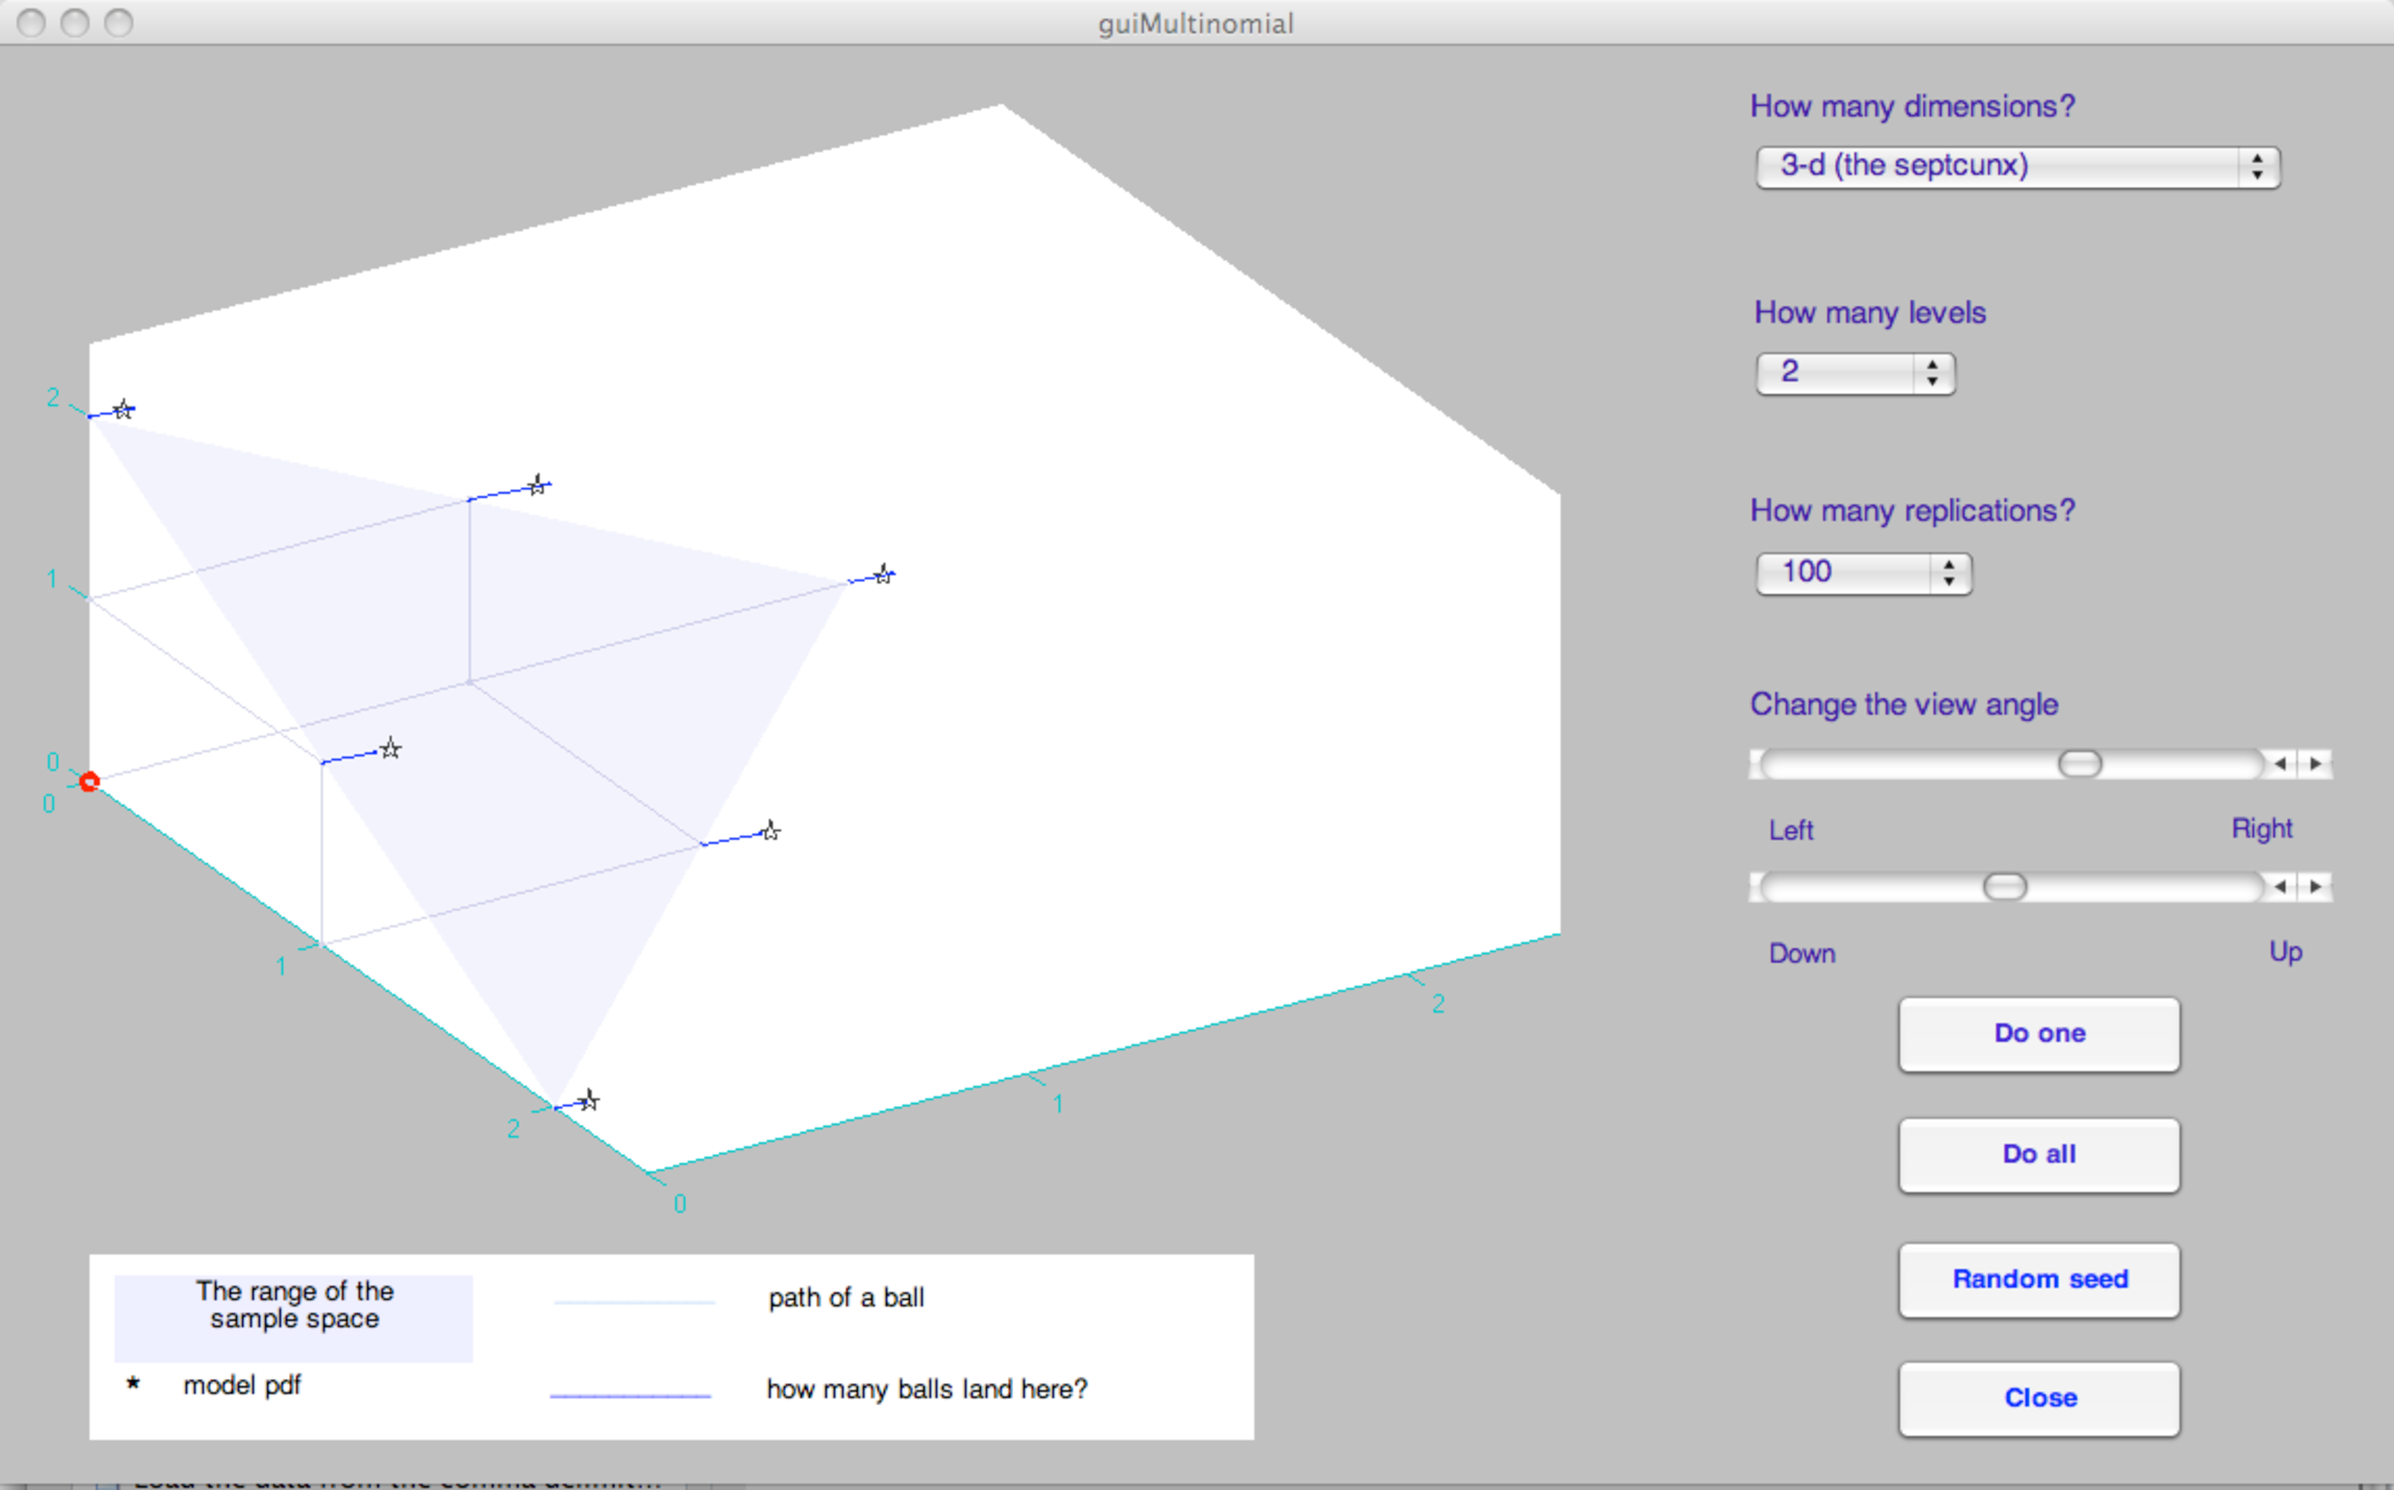
\includegraphics[width=3.00in]{figures/guiMultinomialSeptcunx}}
\end{figure}
%}%end remove

\begin{figure}[htpb]
\caption{Quincunx on the Cartesian plane.  Simulations of $\binomial(n=10,\theta=0.5)$ RV as the x-coordinate of the ordered pair resulting from the culmination of sample trajectories formed by the accumulating sum of $n=10$ IID $\bernoulli(\theta=0.5)$ random vectors over $\{(1,0),(0,1)\}$ with probabilities $\{\theta,1-\theta\}$, respectively.  The blue lines and black asterisks perpendicular to and above the diagonal line, i.e.~the line connecting $(0,10)$ and $(10,0)$, are the density histogram of the samples and the PMF of our $\binomial(n=10,\theta=0.5)$ RV, respectively.\label{F:BinomQuincunxn10r10r1000}}
\centering
\mbox{\subfigure[Ten samples]{\hspace{-2cm} \includegraphics[width=3.250in]{figures/BinomQuincunxn10r10}} \hspace{-2cm}
	   \subfigure[Thousand samples]{\includegraphics[width=3.250in]{figures/BinomQuincunxn10r1000}} }
\end{figure}


We are now ready to extend the $\binomial(n,\theta)$ RV or \rv~to its multivariate version called the $\multinomial(n,\theta_1,\theta_2,\ldots,\theta_k)$ \rv.  We develop this \rv~as the sum of $n$ IID $\demoivre(\theta_1,\theta_2,\ldots,\theta_k)$ \rv~that is defined next by extending $\demoivre(\theta_1,\theta_2,\ldots,\theta_k)$ RV taking values in $\{1,2,\ldots,k\}$ of Model~\ref{M:demoivre} to its vector-valued cousin taking values in $\{e_1, e_2,\ldots,e_k\}$, the ortho-normal basis vectors in $\Rz^k$.

\begin{model}[$\demoivre(\theta_1,\theta_2,\ldots,\theta_k)$ \rv]\label{M:deMoivreRVec}
The PMF of the $\demoivre(\theta_1,\theta_2,\ldots,\theta_k)$ \rv~$X := (X_1,X_2,\ldots,X_k)$ taking value $x := (x_1,x_2,\ldots,x_k) \in \{e_1,e_2,\ldots,e_k\}$, where the $e_i$'s are ortho-normal basis vectors in $\Rz^k$ is:
\[
f(x;\theta_1,\theta_2,\ldots,\theta_k) := P(X=x) = \sum_{i=1}^k \theta_i \BB{1}_{\{e_i\}}(x) =
\begin{cases}
\theta_1 & \text{if} \quad x=e_1:=(1,0,\ldots,0) \in \Rz^k \\
\theta_2 & \text{if} \quad x=e_2:=(0,1,\ldots,0) \in  \Rz^k \\
\vdots \\
\theta_k & \text{if} \quad x=e_k:=(0,0,\ldots,1) \in  \Rz^k \\
0 & \text{otherwise}
\end{cases}
\]
Of course, $\sum_{i=1}^k \theta_i = 1$.
\end{model}

When we add $n$ IID $\demoivre(\theta_1,\theta_2,\ldots,\theta_k)$ \rv~together, we get the $\multinomial(n,\theta_1,\theta_2,\ldots,\theta_k)$ \rv~as defined below.

\begin{model}[$\multinomial(n,\theta_1,\theta_2,\ldots,\theta_k)$ \rv]\label{M:Multinomial}
We say that a \rv~$Y:=(Y_1,Y_2,\ldots,Y_k)$ obtained from the sum of $n$ IID $\demoivre(\theta_1,\theta_2,\ldots,\theta_k)$ \rv{s} with realizations
$$y:=(y_1,y_2,\ldots,y_k) \in \Yz:= \{(y_1,y_2,\ldots,y_k) \in \Zz_+^k : \sum_{i=1}^k y_i = n\}$$ has the PMF given by:
\[
f(y;n,\theta) := f(y;n,\theta_1,\theta_2,\ldots,\theta_k) := P(Y=y;n,\theta_1,\theta_2,\ldots,\theta_k) = \binom{n}{y_1,y_2,\ldots,y_k} \prod_{i=1}^k \theta_i^{y_i} \ ,
\]
where, the multinomial coefficient:
\[
 \binom{n}{y_1,y_2,\ldots,y_k} := \frac{n!}{y_1! y_2! \cdots y_k!} \ .
\]
Note that the marginal PMF of $Y_j$ is $\binomial(n,\theta_j)$ for any $j=1,2,\ldots,k$.
\end{model}

We can visualize the $\multinomial(n,\theta_1,\theta_2,\theta_3)$ process as a sum of $n$ IID $\demoivre(\theta_1,\theta_2,\theta_3)$ \rv{s} via a three dimensional extension of the Quincunx called the ``Septcunx'' and relate the number of paths that lead to a given trivariate sum $(y_1,y_2,y_3)$ with $\sum_{i=1}^3 y_i = n$ as the multinomial coefficient $\frac{n!}{y_1! y_2! y_3!}$.  In the Septcunx, balls choose from one of three paths along $e_1$, $e_2$ and $e_3$ with probabilities $\theta_1$, $\theta_2$ and $\theta_3$, respectively, in an IID manner at each of the $n$ levels, before they collect at buckets placed at the integral points in the $3$-simplex, $\Yz = \{(y_1,y_2,y_3) \in \Zz_+^3 : \sum_{i=1}^3 y_i=n \}$.  Once again, we can visualize that the sum of $n$ IID $\demoivre(\theta_1,\theta_2,\theta_3)$ \rv{s} constitute the $\multinomial(n,\theta_1,\theta_2,\theta_3)$ \rv.%~as depicted in \hyperref[F:MultinomSeptcunxn2n10r1000]{Figure \ref*{F:MultinomSeptcunxn2n10r1000}}.

\begin{labwork}[Septcunx Sampler Demo -- Sum of n IID $\demoivre(1/3,1/3,1/3)$ \rv{s}]\label{LW:SeptcunxSampler}
{\rm
Let us understand the Septcunx construction of the $\multinomial(n,1/3,1/3,1/3)$ \rv $X$ as the sum of $n$ independent and identical $\demoivre(1/3,1/3,13/)$ \rv{s} by calling the interactive visual cognitive tool as follows:
\begin{VrbM}
>> guiMultinomial
\end{VrbM}
}
\end{labwork}

Multinomial distributions are at the very foundations of various machine learning algorithms, including, filtering junk email, learning from large knowledge-based resources like www, Wikipedia, word-net, etc.


\begin{model}[$\normal(\mu,\Sigma)$ \rv]\label{M:MultivariateNormal}
The univariate $\normal(\mu,\sigma^2)$ RV has two parameters, $\mu \in \Rz$ and $\sigma^2 \in (0,\infty)$.  
In the multivariate version $\mu \in \Rz^{m \times 1}$ is a column vector and $\sigma^2$ is replaced by a matrix $\Sigma$.  To begin, let
\[
Z = 
\left( 
\begin{array}{c}
Z_1 \\
Z_2 \\
\vdots \\
Z_m 
\end{array} 
\right)
\]
where, $Z_1,Z_2,\ldots,Z_m$ are jointly independent $\normal(0,1)$ RVs.  Then the JPDF of $Z$ is
\[
f_Z(z) = f_{Z_1,Z_2,\ldots,Z_m}(z_1,z_2,\ldots,z_m) = \frac{1}{(2 \pi)^{m/2}} \exp \left( -\frac{1}{2} \sum_{j=1}^m z_j^2 \right) = \frac{1}{(2 \pi)^{m/2}} \exp \left( -\frac{1}{2} z^T z \right)
\]
We say that $Z$ has a standard multivariate normal distribution and write $Z \sim \normal(0,I)$, where it is understood that $0$ represents the vector of $m$ zeros and $I$ is the $m \times m$ identity matrix (with $1$ along the diagonal entries and $0$ on all off-diagonal entries).

More generally, a vector $X$ has a multivariate normal distribution denoted by $X \sim \normal(\mu,\Sigma)$, if it has joint probability density function
\[
f_X(x;\mu,\Sigma) = f_{X_1,X_2,\ldots,X_m}(x_1,x_2,\ldots,x_m; \mu,\Sigma) 
= \frac{1}{(2 \pi)^{m/2} |(\Sigma)|^{1/2}} \exp \left( -\frac{1}{2} (x - \mu)^T \Sigma^{-1} (x - \mu )\right) 
\]
where $|\Sigma|$ denotes the determinant of $\Sigma$, $\mu$ is a vector of length $m$ and $\Sigma$ is a $m \times m$ symmetric, positive definite matrix.  Setting $\mu=0$ and $\Sigma=I$ gives back the standard multivariate normal \rv.
\end{model}



%bivariate Normal

\begin{figure}[htpb]
\caption{JPDF, Marginal PDFs and Frequency Histogram of Bivariate Standard Normal \rv.\label{F:BivariateStdNormalJPDFMPDFsFreHist}}
\centering   \makebox{\includegraphics[width=6.50in]{figures/BivariateStdNormalJPDFMPDFsFreHist.eps}}
\end{figure}

When we have a non-zero mean vector 
$$\mu=\begin{pmatrix} \mu_X\\ \mu_Y \end{pmatrix} =\begin{pmatrix} 6.49\\ 5.07 \end{pmatrix}$$ 
for the mean lengths and girths of cylindrical shafts from a manufacturing process with  
variance-covariance matrix 
$$\Sigma = \begin{pmatrix} \cv(X,X) & \cv(X,Y)\\ \cv(Y,X) & \cv(Y,Y)\end{pmatrix} = \begin{pmatrix} V(X) & \cv(X,Y)\\ \cv(X,Y) & V(Y)\end{pmatrix} = \begin{pmatrix} 0.59 & 0.24\\ 0.24 & 0.26 \end{pmatrix}$$
then the $\normal(\mu,\Sigma)$ \rv~has JPDF, marginal PDFs and samples with frequency histograms as shown in Figure~\ref{F:BivariateShaftsNormalJPDFMPDFsFreHist}.

We can use \Matlab to compute for instance the probability that a cylinder has length and girth below $6.0$ cms as follows:
\begin{VrbM}
>> mvncdf([6.0 6.0],[6.49 5.07],[0.59  0.24; 0.24 0.26])
ans =    0.2615
\end{VrbM}
Or find the probability (with numerical error tolerance) that the cylinders are within the rectangular specifications of $6\pm1.0$ along $x$ and $y$ as follows:
\begin{VrbM}
>> [F err] = mvncdf([5.0 5.0], [7.0 7.0], [6.49 5.07],[0.59  0.24; 0.24 0.26])

F =    0.3352

err =   1.0000e-08
\end{VrbM}


\begin{figure}[htpb]
\caption{JPDF, Marginal PDFs and Frequency Histogram of a Bivariate Normal \rv~for lengths of girths of cylindrical shafts in a manufacturing process (in cm).\label{F:BivariateShaftsNormalJPDFMPDFsFreHist}}
\centering   \makebox{\includegraphics[width=6.50in]{figures/BivariateShaftsNormalJPDFMPDFsFreHist.eps}}
\end{figure}

\remove{
\iftoggle{PlaceTutsHere}{%
\subsection{Tutorial Exercises}
\input{Tutorials/Tut_RandVecs_preps.tex}
~\\
\input{Tutorials/Tut_RandVecs_inTut.tex}
}{%
  % don't do anything otherwise
}

}%remove


\subsection{Dependent Random Variables}
When a sequence of RVs are not independent they are said to be {\bf dependent}.  
The simplest form of dependence is {\em Markov dependence} that we will briefly see via a couple examples in Chapter~\ref{C:FiniteMarkovChains}.

\section{Exercises in Multivariate Random Variables}\label{S:xsMultivariateRVs}
\begin{ExerciseList}
%question 9 (cts )
\Exercise
Find the probability that none of the three bulbs in a traffic signal, that are assumed to have independent life-times (i.e., the time during which they are operational), need to be replaced during the first 1200 hours of operation if the length of time before a single bulb needs to  be replaced is a continuous random variable $X$ with density
$$f(x)\;=\;\begin{cases}6\left(0.25-(x-1.5)^2\right)&1<x<2\\0&\textrm{otherwise}\end{cases}\enspace.$$
Note: $X$ is measured in multiples of 1000 hours.
\Answer
The probability that  \emph{one}  light bulb doesn't need to be replaced in  1200 hours is:
\ba{\p(X>1.2)&\;=\;1-\p(X<1.2)\\[3pt]
&=\;1\;-\;\int^{1.2}_1 6 (0.25-(x-1.5)^2)\,dx\\[3pt]
&=\;1\;-\;\int^{1.2}_1 6(0.25-x^2+3x-2.25)\,dx\\[3pt]
&=\;1\;-\;\int^{1.2}_1 (-6x^2+18x-12)\,dx\\[3pt]
&=\;1\;-\;\left[-2x^3+9x^2-12x\right]^{1.2}_1\\[3pt]
&=\;1-0.1040\\[3pt]
&\;=\;0.8960}
Assuming  that   the three light bulbs function  independently of  each
other, the probability that none of them need to be replaced in the
first 1200 hours is
$$\p(\{X_1>1.2\}\cap\{X_2>1.2\}\cap\{X_3>1.2\}\;=\;0.8960^3\;=\;
0.7193$$
where $X_i$ is the length of time that bulb $i$ lasts.

\Exercise
Let $(X,Y)$ be a continuous \rv~with joint probability density function (JPDF)
\[
f_{X,Y}(x,y)
=
\begin{cases}
a (x^2+y) & \text{ if } 0 < x < 1 \text{ and } 0 < y < 1\\
0 & \text{ otherwise} \enspace .
\end{cases}
\]
Find the following:
\be
\item~the normalizing constant $a$ which will ensure $\p(\Omega) = \int_{-\infty}^{\infty}\int_{-\infty}^{\infty} f_{X,Y}(x,y) dx dy = 1$
\item~$f_X(x) = \int_{-\infty}^{\infty} f_{X,Y}(x,y) dy$ called the marginal probability density function (MPDF) of $X$
\item~$f_Y(y) = \int_{-\infty}^{\infty} f_{X,Y}(x,y) dx$ called the marginal probability density function (MPDF) of $Y$
\item Check if $f_X(x)f_Y(y)=f_{X,Y}(x,y)$ for every $(x,y)$ and decide whether $X$ and $Y$ are independent random variables.  {Hint: $X$ and $Y$ are said to be independent if $f_X(x)f_Y(y)=f_{X,Y}(x,y)$ for every $(x,y)$.}
\item~$F_{X,Y}(x,y)$, the joint cumulative distribution function (JCDF) of $(X,Y)$ for any $(x,y) \in (0,1) \times (0,1)$ 
\item~the probability that $X > 0.5$ and $Y<0.6$, i.e., $\p(X>0.5,Y<0.6)$
\item~$E(X)$, the expectation of $X$ or the first moment of $X$
\item~$E(Y)$, the expectation of $Y$ or the first moment of $Y$
\item~$E(XY)$, the expectation of $XY$
\item~$\cv(X,Y)=E(XY)-E(X)E(Y)$, the covariance of $X$ and $Y$.
\ee

\Answer
~\\
\be
\item~To find $a$ we simply set $1=\int_{-\infty}^{\infty}\int_{-\infty}^{\infty} f_{X,Y}(x,y) dx dy$ and solve for $a$ as follows:
\begin{align*}
1
&=
\int_{-\infty}^{\infty}\int_{-\infty}^{\infty} f_{X,Y}(x,y) dx dy = \int_{0}^{1}\int_{0}^{1} a(x^2+y) dx dy\\
&=
a\int_{0}^{1}\int_{0}^{1} (x^2+y) dx dy = a\int_{0}^{1} \left[ \frac{1}{3}x^3+yx \right]_{x=0^1} dy\\
&=
a\int_{0}^{1} \left( \frac{1}{3}+y - 0 \right) dy = a \left[ \frac{y}{3}+\frac{1}{2}y^2 \right]_{y=0}^{1}\\
&=
a \left( 0-\left(\frac{1}{3}+\frac{1}{2}1^2\right) \right) = a \left( \frac{1}{3}+\frac{1}{2} \right)\\
&=
a \left( \frac{5}{6} \right)
\end{align*}
Therefore $a=6/5$ and the joint PDF is
\[
f_{X,Y}(x,y)
=
\begin{cases}
\frac{6}{5} (x^2+y) & \text{ if } 0 < x < 1 \text{ and } 0 < y < 1\\
0 & \text{ otherwise} \enspace .
\end{cases}
\]
\item~First compute the marginal PDF $f_X(x)$ for any $x \in (0,1)$ by integrating over $y$
\begin{align*}
f_X(x) 
&= \int_{-\infty}^{\infty} f_{X,Y}(x,y) dy
= \int_0^1 \frac{6}{5} (x^2+y) dy 
= \left[ \frac{6}{5} (yx^2+y^2/2) \right]_{y=0}^1\\
&= \frac{6}{5} \left((1 \times x^2 + 1^2/2) - 0 \right)
= \frac{6}{5} \left( x^2 + \frac{1}{2} \right)
\end{align*}
Finally, the marginal PDF of the RV $X$ in the first component of the \rv~$(X,Y)$ is
\[
f_{X}(x)
=
\begin{cases}
\frac{6}{5} \left( x^2 + \frac{1}{2} \right) & \text{ if } 0 < x < 1\\
0 & \text{ otherwise} \enspace .
\end{cases}
\]
\item~Similarly, the marginal PDF $f_Y(y)$ for any $y \in (0,1)$ by integrating over $x$ is 
\[
f_Y(y)=\int_{-\infty}^{\infty} f_{X,Y}(x,y) dx = \int_0^1 \frac{6}{5}(x^2+y) dx = \frac{6}{5} \left[ x^3/3+yx\right]_{x=0}^1 = \frac{6}{5}(y+1/3).
\]
Finally, the marginal PDF of the RV $Y$ in the second component of the \rv~$(X,Y)$ is
\[
f_{Y}(y)
=
\begin{cases}
\frac{6}{5} \left( y + \frac{1}{3} \right) & \text{ if } 0 < y < 1\\
0 & \text{ otherwise} \enspace .
\end{cases}
\]
\item The product of marginal PDFs of $X$ and $Y$ does not equal the joint PDF of $(X,Y)$ for values of $(x,y) \in (0,1)^2$
\[
f_X(x)f_Y(y) = \frac{6}{5} \frac{6}{5} \left( y + \frac{1}{3} \right) \left( x^2 + \frac{1}{2} \right) = \frac{6}{25} \left( 6 x^2y+2x^2+3y+1\right) \neq \frac{6}{5}(x^2+y) = f_{X,Y}(x,y)
\]
Therefore $X$ and $Y$ are not independent random variables (they are dependent!).
\item~The joint distribution function $F_{X,Y}(x,y)$ for any $(x,y) \in (0,1)^2$ is
\begin{align*}
F_{X,Y}(x,y) 
&= \int_{-\infty}^{y} \int_{-\infty}^{x} f_{X,Y}(u,v) du dv
= \int_{0}^{y} \int_{0}^{x} \frac{6}{5} (u^2+v) du dv
= \frac{6}{5} \int_{0}^{y} \left[ \frac{u^3}{3}+vu) \right]_{u=0}^{x} dv\\
&= \frac{6}{5} \int_{0}^{y} \left( \frac{x^3}{3}+vx - 0 \right) dv
= \frac{6}{5} \left[ \frac{x^3v}{3}+\frac{v^2x}{2} \right]_{v=0}^{y}
= \frac{6}{5} \left( \frac{x^3y}{3}+\frac{y^2x}{2} - 0 \right)\\
&= \frac{6}{5} \left( \frac{x^3y}{3}+\frac{y^2x}{2} - 0 \right)
\end{align*}
\item~
\begin{align*}
\p(X>0.5,Y<0.6) 
&= \int_{-\infty}^{0.6} \int_{0.5}^{\infty} f_{X,Y}(x,y) dx dy
= \int_{0}^{0.6} \int_{0.5}^{1} \frac{6}{5} (x^2+y) dx dy\\
&= \frac{6}{5} \int_{0}^{0.6} \left[ \frac{x^3}{3}+yx \right]_{x=0.5}^{1} dy
= \frac{6}{5} \int_{0}^{0.6} \left(\frac{7}{24} + \frac{y}{2} \right) dy\\
&= \frac{6}{5} \left[\frac{7}{24}y + \frac{y^2}{2} \right]_{y=0}^{0.6}
= \frac{6}{5} \left(\frac{7}{24}\times \frac{6}{10} + \frac{36}{400} \right)
=0.318
\end{align*}
\item~
\begin{align*}
E(X) 
&= \int_{-\infty}^{\infty} \int_{-\infty}^{\infty} x f_{X,Y}(x,y) dx dy\\
&=\frac{6}{5} \int_{0}^{1} \int_{0}^{1}  x \left( x^2 + y \right) dx dy
=\frac{6}{5} \int_{0}^{1} \int_{0}^{1}  \left( x^3 + xy \right) dx dy
= \frac{6}{5} \int_{0}^{1} \left[ \frac{x^4}{4} + \frac{1}{2}x^2y\right]_{x=0}^{1} dy\\
&=\frac{6}{5} \int_{0}^{1} \left( \frac{1}{4} + \frac{y}{2} - 0 - 0\right) dy
= \frac{6}{5} \left[ \frac{y}{4} + \frac{y^2}{4} \right]_{y=0}^{1} 
= \frac{6}{5} \left(\frac{1}{4} + \frac{1}{4} - 0 - 0 \right) = \frac{6}{5}\times \frac{1}{2}=\frac{3}{5}
\end{align*}
\item~
\begin{align*}
E(Y) 
&= \int_{-\infty}^{\infty} \int_{-\infty}^{\infty} y f_{X,Y}(x,y) dx dy\\
&= \int_{0}^{1} \int_{0}^{1} y \frac{6}{5} \left( x^2 + y \right) dx dy
= \frac{6}{5} \int_{0}^{1} \int_{0}^{1}  \left( x^2y + y^2 \right) dx dy
= \frac{6}{5} \int_{0}^{1} \left[ \frac{x^3y}{3} + y^2x \right]_{x=0}^{1} dy\\
&= \frac{6}{5} \int_{0}^{1} \left( \frac{y}{3} + y^2 -0-0\right) dy
= \frac{6}{5} \left[ \frac{y^2}{6} + \frac{y^3}{3} \right]_{y=0}^{1} 
= \frac{6}{5} \left( \frac{1}{6} + \frac{1}{3} + - 0 -0 \right) = \frac{6}{5} \times \frac{3}{6}=\frac{3}{5}
\end{align*}
\item~
\begin{align*}
E(XY) 
&= \int_{-\infty}^{\infty} \int_{-\infty}^{\infty} xy f_{X,Y}(x,y) dx dy\\
&=\frac{6}{5} \int_{0}^{1} \int_{0}^{1}  xy \left( x^2 + y \right) dx dy
=\frac{6}{5} \int_{0}^{1} \int_{0}^{1} x^3y+xy^2 dx dy
=\frac{6}{5} \int_{0}^{1} \left[ \frac{x^4}{4}y+\frac{x^2 y^2}{2} \right]_{x=0}^1 dy\\
&=\frac{6}{5} \int_{0}^{1} \left( \frac{y}{4} + \frac{y^2}{2} -0-0\right)dy
=\frac{6}{5} \left[ \frac{y^2}{8} + \frac{y^3}{6}\right]_{y=0}^1 
=\frac{6}{5} \left(\frac{1}{8} + \frac{1}{6}-0-0\right)\\
&=\frac{6}{5} \left(\frac{3}{24}+\frac{4}{24}\right)=\frac{6}{5}\times\frac{7}{24}=\frac{7}{20}
\end{align*}
\item~
\[
\cv(X,Y) = E(XY)-E(X)E(Y) = \frac{7}{20}-\left(\frac{3}{5} \times \frac{3}{5} \right) = \frac{7}{20}-\frac{9}{25} = \frac{35}{100}-\frac{36}{100} = -\frac{1}{100}
\]
\ee

\Exercise
Logs are milled to have a width of $\mu$.
The actual width of a randomly selected item is $X$.
If $X$ is a $\normal(\mu,\sigma^2)$ random variable then find the probability density function of the {\em squared-error} of the milling process,
\[ Y\,=\, (X-\mu)^2\,.\]
\Answer
Note that $Y= (X-\mu)^2$ is not on-to-one so it is better to use the direct method by differentiating the distribution function  of $Y$, $F_Y(y)$,  to obtain $f_Y(y)$.

If $y\geqslant 0$,
\begin{align*}
 F_Y(y)\;=&\; \p(Y \leqslant y) \\[3pt]
 \;=&\;  \p( (X-\mu)^2 \leqslant y) \\[3pt]
 \;=&\; \p(-\sqrt y \leqslant X-\mu \leqslant \sqrt y)\\[3pt]
 \;=&\; \p(\mu -\sqrt y \leqslant X  \leqslant \mu + \sqrt y)\\[3pt]
\;=&\; F_X( \mu + \sqrt y) \,-\, F_X( \mu + \sqrt y)
\end{align*}

Differentiating this expression gives
\begin{align*}
f_Y(y) \;=&\; \frac{d}{dy} \left(F_X( \mu + \sqrt y) \,-\, F_X( \mu - \sqrt y)  \right) \\[3pt]
\;=&\;\frac{1}{2} y^{-\frac{1}{2}} \, f_X (\mu + \sqrt y ) \,- \, \left( -\frac{1}{2} y^{-\frac{1}{2}} \right)\, f_X (\mu - \sqrt y ) \\[3pt]
\;=&\;\frac{1}{2 \sqrt y } \left(  f_X (\mu + \sqrt y )  + f_X (\mu - \sqrt y )  \right)
\end{align*}

Note: If $y<0$ then $f_Y(y) = 0$  since  $F_Y(y)=0$ in this case.

\Exercise
Let $(X,Y)$ be a discrete random vector (\rv) with support:
\[
\mathcal{S}_{X,Y} = \{(0,0),(0,1),(1,0),(1,1)\} \enspace .
\]
Let its joint probability mass function (JPMF) be:
\[
f_{X,Y}(x,y) = 
\begin{cases}
\frac{1}{4} & \text{ if } (x,y)=(0,0)\\
\frac{1}{4} & \text{ if } (x,y)=(0,1)\\
\frac{1}{4} & \text{ if } (x,y)=(1,0)\\
\frac{1}{4} & \text{ if } (x,y)=(1,1)\\
0 & \text{ otherwise} \enspace .
\end{cases}
\]
Are $X$ and $Y$ independent? 
\Answer
~\\
First derive the marginal PMF of $X$ and $Y$ and then check if the JPMF is the product of the marginal PMFs.
\[
f_X(0) = \sum_{y \in \mathcal{S}_{X,Y}} f_{X,Y}(0,y) = f_{X,Y}(0,0) + f_{X,Y}(0,1) = \frac{1}{4}+\frac{1}{4}=\frac{1}{2}
\]
and
\[
f_X(1) = \sum_{y \in \mathcal{S}_{X,Y}} f_{X,Y}(1,y) = f_{X,Y}(1,0) + f_{X,Y}(1,1) = \frac{1}{4}+\frac{1}{4}=\frac{1}{2}
\]
Thus,
\[
f_{X}(x) = 
\begin{cases}
\frac{1}{2} & \text{ if } x = 0\\
\frac{1}{2} & \text{ if } x = 1\\
0 & \text{ otherwise} \enspace .
\end{cases}
\]
Similarly,
\[
f_{Y}(y) = 
\begin{cases}
\sum_{x \in \mathcal{S}_{X,Y}} f_{X,Y}(x,0)=f_{X,Y}(0,0) + f_{X,Y}(1,0) = \frac{1}{4}+\frac{1}{4}=\frac{1}{2} & \text{ if } y = 0\\
\sum_{x \in \mathcal{S}_{X,Y}} f_{X,Y}(x,1)=f_{X,Y}(0,1) + f_{X,Y}(1,1) = \frac{1}{4}+\frac{1}{4}=\frac{1}{2} & \text{ if } y = 1\\
0 & \text{ otherwise} \enspace .
\end{cases}
\]
Finally, the product of $f_X(x)$ and $f_Y(y)$ is
\[
f_{X}(x) \times f_{Y}(y) = 
\begin{cases}
\frac{1}{2} \times \frac{1}{2}=\frac{1}{4} & \text{ if } (x,y)=(0,0)\\
\frac{1}{2} \times \frac{1}{2}=\frac{1}{4} & \text{ if } (x,y)=(0,1)\\
\frac{1}{2} \times \frac{1}{2}=\frac{1}{4} & \text{ if } (x,y)=(1,0)\\
\frac{1}{2} \times \frac{1}{2}=\frac{1}{4} & \text{ if } (x,y)=(1,1)\\
0 & \text{ otherwise} \enspace .
\end{cases}
\]
which in turn is equal to the JPMF $f_{X,Y}(x,y)$ in the question.  Therefore we have shown that the component RVs $X$ and $Y$ in the \rv~$(X,Y)$ are indeed indepedent.

\Exercise
A semiconductor product consists of three layers that are fabricated independently.  
If the variances in thickness of the first, second and third third layers are $25$, $40$ and $30$ nanometers squared, what is the variance of the thickness of the final product? 
\Answer
~\\
Let $X_1$, $X_2$, $X_3$ be independent RVs that denote the thickness of the first, second and third layer, respectively.  Let $X$ denote the thickness of the final product.  Then
\[
X= X_1+X_2+X_3
\]
By the property that $V\left(\sum_{i=1}^n a_i X_i\right) = \sum_{i=1}^n a_i^2 V(X_i)$, Variance of $X$ is
\[
V(X) = 1^2 V(X_1) + 1^2 V(X_2) + 1^2 V(X_3) = 25+40+30 = 95 nm^2 \enspace .
\] 
This shows how the variance in each layer is propagated to the variance of the final product.

\Exercise
Find the covariance for the discrete \rv~$(X,Y)$ with joint probability mass function
\[
f_{X,Y}(x,y) = 
\begin{cases}
0.2 & \text{ if } (x,y)=(0,0)\\
0.1 & \text{ if } (x,y)=(1,1)\\
0.1 & \text{ if } (x,y)=(1,2)\\
0.1 & \text{ if } (x,y)=(2,1)\\
0.1 & \text{ if } (x,y)=(2,2)\\
0.4 & \text{ if } (x,y)=(3,3)\\
0 & \text{ otherwise } \enspace .
\end{cases}
\]
[Hint: Recall that $\cv(X,Y)=E(XY)-E(X)E(Y)$]
\Answer
~\\
Find $E(XY)$, $E(X)$ and $E(Y)$ to get $\cv(X,Y)=E(XY)-E(X)E(Y)$ as follows:
\begin{multline*}
E(XY) = \sum_{(x,y) \in \mathcal{S}_{X,Y}} x \times y \times f_{X,Y}(x,y) \\
= 0 \times 0 \times 0.2 + 1 \times 1 \times 0.1+ 1 \times 2 \times 0.1 + 2 \times 1 \times 0.1 + 2 \times 2 \times 0.1 + 3 \times 3 \times 0.4 = 4.5
\end{multline*}
\begin{multline*}
E((X,Y)) = \sum_{(x,y) \in \mathcal{S}_{X,Y}} (x , y) \times f_{X,Y}(x,y) \\
= (0 , 0) \times 0.2 + (1 , 1) \times 0.1 + (1 , 2) \times 0.1 + (2 , 1) \times 0.1 + (2 , 2) \times 0.1 + (3 , 3) \times 0.4\\= (0,0)+(0.1,0.1)+(0.1,0.2)+(0.2,0.1)+(0.2,0.2)+(1.2,1.2) \\
= (1.8,1.8) 
\end{multline*}
Since addition is component-wise $E((X,Y))=(E(X),E(Y))$ and therefore $E(X)=E(Y)=1.8$.

Alternatively, you can first find the marginal PMFs $f_X$ and $f_Y$ for $X$ and $Y$ and then take the expectations $E(X)=\sum_x x \times f_X(x)$ and $E(Y)=\sum_y y \times f_Y(y)$.

Finally, 
\[
\cv(X,Y) = E(XY)-E(X)E(Y) = 4.5 - 1.8^2 = 1.26 \enspace .
\]

\Exercise
Consider two random variables (RVs) $X$ and $Y$ having marginal distribution functions
\[
F_X(x) =
\begin{cases}
0 & \text{ if } x < 1\\
\frac{1}{2} & \text{ if } 1 \leq x < 2\\
1 & \text{ if } x \geq 2\\
\end{cases}
\] 
\[
F_Y(y) =
\begin{cases}
0 & \text{ if } y < 0\\
1-\frac{1}{2}e^{-y}-\frac{1}{2}e^{-2y} & \text{ if } y \geq 0\\
\end{cases}
\]
If $X$ and $Y$ are independent, what is their joint distribution function $F_{X,Y}(x,y)$? [Hint: you need to express $F_{X,Y}(x,y)$ for any $(x,y) \in \Rz^2$.]
\Answer
~\\
Since $X$ and $Y$ are independent, $F_{X,Y}(x,y) = F_X(x) F_Y(y)$ for all $(x,y) \in \Rz^2$, and we get:
\[
F_{X,Y}(x,y) = 
\begin{cases}
0 & \text{ if } x < 1 \text{ or } y < 0\\
\frac{1}{2}\left(1-\frac{1}{2}e^{-y}-\frac{1}{2}e^{-2y}\right) & \text{ if } 1 \leq x < 2 \text{ and } y \geq 0\\
1-\frac{1}{2}e^{-y}-\frac{1}{2}e^{-2y} & \text{ if } x \geq 2 \text{ and } y \geq 0
\end{cases}
\]
{\small
You can arrive at the answer by partitioning $x$-axis into $(-\infty,1)$, $[1,2)$ and $[2,\infty)$ where $F_X(x)$ takes distinct values.  Similarly, partition the $y$-axis into  $(-\infty,0)$ and $[0,\infty)$ where $F_Y(y)$ takes distinct values.  
Now $(x,y)$ can take values in one of these $3 \times 2=6$ partitions of the $x \times y$ plane as follows (make a picture!):
\[
(-\infty,1) \times (-\infty,0), \,
[1,2) \times (-\infty,0), \,
[2,\infty) \times (-\infty,0), \,
(-\infty,1) \times [0,\infty), \,
[1,2) \times [0,\infty), \,
[2,\infty) \times [0,\infty) \enspace .
\]
Now work out what $F_{X,Y}(x,y) = F_X(x) F_Y(y)$ is for $(x,y)$ in each of the above six partitions of the plane and you will get the the expression for $F_{X,Y}(x,y)$ given above.
}

\Exercise
Let $(X,Y)$ be a continuous \rv~with joint probability density function (JPDF):
\[
f_{X,Y}(x,y) = 
\begin{cases}
e^{-x} & \text{ if } x \in [0,\infty) \text{ and }  y \in [2,3]\\
0 & \text{otherwise} \enspace .
\end{cases}
\]
Are $X$ and $Y$ independent?
\Answer
~\\
First obtain marginal PDF of $Y$.  If $y \in [2,3]$ then
\[
f_Y(y) = \int_{-\infty}^{\infty} f_{X,Y}(x,y) dx = \int_0^{\infty} e^{-x} dx = \left[ -e^{-x} \right]_0^{\infty} = 0 - (-1)=1 \enspace .
\]
Therefore,
\[
f_Y(y) =
\begin{cases}
1 & \text{ if } y \in [2,3]\\
0 & \text{otherwise} \enspace .
\end{cases}
\]
Now, obtain the marginal PDF of $X$.  If $x \in [0,\infty)$ then
\[
f_X(x) = \int_{-\infty}^{\infty} f_{X,Y}(x,y) dy = \int_2^3 e^{-x} dy  = e^{-x} \int_2^3 1 dy = e^{-x} \left[ y \right]_2^3 = e^{-x} (3-2) = e^{-x} \enspace .
\]
Therefore,
\[
f_X(x) =
\begin{cases}
e^{-x} & \text{ if } x \in [0,\infty)\\
0 & \text{otherwise} \enspace .
\end{cases}
\]
Finally, verifying that $f_{X,Y}(x,y) = f_X(x) f_Y(y)$ for any $(x,y) \in \Rz^2$ is done case by case.  
Draw a picture on the plane to work out the cases from the distinct expressions taken by $f_{X,Y}(x,y)$.  
There are only two cases to consider (when $f_{X,Y}(x,y)$ takes zero values and when $f_{X,Y}(x,y)$ takes non-zero values):
\be
\item~If $x \notin [0,\infty)$ or $y \notin [2,3]$ then $f_X(x)f_Y(y)=0=f_{X,Y}(x,y)$
\item~If $x \in [0,\infty)$ and $y \in [2,3]$ then $f_X(x)f_Y(y)=e^{-x} \times 1=e^{-x}=f_{X,Y}(x,y)$.
\ee
Thus, $X$ and $Y$ are independent.

\Exercise
In an electronic assembly, let the RVs $X_1,X_2,X_3,X_4$ denote the lifetimes of four components in hours.  
Suppose that the JPDF of these variables is
\begin{align*}
~& f_{X_1,X_2,X_3,X_4}(x_1,x_2,x_3,x_4) \\
&\qquad= 
\begin{cases}
9 \times 10^{-12} e^{-0.001 x_1 - 0.002 x_2 - 0.0015 x_3 - 0.003 x_4} & \text{ if } x_1 \geq 0, x_2 \geq 0, x_3 \geq 0, x_4 \geq 0\\
0 & \text{ otherwise} \enspace.
\end{cases}
\end{align*}
What is the probability that the device operates for more than 1000 hours without any failures? [Hint: The requested probability is $\p(X_1>1000,X_2>1000,X_3>1000,X_4>1000)$ since each one of the four components of the device must not fail before 1000 hours.]
\Answer
~\\
\begin{multline*}
\p(X_1>1000,X_2>1000,X_3>1000,X_4>1000) \\
= \int_{1000}^{\infty} \int_{1000}^{\infty} \int_{1000}^{\infty} \int_{1000}^{\infty} 9 \times 10^{-12} e^{-0.001 x_1 - 0.002 x_2 - 0.0015 x_3 - 0.003 x_4} dx_1 dx_2 dx_3 dx_4\\
= 9 \times 10^{-12} \int_{1000}^{\infty} \int_{1000}^{\infty} \int_{1000}^{\infty} \int_{1000}^{\infty}  e^{-0.001 x_1} e^{- 0.002 x_2} e^{- 0.0015 x_3} e^{- 0.003 x_4} dx_1 dx_2 dx_3 dx_4\\
=  9 \times 10^{-12} \int_{1000}^{\infty} e^{-0.001 x_1} \int_{1000}^{\infty} e^{- 0.002 x_2} \int_{1000}^{\infty} e^{- 0.0015 x_3} \int_{1000}^{\infty} e^{- 0.003 x_4} dx_4 dx_3 dx_2 dx_1\\
\end{multline*}
Since
\[
\int_{1000}^{\infty} e^{- a x_i} dx_i = \left[ \frac{e^{-a x_i}}{-a} \right]_{1000}^{\infty} = 0 + \frac{e^{-1000\times a}}{a} \enspace ,
\]
the above quadruply iterated integral becomes
\begin{align*}
&~ 9 \times 10^{-12} \times \frac{e^{-1000 \times 0.001}}{0.001} \times \frac{e^{-1000 \times 0.002}}{0.002} 
\times \frac{e^{-1000 \times 0.0015}}{0.0015} \times \frac{e^{-1000 \times 0.003}}{0.003}\\
&= 9 \times 10^{-12} \times \frac{1000}{1} \times \frac{1000}{2} \times \frac{1000}{1.5} \times \frac{1000}{3} \times
e^{-1} \times e^{-2} \times e^{-1.5} \times e^{-3} \\
&= 9 \times 10^{-12} \times \frac{1}{9} \times 10^{12} \times e^{-7.5} = e^{-7.5} \approxeq 0.00055 \enspace .
\end{align*}

\Exercise
Suppose the RVs $Y_1$, $Y_2$ and $Y_3$ represent the thickness in micrometers of a substrate, an active layer, and a coating layer of a chemical product.  
Assume $Y_1$, $Y_2$ and $Y_3$ are $\normal(10000,250^2)$, $\normal(1000,20^2)$ and $\normal(80,4^2)$ RVs, respectively.  
Further suppose that they are independent.  
The required specifications for the thickness of the substrate, active layer and coating layer are $[9500,10500]$, $[950,1050]$ and $[75,85]$, respectively.  
What proportion of chemical products meets all thickness specifications? [Hint: this is just $\p(9500<Y_1<10500,950<Y_2<1050,75<Y_3<85)$]  Which one of the three thicknesses has the least probability of meeting specifications?   
\Answer
~\\
Due to independence of $Y_1$, $Y_2$ and $Y_3$
\begin{multline*}
\p(9500<Y_1<10500,950<Y_2<1050,75<Y_3<85)\\ = \p(9500<Y_1<10500) \p(950<Y_2<1050) \p(75<Y_3<85)
\end{multline*}
After standardizing each Normal RV (subtracting its mean and dividing by its standard deviation) we get
\begin{align*}
&~ \p(9500<Y_1<10500) \p(950<Y_2<1050) \p(75<Y_3<85)\\
&=  P\left(\frac{9500-10000}{250}< Z < \frac{10500-10000}{250} \right) P\left( \frac{950-1000}{20}<Z<\frac{1050-1000}{20}\right)\\
&\qquad \qquad \qquad \qquad \qquad \qquad P\left(\frac{75-80}{4}<Z<\frac{85-80}{4}\right)\\
&= \p(-2.0<Z<2.0) \p(-2.5<Z<2.5) \p(-1.25<Z<1.25) \\
&= (\Phi(2.0)-(1-\Phi(2.0)) \times (\Phi(2.5)-(1-\Phi(2.5)) \times (\Phi(1.25)-(1-\Phi(1.25))\\
&= (2\Phi(2.0)-1) \times (2\Phi(2.5)-1) \times (2\Phi(1.25)-1)\\
&= ((2 \times 0.9772) -1) \times ((2 \times 0.9938) - 1) \times ((2 \times 0.8944)-1) \qquad \text{ using Table for $\Phi(z)$} \\
&= 0.9544 \times 0.9876 \times 0.7888 = 0.7435
\end{align*}
%To follow the fourth-last equality above see Example 8.14(d) from EMTH119. % TODO? 
The values for the distribution function $\Phi(z)$ of the $\normal(0,1)$ RV $Z$ are in the table on page 67. 

The thickness of the coating layer represented by $Y_3$ has the least probability ($0.7888$) of meeting specifications.  Consequently, a priority should be to reduce variability in this part of the process.

\Exercise
Soft drink cans are filled by an automated filling machine.  
Assume the fill volumes of the cans are independent $\normal(12.1,0.01)$ RVs.  
What is the probability that the average volume of ten cans selected from this process is less than $12.01$ fluid ounces?
\Answer
~\\
Let $X_1,X_2,\ldots,X_{10}$ denote the fill volumes of $10$ cans.  The average fill volume is the sample mean
\[
\ol{X}_{10} = \frac{1}{10} \sum_{i=1}^{10} X_i
\]
By property of Expectations and Variances for linear combinations
\[
E(\ol{X}_{10}) = E \left(\frac{1}{10} \sum_{i=1}^{10} X_i \right) = \frac{1}{10}\sum_{i=1}^nE(X_i) = \frac{1}{10}\sum_{i=1}^nE(X_1) = \frac{1}{10} \times 10 \times E(X_1) = E(X_1) = 12.1
\]
Or by directly using the ``formula'' $E(\ol{X}_{10}) = E(X_1)=12.1$ for these $10$ identically distributed RVs.  
Similarly, 
\[
V\left(\ol{X}_{10}\right) = V \left(\frac{1}{10} \sum_{i=1}^{10} X_i \right) = 10 \times \frac{1}{10^2} V(X_1) = \frac{1}{10} \times 0.01 = 0.001 
\]
Or by directly using the ``formula'' $V(\ol{X}_{10}) = V(X_1)/10$ for these $10$ independently and identically distributed RVs.
 
By the special property of Normal RVs -- a linear combination of independent normal RVs is also normal -- we know that 
$\ol{X}_{10}$ is a $\normal(12.1,0.001)$ RV.
Consequetly, the probability of interest is
\begin{align*}
\p(\ol{X}_{10} < 12.01) 
&= P \left( \frac{\ol{X}_{10}-E(\ol{X}_{10})}{\sqrt{0.001}} < \frac{12.01 - E(\ol{X}_{10})}{\sqrt{0.001}} \right) = P\left(Z < \frac{12.01-12.1}{0.0316}\right)\\ 
&\approxeq \p(Z<-2.85) = 1-\p(Z<2.85) = 1-\Phi(2.85) = 1-0.9978=0.0022
\end{align*}

\Exercise
Let $X_1,X_2,X_3,X_4$ be RVs that denote the number of bits received in a digital channel that are classified as {\em excellent}, {\em good}, {\em fair} and {\em poor}, respectively.  
In a transmission of $10$ bits, what is the probability that $6$ of the bits received are {\em excellent}, $2$ are {\em good}, $2$ are {\em fair} and none are {\em poor} under the assumption that the classification of bits are independent events and that the probabilities of each bit being {\em excellent}, {\em good}, {\em fair} and {\em poor} are $0.6$, $0.3$, $0.08$ and $0.02$, respectively. 
[Hint: Think of $\multinomial(n=10,\theta_1=0.6,\theta_2=0.3,\theta_3=0.08,\theta_4=0.02)$ as a model for bit classification in this digital channel.]
\Answer
~\\
Using the $\multinomial(n=10,\theta_1=0.6,\theta_2=0.3,\theta_3=0.08,\theta_4=0.02)$ \rv~as our model
\begin{align*}
&~ P\left( (X_1,X_2,X_3,X_4)=(6,2,2,0); n=10,\theta_1=0.6,\theta_2=0.3,\theta_3=0.08,\theta_4=0.02 \right)\\ 
&= \frac{10!}{6! \times 2! \times 2! \times 0!} \times 0.6^6 \times 0.3^2 \times 0.08^2 \times 0.02^0\\
&= \frac{10 \times 9 \times 8 \times 7 \times 6 \times 5 \times 4 \times 3 \times 2 \times 1}{(6 \times 5 \times 4 \times 3 \times 2 \times 1) \times (2 \times 1) \times (2 \times 1) \times 1} \times  0.6^6 \times 0.3^2 \times 0.08^2 \times 1 \approxeq 0.03386\\
\end{align*}


\end{ExerciseList}



\newpage
%%%%%%%%%%%%%%%%%%%%%%%%%%%%%%%%%%%%%%%%%%%%%%%%%%%%%%%%%%%%%
\section{Characteristic Functions}\label{S:CF}
The characteristic function (CF) of a random variable gives another way to specify its distribution. 
Thus CF is a powerful tool for analytical results involving random variables
(\href{http://en.wikipedia.org/wiki/Characteristic_function_(probability_theory)}{more}).

\begin{definition}[Characteristic Function (CF)]
Let $X$ be a RV and $\imath=\sqrt{-1}$. The function $\cf_X(t) : \Rz \to \Cz$ defined by
\begin{equation}\label{E:CF}
\boxed{
\cf_X(t) := E \left( \exp \left( \imath t X\right) \right) = 
\begin{cases}
\sum_{x} \exp \left( \imath t x\right) f_X(x) & \text{ if $X$ is discrete RV}\\
\int_{-\infty}^{\infty} \exp \left( \imath t x\right) f_X(x) dx & \text{ if $X$ is continuous RV}
\end{cases}
}
\end{equation}
is called the {\bf characteristic function} of $X$.
\end{definition}

NOTE: 
$\cf_X(t)$ exists for any $t \in \Rz$, because
\begin{align*}
\cf_X(t) 
&= E \left( \exp \left( \imath t X\right) \right) \\
&= E \left( \cos(tX)+ \imath \sin(tX) \right)\\
&= E \left( \cos(tX) \right) + \imath E \left(\sin(tX) \right)
\end{align*}
and the last two expected values are well-defined, because the sine and cosine functions are bounded by $[-1,1]$.

For a continuous RV, $\int_{-\infty}^{\infty} \exp \left(- \imath t x\right) f_X(x) dx$ is called the {\em Fourier transform} of $f_X$.  
This is the CF but with $t$ replaced by $-t$.  
You will also encounter Fourier transforms when solving differential equations.

\subsection{Obtaining Moments from Characteristic Function}

Recall that the $k$-th moment of $X$ is $E(X^k)$ for any $k \in \Nz:=\{1,2,3,\ldots\}$ is
\begin{framed}
%\Df{\label{Df:KthMoment} % TODO make this a definition proper
\[
E(X^k)\; =\;
\begin{cases}
\displaystyle \sum_x x^k f_X(x) & \text{if $X$ is a discrete RV}\\[12pt]
\displaystyle \int_{-\infty}^{\infty} x^2 f_X(x) dx & \text{if $X$ is a continuous RV}
\end{cases}
\]
%}
\end{framed}

The characteristic function can be used to derive the moments of $X$ due to the following nice relationship between the the $k$-th moment of $X$ and the $k$-th derivative of the CF of $X$.

\begin{framed}
\begin{prop}[Moment \& CF.]
Let $X$ be a random variable and $\cf_X(t)$ be its CF.  
If $E(X^k)$ exists and is finite, then $\cf_X(t)$ is $k$ times continuously differentiable and
\begin{equation*}
E(X^k) = \frac{1}{\imath^k} \left[\frac{d^k \cf_X(t)}{dt^k}\right]_{t=0} \enspace .
\end{equation*}
where $\left[\frac{d^k \cf_X(t)}{dt^k}\right]_{t=0}$ is the $k$-th derivative of $\cf_X(t)$ with respect to $t$, evaluated at the point $t=0$.
\end{prop}
\end{framed}

\begin{proof}
The proper proof is very messy so we just give a sketch of the ideas in the proof.  
Due to the linearity of the expectation (integral) and the derivative operators, we can change the order of operations:
\begin{align*}
\frac{d^k \cf_X(t)}{dt^k}
&= \frac{d^k}{dt^k} E(\exp(\imath t X))
= E \left( \frac{d^k}{dt^k} \exp(\imath t X) \right)
= E \left( (\imath X)^k \exp(\imath t X) \right)
= \imath^k E \left( X^k \exp(\imath t X) \right)
\end{align*}
The RHS evaluated at $t=0$ is
\[
\left[ \frac{d^k \cf_X(t)}{dt^k} \right]_{t=0}
= \left[ \imath^k E \left( X^k \exp(\imath t X) \right) \right]_{t=0} 
= \imath^k E \left( X^k \right)
\]
This completes the sketch of the proof.
\end{proof}

The above Theorem gives us the relationship between the moments and the derivatives of the CF if we already know that the moment exists.  
When one wants to compute a moment of a random variable, what we need is the following Theorem.

\begin{framed}
\begin{prop}[{\bf Moments from CF.}]
Let $X$ be a random variable and $\cf_X(t)$ be its CF.  
If $\cf_X(t)$ is $k$ times differentiable at the point $t=0$, then
\be
\item if $k$ is even, the $n$-th moment of $X$ exists and is finite for any $0 \leq n \leq k$;
\item if $k$ is odd, the $n$-th moment of $X$ exists and is finite for any $0 \leq n \leq k-1$.
\ee
In both cases,
\begin{equation}\label{E:CFToMoments}
E(X^k) = \frac{1}{\imath^k} \left[\frac{d^k \cf_X(t)}{dt^k}\right]_{t=0} \enspace .
\end{equation}
where $\left[\frac{d^k \cf_X(t)}{dt^k}\right]_{t=0}$ is the $k$-th derivative of $\cf_X(t)$ with respect to $t$, evaluated at the point $t=0$.
\end{prop}
\end{framed}

\begin{proof}
For proof see e.g., Ushakov, N. G. (1999) Selected topics in characteristic functions, VSP (p.~39).
\end{proof}


\begin{example}\label{EgCFOfBernoulli}
Let $X$ be the $\bernoulli(\theta)$ RV.  
Find the CF of $X$.   
Then use CF to find $E(X)$, $E(X^2)$ and from this obtain the variance $V(X) = E(X^2)-(E(X))^2$.

Solution: 

{\bf Part 1}

Recall the PMF for this discrete RV with parameter $\theta \in (0,1)$ is
\[
f_X(x;\theta) = 
\begin{cases}
\theta & \text{ if } x = 1\\
1-\theta & \text{ if } x = 0\\
0 & \text{ otherwise}.
\end{cases}
\]
Let's first find the CF of $X$
\begin{align*}
\cf_X(t)
&= E \left( \exp(\imath t X) \right) 
= \sum_x  \exp(\imath t x) f_X(x;\theta) \qquad \text{By Defn.~in Equation~\eqref{E:CF}}\\
&= \exp(\imath t \times 0) (1-\theta) + \exp(\imath t \times 1) \theta 
= \exp(0) (1-\theta) + \exp(\imath t) \theta 
=  1-\theta + \theta \exp(\imath t)  
\end{align*}

{\bf Part 2:}

Let's differentiate CF 
\begin{align*}
\frac{d}{dt}\cf_X(t)
&= \frac{d}{dt}\left(1-\theta + \theta e^{\imath t} \right) 
=  \theta \imath \exp(\imath t)
\end{align*}

We get $E(X)$ by evaluating $\frac{d}{dt}\cf_X(t)$ at $t=0$ and dividing by $\imath$ according to Equation~\eqref{E:CFToMoments} as follows:
\begin{align*}
E(X)
&= \frac{1}{\imath} \left[ \frac{d}{dt}\cf_X(t) \right]_{t=0} 
= \frac{1}{\imath} \left[ \theta \imath \exp(\imath t) \right]_{t=0} 
= \frac{1}{\imath} \left( \theta \imath \exp(\imath 0) \right) 
=  \theta \enspace.
\end{align*}
Similarly from Equation~\eqref{E:CFToMoments} we can get $E(X^2)$ as follows:
\begin{align*}
E(X^2)
&= \frac{1}{\imath^2} \left[ \frac{d^2}{dt^2}\cf_X(t) \right]_{t=0} 
= \frac{1}{\imath^2} \left[ \frac{d}{dt} \frac{d}{dt} \cf_X(t) \right]_{t=0} 
= \frac{1}{\imath^2} \left[ \frac{d}{dt} \theta \imath \exp(\imath t) \right]_{t=0}\\ 
&= \frac{1}{\imath^2} \left[ \theta \imath^2 \exp(\imath t) \right]_{t=0} 
= \frac{1}{\imath^2} \left( \theta \imath^2 \exp(\imath 0) \right) 
=  \theta \enspace.
\end{align*}
Finally, from the first and second moments we can get the variance as follows:
\[
V(X) = E(X^2) - (E(X))^2 = \theta - \theta^2 = \theta(1-\theta) \enspace .
\]
Let's check that this is what we have as variance for the $\bernoulli(\theta)$ RV if we directly computed it using weighted sums in the definition of expectations: $E(X)=1 \times \theta + 0 \times (1-\theta)=\theta$, $E(X^2) = 1^2 \times \theta + 0^2 \times (1-\theta)=\theta$and thus giving the same $V(X) = E(X^2) - (E(X))^2 = \theta - \theta^2 = \theta(1-\theta)$.
\end{example}

\begin{example}\label{EgCFOfExponential}
Let $X$ be an $\exponential(\lambda)$ RV. 
First show that its CF is $\lambda/(\lambda- \imath t)$.  
Then use CF to find $E(X)$, $E(X^2)$ and from this obtain the variance $V(X) = E(X^2)-(E(X))^2$.

Solution:

Recall that the PDF of an $\exponential(\lambda)$ RV for a given parameter $\lambda \in (0,\infty)$ is $\lambda e^{-\lambda x}$ if $x \in [0, \infty)$ and $0$ if $x \notin [0, \infty)$.

{\bf Part 1:} Find the CF.

We will use the fact that 
$$\int_0^{\infty} \alpha e^{-\alpha x} dx = \left[ -e^{-\alpha x} \right]_0^{\infty} = 1$$

\begin{align*}
\cf_X(t)
&= E(\exp(\imath X t))
= E\left( e^{\imath X t} \right)
= \int_{-\infty}^{\infty} e^{\imath x t} \lambda e^{-\lambda x} dx
= \lambda  \int_{0}^{\infty} e^{-(\lambda-\imath t) x} dx\\
&= \frac{\lambda}{\lambda-\imath t}  \int_{0}^{\infty} (\lambda-\imath t) e^{-(\lambda-\imath t) x} dx
= \frac{\lambda}{\lambda-\imath t}  \int_{0}^{\infty} \alpha e^{-\alpha x} dx
= \frac{\lambda}{\lambda-\imath t} \enspace, 
\end{align*}
where $\alpha = \lambda-\imath t$ with $\lambda > 0$.

Alternatively, you can use $e^{\imath t x} = \cos(tx)+\imath \sin(tx)$ and do integration by parts to arrive at the same answer starting from:
\begin{align*}
\cf_X(t)
&= \int_{-\infty}^{\infty} e^{\imath x t} \lambda e^{-\lambda x} dx
= \int_{-\infty}^{\infty} \cos(t x) e^{-\lambda x} dx + \imath \int_{-\infty}^{\infty} \sin(t x) e^{-\lambda x} dx
\vdots 
= \frac{\lambda}{\lambda-\imath t} \enspace .
\end{align*}

{\bf Part 2:}

Let us differentiate the CF to get moments using Equation~\eqref{E:CFToMoments} (CF has to be once and twice differentiable at $t=0$ to get the first and second moments).
\begin{align*}
\frac{d}{dt}\cf_X(t)
&= \frac{d}{dt}\left( \frac{\lambda}{\lambda-\imath t} \right) 
= \lambda \left( -1 \times (\lambda-\imath t)^{-2} \times \frac{d}{dt} (\lambda-\imath t) \right) \\
&= \lambda \left( \frac{-1}{(\lambda-\imath t)^{2}} \times (-\imath ) \right) 
= \frac{\lambda \imath}{(\lambda-\imath t)^{2}} 
\end{align*}

We get $E(X)$ by evaluating $\frac{d}{dt}\cf_X(t)$ at $t=0$ and dividing by $\imath$ according to Equation~\eqref{E:CFToMoments} as follows:
\begin{align*}
E(X)
&= \frac{1}{\imath} \left[ \frac{d}{dt}\cf_X(t) \right]_{t=0} 
= \frac{1}{\imath} \left[ \frac{\lambda \imath}{(\lambda-\imath t)^{2}} \right]_{t=0} 
= \frac{1}{\imath} \left( \frac{\lambda \imath}{\lambda^{2}} \right) 
= \frac{1}{\imath} \left( \frac{\imath}{\lambda} \right) 
=  \frac{1}{\lambda} 
\end{align*}

Let's pause and see if this makes sense.... Yes, because the expected value of $\exponential(\lambda)$ RV is indeed $1/\lambda$ (recall from when we introduced this RV).

Similarly from Equation~\eqref{E:CFToMoments} we can get $E(X^2)$ as follows:
\begin{align*}
E(X^2)
&= \frac{1}{\imath^2} \left[ \frac{d^2}{dt^2}\cf_X(t) \right]_{t=0} 
= \frac{1}{\imath^2} \left[ \frac{d}{dt} \frac{d}{dt} \cf_X(t) \right]_{t=0} 
= \frac{1}{\imath^2} \left[ \frac{d}{dt} \frac{\lambda \imath}{(\lambda-\imath t)^{2}} \right]_{t=0} \\
&= \frac{1}{\imath^2} \left[ \lambda \imath \times \frac{d}{dt} {(\lambda-\imath t)^{-2}} \right]_{t=0} 
= \frac{1}{\imath^2} \left[ \lambda \imath \left( -2(\lambda-\imath t)^{-3} \frac{d}{dt} {(\lambda-\imath t)} \right) \right]_{t=0}\\ 
&= \frac{1}{\imath^2} \left[ \lambda \imath \left( -2(\lambda-\imath t)^{-3} \times (-\imath ) \right) \right]_{t=0}
= \frac{1}{\imath^2} \left[ \frac{2 \lambda \imath^2}{(\lambda-\imath t)^{3}} \right]_{t=0}
= \frac{1}{\imath^2} \left( \frac{2 \lambda \imath^2}{\lambda^{3}} \right) 
=  \frac{2}{\lambda^{2}}\enspace.
\end{align*}
Finally, from the first and second moments we can get the variance as follows:
\[
V(X) = E(X^2) - (E(X))^2 = \frac{2}{\lambda^2} - \left(\frac{1}{\lambda}\right)^2  = \frac{2}{\lambda^2} - \frac{1}{\lambda^2} = \frac{2-1}{\lambda^2} = \frac{1}{\lambda^2}   \enspace .
\]
%\vspace{3cm}

Let's check that this is what we had as variance for the $\exponential(\lambda)$ RV when we first introduced it and directly computed using integrals for definition of expectation.
\end{example}

Characteristic functions can be used to characterize the distribution of a random variable.

Two RVs $X$ and $Y$ have the same DFs , i.e., $F_X(x) = F_Y(x)$ for all $x \in \Rz$, if and only if they have the same characteristic functions, i.e. $\cf_X(t) = \cf_Y(t)$ for all $t \in \Rz$ (for proof see Resnick, S. I. (1999) A Probability Path, Birkhauser). 

Thus, if we can show that two RVs have the same CF then we know they are the same.  This can be much more challenging or impossible to do directly with their DFs.

Let $Z$ be $\normal(0,1)$, the standard normal RV.
We can find the CF for $Z$ using couple of tricks as follows
\begin{align*}
\cf_Z(t)
&= E\left(e^{\imath t Z} \right)\\
&= \int_{-\infty}^{\infty} e^{\imath t z} f_Z(z) dz = \frac{1}{\sqrt{2 \pi}} \int_{-\infty}^{\infty} e^{\imath t z} e^{-z^2/2} dz = \frac{1}{\sqrt{2 \pi}} \int_{-\infty}^{\infty} e^{\imath t z -z^2/2} dz \\
&= \frac{1}{\sqrt{2 \pi}} \int_{-\infty}^{\infty} e^{-(t^2 + (z - \imath t)^2)/2} dz = e^{-t^2/2} \frac{1}{\sqrt{2 \pi}} \int_{-\infty}^{\infty} e^{ -(z - \imath t)^2/2} dz \\
&= e^{-t^2/2} \frac{1}{\sqrt{2 \pi}} \int_{-\infty}^{\infty} e^{ -y^2/2} dy  \qquad \text{substituting $y=z-\imath t, dy=dz$}\\
&= e^{-t^2/2} \frac{1}{\sqrt{2 \pi}} \sqrt{2 \pi}  \qquad \text{using the normalizing constant in PDF of $\normal(0,1)$ RV}\\
&= e^{-t^2/2}
\end{align*}

Thus the CF of the standard normal RV $Z$ is
\begin{equation}\label{E:cfStandardNormal}
\boxed{
\cf_Z(t) = e^{-t^2/2}
}
\end{equation}


Let $X$ be a RV with CF $\cf_X(t)$.  Let $Y$ be a linear transformation of $X$
\[
Y= a + bX
\]
where $a$ and $b$ are two constant real numbers and $b \neq 0$.  
Then the CF of $Y$ is
\begin{equation}\label{E:cfofLinearTransformation}
\boxed{
\cf_Y(t) = \exp(\imath a t) \cf_X(b t)
}
\end{equation}

\begin{proof}
This is easy to prove using the definition of CF as follows:
\begin{align*}
\cf_Y(t)
&= E\left(\exp(\imath t Y) \right)
= E\left(\exp(\imath t (a + bX) ) \right)
= E\left(\exp(\imath t a + \imath t b X) \right)\\
&= E\left(\exp(\imath t a) \exp(\imath t b X) \right)
= \exp(\imath t a) E\left( \exp(\imath t b X) \right)
= \exp(\imath t a) \cf_X(b t)
\end{align*}
\end{proof}

\begin{example}\label{EgCFOfNormalMuSigma}
Let $Y$ be a $\normal(\mu,\sigma^2)$ RV.  
Recall that $Y$ is a linear transformation of $Z$, i.e., $Y = \mu + \sigma Z$ where $Z$ is a $\normal(0,1)$ RV.  
Using Equations~\eqref{E:cfStandardNormal} and \eqref{E:cfofLinearTransformation} find the CF of $Y$.

Solution:

\begin{align*}
\cf_Y(t) 
& = \exp(\imath \mu t) \cf_Z(\sigma t), \qquad \text{ since $Y = \mu + \sigma Z$}\\
& = e^{\imath \mu t} e^{(-\sigma^2 t^2)/2}, \qquad \text{ since $\cf_Z(t)=e^{-t^2/2}$}\\
& = e^{\imath \mu t - (\sigma^2 t^2)/2}
\end{align*}
\end{example}

%%%%%%%%%%%%%%%%%%%%%%%%%%%%%%%%%%%%%%%%%%%%%%%%%%%%%%%%%%%%%%%%%%%%%%%%%%%%%%%%%%
A generalization of \eqref{E:cfofLinearTransformation} is the following.  
If $X_1,X_2,\ldots,X_n$ are independent RVs and $a_1,a_2,\ldots,a_n$ are some constants, then the CF of the linear combination $Y=\sum_{i=1}^n a_i X_i$ is
\begin{equation}\label{E:LinCombCF} 
\boxed{
\cf_Y (t) = \cf_{X_1} (a_1 t) \times \cf_{X_2} (a_2 t) \times \cdots \times \cf_{X_n} (a_n t) = \prod_{i=1}^n \cf_{X_i} (a_i t) \enspace .
}
\end{equation}
%In other symbols: $$\cf_{\sum_{i=1}^n a_i X_i}(t) = \prod_{i=1}^n \cf_{X_i} (a_i t) \enspace .$o$ 
\begin{example}\label{EgCFOfBinomial}
Using the following three facts:
\bit 
\item~~~ Eqn.~\eqref{E:LinCombCF} 
\item~~~ the $\binomial(n,\theta)$ RV $Y$ is the sum of $n$ independent $\bernoulli(\theta)$ RVs (from Probability Course)  
\item~~~ the CF of $\bernoulli(\theta)$ RV (from lecture notes for Inference Course)
\eit
find the CF of the $\binomial(n,\theta)$ RV $Y$.

Solution:

Let $X_1,X_2,\ldots,X_n$ be independent $\bernoulli(\theta)$ RVs with CF $\left( 1-\theta + \theta e^{\imath t} \right)$ then $Y=\sum_{i=1}^n  X_i$ is the $\binomial(n,\theta)$ RV and by Eqn.~\eqref{E:LinCombCF} 
with $a_1=a_2=\cdots=1$, we get
\[
\cf_Y (t) = \cf_{X_1} ( t) \times \cf_{X_2} (t) \cdots \cf_{X_n} ( t)
= \prod_{i=1}^n \cf_{X_i} ( t) = \prod_{i=1}^n \left( 1-\theta + \theta e^{\imath t} \right)
= \left( 1-\theta + \theta e^{\imath t} \right)^n \enspace . 
\]
\end{example}
%%%%%%%%%%%%%%%%%%%%%%%%%%%%%%%%%%%%%%%%%%%%%%%%%%%%%%%%%%%%%%%%%%%%%%%%%%%%%%%%%%

%%%%%%%%%%%%%%%%%%%%%%%%%%%%%%%%%%%%%%%%%%%%%%%%%%%%%%%%%%%%%%
\begin{example}\label{EgCFOfSumOf2IndepNormals}
Let $Z_1$ and $Z_2$ be independent $\normal(0,1)$ RVs.  
\be
\item~
Use Eqn.~\eqref{E:LinCombCF} 
to find the CF of $Z_1+Z_2$.  
\item~
From the CF of $Z_1+Z_2$ identify what RV it is.
\item~
Use Eqn.~\eqref{E:LinCombCF} 
to find the CF of $2Z_1$.
\item~
From the CF of $2Z_1$ identify what RV it is.
\item~
Try to understand the difference between the distributions of $Z_1+Z_2$ and $2 Z_1$ inspite of $Z_1$ and $Z_2$ having the same distibution.
\ee
{Hint: from lectures we know that $\cf_X(t) = e^{\imath \mu t - (\sigma^2 t^2)/2}$ for a $\normal(\mu,\sigma^2)$ RV $X$.}

Solution:

\be
\item~
By Eqn.~\eqref{E:LinCombCF} 
we just multiply the characteristic functions of $Z_1$ and $Z_2$, both of which are $e^{-t^2/2}$,
\[
\cf_{Z_1+Z_2}(t)= \cf_{Z_1}(t) \times \cf_{Z_2}(t) = e^{-t^2/2} \times e^{-t^2/2} = e^{-2t^2/2} = e^{-t^2} \enspace . 
\]  
\item~
The CF of $Z_1+Z_2$ is that of the $\normal(\mu,\sigma^2)$ RV with $\mu=0$ and $\sigma^2=2$.  
Thus $Z_1+Z_2$ is the $\normal(0,2)$ RV with mean parameter $\mu=0$ and variance paramter $\sigma^2=2$.
\item~
We can again use Eqn.~\eqref{E:LinCombCF} 
to find the CF of $2Z_1$ as follows
\[
\cf_{2Z_1} = \cf_{Z_1}(2 t) = e^{-2^2t^2/2} \enspace .
\]
\item~
The CF of $2Z_1$ is that of the $\normal(\mu,\sigma^2)$ RV with $\mu=0$ and $\sigma^2=2^2=4$.
Thus $2Z_1$ is the $\normal(0,4)$ RV with mean parameter $\mu=0$ and variance paramter $\sigma^2=4$.
\item~
$2Z_1$ has a bigger variance from multiplying the standard normal RV by $2$ while $Z_1+Z_2$ has a smaller variance from adding two independent standard normal RVs.  Thus, the result of adding the same RV twice does not have the same distribution as that of multiplying it by $2$.  In other words $2 \times Z$ is not equal to $Z+Z$ in terms of its probability distribution! 
\ee
\end{example}


\subsection{Moment Generating Function}

Moment generating functions are special cases of characteristic functions and we won't be explicitly using them here as it is more convenient to work in the complex plane.
\remove{
\begin{definition}[MGF]
MGF is ...
\end{definition}

\vspace{10cm}
}

\section{Exercises in Characteristic Functions}\label{S:xsCFs}% {S:xsExpectationsOfRVs} %S:xsMultivariateRVs
\begin{ExerciseList}
%CF
\Exercise
Let $X$ be a discrete random variable (RV) with probability mass function (PMF)
\[
f_X(x) = 
\begin{cases}
\frac{1}{3} & \text{ if } x=0\\
\frac{1}{3} & \text{ if } x=1\\
\frac{1}{3} & \text{ if } x=2\\
0 & \text{ otherwise} \enspace .
\end{cases}
\]
\be
\item~Find the characteristic function (CF) of $X$
\item~Using the CF find $V(X)$, the variance of $X$. {Hint: $V(X)=E(X^2)-(E(X))^2$}
\ee

\Answer
~\\
\be
\item~The CF of the discrete RV $X$ is
\begin{align*}
\phi_X(t) 
&= E(e^{\imath t X}) = \sum_{x\in\{0,1,2\}} e^{\imath t x} f_X(x)
= e^{\imath t \times 0} \times \frac{1}{3} + e^{\imath t \times 1} \times \frac{1}{3}+e^{\imath t \times 2} \times \frac{1}{3}\\
&= \frac{1}{3} \left(1+e^{\imath t} + e^{\imath 2 t}\right) \enspace .
\end{align*}

\item~To find $V(X)$ using $V(X)=E(X^2)-(E(X))^2$ we need the first two moments of $X$.  First, differentiate $\phi_X(t)$ w.r.t.~$t$
\begin{align*}
\frac{d}{dt}\phi_X(t)
= \frac{d}{dt} \left( \frac{1}{3} \left(1+e^{\imath t} + e^{\imath 2 t}\right) \right)
= \frac{1}{3} \left(0+ \imath e^{\imath t} + 2 \imath e^{\imath 2 t} \right)
= \frac{\imath}{3} \left(e^{\imath t} + 2 e^{\imath 2 t} \right)
\end{align*}
We get the $k$-th moment $E(X^k)$ by multiplying the $k$-th derivative of $\phi_X(t)$ evaluated at $t=0$ by $\frac{1}{\imath^k}$ as follows:
\begin{align*}
E(X) 
= \frac{1}{\imath} \left[ \frac{d}{dt}\phi_X(t) \right]_{t=0} 
= \frac{1}{\imath} \left[ \frac{\imath}{3} \left(e^{\imath t} + 2 e^{\imath 2 t} \right)\right]_{t=0} 
= \frac{1}{\imath} \frac{\imath}{3} \left(e^0+2e^0\right) = \frac{1}{3}(1+2)=1 \enspace .
\end{align*}
\begin{align*}
E(X^2) 
&= \frac{1}{\imath^2} \left[ \frac{d^2}{dt^2}\phi_X(t) \right]_{t=0} 
= \frac{1}{\imath^2} \left[ \frac{d}{dt} \frac{\imath}{3} \left(e^{\imath t} + 2 e^{\imath 2 t} \right) \right]_{t=0}
= \frac{1}{\imath^2} \left[ \frac{\imath}{3} \left(\imath e^{\imath t} + 4 \imath e^{\imath 2 t} \right) \right]_{t=0}\\
& = \frac{1}{3} \left(e^0 + 4 e^0\right) = \frac{5}{3} \enspace .
\end{align*}
Finally,
\[
V(X) = E(X^2)-(E(X))^2 = \frac{5}{3} - 1^2 = \frac{5-3}{3}=\frac{2}{3} \enspace .
\] 
\ee

\Exercise
Recall that the $\geometric(\theta)$ RV $X$ has the following PMF
\[
f_X(x;\theta) = 
\begin{cases}
\theta (1-\theta)^x & \text{ if } x \in \{0,1,2,3,\ldots\}\\
0 & \text{ otherwise}
\end{cases}
\]
\be
\item~Find the CF of $X$. (Hint: the sum of the infinite geometric series $\sum_{x=0}^{\infty} a r^x = \frac{a}{1-r}$.)
\item~Using the CF find $E(X)$.
\ee
\Answer
~\\
\be
\item~
\[
\phi_X(t) = E \left(e^{\imath t X}\right) = \sum_{x=0}^{\infty} e^{\imath t x}\theta(1-\theta)^x
= \sum_{x=0}^{\infty} \theta \left(e^{\imath t} (1-\theta)\right)^x = \frac{\theta}{1-e^{\imath t} (1-\theta)} \enspace .
\]
The last equality is due to $\sum_{x=0}^{\infty} a r^x = \frac{a}{1-r}$ with $a=\theta$ and $r=e^{\imath t} (1-\theta)$.
\item~
\begin{align*}
E(X)
&= \frac{1}{\imath} \left[ \frac{d}{dt} \left( \frac{\theta}{1-e^{\imath t}(1-\theta)} \right) \right]_{t=0} 
=  \frac{1}{\imath} \theta \left[ \frac{d}{dt} \left( \left(1-e^{\imath t}(1-\theta)\right)^{-1} \right) \right]_{t=0} \\
&= \frac{1}{\imath} \theta \left[ -\left(1-e^{\imath t} (1-\theta)\right)^{-2} \frac{d}{dt} \left( 1-e^{\imath t}(1-\theta)\right) \right]_{t=0}\\ 
&= \frac{1}{\imath} \theta \left[ -\left(1-e^{\imath t} (1-\theta)\right)^{-2} \left( 0-\imath e^{\imath t}(1-\theta)\right) \right]_{t=0}\\
&= \frac{1}{\imath} \theta \left( -\left(1-e^{0} (1-\theta)\right)^{-2} \left( -\imath e^{0}(1-\theta)\right) \right)\\ 
&= \frac{1}{\imath} \theta \left( -\left(1- 1+\theta\right)^{-2} \left( -\imath (1-\theta)\right) \right)\\
&=\frac{1-\theta}{\theta} \enspace .
\end{align*}
\ee

\Exercise
Let $X$ be the $\uniform(a,b)$ RV with the following probability density function (PDF)
\[
f_X(x; a,b) = 
\begin{cases}
\frac{1}{b-a} & \text{ if } x \in [a,b] \\
0 & \text{ otherwise} \enspace.
\end{cases}
\]
Find the CF of $X$.
\Answer
~\\
\begin{align*}
\phi_X(t) 
&= E\left( e^{\imath t X} \right) 
= \int_{-\infty}^{\infty} e^{\imath t x} f_X(x;a,b) dx
= \int_{a}^{b} e^{\imath t x} \frac{1}{b-a} dx
= \frac{1}{b-a} \int_{a}^{b} e^{\imath t x} dx
= \frac{1}{b-a} \left[ \frac{e^{\imath t x}}{\imath t} \right]_{x=a}^b\\
&=  \frac{1}{(b-a)\imath t} \left( e^{\imath t b} - e^{\imath t a}\right) \enspace .
\end{align*}

\Exercise
%\vspace{0.5cm}

%A nice property of CFs we will use for some of the exercises below is the following.  If $X_1,X_2,\ldots,X_n$ are independent RVs and $a_1,a_2,\ldots,a_n$ are some constants, then the CF of the linear combination $Y=\sum_{i=1}^n a_i X_i$ is
%\begin{equation}\label{E:LinCombCFtut}
%\phi_Y (t) = \phi_{X_1} (a_1 t) \times \phi_{X_2} (a_2 t) \times \cdots \times \phi_{X_n} (a_n t) = \prod_{i=1}^n \phi_{X_i} (a_i t) \enspace .
%\end{equation}

Recall that the $\poisson(\lambda)$ RV has the following PMF
\[
f_X(x;\lambda) = 
\begin{cases}
\frac{\lambda^x}{x!}e^{-\lambda} & \text{ if } x \in \{0,1,2,3,\ldots \}\\
0 & \text{ otherwise} \enspace .
\end{cases}
\]
{Hint: the power series of $e^{\alpha} = \sum_{x=0}^{\infty} \frac{\alpha^x}{x!}$.}
\be
\item~
Find the CF of $X$.
\item~
Find the variance of $X$ using its CF.
\ee
\Answer
~\\
\be
\item~
\[
\phi_X(t) = E\left(e^{\imath t X}\right)
= \sum_{x=0}^{\infty} e^{\imath t x} \frac{\lambda^x}{x!}e^{-\lambda}
= e^{-\lambda} \sum_{x=0}^{\infty} \frac{e^{\imath t x} \lambda^x}{x!}
= e^{-\lambda} \sum_{x=0}^{\infty} \frac{\left(\lambda e^{\imath t}\right)^x}{x!}
= e^{-\lambda} e^{\lambda e^{\imath t}} = e^{\lambda e^{\imath t} - \lambda} \enspace .
\]
The second-last equality above is using $e^{\alpha} = \sum_{x=0}^{\infty} \frac{\alpha^x}{x!}$ with $\alpha=\lambda e^{\imath t}$.
\item~
To find $V(X)$ using $\phi_X(t)$ we need $E(X)$ and $E(X^2)$.
\begin{align*}
E(X) 
&= \frac{1}{\imath} \left[ \frac{d}{dt} \phi_X(t) \right]_{t=0}
= \frac{1}{\imath} \left[ \frac{d}{dt} e^{\lambda e^{\imath t} - \lambda} \right]_{t=0}
= \frac{1}{\imath} \left[ e^{\lambda e^{\imath t} - \lambda} \frac{d}{dt} \left(\lambda e^{\imath t} - \lambda \right) \right]_{t=0}\\
&= \frac{1}{\imath} \left[ e^{\lambda e^{\imath t} - \lambda} \lambda \imath e^{\imath t} \right]_{t=0}
= \frac{1}{\imath} \left( e^{\lambda - \lambda} \lambda \imath \right)
= \frac{1}{\imath} \left( \lambda \imath \right) = \lambda \enspace .
\end{align*}
\begin{align*}
E(X^2) 
&= \frac{1}{\imath^2} \left[ \frac{d^2}{dt^2} \phi_X(t) \right]_{t=0}
= \frac{1}{\imath^2} \left[ \frac{d}{dt} \left( e^{\lambda e^{\imath t} - \lambda} \lambda \imath e^{\imath t} \right) \right]_{t=0}
= \frac{1}{\imath^2} \left[ \frac{d}{dt} \left( \lambda \imath e^{\lambda e^{\imath t} - \lambda + \imath t} \right) \right]_{t=0}\\
&= \frac{1}{\imath^2} \left[ \lambda \imath e^{\lambda e^{\imath t} - \lambda + \imath t} \frac{d}{dt} \left( \lambda e^{\imath t} - \lambda + \imath t \right) \right]_{t=0}
= \frac{1}{\imath^2} \left[ \lambda \imath e^{\lambda e^{\imath t} - \lambda + \imath t} \left( \lambda \imath e^{\imath t} - 0 + \imath \right) \right]_{t=0}\\
&= \frac{1}{\imath^2} \left( \lambda \imath e^{\lambda e^{0} - \lambda + 0} \left( \lambda \imath e^{0}  + \imath \right) \right)
= \frac{1}{\imath^2} \left( \lambda \imath \left( \lambda \imath  + \imath \right) \right)
= \frac{1}{\imath^2} \left( \lambda \imath^2 \left( \lambda  + 1 \right) \right)
= \lambda^2 + \lambda \enspace .
\end{align*}
Finally,
\[
V(X) = E(X^2) - (E(X))^2 = \lambda^2 + \lambda - \lambda^2 = \lambda \enspace .
\]
\ee

\Exercise
Let $X$ be a $\poisson(\lambda)$ RV and $Y$ be another $\poisson(\mu)$ RV.  
Suppose $X$ and $Y$ are independent.
Use Eqn.~\eqref{E:LinCombCF} to first find the CF of the RV $W=X+Y$.  
From the CF of $W$ try to identify what RV it is. 

\Answer
~\\
\[
\phi_{W}(t) = \phi_{X+Y}(t) = \phi_X(t) \times \phi_Y(t) 
= e^{\lambda e^{\imath t}-\lambda} \times e^{\mu e^{\imath t}-\mu}
= e^{\lambda e^{\imath t}-\lambda + \mu e^{\imath t}-\mu} 
= e^{(\lambda+\mu) e^{\imath t} -(\lambda+\mu)} \enspace . 
\]
So, $W$ is a $\poisson(\lambda+\mu)$ RV. Thus the sum of two independent Poisson RVs is also a Poisson RV with parameter given by the sum of the parameters of the two RVs being added.  The same idea generalizes to the sum of more than two Poisson RVs. 

\Exercise
Recall from lecture that if $Y=a+bX$ for some constants $a$ and $b$ with $b\neq 0$ then $\phi_Y(t) = e^{\imath a t} \phi_X(bt)$ and that $\phi_Z(t)=e^{-t^2/2}$ if $Z$ is the $\normal(0,1)$ RV.  
Using these facts find the CF of $-Z$, the RV obtained from $Z$ by simply switching its sign.
From the CF of $-Z$ identify what RV it is.
\Answer
~\\
We can use the facts by noting $Y=-Z = 0 + (-1) \times Z$, with $a=0$ and $b=-1$ in $Y=a+bX$ and get
\[
\phi_{Y}(t) = e^{\imath \times 0 \times t} \phi_Z(-1 \times t) = \phi_Z(-t) = e^{-((-1 \times t))^2/2} = e^{-t^2/2} = \phi_Z(t)
\]
Thus, $\phi_{-Z}(t) = \phi_Z(t)$ and therefore the distributions of $Z$ and $-Z$ are the same. This should make sense because by switching signs of a symmetric (about $0$) RV you have not changed its distribution!  Note: we are not saying $Z=-Z$ but just that their distibutions are the same, i.e., $F_Z(z) = F_{-Z}(z)$ for every $z \in \Rz$.

\end{ExerciseList}



%%%%%%%%%%%%%%%%%%%%%%%%%%%%%%%%%%%%%%%%%%%%%%%%%%%%%%%%%%%%%%%%%%%%%%%%%%%%%%%%%%%%%%%%%%%%%%%%%%%%%%%%%%%
\section{Statistics}\label{S:Statistics}

\subsection{Data and Statistics}\label{S:DataStats}

\begin{definition}[Data]
The function $X$ measures the outcome $\omega$ of an experiment with sample space $\Omega$ [Often, the sample space is also denoted by $S$].  Formally, $X$ is a random variable [or a random vector $X=(X_1,X_2,\ldots,X_n)$, i.e.~a vector of random variables] taking  values in the {\bf data space} $\Xz$:
\[
X(\omega):\Omega \to \Xz \ .
\]
The realisation of the RV $X$ when an experiment is performed is the observation or data $x \in \Xz$.  That is, when the experiment is performed once and it yields a specific $\omega \in \Omega$, the data $X(\omega)=x \in \Xz$ is the corresponding realisation of the RV $X$.
\end{definition}

\begin{figure}[htpb]
\caption{Sample Space, Random Variable, Realisation, Data, and Data Space.\label{F:Data}}
\vspace{2.5in}
\end{figure}

\begin{example}[Tossing a coin $n$ times]
For some given parameter $\theta \in \BB{\Theta} := [0,1]$, consider $n$ IID $\bernoulli(\theta)$ trials, i.e.~$X_1,X_2,\ldots,X_n \overset{\IID}{\sim} \bernoulli(\theta)$.  Then the random vector $X=(X_1,X_2,\ldots,X_n)$, which takes values in the data space $\Xz = \{0,1\}^n := \{ (x_1,x_2,\ldots,x_n) : x_i \in \{0,1\}, \ i=1,2,\ldots,n \}$, made up of vertices of the $n$-dimensional hyper-cube, measures the outcomes of this experiment.  A particular realisation of $X$, upon performance of this experiment, is the observation, data or data vector $(x_1,x_2,\ldots,x_n)$.  For instance, if we observed $n-1$ tails and $1$ heads, in that order, then our data vector $(x_1,x_2,\ldots,x_{n-1},x_n) = (0,0,\ldots,0,1)$.
\end{example}

\begin{figure}
\caption{Data Spaces $\Xz=\{0,1\}^2$ and $\Xz=\{0,1\}^3$ for two and three Bernoulli trials, respectively.\label{F:BernoulliDataSpace2and3}}
\centering   \makebox{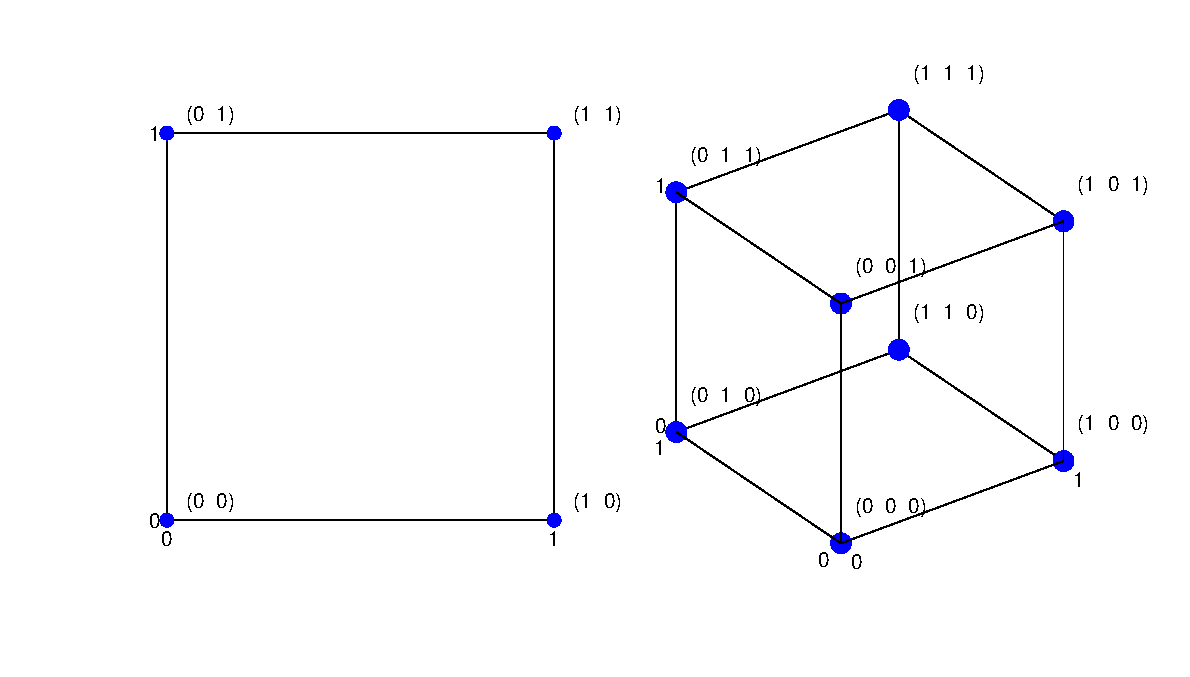
\includegraphics[width=4.5in]{figures/BernoulliDataSpace2and3}}
\end{figure}

\begin{definition}[Statistic]\label{D:Statistic}
A {\bf statistic} $T$ is any 
%(measurable) 
function of the data:
\[
T(x) : \Xz \to \Tz \ .
\]
Thus, a statistic $T$ is also an RV that takes values in the space $\Tz$.  When $x \in \Xz$ is the realisation of an experiment, we let $T(x)=t$ denote the corresponding realisation of the statistic $T$. Sometimes we use $T_n(X)$ and $\Tz_n$ to emphasise that $X$ is an $n$-dimensional random vector, i.e.~$\Xz \subset \Rz^n$ 
\end{definition}

\begin{classwork}[Is data a statistic?]
Is the RV $X$, for which the realisation is the observed data $X(\omega)=x$, a statistic?  In other words, is the data a statistic? [Hint: consider the identity map $T(x)=x: \Xz \to \Tz=\Xz$.]
\end{classwork}

Next, we define two important statistics called the {\bf sample mean} and {\bf sample variance}.  Since they are obtained from the sample data, they are called {\bf sample moments}, as opposed to the {\bf population moments}.  The corresponding population moments are $\e(X_1)$ and $\V(X_1)$, respectively.
\begin{definition}[Sample Mean]\label{D:SampleMean}
From a given a sequence of RVs $X_1,X_2,\ldots,X_n$, we may obtain another RV called the $n$-samples mean or simply the sample mean:
\begin{equation}\label{E:SampleMeanRV}
T_n( \ (X_1,X_2,\ldots,X_n) \ ) = \overline{X}_n( \ (X_1,X_2,\ldots,X_n) \ ) := \frac{1}{n} \sum_{i=1}^n X_i  \ .
\end{equation}
For brevity, we write $$\overline{X}_n( \ (X_1,X_2,\ldots,X_n) \ ) \quad \text{as} \quad \overline{X}_n \ ,$$ and its realisation $$\overline{X}_n( \ (x_1,x_2,\ldots,x_n) \ ) \quad \text{as} \quad \overline{x}_n \ .$$
\end{definition}
Note that the expectation and variance of $\overline{X}_n$ are:
\begin{eqnarray}
\e(\overline{X}_n) &=& \e \left(  \frac{1}{n} \sum_{i=1}^n X_i \right) \qquad \text{{\scriptsize[by \hyperref[E:SampleMeanRV]{definition \eqref{E:SampleMeanRV}}]}} \notag \\
&=&  \frac{1}{n} \sum_{i=1}^n \e \left( X_i \right) \qquad \text{{\scriptsize [by \hyperref[E:EofLinCombofRVs]{property \eqref{E:EofLinCombofRVs}}]}} \notag
\end{eqnarray}
Furthermore, if every $X_i$ in the original sequence of RVs $X_1,X_2,\ldots$ is {\bf identically} distributed with the same expectation, by convention $\e(X_1)$, then:
\begin{equation}\label{E:ExpOfSampleMeanOfIDSeq}
\e(\overline{X}_n) 
= \frac{1}{n} \sum_{i=1}^n \e \left( X_i \right)
=  \frac{1}{n} \sum_{i=1}^n \e \left( X_1 \right) 
=  \frac{1}{n} \ n \ \e \left( X_1 \right)  = \e \left( X_1 \right) \ .
\end{equation}
Similarly, we can show that:
\begin{eqnarray}
\V(\overline{X}_n) &=& \V \left(  \frac{1}{n} \sum_{i=1}^n X_i \right) \qquad \text{{\scriptsize[by \hyperref[E:SampleMeanRV]{definition \eqref{E:SampleMeanRV}}]}} \notag \\
&=& \left( \frac{1}{n} \right)^2  \V \left( \sum_{i=1}^n X_i \right) \qquad \text{{\scriptsize [by \hyperref[E:VofAffineofRVs]{property \eqref{E:VofAffineofRVs}}]}} \notag
\end{eqnarray}
Furthermore, if the original sequence of RVs $X_1,X_2,\ldots$ is {\bf independently} distributed then:
\begin{eqnarray}
\V(\overline{X}_n) 
= \left( \frac{1}{n} \right)^2 \V \left(  \sum_{i=1}^n X_i \right) 
=  \frac{1}{n^2} \ \sum_{i=1}^n \V \left( X_i \right) \qquad \text{{\scriptsize [by \hyperref[E:VofLinCombofRVs]{property \eqref{E:VofLinCombofRVs}}]}} \notag
\end{eqnarray}
Finally, if the original sequence of RVs $X_1,X_2,\ldots$ is {\bf independently and identically} distributed with the same variance ($\V(X_1)$ by convention) then:
\begin{equation}\label{E:VarOfSampleMeanOfIIDSeq}
\V(\overline{X}_n) 
=  \frac{1}{n^2} \ \sum_{i=1}^n \V \left( X_i \right)
= \frac{1}{n^2} \ \sum_{i=1}^n \V \left( X_1 \right)
=  \frac{1}{n^2} \ n \ \V \left( X_1 \right)
=  \frac{1}{n} \ \V \left( X_1 \right) \ .
\end{equation}

\begin{labwork}[Sample mean]\label{LW:XsFromUni01Twstr101mean}
After initializing the fundamental sampler, we draw five samples and then obtain the sample mean using the {\sc Matlab} function {\tt mean}.  In the following, we will reuse the samples stored in the array {\tt XsFromUni01Twstr101}.
\begin{VrbM}
>> rand('twister',101); % initialise the fundamental Uniform(0,1) sampler 
>> XsFromUni01Twstr101=rand(1,5); % simulate n=5 IID samples from Uniform(0,1) RV
>> SampleMean=mean(XsFromUni01Twstr101);% find sample mean
>> disp(XsFromUni01Twstr101); % The data-points x_1,x_2,x_3,x_4,x_5 are:
    0.5164    0.5707    0.0285    0.1715    0.6853
>> disp(SampleMean); % The Sample mean is :
    0.3945
\end{VrbM}
We can thus use {\tt mean} to obtain the sample mean $\overline{x}_n$ of $n$ sample points $x_1,x_2,\ldots,x_n$.

We may also obtain the sample mean using the {\tt sum} function and a division by sample size:
\begin{VrbM}
>> sum(XsFromUni01Twstr101) % take the sum of the elements of the XsFromUni01Twstr101 array
ans =    1.9723
>> sum(XsFromUni01Twstr101) / 5 % divide the sum by the sample size 5
ans =    0.3945
\end{VrbM}

We can also obtain the sample mean via matrix product or multiplication as follows:
\begin{VrbM}
>> size(XsFromUni01Twstr101) % size(SomeArray) gives the size or dimensions of the arrar SomeArray
ans =     1     5
>> ones(5,1) % here ones(5,1) is an array of 1's with size or dimension 5 X 1
ans =
     1
     1
     1
     1
     1
>> XsFromUni01Twstr101 * ones(5,1) % multiplying an 1 X 5 matrix with a 5 X 1 matrix of Ones
ans =    1.9723
>> XsFromUni01Twstr101 * ( ones(5,1) * 1/5) % multiplying an 1 X 5 matrix with a 5 X 1 matrix of 1/5 's
ans =    0.3945
\end{VrbM}
\end{labwork}

\begin{definition}[Sample Variance \& Standard Deviation]
From a given a sequence of random variables $X_1,X_2,\ldots,X_n$, we may obtain another statistic called the $n$-samples variance or simply the sample variance :
\begin{equation}\label{E:SampleVarianceRV}
T_n( \ (X_1,X_2,\ldots,X_n) \ ) = S^2_n( \ (X_1,X_2,\ldots,X_n) \ )  := \frac{1}{n-1} \sum_{i=1}^n {(X_i - \overline{X}_n)^2}  \ .
\end{equation}
For brevity, we write $S^2_n( \ (X_1,X_2,\ldots,X_n) \ )$ as $S^2_n$ and its  realisation $S^2_n( \ (x_1,x_2,\ldots,x_n) \ )$ as $s^2_n$.

Sample standard deviation is simply the square root of sample variance:
\begin{equation}\label{E:SampleStdDevRV}
S_n( \ (X_1,X_2,\ldots,X_n) \ ) = \sqrt{S^2_n( \ (X_1,X_2,\ldots,X_n) \ )}
\end{equation}
For brevity, we write $S_n( \ (X_1,X_2,\ldots,X_n) \ )$ as $S_n$ and its  realisation $S_n( \ (x_1,x_2,\ldots,x_n) \ )$ as $s_n$.
\end{definition}
Once again, if $X_1,X_2,\ldots,X_n \overset{\IID}{\sim} X_1$, the expectation of the sample variance is:
\[
\e(S^2_n) = \V(X_1) \ .
\]
\begin{labwork}[Sample variance and sample standard deviation]\label{LW:XsFromUni01Twstr101varstd}
We can compute the sample variance and sample standard deviation for the five samples stored in the array {\tt XsFromUni01Twstr101} from \hyperref[LW:XsFromUni01Twstr101mean]{Labwork \ref*{LW:XsFromUni01Twstr101mean}} using {\sc Matlab}'s functions {\tt var} and {\tt std}, respectively.
\begin{VrbM}
>> disp(XsFromUni01Twstr101); % The data-points x_1,x_2,x_3,x_4,x_5 are :
    0.5164    0.5707    0.0285    0.1715    0.6853
>> SampleVar=var(XsFromUni01Twstr101);% find sample variance
>> SampleStd=std(XsFromUni01Twstr101);% find sample standard deviation
>> disp(SampleVar) % The sample variance is:
    0.0785
>> disp(SampleStd) % The sample standard deviation is:
    0.2802
\end{VrbM}
\end{labwork}
It is important to bear in mind that the statistics such as sample mean and sample variance are random variables and have an underlying distribution.

\begin{definition}[Order Statistics]
Suppose $X_1,X_2,\ldots,X_n \overset{\IID}{\sim} F$, where $F$ is the DF from the set of all DFs over the real line.  Then, the $n$-sample {\bf order statistics} $X_{([n])}$ is:
\begin{equation}\label{E:OrderStatistics}
X_{([n])}( \ (X_1,X_2,\ldots,X_n) \ ) := \left(  X_{(1)},X_{(2)}, \ldots X_{(n)} \right), \text{ such that, }
 X_{(1)} \leq X_{(2)} \leq \ldots \leq X_{(n)}  \ .
\end{equation}
For brevity, we write $X_{([n])}( \ (X_1,X_2,\ldots,X_n) \ )$ as $X_{([n])}$ and its realisation $X_{([n])}( \ (x_1,x_2,\ldots,x_n) \ )$ as $x_{([n])} = (  x_{(1)},x_{(2)}, \ldots x_{(n)} )$.
\end{definition}
Without going into the details of how to sort the data in ascending order to obtain the order statistics (an elementary topic of an Introductory Computer Science course), we simply use {\sc Matlab}'s function {\tt sort} to obtain the order statistics, as illustrated in the following example.
\begin{labwork}[Order statistics and sorting]\label{LW:SortedXsFromUni01Twstr101}
The order statistics for the five samples stored in {\tt XsFromUni01Twstr101} from \hyperref[LW:XsFromUni01Twstr101mean]{Labwork \ref*{LW:XsFromUni01Twstr101mean}} can be computed using {\tt sort} as follows:
\begin{VrbM}
>> disp(XsFromUni01Twstr101); % display the sample points
    0.5164    0.5707    0.0285    0.1715    0.6853
>> SortedXsFromUni01Twstr101=sort(XsFromUni01Twstr101); % sort data
>> disp(SortedXsFromUni01Twstr101); % display the order statistics
    0.0285    0.1715    0.5164    0.5707    0.6853
\end{VrbM}
Therefore, we can use {\tt sort} to obtain our order statistics $x_{(1)},x_{(2)},\ldots,x_{(n)}$ from $n$ sample points $x_1,x_2,\ldots,x_n$.
\end{labwork}

Next, we will introduce a family of common statistics, called the $q^{\text{th}}$ quantile, by first defining the function:
\begin{definition}[Inverse DF or Inverse CDF or Quantile Function]
Let $X$ be an RV with DF $F$.  The {\bf inverse DF} or {\bf inverse CDF} or {\bf quantile function} is:
\begin{equation}\label{E:InverseCDF}
F^{[-1]}(q) := \inf { \{ x: F(x) > q \}}, \quad \text{ for some $q \in [0,1]$} \ .
\end{equation} 
If $F$ is strictly increasing and continuous then $F^{[-1]}(q)$ is the unique $x \in \Rz$ such that $F(x)=q$.
\end{definition}
A {\bf functional} is merely a function of another function.  Thus, $T(F): \{ \text{All DFs }\} \to \Tz$, being a map or function from the space of DFs to its range $\Tz$, is a functional.  Some specific examples of functionals we have already seen include:
\begin{enumerate}
\item The {\bf mean} of RV $X \sim F$ is a function of the DF $F$:  
\[
T(F) = \e(X) = \int x\,dF(x) \ .
\]
\item The {\bf variance} of RV $X \sim F$ is a function of the DF $F$:  
\[
T(F) = \e(X-\e(X))^2 = \int (x-\e(X))^2\,dF(x) \ .
\]
\item The {\bf value of DF at a given $x \in \Rz$} of RV $X \sim F$ is also a function of DF $F$:
\[
T(F) = F(x) \  .
\]
\end{enumerate}
Other functionals of $F$ that depend on the quantile function $F^{[-1]}$ are:
\begin{enumerate}
\item The {\bf $q^{\text{th}}$ quantile} of RV $X \sim F$: 
\[
T(F) = F^{[-1]}(q) \ \text{ where } q \in [0,1] \ .
\]
\item The {\bf first quartile} or the {\bf $0.25^{\text{th}}$ quantile} of the RV $X \sim F$: 
\[
T(F) = F^{[-1]}(0.25) \ .
\]
\item The {\bf median} or the {\bf second quartile} or the {\bf $0.50^{\text{th}}$ quantile} of the RV $X \sim F$: 
\[
T(F) = F^{[-1]}(0.50) \  .
\]
\item The {\bf third quartile} or the {\bf $0.75^{\text{th}}$ quantile} of the RV $X \sim F$: 
\[
T(F) = F^{[-1]}(0.75) \ .
\]
\end{enumerate}

\begin{definition}[Empirical Distribution Function (EDF or ECDF)]\label{D:ECDF}
Suppose we have $n$ IID RVs, $X_1,X_2,\ldots,X_n \overset{\IID}{\sim} F$, where $F$ is a DF from the set of all DFs over the real line.  Then, the $n$-sample empirical distribution function (EDF or ECDF) is the discrete  distribution function $\widehat{F}_n$ that puts a probability mass of $1/n$ at each sample or data point $x_i$:
\begin{eqnarray} \label{E:ECDF}
\widehat{F}_n(x) = \frac{ \sum_{i=1}^n \BB{1}(X_i \leq x) }{n} \ ,  & \quad where \qquad
\BB{1}(X_i \leq x) :=
\begin{cases}
& 1  \quad \text{if $x_i \leq x$} \\
& 0  \quad \text{if $x_i > x$} 
\end{cases}
\end{eqnarray}
\end{definition}

\begin{labwork}[Plot of empirical CDF]\label{LW:ECDF}
Let us plot the ECDF for the five samples drawn from the $Uniform(0,1)$ RV in \hyperref[LW:XsFromUni01Twstr101mean]{Labwork \ref*{LW:XsFromUni01Twstr101mean}} using the {\sc Matlab} function {\tt ECDF}. %(given in \hyperref[Mf:ECDF]{Labwork \ref*{Mf:ECDF}}).  
Let us super-impose the samples and the true DF as depicted in \hyperref[F:plotUniform01ECDF5]{Figure \ref*{F:plotUniform01ECDF5}} with the following script:
{\VrbMf[label=plotunifecdf.m]{scripts/plotunifecdf.m}}

\begin{figure}[htpb]
\caption{Plot of the DF of $\uniform(0,1)$, five IID samples from it, and the ECDF $\widehat{F}_5$ for these five data points $x=(x_1,x_2,x_3,x_4,x_5)=(0.5164,    0.5707,    0.0285,    0.1715,    0.6853)$ that jumps by $1/5=0.20$ at each of the five samples.\label{F:plotUniform01ECDF5}}
\centering   \makebox{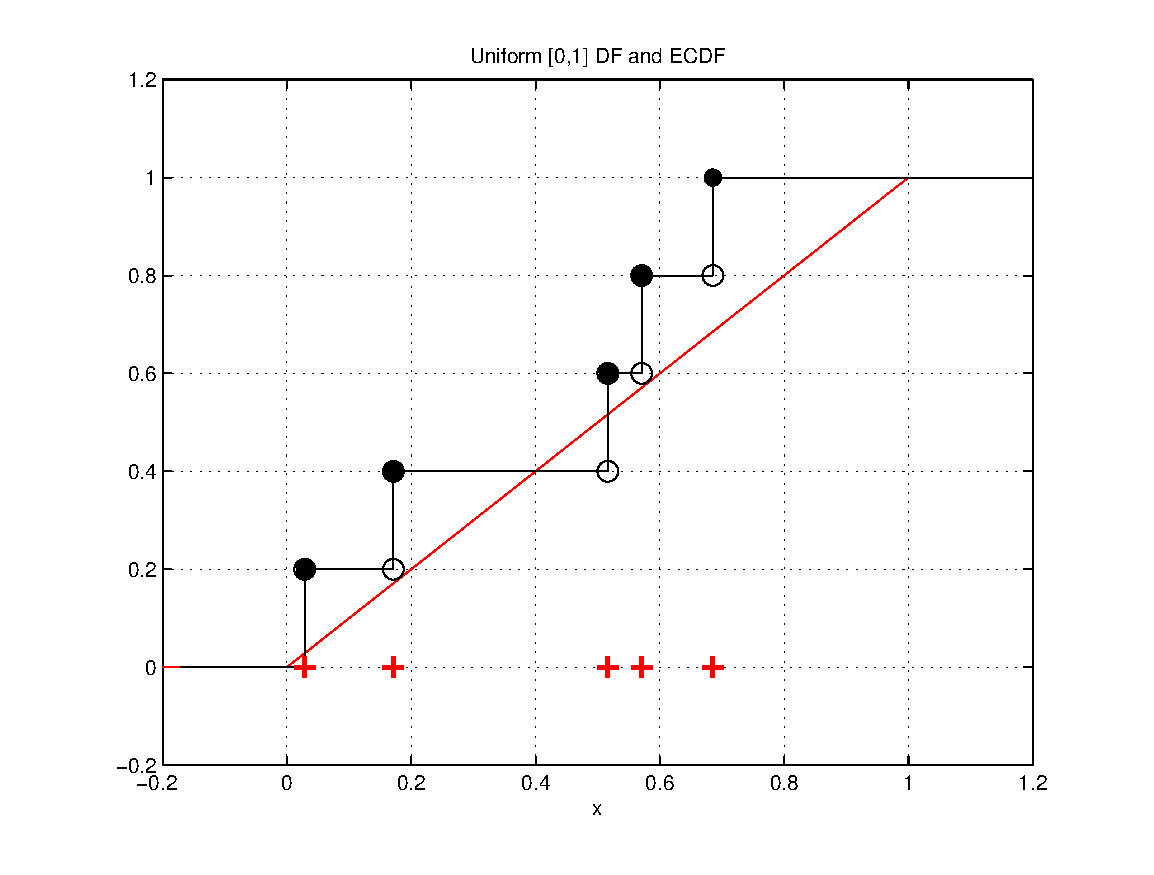
\includegraphics[width=4.5in]{figures/plotUniform01ECDF5}}
\end{figure}
\end{labwork}

\begin{definition}[$q^{\text{th}}$ Sample Quantile]
For some $q \in [0,1]$ and $n$ IID RVs $X_1,X_2,\ldots,X_n \overset{\IID}{\sim} F$, we can obtain the ECDF $\widehat{F}_n$ using \eqref{E:ECDF}.  The {\bf $q^{\text{th}}$ sample quantile} is defined as the statistic (statistical functional):
\begin{equation}\label{E:qthSampleQuantile}
T(\widehat{F}_n) = \widehat{F}_n^{[-1]}(q) := \inf{ \{ x:  \widehat{F}_n^{[-1]}(x) \geq q \} } \ .
\end{equation}
By replacing $q$ in this definition of the $q^{\text{th}}$ sample quantile by $0.25$, $0.5$ or $0.75$, we obtain the first, second ({\bf sample median}) or third {\bf sample quartile}, respectively.
\end{definition}

The following algorithm can be used to obtain the $q^{\text{th}}$ sample quantile of $n$ IID samples $(x_1,x_2,\ldots,x_n)$ on the basis of their order statistics $(x_{(1)},x_{(2)},\ldots,x_{(n)})$.
\begin{algorithm}
\caption{$q^{\text{th}}$ Sample Quantile of Order Statistics}
\label{A:qthSampleQuantile}
\begin{algorithmic}[1]
\STATE {
{\it input:} 
\begin{enumerate}
\item $q$ in the $q^{\text{th}}$ sample quantile, i.e.~the argument $q$ of $ \widehat{F}_n^{[-1]}(q)$,
\item order statistic $(x_{(1)},x_{(2)},\ldots,x_{(n)})$, i.e.~the sorted $(x_1,x_2,\ldots,x_n)$, where $n>0$.
\end{enumerate}
}
\STATE {\it output:} $ \widehat{F}_n^{[-1]}(q)$, the $q^{\text{th}}$ sample quantile
\STATE $i \gets \lfloor (n-1) q \rfloor$
\STATE $\delta \gets (n-1) q - i$
\IF {$i = n-1$}
\STATE {$ \widehat{F}_n^{[-1]}(q) \gets x_{(i+1)}$}
\ELSE
\STATE $ \widehat{F}_n^{[-1]}(q) \gets (1 - \delta) x_{(i+1)} + \delta x_{(i+2)}$
\ENDIF
\STATE {{\it return:} $ \widehat{F}_n^{[-1]}(q)$}
\end{algorithmic}
\end{algorithm}

The $q^{\text{th}}$ sample quantile, $ \widehat{F}_n^{[-1]}(q)$, is found by interpolation from the order statistics $(x_{(1)},x_{(2)},\ldots,x_{(n)})$ of the $n$ data points $(x_1,x_2,\ldots,x_n)$, using the formula:
\[
 \widehat{F}_n^{[-1]}(q) = (1 - \delta) x_{(i+1)} + \delta x_{(i+2)}, \quad \text{where, }
\quad i = \lfloor (n-1) q \rfloor  \quad \text{ and }
\quad \delta = (n-1) q -  \lfloor (n-1) q \rfloor \ .
\]
Thus, the {\bf sample minimum} of the data points $(x_1,x_2,\ldots,x_n)$ is given by $ \widehat{F}_n^{[-1]}(0)$, the {\bf sample maximum} is given by $ \widehat{F}_n^{[-1]}(1)$ and the {\bf sample median} is given by $ \widehat{F}_n^{[-1]}(0.5)$, etc.
\begin{labwork}[The $q^{\text{th}}$ sample quantile]\label{LW:qthSampleQuantile}
Use the implementation of \hyperref[A:qthSampleQuantile]{Algorithm \ref*{A:qthSampleQuantile}} %in \hyperref[Mf:qthSampleQuantile]{Labwork \ref*{Mf:qthSampleQuantile}} 
as the {\sc Matlab} function {\tt qthSampleQuantile} to find the $q^{\text{th}}$ sample quantile of two simulated data arrays:
\begin{enumerate}
\item {\tt SortedXsFromUni01Twstr101}, the order statistics that was constructed in \hyperref[LW:SortedXsFromUni01Twstr101]{Labwork \ref*{LW:SortedXsFromUni01Twstr101}} and
\item Another sorted array of $7$ samples called {\tt SortedXs}
\end{enumerate}
\begin{VrbM}
>> disp(SortedXsFromUni01Twstr101)
    0.0285    0.1715    0.5164    0.5707    0.6853
>> rand('twister',420);
>> SortedXs=sort(rand(1,7));
>> disp(SortedXs)
    0.1089    0.2670    0.3156    0.3525    0.4530    0.6297    0.8682
>> for q=[0, 0.25, 0.5, 0.75, 1.0]
       disp([q, qthSampleQuantile(q,SortedXsFromUni01Twstr101) ...
                qthSampleQuantile(q,SortedXs)])
   end
         0    0.0285    0.1089
    0.2500    0.1715    0.2913
    0.5000    0.5164    0.3525
    0.7500    0.5707    0.5414
    1.0000    0.6853    0.8682
\end{VrbM}
\end{labwork}

%\subsection{Exploring Data and Statistics}\label{S:ExploringData}

\subsection{Univariate Data}
A {\bf histogram} is a graphical representation of the frequency with which elements of a data array:
$$x = (x_1,x_2,\ldots,x_n) \ ,$$ 
of real numbers fall within each of the $m$ intervals or {\bf bins} of some {\bf interval partition}:
$$b := ( b_1, b_2, \ldots, b_m ) := ( [\underline{b}_1,\overline{b}_1], [\underline{b}_2,\overline{b}_2], \ldots, [\underline{b}_m,\overline{b}_m] )$$
of the {\bf data range} of $x$ given by the closed interval: 
$$\C{R}(x) := [\min \{x_1,x_2,\ldots,x_n \}, \max \{x_1,x_2,\ldots,x_n \}] \ .$$  
Elements of this partition $b$ are called bins, their mid-points are called {\bf bin centres}:
$$c := ( c_1, c_2, \ldots, c_m ) := ( (\underline{b}_1+\overline{b}_1)/2, (\underline{b}_2 + \overline{b}_2)/2, \ldots, (\underline{b}_m + \overline{b}_m)/2 )$$
and their overlapping boundaries, i.e.~$\overline{b}_i=\underline{b}_{i+1}$ for $1 \leq i < m$, are called {\bf bin edges}:
$$d := (d_1,d_2,\ldots,d_{m+1}) := (\underline{b}_1, \underline{b}_2, \ldots, \underline{b}_{m-1}, \underline{b}_m, \overline{b}_m) \ .$$ 
For a given partition of the data range $\C{R}(x)$ or some superset of $\C{R}(x)$, three types of histograms are possible: frequency histogram, relative frequency histogram and density histogram.  Typically, the partition $b$ is assumed to be composed of $m$ overlapping intervals of the same width $w=\overline{b}_i - \underline{b}_i$ for all $i=1,2,\ldots,m$.  Thus, a histogram can be obtained by a set of bins along with their corresponding {\bf heights}:
$$h = (h_1,h_2,\ldots,h_m) \ , \text{ where } h_k := g(\# \{x_i : x_i \in b_k\} )$$
Thus, $h_k$, the height of the $k$-th bin, is some function $g$ of the number of data points that fall in the bin $b_k$ Formally, a histogram is a sequence of ordered pairs:
$$\left(  (b_1,h_1), (b_2,h_2), \ldots, (b_m,h_m) \right) \ .$$

Given a partition $b$, a {\bf frequency histogram} is the histogram:
$$\left(  (b_1,h_1), (b_2,h_2), \ldots, (b_m,h_m) \right) \ , \text{ where } h_k := \# \{x_i : x_i \in b_k\} \ ,$$
a {\bf relative frequency histogram} is the histogram:
$$\left(  (b_1,h_1), (b_2,h_2), \ldots, (b_m,h_m) \right) \ , \text{ where } h_k := n^{-1} \# \{x_i : x_i \in b_k\} \ ,$$
and a {\bf density histogram} is the histogram:
$$\left(  (b_1,h_1), (b_2,h_2), \ldots, (b_m,h_m) \right) \ , \text{ where } h_k := (w_k n)^{-1} \# \{x_i : x_i \in b_k\} \ , w_k := \overline{b}_k - \underline{b}_k \ .$$
  
\begin{figure}[htpb]
\caption{Frequency, Relative Frequency and Density Histograms\label{F:FreqRelFreqDensityHistograms100Unif01MT5489}}
\centering   \makebox{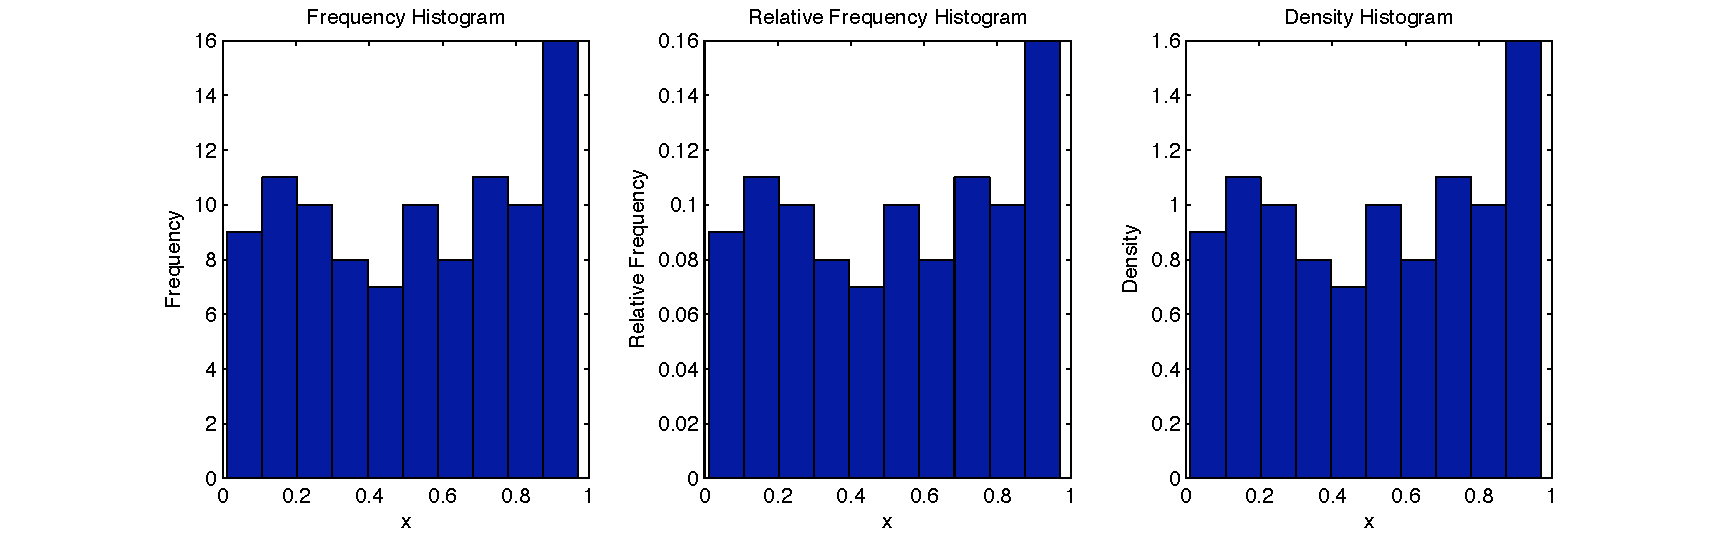
\includegraphics[width=6.5in]{figures/FreqRelFreqDensityHistograms100Unif01MT5489}}
\end{figure}

\begin{labwork}[Histograms with specified number of bins for univariate data]\label{LW:hist}
Let us use samples from the {\tt rand('twister',5489)} as our data set $x$ and plot various histograms.  Let us use {\tt hist} function (read {\tt help hist}) to make a default histogram with ten bins.  Then we can make three types of histogarms as shown in \hyperref[F:FreqRelFreqDensityHistograms100Unif01MT5489]{Figure~\ref*{F:FreqRelFreqDensityHistograms100Unif01MT5489}}  as follows:
\begin{VrbM}
>> rand('twister',5489);
>> x=rand(1,100); % generate 100 PRNs
>> hist(x) % see what default hist does in Figure Window
>> % Now let us look deeper into the last hist call
>> [Fs, Cs] = hist(x) % Cs is the bin centers and Fs is the frequencies of data set x
Fs =
     9    11    10     8     7    10     8    11    10    16
Cs =
    0.0598    0.1557    0.2516    0.3474    0.4433    0.5392    0.6351    0.7309    0.8268    0.9227
>> % produce a histogram plot the last argument 1 is the width value for immediately adjacent bars -- help bar
>> bar(Cs,Fs,1) % create a frequency histogram
>> bar(Cs,Fs/100,1) % create a relative frequency histogram
>> bar(Cs,Fs/(0.1*100),1) % create a density histogram (area of bars sum to 1)
>> sum(Fs/(0.1*100) .* ones(1,10)*0.1) % checking if area does sum to 1
>> ans = 1
\end{VrbM}
Try making a density histogram with 1000 samples from {\tt rand} with 15 bins.  You can specify the number of bins by adding an extra argument to {\tt hist}, for e.g. {\tt [Fs, Cs] = hist(x,15)} will produce 15 bins of equal width over the data range $\C{R}(x)$.
\end{labwork}

\begin{labwork}[Stem plots and ECDF plots for univariate data]\label{LW:StemEcdf}
We can also visualise the 100 data points in the array {\tt x} using stem plot and ECDF plot as shown in \hyperref[F:StemECDF100Unif01MT5489]{Figure~\ref*{F:StemECDF100Unif01MT5489}} as follows:
\begin{VrbM}
>> rand('twister',5489);
>> x=rand(1,100); % produce 100 samples with rand
>> stem(x,'.') % make a stem plot of the 100 data points in x (the option '.' gives solid circles for x)
>>% ECDF (type help ECDF) plot is extended to left and right by .2 and .6, respectively
>>% (second parameter 6 makes the dots in the plot smaller).
>> ECDF(x,6,.2,.6);
\end{VrbM}
\end{labwork}

\begin{figure}[htpb]
\caption{Frequency, Relative Frequency and Density Histograms\label{F:StemECDF100Unif01MT5489}}
\centering   \makebox{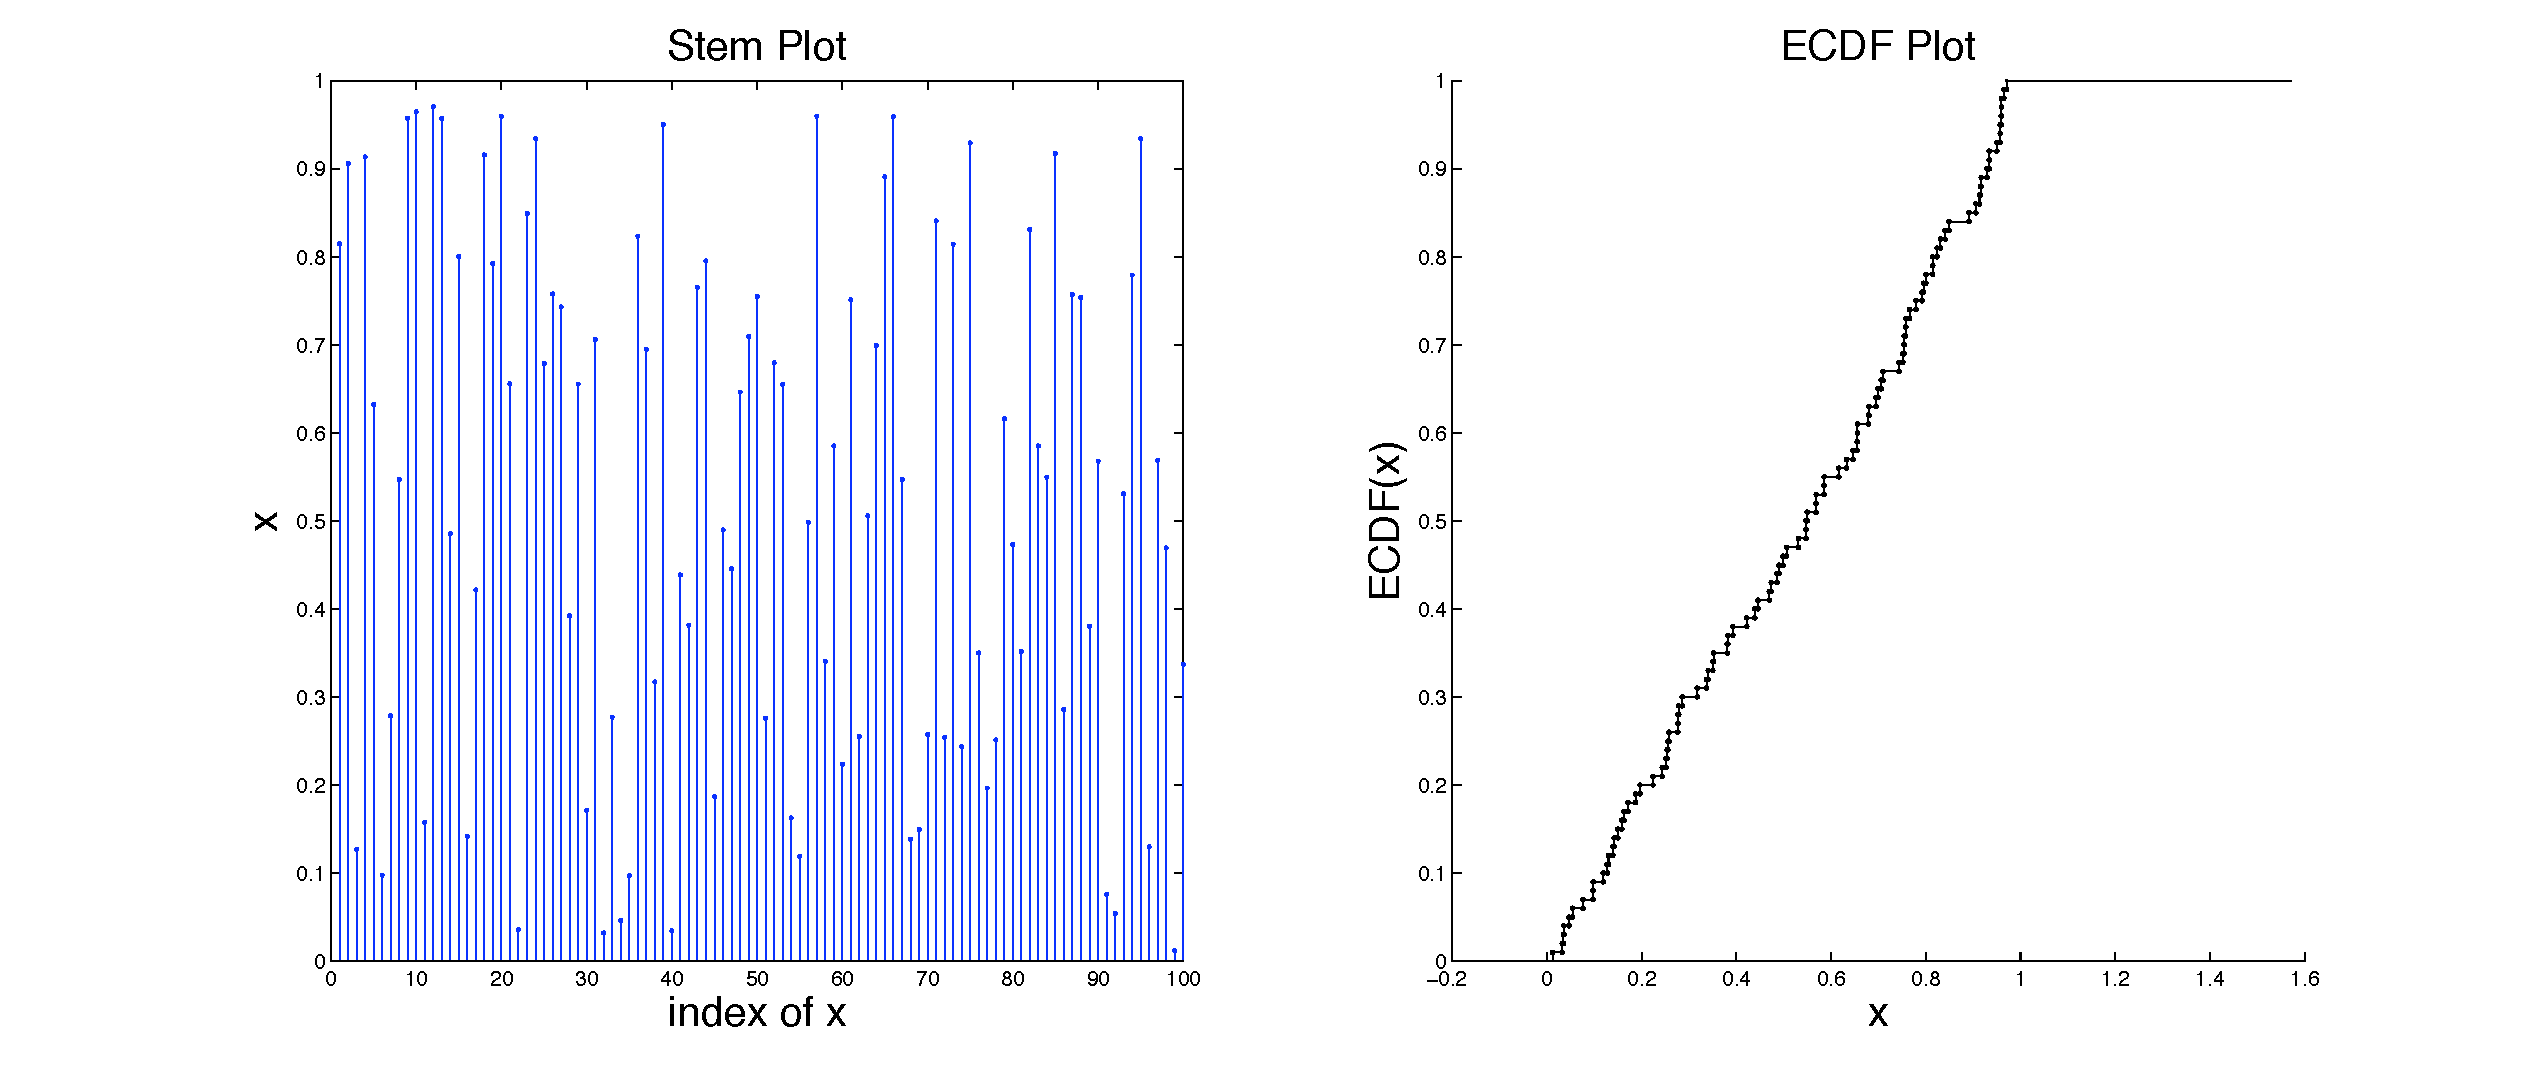
\includegraphics[width=6.5in]{figures/StemECDF100Unif01MT5489}}
\end{figure}

We can also visually summarise univariate data using the {\bf box plot} or {\bf box-whisker plot} available in the Stats Toolbox of {\sc Matlab}.  These family of plots display a set of sample quantiles, typically they are include, the median, the first and third quartiles and the minimum and maximum values of our data array $x$.

\subsection{Bivariate Data}
By bivariate data array $x$ we mean a $2 \times n$ matrix of real numbers or equivalently $n$ ordered pairs of points $(x_{1,i},x_{2,i})$ as $i=1,2,\ldots,n$.  The most elementary visualisation of these $n$ ordered pairs is in orthogonal Cartesian co-ordinates.  Such plots are termed 2D {\bf scatter plots} in statistics.
\begin{labwork}[Visualising bivariate data]\label{LW:2DScatter}
Let us generate a $2 \times 5$ array representing samples of $5$ ordered pairs sampled uniformly at random over the unit square $[0,1] \times [0,1]$.  We can make 2D scatter plot as shown in \hyperref[F:Twister5489X2x5Scatter2D]{Figure~\ref*{F:Twister5489X2x5Scatter2D}}  as follows:
\begin{VrbM}
>> rand('twister',5489);
>> x=rand(2,5)% create a sequence of 5 ordered pairs uniformly from unit square [0,1]X[0,1]
x =
    0.8147    0.1270    0.6324    0.2785    0.9575
    0.9058    0.9134    0.0975    0.5469    0.9649
>> plot(x(1,:),x(2,:),'x') % a 2D scatter plot with marker cross or 'x'
>> plot(x(1,:),x(2,:),'x', 'MarkerSize',15) % a 2D scatter plot with marker cross or 'x' and larger Marker size
>> xlabel('x_1'); ylabel('x_2'); % label the axes
\end{VrbM}
\end{labwork}

\begin{figure}[htpb]
\caption{2D Scatter Plot\label{F:Twister5489X2x5Scatter2D}}
\centering   \makebox{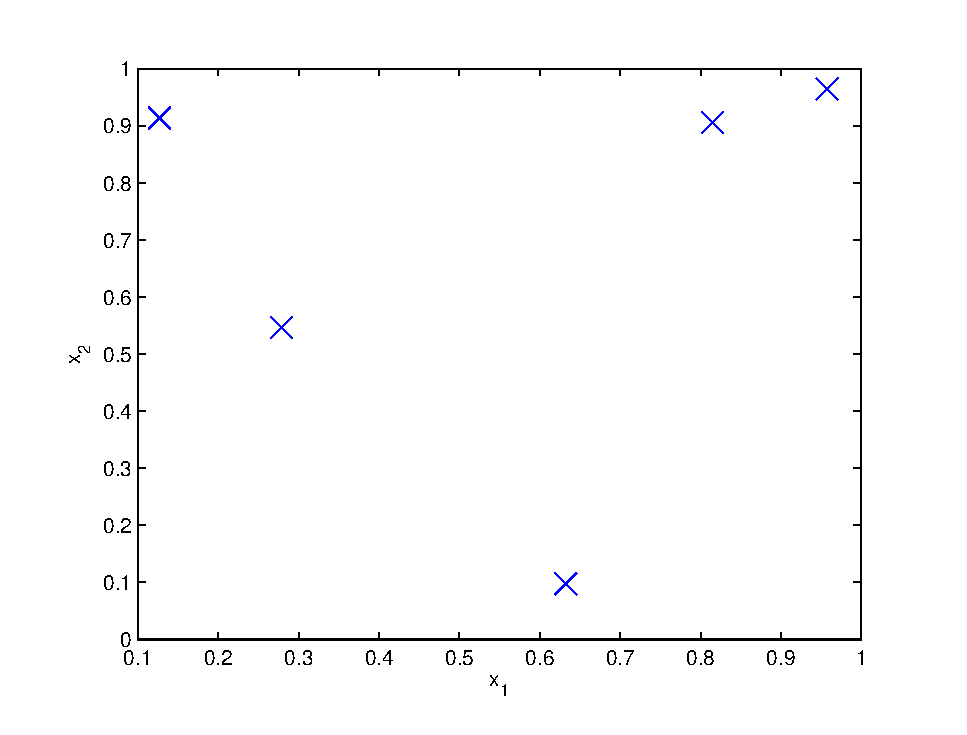
\includegraphics[width=4.5in]{figures/Twister5489X2x5Scatter2D}}
\end{figure}

There are several other techniques for visualising bivariate data, including,
2D histograms, surface plots, heat plots, and we will encounter some of them in the sequel.

\subsection{Trivariate Data}
Trivariate data is more difficult to visualise on paper but playing around with the rotate 3D feature in \Matlab's Figure window can help bring a lot more perspective.

\begin{labwork}[Visualising trivariate data]\label{LW:3DScatter}
We can make {\bf 3D scatter plots} as shown in \hyperref[F:Twister5489X3x5Scatter3D]{Figure~\ref*{F:Twister5489X3x5Scatter3D}}  as follows:
\begin{VrbM}
>> rand('twister',5489);
>> x=rand(3,5)% create a sequence of 5 ordered triples uniformly from unit cube [0,1]X[0,1]X[0,1]
x =
    0.8147    0.9134    0.2785    0.9649    0.9572
    0.9058    0.6324    0.5469    0.1576    0.4854
    0.1270    0.0975    0.9575    0.9706    0.8003
>> plot3(x(1,:),x(2,:),x(3,:),'x') % a simple 3D scatter plot with marker 'x'
>>% a more interesting one with options that control marker type, line-style, 
>>% colour in [Red Green Blue] values and marker size - read help plot3 for more options
>> plot3(x(1,:),x(2,:),x(3,:),'Marker','*','LineStyle','none','Color',[1 0 1],'MarkerSize',15) 
>> plot3(x(1,:),x(2,:),x(3,:),'m*','MarkerSize',15) % makes same  figure as before but shorter to write
>> box on % turn on the box and see the effect on the Figure
>> grid on % turn on the grid and see the effect on the Figure
>> xlabel('x_1'); ylabel('x_2'); zlabel('x_3'); % assign labels to x,y and z axes
\end{VrbM}
Repeat the visualisation below with a larger array, say {\tt x=rand(3,1000)}, and use the rotate 3D feature in the Figure window to visually explore the samples in the unit cube.  Do they seem to be uniformly distributed inside the unit cube?
\end{labwork}

\begin{figure}[htpb]
\caption{3D Scatter Plot\label{F:Twister5489X3x5Scatter3D}}
\centering   \makebox{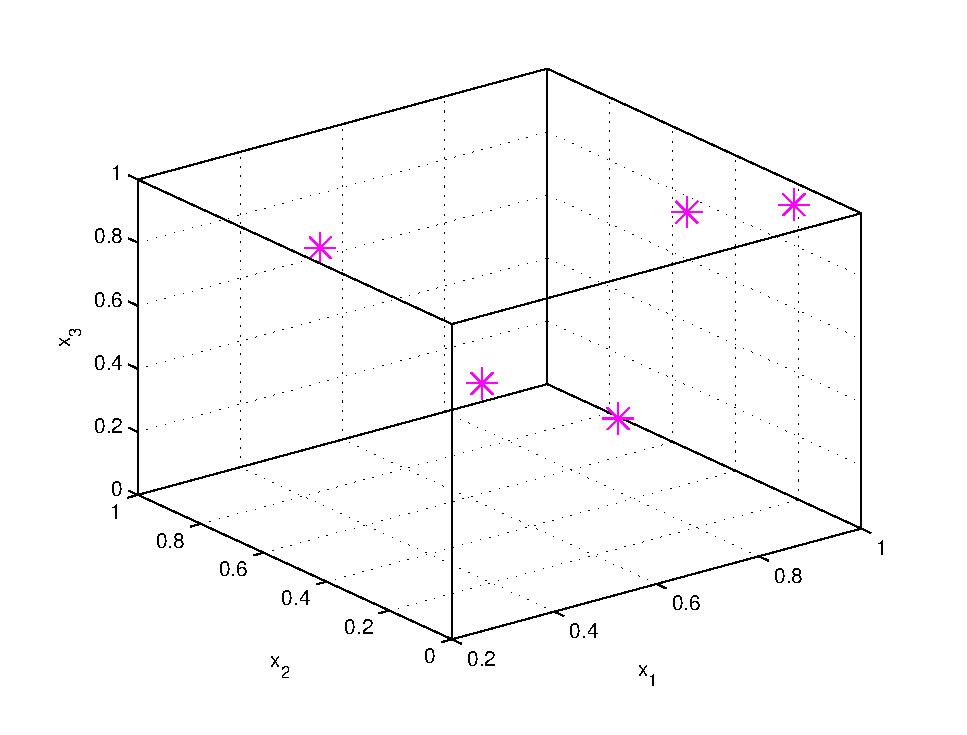
\includegraphics[width=4.5in]{figures/Twister5489X3x5Scatter3D}}
\end{figure}


There are several other techniques for visualising trivariate data, including,
iso-surface plots, moving surface or heat plots, and you will encounter some of them in the future.

\subsection{Multivariate Data}
For high-dimensional data in $d$-dimensional space $\Rz^d$ with $d \geq 3$ you have to look at several lower dimensional projections of the data.  We can simultaneously look at 2D scatter plots for every pair of co-ordinates $\{(i,j) \in \{1,2,\ldots,d\}^2 : i \neq j \}$ and at histograms for every co-ordinate $i \in \{1,2,\ldots,d\}$ of the $n$ data points in $\Rz^d$.  Such a set of low-dimensional projections can be conveniently represented in a $d \times d$ matrix of plots called a {\bf matrix plot}. 

\begin{figure}[htpb]
\caption{Plot Matrix of uniformly generated data in $[0,1]^5$\label{F:Twister5489X100x5PlotMatrixFirst6andAll100}}
\centering
\mbox{\subfigure[First six samples]{\hspace{-1.cm} 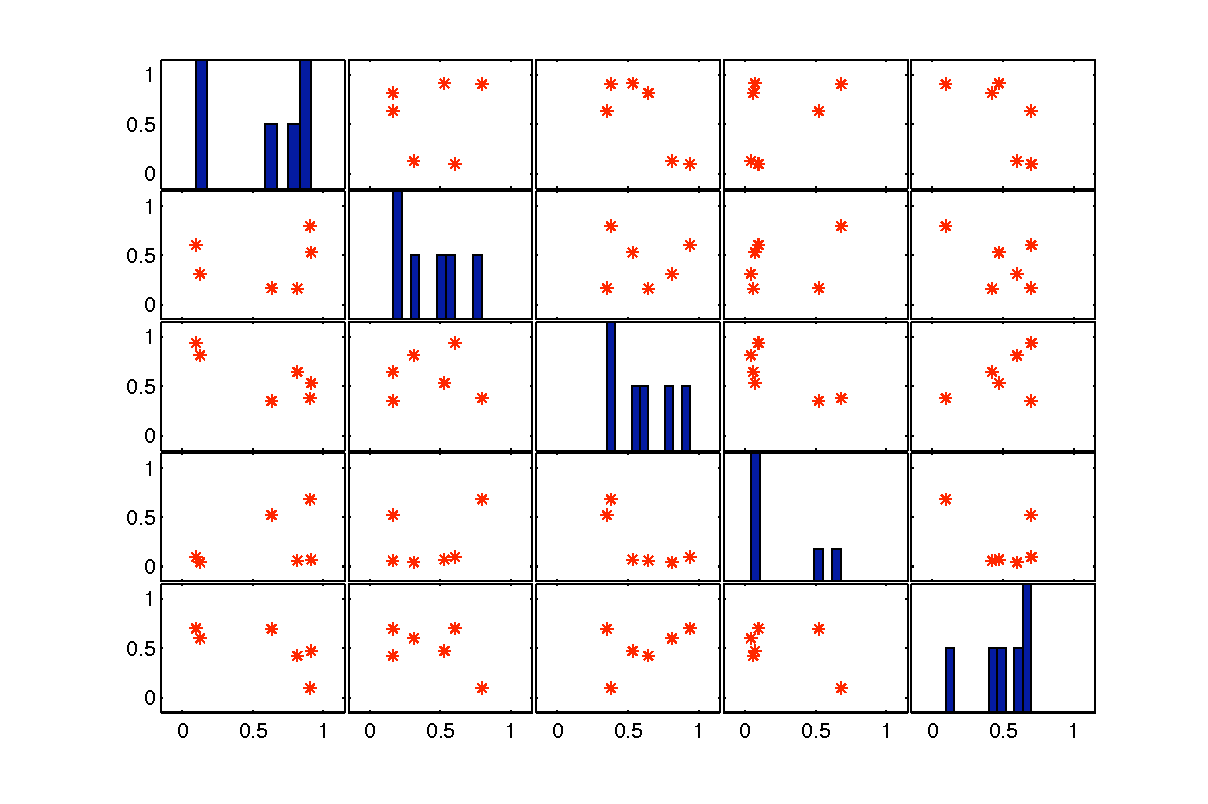
\includegraphics[width=3.750in]{figures/Twister5489X100x5PlotMatrixFirst6}} \hspace{-1.cm}
	   \subfigure[All thousand samples]{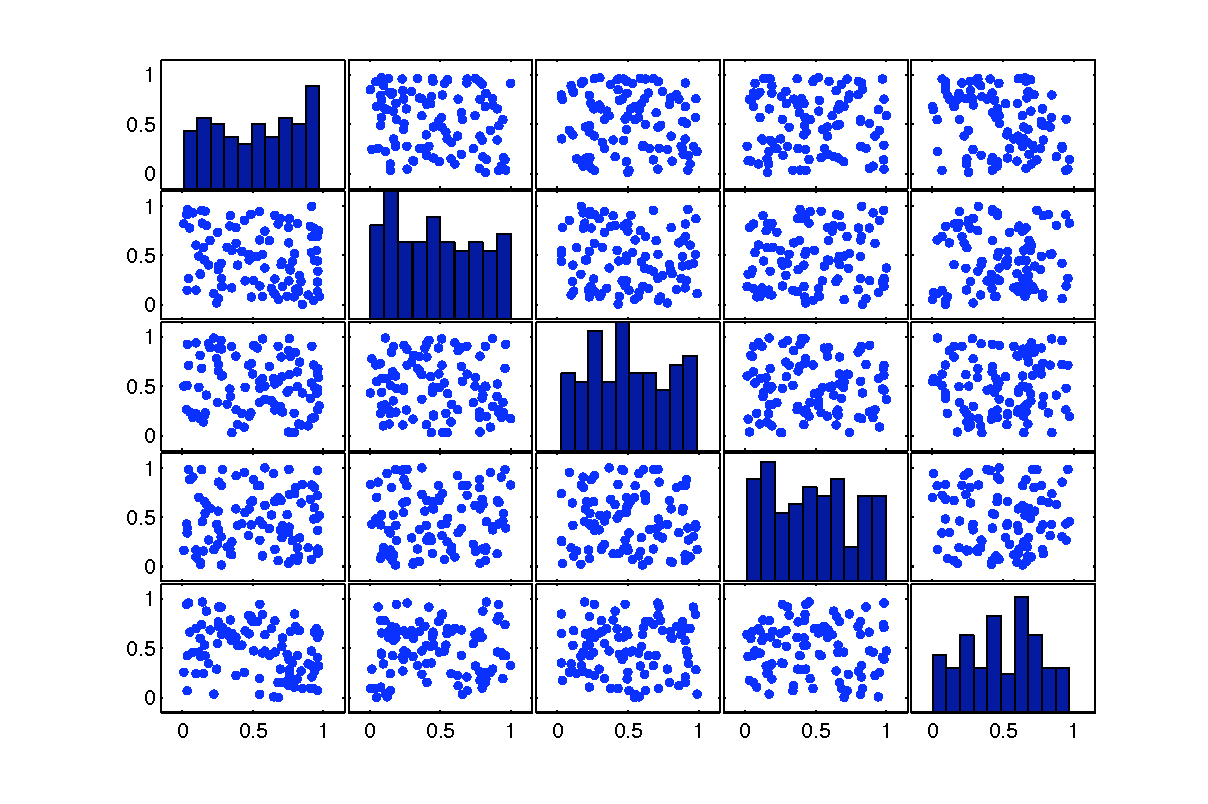
\includegraphics[width=3.750in]{figures/Twister5489X100x5PlotMatrixAll100}} }
\end{figure}

\begin{labwork}\label{LW:matrixplot5DUniform}
Let us make matrix plots from a uniformly generated  sequence of $100$ points in 5D unit cube $[0,1]^5$ as shown in \hyperref[F:Twister5489X100x5PlotMatrixFirst6andAll100]{Figure~\ref*{F:Twister5489X100x5PlotMatrixFirst6andAll100}}.
\begin{VrbM}
>> rand('twister',5489);
>> % generate a sequence of 1000 points uniformly distributed in 5D unit cube [0,1]X[0,1]X[0,1]X[0,1]X[0,1]
>> x=rand(1000,5);
>> x(1:6,:) % first six points in our 5D unit cube, i.e., the first six rows of x
ans =
    0.8147    0.6312    0.7449    0.3796    0.4271
    0.9058    0.3551    0.8923    0.3191    0.9554
    0.1270    0.9970    0.2426    0.9861    0.7242
    0.9134    0.2242    0.1296    0.7182    0.5809
    0.6324    0.6525    0.2251    0.4132    0.5403
    0.0975    0.6050    0.3500    0.0986    0.7054
>> plotmatrix(x(1:5,:),'r*') % make a plot matrix
>> plotmatrix(x) % make a plot matrix of all 1000 points
\end{VrbM}
\end{labwork}


\subsection{Loading and Exploring Real-world Data}\label{S:EDA}

All of the data we have played with so far were computer-generated.  It is time to get our hands dirty with real-world data.  The first step is to obtain the data.  
Often, publicly-funded institutions allow the public to access their databases.  Such data can be fetched from appropriate URLs in one of the two following ways: 
\begin{itemize}
\item[{\sf Method~A}:] Manually download by filling the appropriate fields in an online request form.
\item[{\sf Method~B}:] Automagically download directly from your \Matlab session.
\end{itemize}
Then we want to inspect it for inconsistencies, missing values and replace them with {\tt NaN} values in \Matlab that stand for not-any-number.  Finally, we can visually explore, transform and interact with the data to discover interesting patterns that are hidden in the data.  This process is called {\em exploratory data analysis} and is the foundational first step towards subsequent computational statistical experiments [{\em John W.~Tukey, Exploratory Data Analysis, Addison-Wesely, New York, 1977}].

\subsection{Geological Data}
 Let us focus on the data of earth quakes that heavily damaged Christchurch on February 22 2011.  This data can be fetched from the URL \href{http://magma.geonet.org.nz/resources/quakesearch/}{\url{http://magma.geonet.org.nz/resources/quakesearch/}} by {\sf Method A} and loaded into \Matlab for exploratory data analysis as done in \hyperref[LW:NZEQChCch20110222]{Labwork~\ref*{LW:NZEQChCch20110222}}.
 
 \begin{labwork}\label{LW:NZEQChCch20110222}
Let us go through the process one step at a time using {\sf Method~A}.  
\begin{enumerate}
\item Download the data as a CSV or {\em comma separated variable} file in plain ASCII text (this has been done for this data already for you and saved as {\tt NZ20110222earthquakes.csv} in the {\tt CSEMatlabScripts} directory).
\item Open the file in a simple text editor such as {\tt Note Pad} in Windows or one of the following editors in OS X, Unix, Solaris, Linux/GNU variants such as Ubuntu, SUSE, etc: {\tt vi}, {\tt vim}, {\tt emacs}, {\tt geany}, etc.  The first three and last two lines of this file look as follows:
\begin{VrbM} 
CUSP_ID,LAT,LONG,NZMGE,NZMGN,ORI_YEAR,ORI_MONTH,ORI_DAY,ORI_HOUR,ORI_MINUTE,ORI_SECOND,MAG,DEPTH
3481751,-43.55432,172.68898,2484890,5739375,2011,2,22,0,0,31.27814,3.79,5.8559,
3481760,-43.56579,172.70621,2486287,5738106,2011,2,22,0,0,43.70276,3.76,5.4045,
.
.
.
3469114,-43.58007,172.67126,2483470,5736509,2011,2,22,23,28,11.1014,3.117,3,
3469122,-43.55949,172.70396,2486103,5738805,2011,2,22,23,50,1.06171,3.136,12,
\end{VrbM}
The thirteen columns correspond to fairly self-descriptive features of each measured earth quake given in the first line or row.  They will become clear in the sequel.  Note that the comma character (`{\tt ,}') separates each unit or measurement or descpiption in any CSV file.

\item The next set of commands show you how to load,  manipulate and visually explore this data.

\begin{VrbM}
%% Load the data from the comma delimited text file 'NZ20110222earthquakes.csv' with 
%% the following column IDs
%% CUSP_ID,LAT,LONG,NZMGE,NZMGN,ORI_YEAR,ORI_MONTH,ORI_DAY,ORI_HOUR,ORI_MINUTE,ORI_SECOND,MAG,DEPTH
%% Using MATLAB's dlmread command we can assign the data as a matrix to EQ; 
%% note that the option 1,0 to dlmread skips first row of column descriptors
%
% the variable EQall is about to be assigned the data as a matrix
EQall = dlmread('NZ20110222earthquakes.csv', ',' , 1, 0); 
size(EQall) % report the dimensions or size of the matrix EQall
ans =
   145    14
\end{VrbM}

\item In order to understand the syntax in detail get {\tt help} from \Matlab!
\begin{VrbM}
>> help dlmread
 DLMREAD Read ASCII delimited file.
 .
 .
 .
 \end{VrbM}
 
\item When there are units in the CSV file that can't be converted to floating-point numbers, it is customary to load them as a {\tt NaN} or {\em Not-a-Number} value in \Matlab.  So, let's check if there are any rows with {\tt NaN} values and remove them from our analysis.  Note that this is not the only way to deal with missing data! After that let's remove any locations outside Christchurch and its suburbs (we can find the latitude and longitude bounds from online resources easily) and finally view the 4-tuples of (latitude, longitude, magnitude, depth) for each measured earth quake in Christchurch on February 22 of 2011 as a scatter plot shown in \hyperref[F:NZEQ20110222ChchLtLnMgDpScatterMatrixPlot]{Figure~\ref*{F:NZEQ20110222ChchLtLnMgDpScatterMatrixPlot}} (the axes labels were subsequently added from clicking {\tt <Edit>} and {\tt <Figure Properties...>} tabs of the output Figure Window).
 \begin{VrbM}
>> EQall(any(isnan(EQall),2),:) = []; %Remove any rows containing NaNs from the matrix EQall
>> % report the size of EQall and see if it is different from before we removed and NaN containing rows
>> size(EQall) 
ans =   145    14
>> % remove locations outside Chch and assign it to a new variable called EQ
>> EQ = EQall(-43.75<EQall(:,2) & EQall(:,2)<-43.45 ... 
              & 172.45<EQall(:,3) & EQall(:,3)<172.9 & EQall(:,12)>3, :);
>> % now report the size of the earthquakes in Christchurch in variable EQ
>> size(EQ)
ans =   124    14
>> % assign the four variables of interest
>> LatData=EQ(:,2); LonData=EQ(:,3); MagData=EQ(:,12); DepData=EQ(:,13);
>> % finally make a plot matrix of these 124 4-tuples as red points 
>> plotmatrix([LatData,LonData,MagData,DepData], 'r.');
\end{VrbM}
\end{enumerate}
All of these commands have been put in a script M-file {\tt NZEQChCch20110222.m} %in \hyperref[Mf:NZEQChCch20110222]{Labwork~\ref*{Mf:NZEQChCch20110222}} 
and you can simply call it from the command window to automatically load the data and assign it to the variables {\tt EQAll} {\tt EQ}, {\tt LatData}, {\tt LonData}, {\tt MagData} and {\tt DepData}, instead of retyping each command above every time you need these matrices in \Matlab, as follows:
\begin{VrbM}
>> NZEQChCch20110222
ans =   145    14
ans =   145    14
ans =   124    14
\end{VrbM}
In fact, we will do exactly this to conduct more exploratory data analysis with these earth quake measurements in \hyperref[LW:NZEQChCch20110222EDA]{Labwork~\ref*{LW:NZEQChCch20110222EDA}}.
\end{labwork}

\begin{figure}[htpb]
\caption{Matrix of Scatter Plots of the latitude, longitude, magnitude and depth of the 22-02-2011 earth quakes in Christchurch, New Zealand.\label{F:NZEQ20110222ChchLtLnMgDpScatterMatrixPlot}}
\centering   \makebox{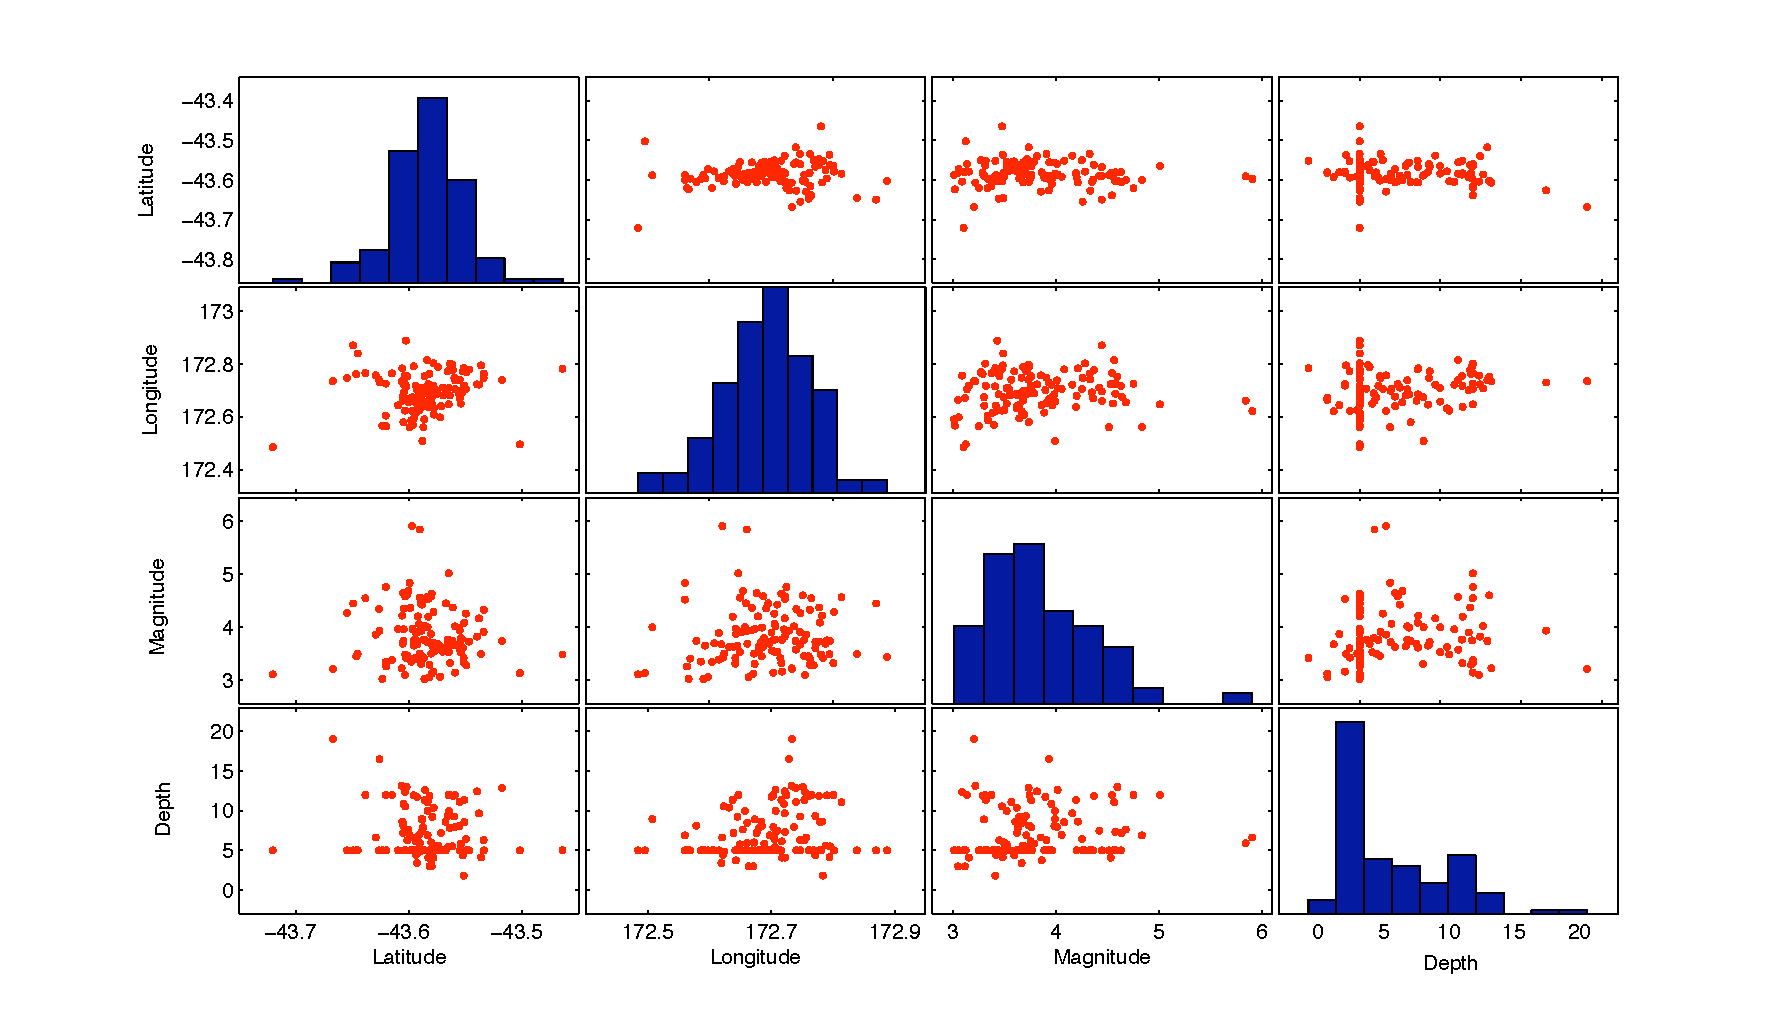
\includegraphics[width=6.5in]{figures/NZEQ20110222ChchLtLnMgDpScatterMatrixPlot}}
\end{figure}


\begin{labwork}\label{LW:NZEQChCch20110222EDA}
Try to understand how to manipulate time stamps of events in \Matlab and the Figures being output by following the comments in the script file {\tt NZEQChCch20110222EDA.m}.
\begin{VrbM}
>> NZEQChCch20110222
ans =   145    14
ans =   145    14
ans =   124    14
ans =   145    14
ans =   145    14
ans =   124    14
ans = 22-Feb-2011 00:00:31
ans = 22-Feb-2011 23:50:01
\end{VrbM}
\VrbMf[label=NZEQChCch20110222EDA.m]{scripts/NZEQChCch20110222EDA.m}
\end{labwork}

\subsubsection{Geostatistical exploratory data analysis with Google Earth}

\begin{figure}[htpb]
\caption{Google Earth Visualisation of the earth quakes\label{F:NZEQ20110222ChchLtLnMgDpInGoogleEarthViewFromUSGS}}
\centering   \makebox{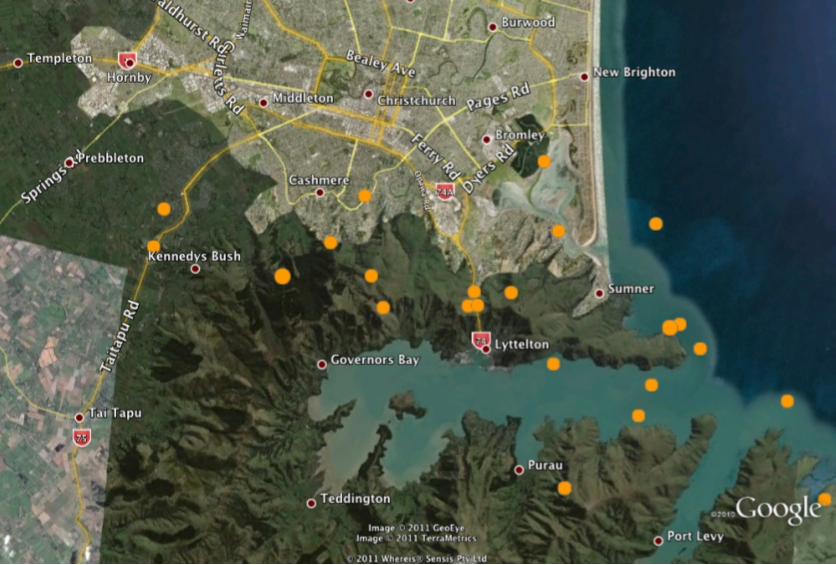
\includegraphics[width=4.5in]{figures/NZEQ20110222ChchLtLnMgDpInGoogleEarthViewFromUSGS}}
\end{figure}

A global search at \href{http://neic.usgs.gov/cgi-bin/epic/epic.cgi}{\url{http://neic.usgs.gov/cgi-bin/epic/epic.cgi}}
%%?SEARCHMETHOD=1&FILEFORMAT=7&SEARCHRANGE=PP&SYEAR=2011&SMONTH=2&SDAY=22&EYEAR=2011&EMONTH=2&EDAY=22&LMAG=&UMAG=&NDEP1=&NDEP2=&IO1=&IO2=&CLAT=0.0&CLON=0.0&CRAD=0.0&SUBMIT=Submit+Search}
with the following parameters:
\begin{verbatim}
Date Range: 2011 2 22 to 2011 2 22 
Catalog: USGS/NEIC (PDE-Q) 
\end{verbatim}
produced 43 earth quakes world-wide, including those in Christchurch as shown in \hyperref[F:NZEQ20110222ChchLtLnMgDpInGoogleEarthViewFromUSGS]{Figure~\ref*{F:NZEQ20110222ChchLtLnMgDpInGoogleEarthViewFromUSGS}}.  One can do a lot more than a mere visualisation with the USGS/NEIC  database of earth-quakes wolrd-wide, the freely available {\tt Google earth} software bundle \href{http://www.google.com/earth/index.html}{\url{http://www.google.com/earth/index.html}} and the freely available \Matlab package {\tt googleearth} from \href{http://www.mathworks.com/matlabcentral/fx_files/12954/4/content/googleearth/html/html_product_page.html}{\url{http://www.mathworks.com/matlabcentral/fx_files/12954/4/content/googleearth/html/html_product_page.html}}.

\subsection{Metereological Data}

New Zealand's meteorological service NIWA provides weather data under it TERMS AND CONDITIONS FOR ACCESS TO DATA (See \url{http://cliflo.niwa.co.nz/doc/terms_print.html}).  We will explore some data of rainfall and temperatures from NIWA.

\subsubsection{Daily Rainfalls in Christchurch}

%Rainfall Data in Christchurch

Automagic downloading of the data by {\sf Method B} can be done if the data provider allows automated queries.  It can be accomplished by {\tt urlread} for instance.  %Try to download the file



%is being  \work.  But you can t

Paul Brouwers has a basic CliFlo datafeed on \url{http://www.math.canterbury.ac.nz/php/lib/cliflo/rainfall.php}.  %?range=20100425:20100501
This returns the date and rainfall in milli meters as measured from the CHCH aeroclub station. It is assumed that days without readings would not be listed. %It expects a range parameter such as: ?range=20100425:20100501 The first number is the starting search date (YYYYMMDD). Colon as separator. The first number is the ending search date (YYYYMMDD). CliFlo limits us to 2 million rows for the subscription and 40,000 rows per query (which is equivalent of over 100 years of data, so I we're safe - 
The data doesn't go back much before 1944.

%wetdataURL = 'http://www.math.canterbury.ac.nz/php/lib/cliflo/?range=20100101:20100510' wetdataURL = 'http://www.math.canterbury.ac.nz/php/lib/cliflo/rainfall.php'
%\work 


\begin{labwork}\label{LW:ChchDailyRainfallSince}
Understand how \hyperref[F:ChchDailyRainfallSince]{Figure~\ref*{F:ChchDailyRainfallSince}} is obtained by the script file {\tt RainFallsInChch.m} by typing and following the comments:

\begin{VrbM}
>> RainFallsInChch
RainFallsChch =     [24312x1 int32]    [24312x1 double]
ans =       24312           2
FirstDayOfData =    19430802
LastDayOfData =    20100721
\end{VrbM}

\VrbMf[label=RainFallsInChch.m]{scripts/RainFallsInChch.m}
\end{labwork}

\begin{figure}[htpb]
\caption{Daily rainfalls in Christchurch since March 27 2010 \label{F:ChchDailyRainfallSince}}
\centering   \makebox{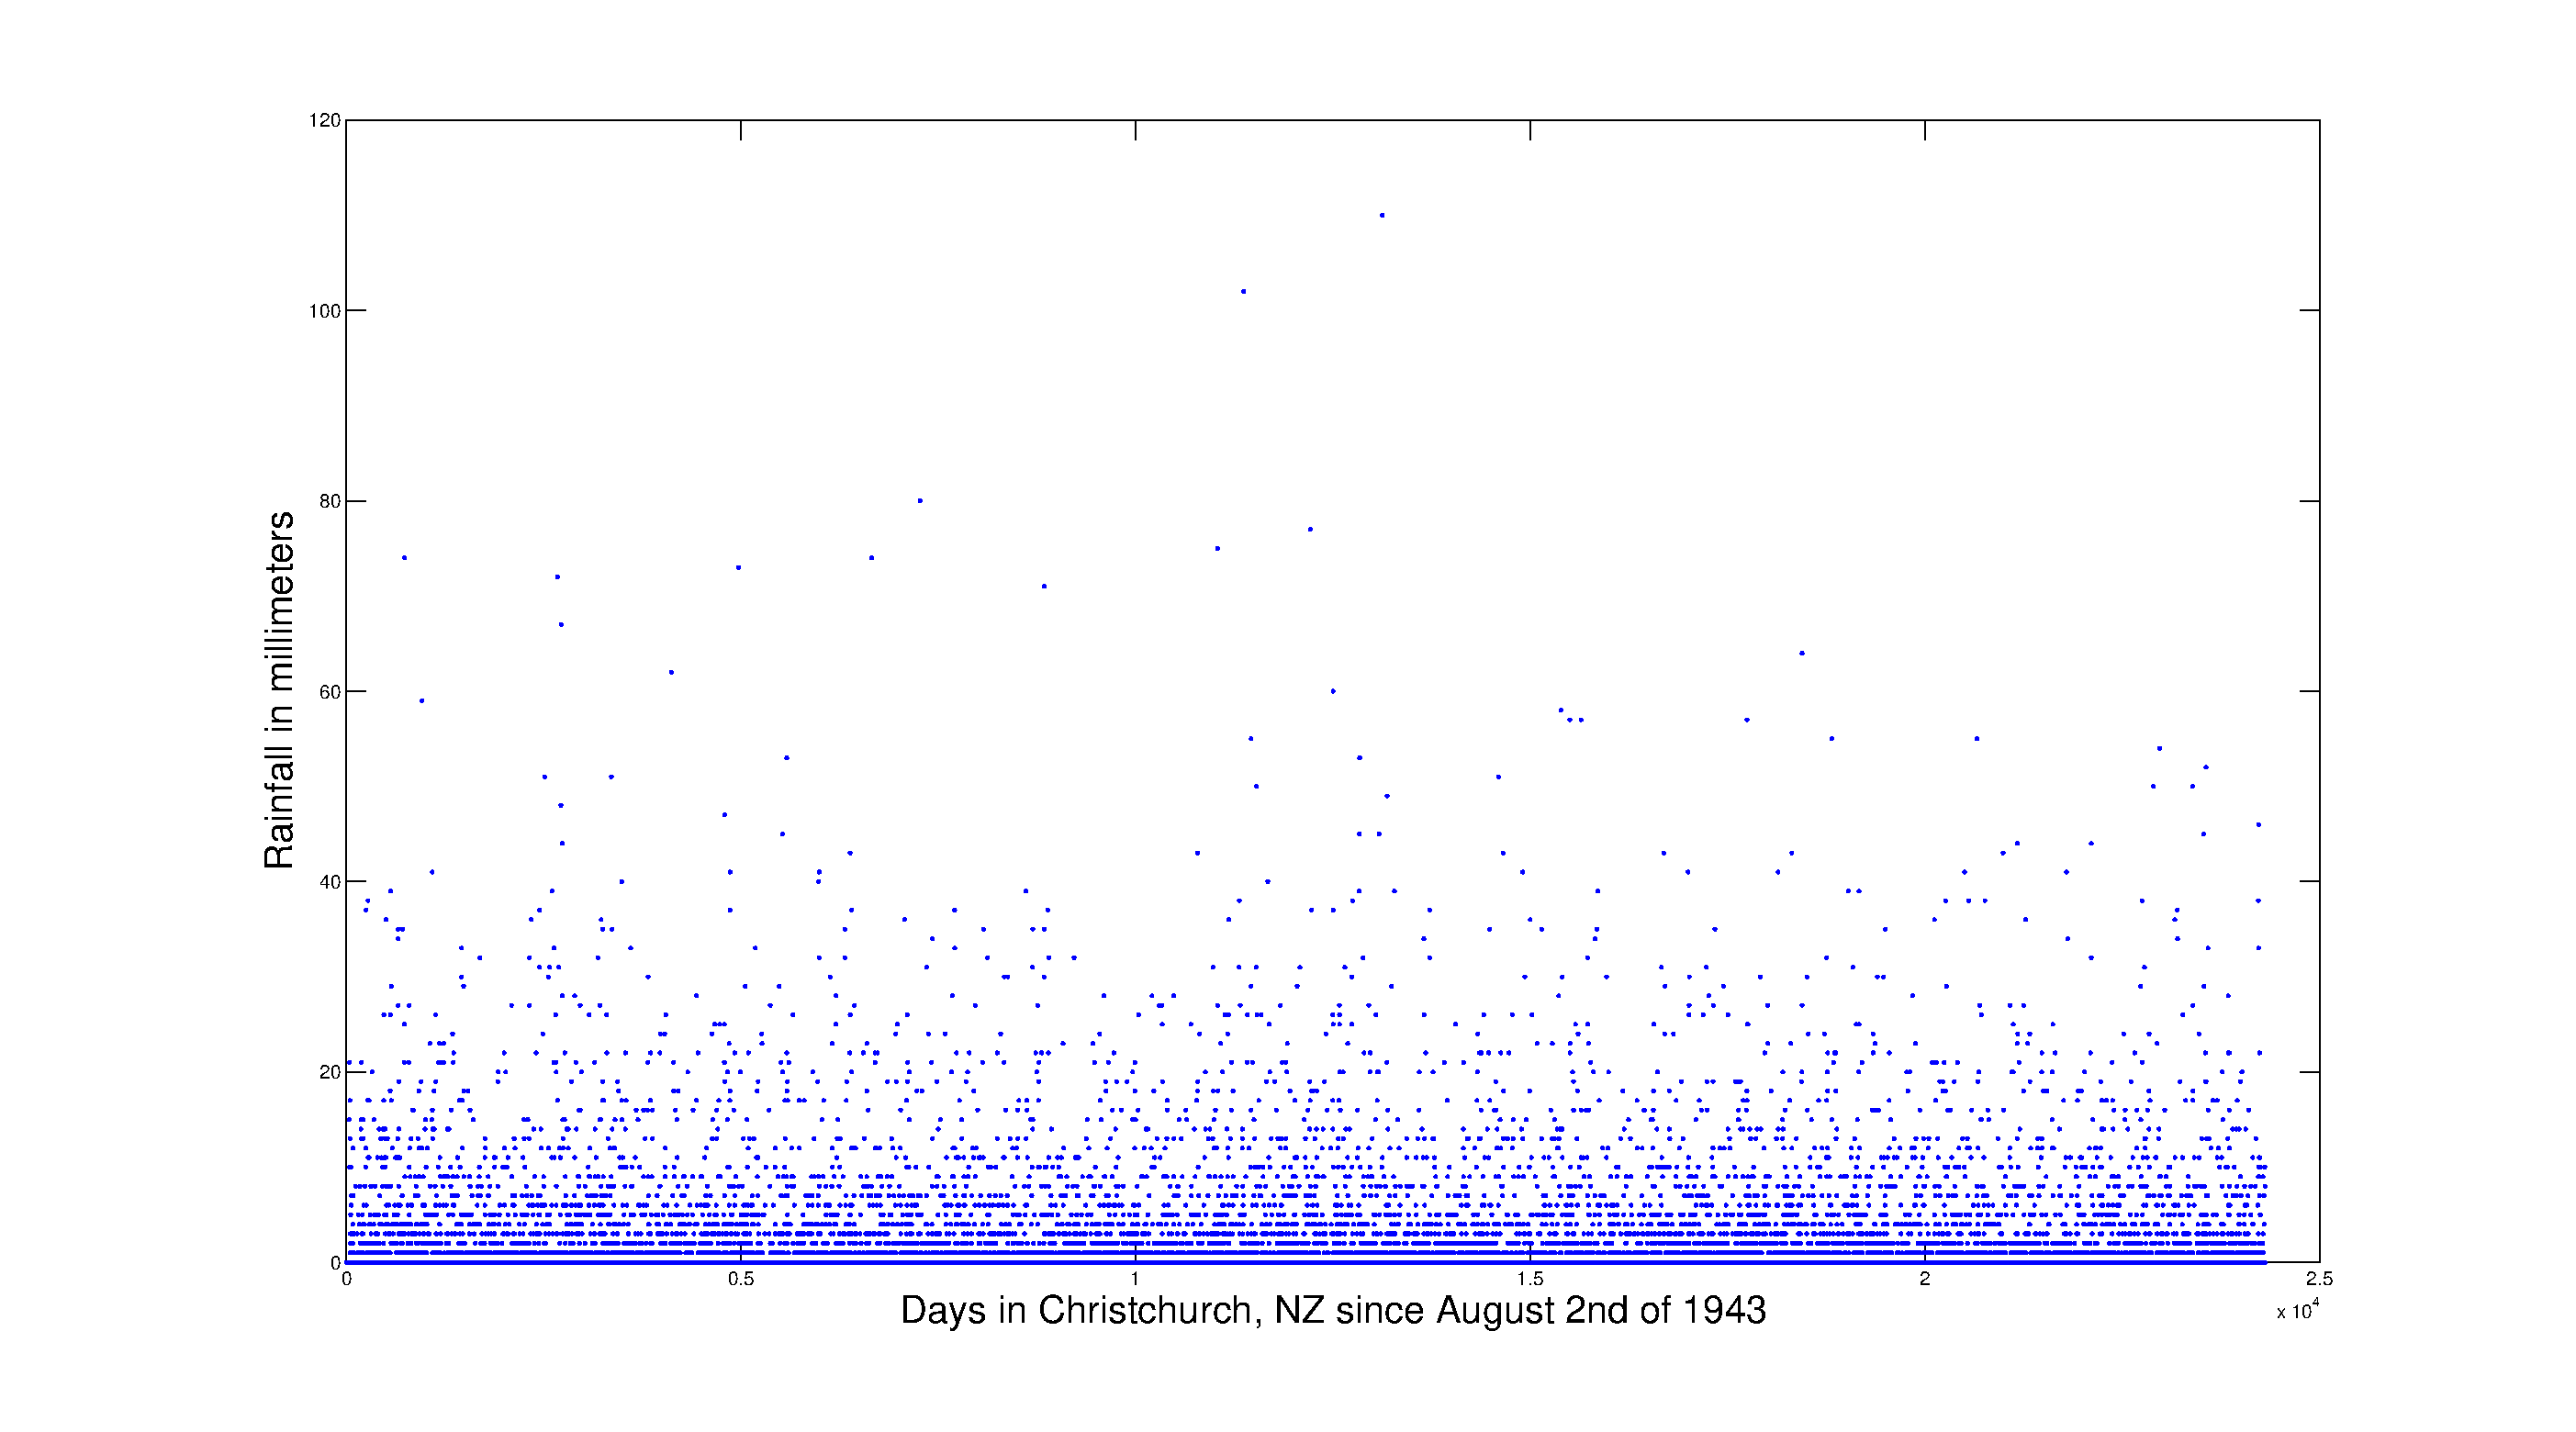
\includegraphics[width=6.5in]{figures/ChchDailyRainfallSince}}
\end{figure}

\subsubsection{Daily Temperatures in Christchurch}


\begin{labwork}\label{LW:ChchTempsLoad}
Understand how \hyperref[F:ChchTemps365DaysSince20100327]{Figure~\ref*{F:ChchTemps365DaysSince20100327}} is being generated by following the comments in the script file {\tt ChchTempsLoad.m} by typing:
\begin{VrbM}
>> ChchTempsLoad
\end{VrbM}
\VrbMf[label=ChchTempsLoad.m]{scripts/ChchTempsLoad.m}
\end{labwork}

\begin{figure}[htpb]
\caption{Daily temperatures in Christchurch for one year since March 27 2010 \label{F:ChchTemps365DaysSince20100327}}
\centering   \makebox{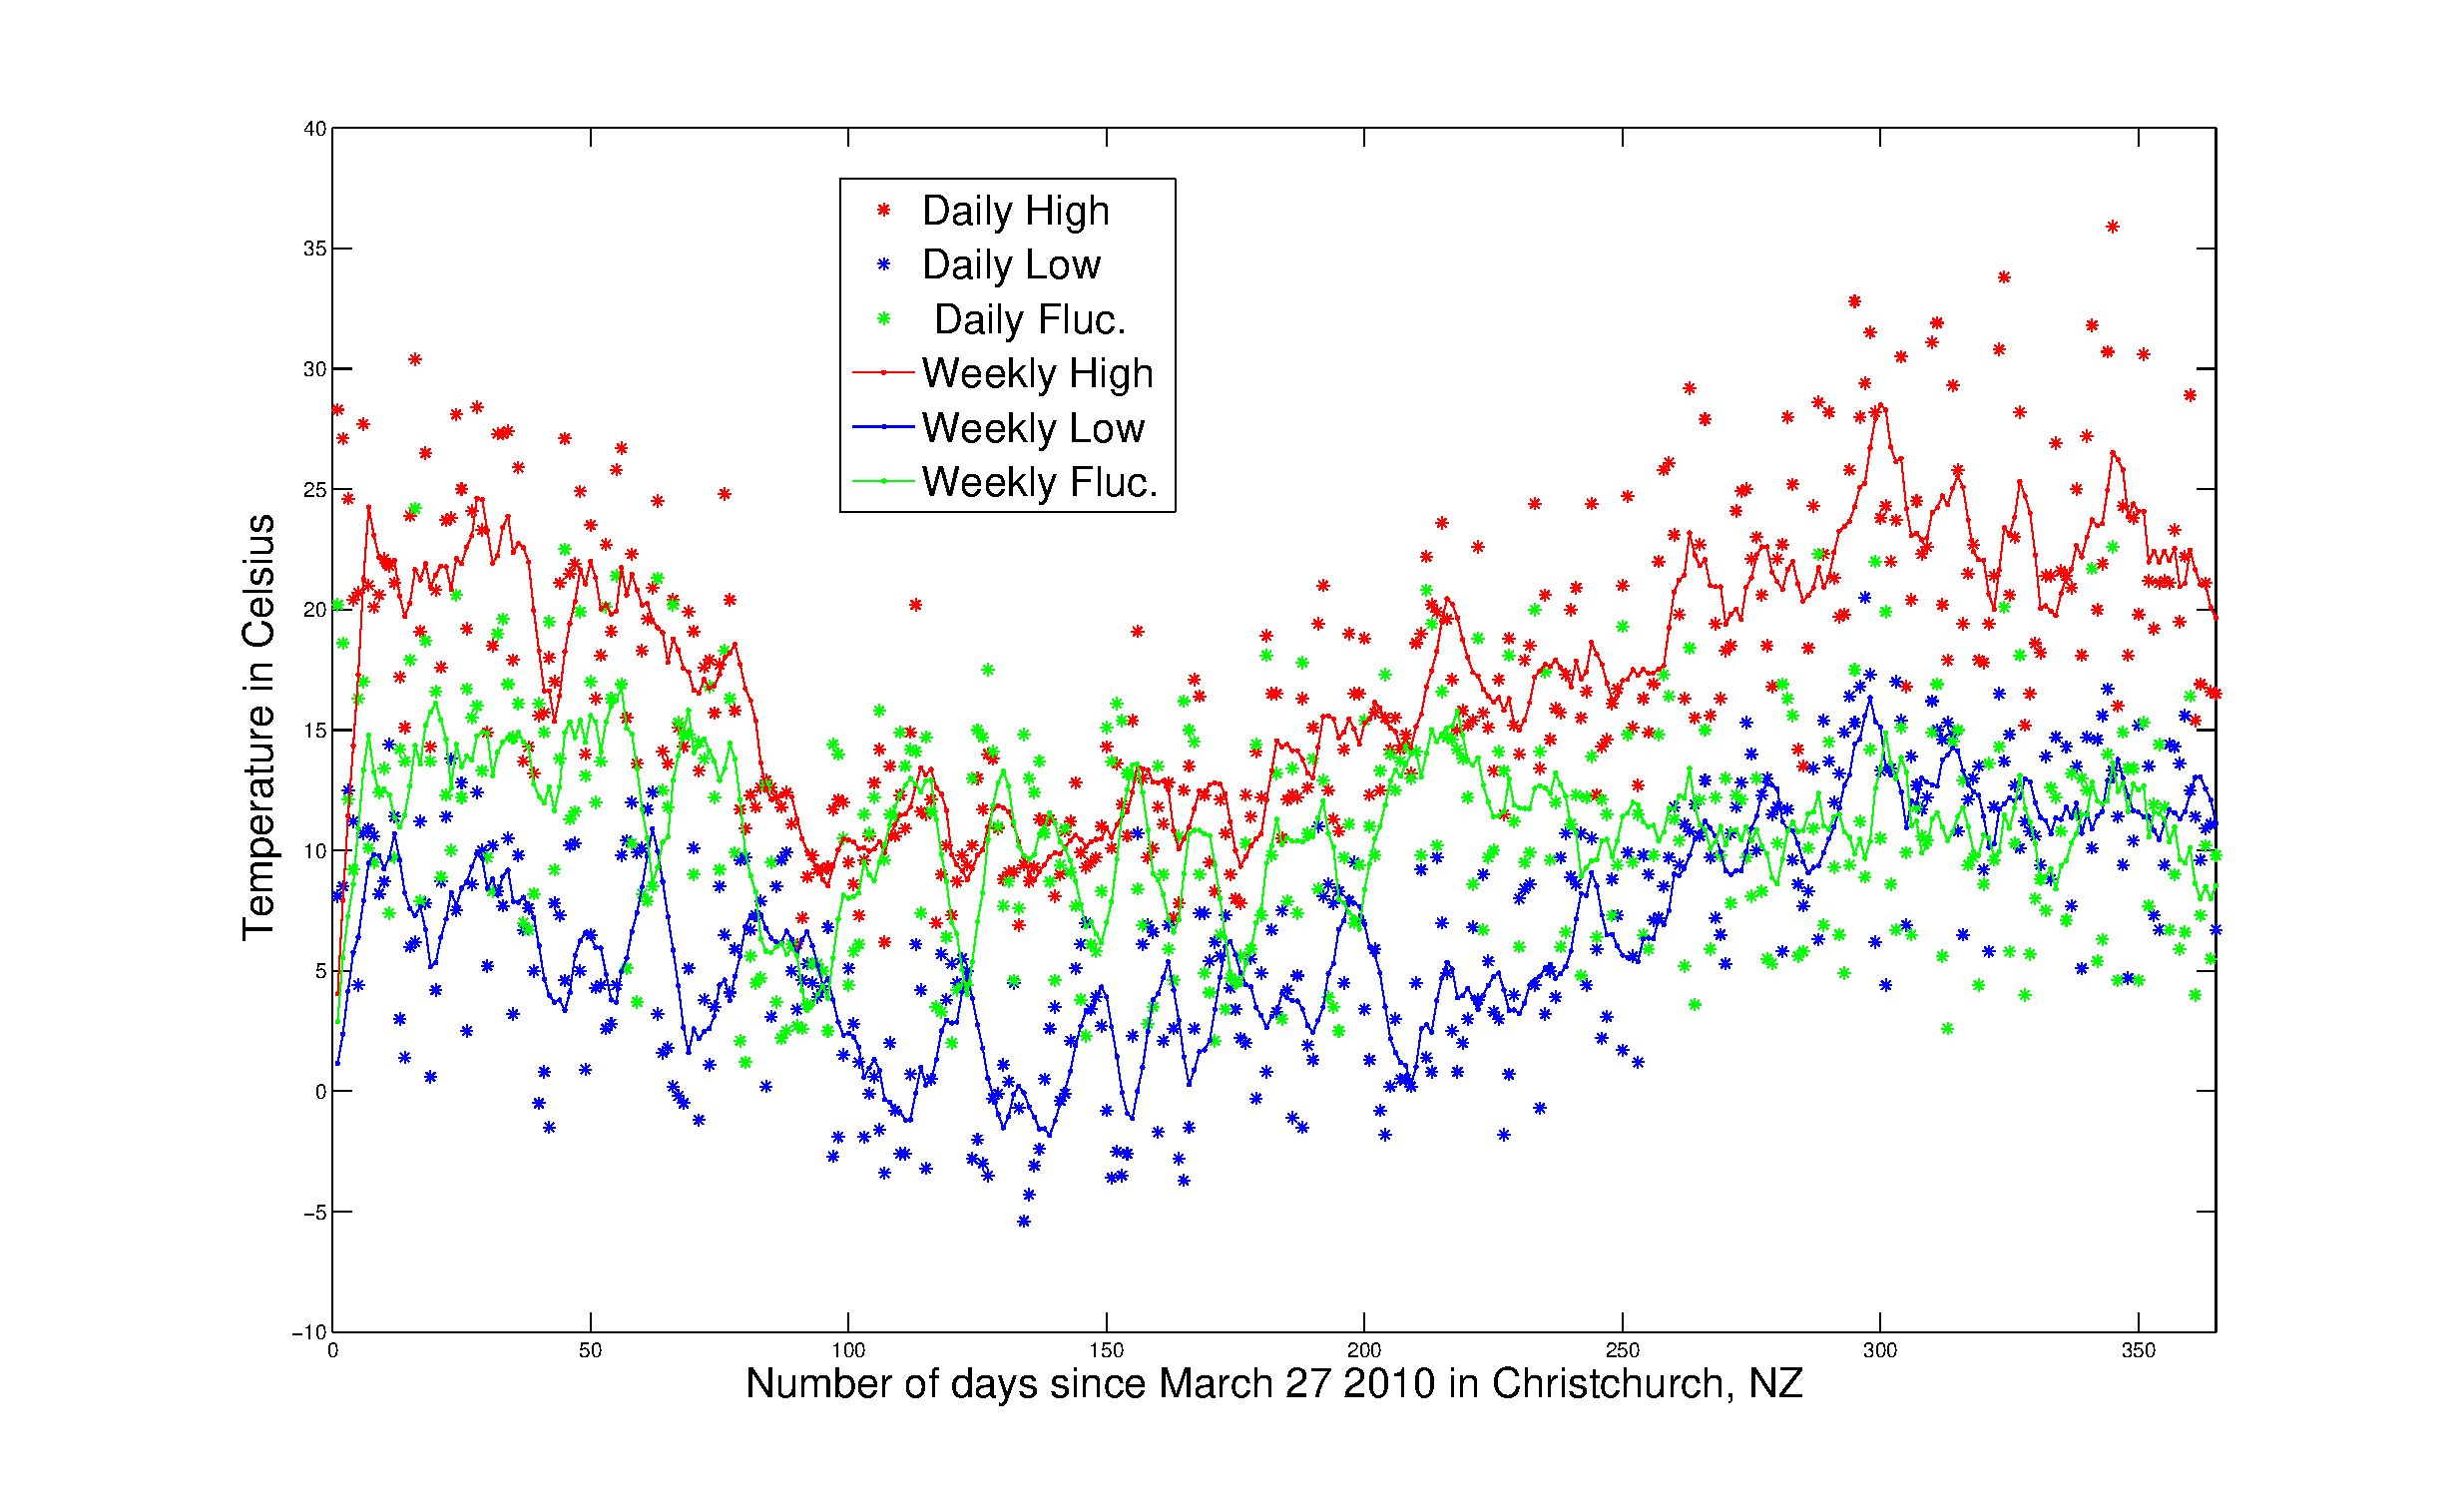
\includegraphics[width=6.5in]{figures/ChchTemps365DaysSince20100327}}
\end{figure}

\subsection{Textual Data}

Processing and analysing textual data to make a decision is another important computational statistical experiment. An obvious example  is machine translation and a less obvious one is exploratory data analysis of the textual content of 
\begin{itemize}
\item a large document
\item twitter messages within an online social network of interest
\item etc.
\end{itemize}

An interesting document with a current affairs projection is the Joint Operating Environment 2010 Report by the US Department of Defense.  This document was downloaded from \href{http://www.jfcom.mil/newslink/storyarchive/2010/JOE_2010_o.pdf}{\url{http://www.jfcom.mil/newslink/storyarchive/2010/JOE_2010_o.pdf}}.  The first paragraph of this 74 page document (JOE 2010 Reprort) reads:

{\small
ABOUT THIS STUDY The Joint Operating Environment is intended to inform joint concept development and experimentation throughout the Department of Defense. It provides a perspective on future trends, shocks, contexts, and implications for future joint force commanders and other leaders and professionals in the national security field. This document is speculative in nature and does not suppose to predict what will happen in the next twenty-five years. Rather, it is intended to serve as a starting point for discussions about the future security environment at the operational level of war. Inquiries about the Joint Operating Environment should be directed to USJFCOM Public Affairs, 1562 Mitscher Avenue, Suite 200, Norfolk, VA 23551-2488, (757) 836-6555. 

Distribution Statement A: Approved for Public Release
}

\begin{figure}[htpb]
\caption{Wordle of JOE 2010\label{F:joe_vs_wordle}}
\centering   \makebox{
\includegraphics[width=6.5in]{figures/joe_vs_wordle_RaazCroppedPhilWilsonsImage}}
\end{figure}

We can try to produce a statistic of this document by recording the frequency of words in its textual content. Then we can produce a ``word histogram'' or ``word cloud'' to explore the document visually at one of the coarsest possible resolutions of the textual content in the JOE 2010 Report.  The ``word cloud'' shown in \hyperref[F:joe_vs_wordle]{Figure~\ref*{F:joe_vs_wordle}} was produced by Phillip Wilson using {\em wordle} from \href{http://www.wordle.net/}{\url{http://www.wordle.net/}}.  A description from the wordle URL says:

{\small
Wordle is a toy for generating Òword cloudsÓ from text that you provide. The clouds give greater prominence to words that appear more frequently in the source text. You can tweak your clouds with different fonts, layouts, and color schemes. The images you create with Wordle are yours to use however you like. You can print them out, or save them to the Wordle gallery to share with your friends.
}

\begin{labwork}[favourite word cloud]\label{LW:JoeWordle}  This is just for fun.  Produce a ``word cloud'' of your honours thesis or summer project or any other document that fancies your interest by using {\em wordle} from \href{http://www.wordle.net/}{\url{http://www.wordle.net/}}. Play with the aesthetic features to change colour, shapes, etc.\end{labwork}

\subsection{Machine Sensor Data}

Instrumentation of modern machines, such as planes, rockets and cars allow the sensors in the machines to collect live data and dynamically take {\em decisions} and subsequent {\em actions} by executing algorithms to drive their devices in response to the data that is streaming into their sensors.  For example, a rocket may have to adjust its boosters to compensate for the prevailing directional changes in wind in order to keep going up and launch a satellite.  
These types of decisions and actions, theorised by {\em controlled Markov processes}, typically arise in various fields of engineering such as, aerospace, civil, electrical, mechanical, robotics, etc.

In an observational setting, without an associated control problem, one can use machine sensor data to get information about some state of the system or phenomenon, i.e., what is it doing? or where is it?, etc.  Sometimes sensors are attached to a sample of individuals from a  wild population, say Emperor Penguins in Antarctica where the phenomenon of interest may be the diving habits of this species after the eggs hatch.  As an other example we can attach sensors to a double pendulum and find what it is doing when we give it a spin.

Based on such observational data the experimenter typically tries to learn about the behaviour of the system from the sensor data to estimate parameters, test hypotheses, etc. Such types of experiments are typically performed by scientists in various fields of science, such as, astronomy, biology, chemistry, geology, physics, etc.  

\subsubsection{Chaotic Time Series of a Double Pendulum}

\begin{figure}[htbp]
\begin{center}
{\scriptsize
\begin{tabular}{ccc}
A: DP Schematic & B: Streaming DP data & C: Enclosures of two initially close trajectories\\
  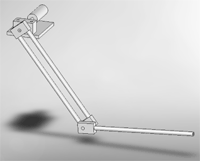
\includegraphics[scale=0.5]{figures/dp} &
  \includegraphics[scale=0.66]{figures/vlcsnap-2010-01-13-10h11m08s38_closeup} &
  \includegraphics[height=3cm,width=6.75cm]{figures/divergence_piers}
\end{tabular}
}
\end{center}
\caption{Double Pendulum}
\label{F:DP3}
\end{figure}

Sensors called {\em optical encoders} have been attached to the top end of each arm of a chaotic double pendulum in order to obtain the angular position of each arm through time as shown in \hyperref[F:DP3]{Figure~\ref*{F:DP3}}.  Time series of the angular position of each arm for two trajectories that were initialized very similarly, say the angles of each arm of the double pendulum are almost the same at the initial time of release.  Note how quickly the two trajectories diverge!  System with such a sensitivity to initial conditions are said to be {\em chaotic}.

\begin{labwork}[A Challenging Task]\label{LW:DPtrajectoryparsing}  Try this if you are interested.  Read any of the needed details about the design and fabrication of  the double pendulum at \href{http://www.math.canterbury.ac.nz/~r.sainudiin/lmse/double-pendulum/}{\url{http://www.math.canterbury.ac.nz/~r.sainudiin/lmse/double-pendulum/}}.  Then use \Matlab to generate a plot similar to \hyperref[F:DP3]{Figure~\ref*{F:DP3}(C)} using time series data of {\sf trajectory~1} and {\sf  trajectory~2} linked from the bottom of the above URL.
 \end{labwork}

\comment{
\subsection{Biological Data}
\work
}

\section{Exercises in Statistics}\label{S:xsStatistics}
\begin{ExerciseList}
\Exercise What is the sample mean and sample variance of the following dataset:
\[
1, 3, 2, 1, 2, 3, 3
\]
\Answer Apply the formulas for the sample mean, $\overline{X_7}$, and sample variance.
\end{ExerciseList}



%\remove
%%%%%%%%%%%%%%%%%%%%%%%%%%%%%%%%%%%%%%%%%%%%%%%%%%%%%%%%%%%%%%%%%%%%%%%%%%%%%%
%%%% snipped above into csebook


%\newpage

%\section{Exercises}\label{Exs:onRV}

%\begin{ExerciseList}

%\end{ExerciseList}
%\newpage
